%%%%%%%%%%%%%%%%%%%%%%%%%%%%%%%%%%%%%%%%%%%%%%%%%%%%%%%%%%%%%%%
%% OXFORD THESIS TEMPLATE

% Use this template to produce a standard thesis that meets the Oxford University requirements for DPhil submission
%
% Originally by Keith A. Gillow (gillow@maths.ox.ac.uk), 1997
% Modified by Sam Evans (sam@samuelevansresearch.org), 2007
% Modified by John McManigle (john@oxfordechoes.com), 2015
% Modified by Ulrik Lyngs (ulrik.lyngs@cs.ox.ac.uk), 2018, for use with R Markdown
%
% Ulrik Lyngs, 25 Nov 2018: Following John McManigle, broad permissions are granted to use, modify, and distribute this software
% as specified in the MIT License included in this distribution's LICENSE file.
%
% John tried to comment this file extensively, so read through it to see how to use the various options.  Remember
% that in LaTeX, any line starting with a % is NOT executed.  Several places below, you have a choice of which line to use
% out of multiple options (eg draft vs final, for PDF vs for binding, etc.)  When you pick one, add a % to the beginning of
% the lines you don't want.


%%%%% CHOOSE PAGE LAYOUT
% The most common choices should be below.  You can also do other things, like replacing "a4paper" with "letterpaper", etc.

% This one will format for two-sided binding (ie left and right pages have mirror margins; blank pages inserted where needed):
%\documentclass[a4paper,twoside]{templates/ociamthesis}
% This one will format for one-sided binding (ie left margin > right margin; no extra blank pages):
%\documentclass[a4paper]{ociamthesis}
% This one will format for PDF output (ie equal margins, no extra blank pages):
%\documentclass[a4paper,nobind]{templates/ociamthesis}
%UL 2 Dec 2018: pass this in from YAML
\documentclass[a4paper, nobind]{templates/ociamthesis}

% UL 5 January 2021 - add packages used by kableExtra
\usepackage{booktabs}
\usepackage{longtable}
\usepackage{array}
\usepackage{multirow}
\usepackage{wrapfig}
\usepackage{colortbl}
\usepackage{pdflscape}
\usepackage{tabu}
\usepackage{threeparttable}
\usepackage{threeparttablex}
\usepackage[normalem]{ulem}
\usepackage{makecell}
\usepackage[colorlinks=false,pdfpagelabels,hidelinks=true]{hyperref}
\usepackage{float}

%UL set section header spacing
\usepackage{titlesec}
% 
\titlespacing\subsubsection{0pt}{24pt plus 4pt minus 2pt}{0pt plus 2pt minus 2pt}

% UL 30 Nov 2018 pandoc puts lists in 'tightlist' command when no space between bullet points in Rmd file
\providecommand{\tightlist}{%
  \setlength{\itemsep}{0pt}\setlength{\parskip}{0pt}}
 
% UL 1 Dec 2018, fix to include code in shaded environments

%UL set whitespace around verbatim environments
\usepackage{etoolbox}
\makeatletter
\preto{\@verbatim}{\topsep=0pt \partopsep=0pt }
\makeatother

%UL 26 Mar 2019, enable strikethrough
\usepackage[normalem]{ulem}

%UL use soul package for correction highlighting
\usepackage{color, soul}
\usepackage{xcolor}
\definecolor{correctioncolor}{HTML}{CCCCFF}
\sethlcolor{correctioncolor}
\newcommand{\ctext}[3][RGB]{%
  \begingroup
  \definecolor{hlcolor}{#1}{#2}\sethlcolor{hlcolor}%
  \hl{#3}%
  \endgroup
}
\soulregister\ref7
\soulregister\cite7
\soulregister\autocite7
\soulregister\textcite7
\soulregister\pageref7

%%%%%%% PAGE HEADERS AND FOOTERS %%%%%%%%%
\usepackage{fancyhdr}
\setlength{\headheight}{15pt}
\fancyhf{} % clear the header and footers
\pagestyle{fancy}
\renewcommand{\chaptermark}[1]{\markboth{\thechapter. #1}{\thechapter. #1}}
\renewcommand{\sectionmark}[1]{\markright{\thesection. #1}} 
\renewcommand{\headrulewidth}{0pt}

\fancyhead[LO]{\emph{\leftmark}} 
\fancyhead[RE]{\emph{\rightmark}} 

% UL page number position 
\fancyfoot[C]{\emph{\thepage}} %regular pages
\fancypagestyle{plain}{\fancyhf{}\fancyfoot[C]{\emph{\thepage}}} %chapter pages

% JEM fix header on cleared pages for openright
\def\cleardoublepage{\clearpage\if@twoside \ifodd\c@page\else
   \hbox{}
   \fancyfoot[C]{}
   \newpage
   \if@twocolumn\hbox{}\newpage
   \fi
   \fancyhead[LO]{\emph{\leftmark}} 
   \fancyhead[RE]{\emph{\rightmark}} 
   \fi\fi}


%%%%% SELECT YOUR DRAFT OPTIONS
% This adds a "DRAFT" footer to every normal page.  (The first page of each chapter is not a "normal" page.)

% This highlights (in blue) corrections marked with (for words) \mccorrect{blah} or (for whole
% paragraphs) \begin{mccorrection} . . . \end{mccorrection}.  This can be useful for sending a PDF of
% your corrected thesis to your examiners for review.  Turn it off, and the blue disappears.
\correctionstrue

%%%%% BIBLIOGRAPHY SETUP
% Note that your bibliography will require some tweaking depending on your department, preferred format, etc.
% If you've not used LaTeX before, I recommend reading a little about biblatex/biber and getting started with it.
% If you're already a LaTeX pro and are used to natbib or something, modify as necessary.
% Either way, you'll have to choose and configure an appropriate bibliography format...


\usepackage[style=authoryear, sorting=nyt, backend=biber, maxcitenames=2, useprefix, doi=true, isbn=false, uniquename=false]{biblatex}
\newcommand*{\bibtitle}{Works Cited}

\addbibresource{references.bib}


% This makes the bibliography left-aligned (not 'justified') and slightly smaller font.
\renewcommand*{\bibfont}{\raggedright\small}


% Uncomment this if you want equation numbers per section (2.3.12), instead of per chapter (2.18):
%\numberwithin{equation}{subsection}


%%%%% THESIS / TITLE PAGE INFORMATION
% Everybody needs to complete the following:
\title{Bayesian spatio-temporal methods for small-area estimation of HIV indicators}
\author{Adam Howes}
\college{Department of Mathematics}

% Master's candidates who require the alternate title page (with candidate number and word count)
% must also un-comment and complete the following three lines:

% Uncomment the following line if your degree also includes exams (eg most masters):
%\renewcommand{\submittedtext}{Submitted in partial completion of the}
% Your full degree name.  (But remember that DPhils aren't "in" anything.  They're just DPhils.)
\degree{Doctor of Philosophy}
% Term and year of submission, or date if your board requires (eg most masters)
\degreedate{December 2023}


%%%%% YOUR OWN PERSONAL MACROS
% This is a good place to dump your own LaTeX macros as they come up.

\usepackage{pifont}
\usepackage{amsmath}
\usepackage{tabularx}
\usepackage{bm}

\newcommand{\Sc}{\mathcal{S}}
\newcommand{\R}{\mathcal{R}}
\newcommand{\bR}{\mathbf{R}}
\newcommand{\N}{\mathcal{N}}
\newcommand{\X}{\mathcal{X}} 
\newcommand{\m}{\mathbf{m}}
\newcommand{\bu}{\mathbf{u}}
\newcommand{\bv}{\mathbf{v}}
\newcommand{\w}{\mathbf{w}}
\newcommand{\x}{\mathbf{x}}
\newcommand{\y}{\boldsymbol{\mathbf{y}}}
\newcommand{\z}{\mathbf{z}}
\newcommand{\bb}{\mathbf{b}}
\newcommand{\Hb}{\mathbf{H}}
\newcommand{\bphi}{\boldsymbol{\mathbf{\phi}}}
\newcommand{\brho}{\bm{\rho}}
\newcommand{\btheta}{\bm{\theta}}
\newcommand{\bmeta}{\bm{\eta}}
\newcommand{\bvartheta}{\bm{\vartheta}}
\newcommand{\bmu}{\bm{\mu}}

\newcommand{\cmark}{\ding{51}}
\newcommand{\xmark}{\ding{55}}

\DeclareMathOperator*{\argmin}{arg\,min}
\DeclareMathOperator*{\argmax}{arg\,max}

% To make text superscripts shortcuts
	\renewcommand{\th}{\textsuperscript{th}} % ex: I won 4\th place
	\newcommand{\nd}{\textsuperscript{nd}}
	\renewcommand{\st}{\textsuperscript{st}}
	\newcommand{\rd}{\textsuperscript{rd}}

%%%%% THE ACTUAL DOCUMENT STARTS HERE
\begin{document}

%%%%% CHOOSE YOUR LINE SPACING HERE
% This is the official option.  Use it for your submission copy and library copy:
\setlength{\textbaselineskip}{22pt plus2pt}
% This is closer spacing (about 1.5-spaced) that you might prefer for your personal copies:
%\setlength{\textbaselineskip}{18pt plus2pt minus1pt}

% You can set the spacing here for the roman-numbered pages (acknowledgements, table of contents, etc.)
\setlength{\frontmatterbaselineskip}{17pt plus1pt minus1pt}

% UL: You can set the line and paragraph spacing here for the separate abstract page to be handed in to Examination schools
\setlength{\abstractseparatelineskip}{13pt plus1pt minus1pt}
\setlength{\abstractseparateparskip}{0pt plus 1pt}

% UL: You can set the general paragraph spacing here - I've set it to 2pt (was 0) so
% it's less claustrophobic
\setlength{\parskip}{2pt plus 1pt}

%
% Oxford University logo on title page
%
\def\crest{{
\includegraphics{templates/ic-small.pdf}}}
\renewcommand{\university}{Imperial College London}
\renewcommand{\submittedtext}{In partial fulfillment of the requirements for the degree of}


% Leave this line alone; it gets things started for the real document.
\setlength{\baselineskip}{\textbaselineskip}


%%%%% CHOOSE YOUR SECTION NUMBERING DEPTH HERE
% You have two choices.  First, how far down are sections numbered?  (Below that, they're named but
% don't get numbers.)  Second, what level of section appears in the table of contents?  These don't have
% to match: you can have numbered sections that don't show up in the ToC, or unnumbered sections that
% do.  Throughout, 0 = chapter; 1 = section; 2 = subsection; 3 = subsubsection, 4 = paragraph...

% The level that gets a number:
\setcounter{secnumdepth}{2}
% The level that shows up in the ToC:
\setcounter{tocdepth}{1}


%%%%% ABSTRACT SEPARATE
% This is used to create the separate, one-page abstract that you are required to hand into the Exam
% Schools.  You can comment it out to generate a PDF for printing or whatnot.

% JEM: Pages are roman numbered from here, though page numbers are invisible until ToC.  This is in
% keeping with most typesetting conventions.
\begin{romanpages}

% Title page is created here
\maketitle

%%%%% COPYRIGHT -- added by ATH.
\begin{copyrights}
  The copyright of this thesis rests with the author. Unless otherwise indicated, its contents are licensed under a Creative Commons Attribution-Non Commercial 4.0 International Licence (CC BY-NC).
  Under this licence, you may copy and redistribute the material in any medium or format. You may also create and distribute modified versions of the work.
  This is on the condition that: you credit the author and do not use it, or any derivative works, for a commercial purpose.
  When reusing or sharing this work, ensure you make the licence terms clear to others by naming the licence and linking to the licence text.
  Where a work has been adapted, you should indicate that the work has been changed and describe those changes.
  Please seek permission from the copyright holder for uses of this work that are not included in this licence or permitted under UK Copyright Law.
\end{copyrights}

%%%%% ORIGINALITY -- added by ATH.
\begin{originality}
  This thesis, and the work presented in it, is work that I conducted myself.
  In all cases where I describe others' work, I provide appropriate references.
\end{originality}

%%%%% DEDICATION -- If you'd like one, un-comment the following.
\begin{dedication}
  \textit{For someone, or something.}
\end{dedication}

%%%%% ACKNOWLEDGEMENTS -- Nothing to do here except comment out if you don't want it.
\begin{acknowledgements}
 	Thanks to my supervisors Seth Flaxman and Jeff Eaton for their guidance and mentorship.
 I am grateful for the research environment provided by the Modern Statistics and Statistical Machine Learning Centre for Doctoral Training at Imperial and Oxford, the HIV Inference Group at Imperial, and the Machine Learning and Global Health Network across the UK, Denmark, Germany and Singapore.
 Thanks to Mike McLaren, Kevin Esvelt, the Nucleic Acid Observatory team, and the Sculpting Evolution lab for hosting my visit to the MIT Media Lab.
 Thanks to Alex Stringer, and the Department of Statistics and Actuarial Science for hosting my visit to the University of Waterloo.
 My sense for what matters has been shaped (arguably improved) by the Effective Altruism community.
 This research was made possible by funding provided by the Bill \& Melinda Gates Foundation and EPSRC.

 \begin{flushright}
 Adam Howes \\
 Imperial College London\\
 December 2023
 \end{flushright}
\end{acknowledgements}

%%%%% ABSTRACT -- Nothing to do here except comment out if you don't want it.
\begin{abstract}
	Progress towards ending AIDS as a public health threat by 2030 is not being made fast enough.
Effective public health response requires accurate, timely, high-resolution estimates of epidemic and demographic indicators.
Limitations of available data make obtaining these estimates difficult.
I developed and applied Bayesian spatio-temporal methods to meet this challenge.
First, I examined models for area-level spatial structure.
Second, I estimated district-level HIV risk group proportions, enabling behavioural prioritisation of prevention services, as put forward in the Global AIDS Strategy.
Finally, I developed a novel deterministic Bayesian inference method, combining adaptive Gauss-Hermite quadrature with principal component analysis, motivated by the Naomi district-level model of HIV indicators.
Together, the contributions in this thesis help to guide precision HIV policy in sub-Saharan Africa, as well as advancing Bayesian methods for spatio-temporal data.
\end{abstract}

%%%%% MINI TABLES
% This lays the groundwork for per-chapter, mini tables of contents.  Comment the following line
% (and remove \minitoc from the chapter files) if you don't want this.  Un-comment either of the
% next two lines if you want a per-chapter list of figures or tables.
  \dominitoc % include a mini table of contents

% This aligns the bottom of the text of each page.  It generally makes things look better.
\flushbottom

% This is where the whole-document ToC appears:
\tableofcontents

\listoffigures
	\mtcaddchapter
  	% \mtcaddchapter is needed when adding a non-chapter (but chapter-like) entity to avoid confusing minitoc

% Uncomment to generate a list of tables:
\listoftables
  \mtcaddchapter
%%%%% LIST OF ABBREVIATIONS
% This example includes a list of abbreviations.  Look at text/abbreviations.tex to see how that file is
% formatted.  The template can handle any kind of list though, so this might be a good place for a
% glossary, etc.
%tibble(
%  Term = c("HIV"),
%  Abbreviation = C("Human Immunodeficiency Virus")
%  ) %>%
%  arrange(Term) %>%
%  kable(booktab = TRUE, escape = FALSE, "latex")

% After writing, reorder these as they appear in the text

% First parameter can be changed eg to "Glossary" or something.
% Second parameter is the max length of bold terms.
\begin{mclistof}{List of Abbreviations}{3.2cm}

\item[HIV] Human Immunodeficiency Virus.
\item[DALY] Disability Adjusted Life Year.
\item[AIDS] Acquired ImmunoDeficiency Syndrome.
\item[UNAIDS] The Joint United Nations Programme on HIV/AIDS.
\item[PEPFAR] President’s Emergency Plan for AIDS Relief.
\item[Global Fund] Global Fund to Fight AIDS, Tuberculosis, and Malaria.
\item[HIV] Demographic and Health Surveys.
\item[AIS] AIDS Indicator Survey.
\item[PrEP] Pre-Exposure Prophylaxis.
\item[PEP] Post-Exposure Prophylaxis.
\item[FSW] Female Sex Worker(s).
\item[MSM] Men who have Sex with Men.
\item[PWID] People Who Inject Drugs.
\item[TGP] Transgender People
\item[ANC] Antenatal Clinic.
\item[CDC] Centers for Disease Control and Prevention.
\item[UAT] Unlinked Anonymous Testing.
\item[PMTCT] Prevention of Mother-to-Child Transmission.
\item[PLHIV] People Living with HIV.
\item[TaSP] Treatment as Prevention.
\item[STI] Sexually Transmitted Infection.
\item[ART] Antiretroviral Therapy.
\item[VMMC] Voluntary Medical Male Circumcision.
\item[DHS] Demographic and Health Surveys.
\item[PHIA] Population-based HIV Impact Assessment.
\item[SSA] Sub-Saharan Africa.

\item[DDC] Data Defect Correlation.
\item[MCMC] Markov Chain Monte Carlo.
\item[NUTS] No-U-Turn Sampler.
\item[VI] Variational Inference.
\item[INLA] Integrated Nested Laplace Approximation.
\item[GP] Gaussian Process.
\item[CAR] Conditionally Auto-regressive.
\item[ICAR] Intrinsic Conditionally Auto-regressive.
\item[SAE] Small-Area Estimation.
\item[GMRF] Gaussian Markov Random Field.
\item[HMC] Hamiltonian Monte Carlo.
\item[GMRF] Gauss-Markov Random Field.
\item[HMC] Hamiltonian Monte Carlo.
\item[LM] Linear Model.
\item[GLM] Generalised Linear Model.
\item[GLMM] Generalised Linear Mixed effects Model.
\item[LGM] Latent Gaussian Model.
\item[ELGM] Extended Latent Gaussian Model.
\item[BF] Bayes Factor.
\item[CPO] Conditional Predictive Ordinate.
\item[DIC] Deviance Information Criterion.
\item[BIC] Bayesian Information Criterion.
\item[WAIC] Watanabe-Akaike Information Criterion.
\item[SR] Scoring Rule.
\item[SPSR] Strictly Proper Scoring Rule.
\item[CRPS] Continuous Ranked Probability Score.
\item[LS] Log Score.
\item[PIT] Probability Integral Transform.
\item[ECDF] Empirical Cumulative Difference Function.
\item[ESS] Effective Sample Size.
\item[IID] Independent and Identically Distributed.
\item[PPL] Probabilistic Programming Language.
\item[CCD] Central Composite Design.
\item[EB] Empirical Bayes.
\item[AGHQ] Adaptive Gauss-Hermite Quadrature.

\end{mclistof} 


%%%%% LIST OF NOTATION
\begin{mclistof}{List of Notations}{3.2cm}

\item[$\rho$] HIV prevalence.
\item[$\lambda$] HIV incidence.
\item[$\alpha$] ART coverage.
\item[$\mathcal{S}$] Spatial study region $\mathcal{S} \subseteq \mathbb{R}^2$.
\item[$s \in \mathcal{S}$] Point location.
\item[$\mathcal{T}$] Temporal study period $\mathcal{T} \subseteq \mathbb{R}$.
\item[$t \in \mathcal{T}$] Time.
\item[$\y$] Data, a $n$-vector.
\item[$\bphi$] Parameters, a $d$-vector $(\phi_1, \ldots, \phi_d)$.
\item[$\x$] Latent field, a $N$-vector $(x_1, \ldots, x_N)$.
\item[$\btheta$] Hyperparameters, a $m$-vector $(\theta_1, \ldots, \theta_m)$.
\item[$x \sim p(x)$] $x$ is distributed according to $p(x)$.
\item[$A_i$] Areal unit.
\item[$A_i \sim A_j$] Adjacency between areal units.
\item[$\mathbf{H}$] Hessian matrix.
\item[$\mathbf{R}$] Structure matrix.
\item[$\mathbf{Q}$] Precision matrix.
\item[$\bm{\Sigma}$] Covariance matrix.
\item[$\mathcal{N}$] Gaussian distribution.
\item[$k: \mathcal{X} \times \mathcal{X} \to \mathbb{R}$] Kernel function on the space $\mathcal{X}$.
\item[$A_i \sim A_j$] Adjacency between areal units.
\item[$\mathcal{Q}$] A set of quadrature nodes.
\item[$\omega: \mathcal{Q} \to \mathbb{R}$] A quadrature weighting function.
\item[$\mathcal{Q}(m, k)$] Gauss-Hermite quadrature points in $m$ dimensions with $k$ nodes per dimension, constructed according to a product rule.

\end{mclistof} 

% The Roman pages, like the Roman Empire, must come to its inevitable close.
\end{romanpages}

%%%%% CHAPTERS
% Add or remove any chapters you'd like here, by file name (excluding '.tex'):
\flushbottom

% all your chapters and appendices will appear here
\hypertarget{introduction}{%
\chapter{Introduction}\label{introduction}}

\adjustmtc
\markboth{Introduction}{}

This thesis is about applied and methodological Bayesian statistics.
It is applied and methodological in that I am concerned with real world questions and the means to answer them.
The statistical approach is Bayesian because I arrived at conclusions based on data using probability models.



\begin{figure}

{\centering 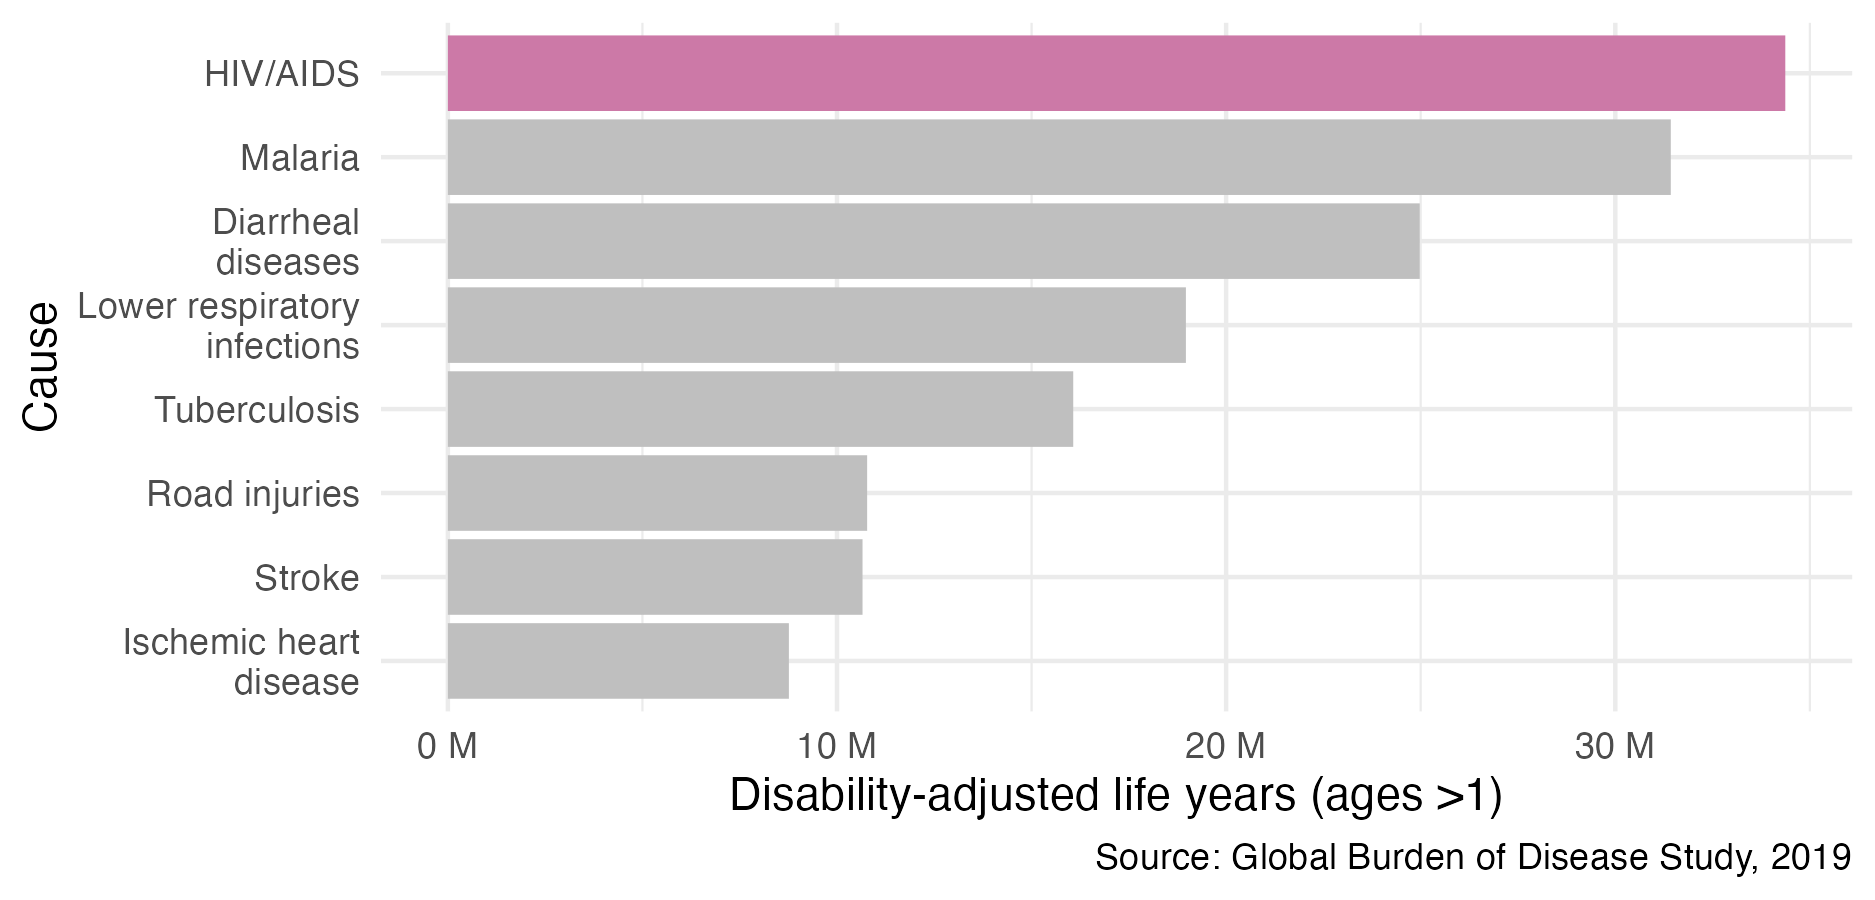
\includegraphics[width=0.95\linewidth]{figures/introduction/gbd} 

}

\caption{HIV/AIDS is the largest cause of annual DALYs among individuals aged \textgreater1 year in SSA \autocite{ihme2019}. One DALY represents the loss of the equivalent of one year of full health, and is calculated by the sum of years of life lost and years lost due to disability. The disability weights vary between 0 (full health) and 1 (death) depending on severity of the condition.}\label{fig:gbd}
\end{figure}

The real world questions are related to strategic information for planning the human immunodeficiency virus (HIV) epidemic response in sub-Saharan Africa (SSA).
Over 40 years since the beginning of the epidemic, HIV is the largest annual cause of disability adjusted life years (DALYs) in SSA among non-infants {[}\textcite{ihme2019}; Figure \ref{fig:gbd}{]}.
Quantification of the epidemic using statistics is an important part of the public health response.
Effective implementation of both HIV prevention and treatment requires strategic information.
However, producing suitable estimates of relevant indicators is challenging.

The data I use are recorded from national household surveys or routinely collected from healthcare facilities providing HIV services.
An important feature of these data are the location and the time at which each observation was recorded
While diverse, spatio-temporal data have distinctive commonalities which reoccur across settings.
As a result, the work in this thesis makes use of, and aspires to contribute to the development of, modelling techniques from spatio-temporal statistics.

Computation is an essential part of modern statistical practice.
Each project in this thesis, and the thesis itself, is accompanied by R \autocite{r} code, hosted on GitHub at \href{https://github.com/athowes}{\texttt{https://github.com/athowes}}.

\hypertarget{chapter-overview}{%
\section{Chapter overview}\label{chapter-overview}}

This thesis is structured (Figure \ref{fig:chapter-flowchart}) as follows:

\begin{itemize}
\tightlist
\item
  Chapter \ref{hiv-aids} provides an overview of the HIV/AIDS epidemic, and describing the challenges faced by disease surveillance efforts.
\item
  Chapter \ref{bayes-st} introduces the statistical concepts and notation used throughout the thesis, focusing on Bayesian modelling and computation, spatio-temporal statistics, and survey methods.
\item
  Chapter \ref{beyond-borders}: The prevailing model for spatial structure used in small-area estimation \autocite{besag1991bayesian} was intended to analyse a grid of pixels.
  In disease mapping, we work using the districts of a country, which are typically not a grid.
  I evaluated the practical consequences of this concern \autocite{howes2023beyond}.
\item
  Chapter \ref{multi-agyw}: Adolescent girls and young women are a demographic group at disproportionate risk of acquiring HIV infection.
  The Global AIDS Strategy recommends prioritising interventions on the basis of behaviour to prevent the most new infections using available resources.
  I estimated the size of behavioural risk groups across priority countries to enable implementation of this strategy, and assessed the potential benefits in terms of numbers of new infections prevented \autocite{howes2023spatio}.
  This work was included in the UNAIDS Global AIDS Update 2022 and 2023.
\item
  Chapter \ref{naomi-aghq}: The Naomi small-area estimation model \autocite{eaton2021naomi} is used by countries to estimate district-level HIV indicators.
  With this model in mind, I developed an approximate Bayesian inference method combining adaptive Gauss-Hermite quadrature with principal components analysis \autocite{howes2023fast}.
  I applied the method to data from Malawi, and analysed the consequences of inference method choice for policy relevant outcomes.
  Further, I open the door to a new class of fast, flexible, and accurate Bayesian inference algorithms.
\item
  Chapter \ref{conclusions}: Finally, I discuss avenues for future work, and my conclusions regarding the research, as well as its strengths and weaknesses.
\end{itemize}



\begin{figure}

{\centering 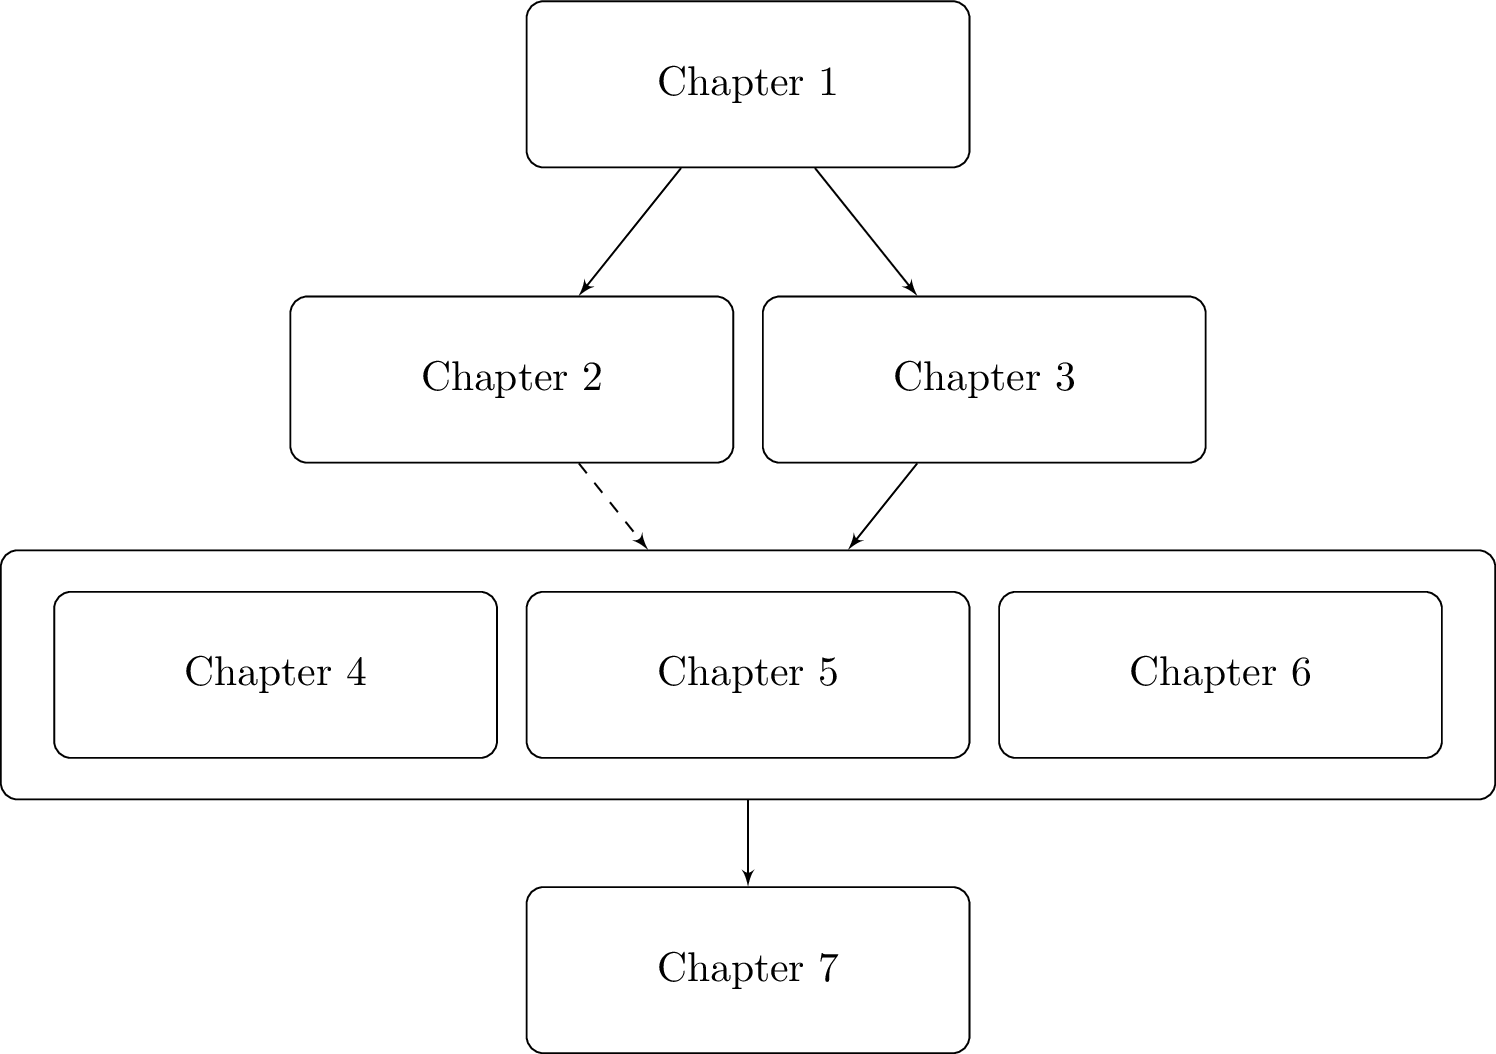
\includegraphics[width=0.95\linewidth]{figures/introduction/chapter-flowchart} 

}

\caption{Some chapters of the thesis should be read before others. Dashed lines represent recommended, but not required reading. Though chronological order is recommended, Chapters \ref{beyond-borders}, \ref{multi-agyw} and \ref{naomi-aghq} may be read in any order as they correspond to research projects which are for the most part separable.}\label{fig:chapter-flowchart}
\end{figure}

\hypertarget{hiv-aids}{%
\chapter{The HIV/AIDS epidemic}\label{hiv-aids}}

\adjustmtc
\markboth{The HIV/AIDS epidemic}{}

\hypertarget{background}{%
\section{Background}\label{background}}

HIV is a retrovirus which infects humans.
If untreated, HIV can develop into a more advanced stage known as acquired immunodeficiency syndrome (AIDS).
HIV primarily attacks a type of white blood cell vital for the function of the immune system.
As a result, AIDS is characterised by increased risk of developing opportunistic infections such as tuberculosis or \emph{Pneumocystis} pneumonias.

The first AIDS cases were reported in Los Angeles in the early 1980s \autocite{gottlieb1981pneumocystis,barre1983isolation}.
Since then, HIV has spread globally.
Transmission occurs by exposure to specific bodily fluids of an infected person.
The most common mode of transmission is via unprotected anal or vaginal sex, though transmission can also occur from a mother to her baby, or when drug injection equipment is shared.
Approximately 86 million people have become infected with HIV, and of those 40 million have died of AIDS-related causes.

An ongoing global and multifaceted effort has been made to respond to the epidemic.
The response has been shaped by local communities, civil society organisations, governments, research institutions, pharmaceutical companies, international agencies like the Joint United Nations Programme on HIV/AIDS (UNAIDS), and global health initiatives such like the President's Emergency Plan for AIDS Relief (PEPFAR) and the Global Fund to Fight AIDS, Tuberculosis, and Malaria (the Global Fund).
The investment of \$100 billion by PEPFAR, constituting the ``largest commitment by a single nation to address a single disease in history'' \autocite{pepfar2022}, is indicative of the scale of the response.



\begin{figure}

{\centering 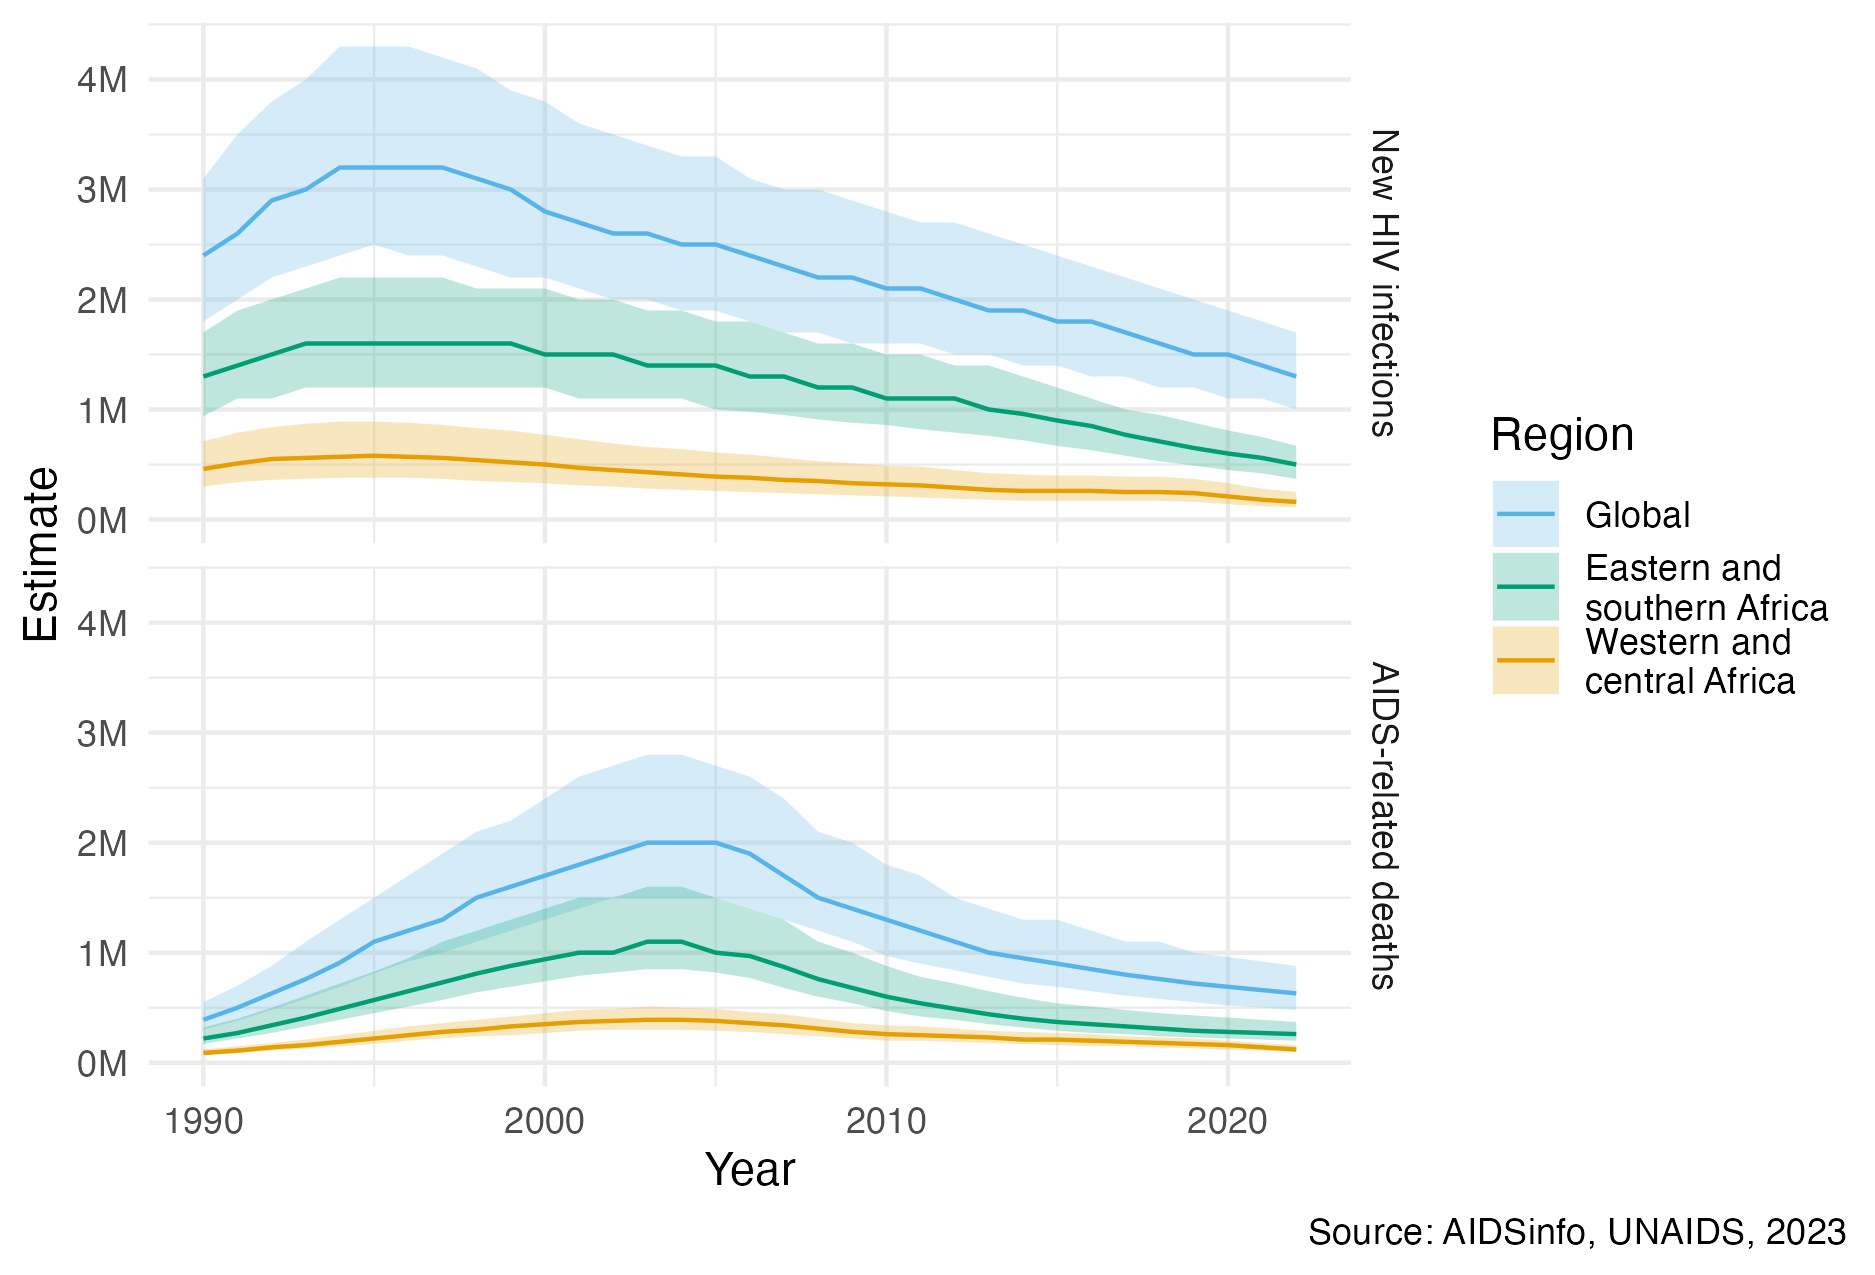
\includegraphics[width=0.95\linewidth]{figures/hiv-aids/overall-picture} 

}

\caption{Globally, yearly new HIV infections peaked in 1995, and have since decreased by 59\% and yearly AIDS-related deaths peaked in 2004, and have since decreased by 68\% \autocite{unaids2023aidsinfo}. Much of the disease burden is concentrated in eastern and southern Africa, as well as western and central Africa.}\label{fig:overall-picture}
\end{figure}

Implementation of HIV prevention and treatment has significantly reduced the number of new HIV infections and AIDS-related deaths per year since their peak (Figure \ref{fig:overall-picture}).
The most significant evidence-based interventions are:

\begin{itemize}
\tightlist
\item
  Condoms are an inexpensive and effective method for prevention of HIV and other sexually transmitted infections (STIs) such as \emph{Chlamydia trachomatis}, \emph{Neisseria gonorroeae}, syphilis, and \emph{Trichomonas vaginalis}.
  Condom usage has increased significantly since 1990, which is estimated to have averted 117 million new HIV infections \autocite{stover2021impact}.
  That said, there remain significant and difficult to close gaps in condom usage.
\item
  Antiretroviral therapy (ART) is a combination of drugs which stop the virus from replicating in the body.
  A person living with HIV who takes ART daily can live a full and healthy life, transforming what was once a terminal illness to a treatable chronic condition.
  Of the 39 million people living with HIV (PLHIV) in 2022, around 76\% were accessing ART.
  A staggering 21 million AIDS-related deaths are estimated to have been averted by ART \autocite{unaids2023global}.
  ART reduces the amount of virus in the blood and genital secretions.
  If the virus is undetectable then there is considerable evidence that it cannot be transmitted sexually \autocite{cohen2011prevention,broyles2023risk}.
  For this reason, in addition to providing life saving treatment, ART also operates as prevention.
  Particular efforts have been made to provide pregnant women with ART to reduce the chance of mother-to-child transmission (MTCT) \autocite{siegfried2011antiretrovirals}.
\item
  Voluntary medical male circumcision (VMMC) partially protects against female-to-male HIV acquisition.
  Three landmark randomised control trials \autocite{auvert2005randomized,gray2007male,bailey2007male} found complete surgical removal of the foreskin to result a reduction of HIV acquisition in men by 50-60\%.
  Based on this evidence, VMMC has been recommended since 2007 by the World Health Organization (WHO) and UNAIDS as a key HIV intervention in high-prevalence settings.
  Scale up of VMMC across 15 priority countries between 2008 and 2019 is estimated to have already averted 340 thousand new HIV infections, though the future number of new HIV infections averted is likely to be much higher.
\item
  Pre-exposure prophylaxis (PrEP) and post-exposure prophylaxis (PEP) are antiretrovial drugs which can be taken before and after exposure to prevent transmission.
  PrEP and PEP are more costly than some other prevention options, so primarily useful in high risk settings.
\end{itemize}

Though important progress had been made, there remains much more to do.
In 2022, 1.3 million people were newly infected with HIV and there were 630 thousand AIDS-related deaths, more than one every minute \autocite{unaids2022global}.
Bold fast-track targets have been set to accelerate the end of AIDS as global public health threat by 2030.
Renewed commitment is required to meet these targets in the context of disruption to HIV services caused by the COVID-19 pandemic and a shortfall in HIV funding \autocite{economist2023triple}.



\begin{figure}

{\centering 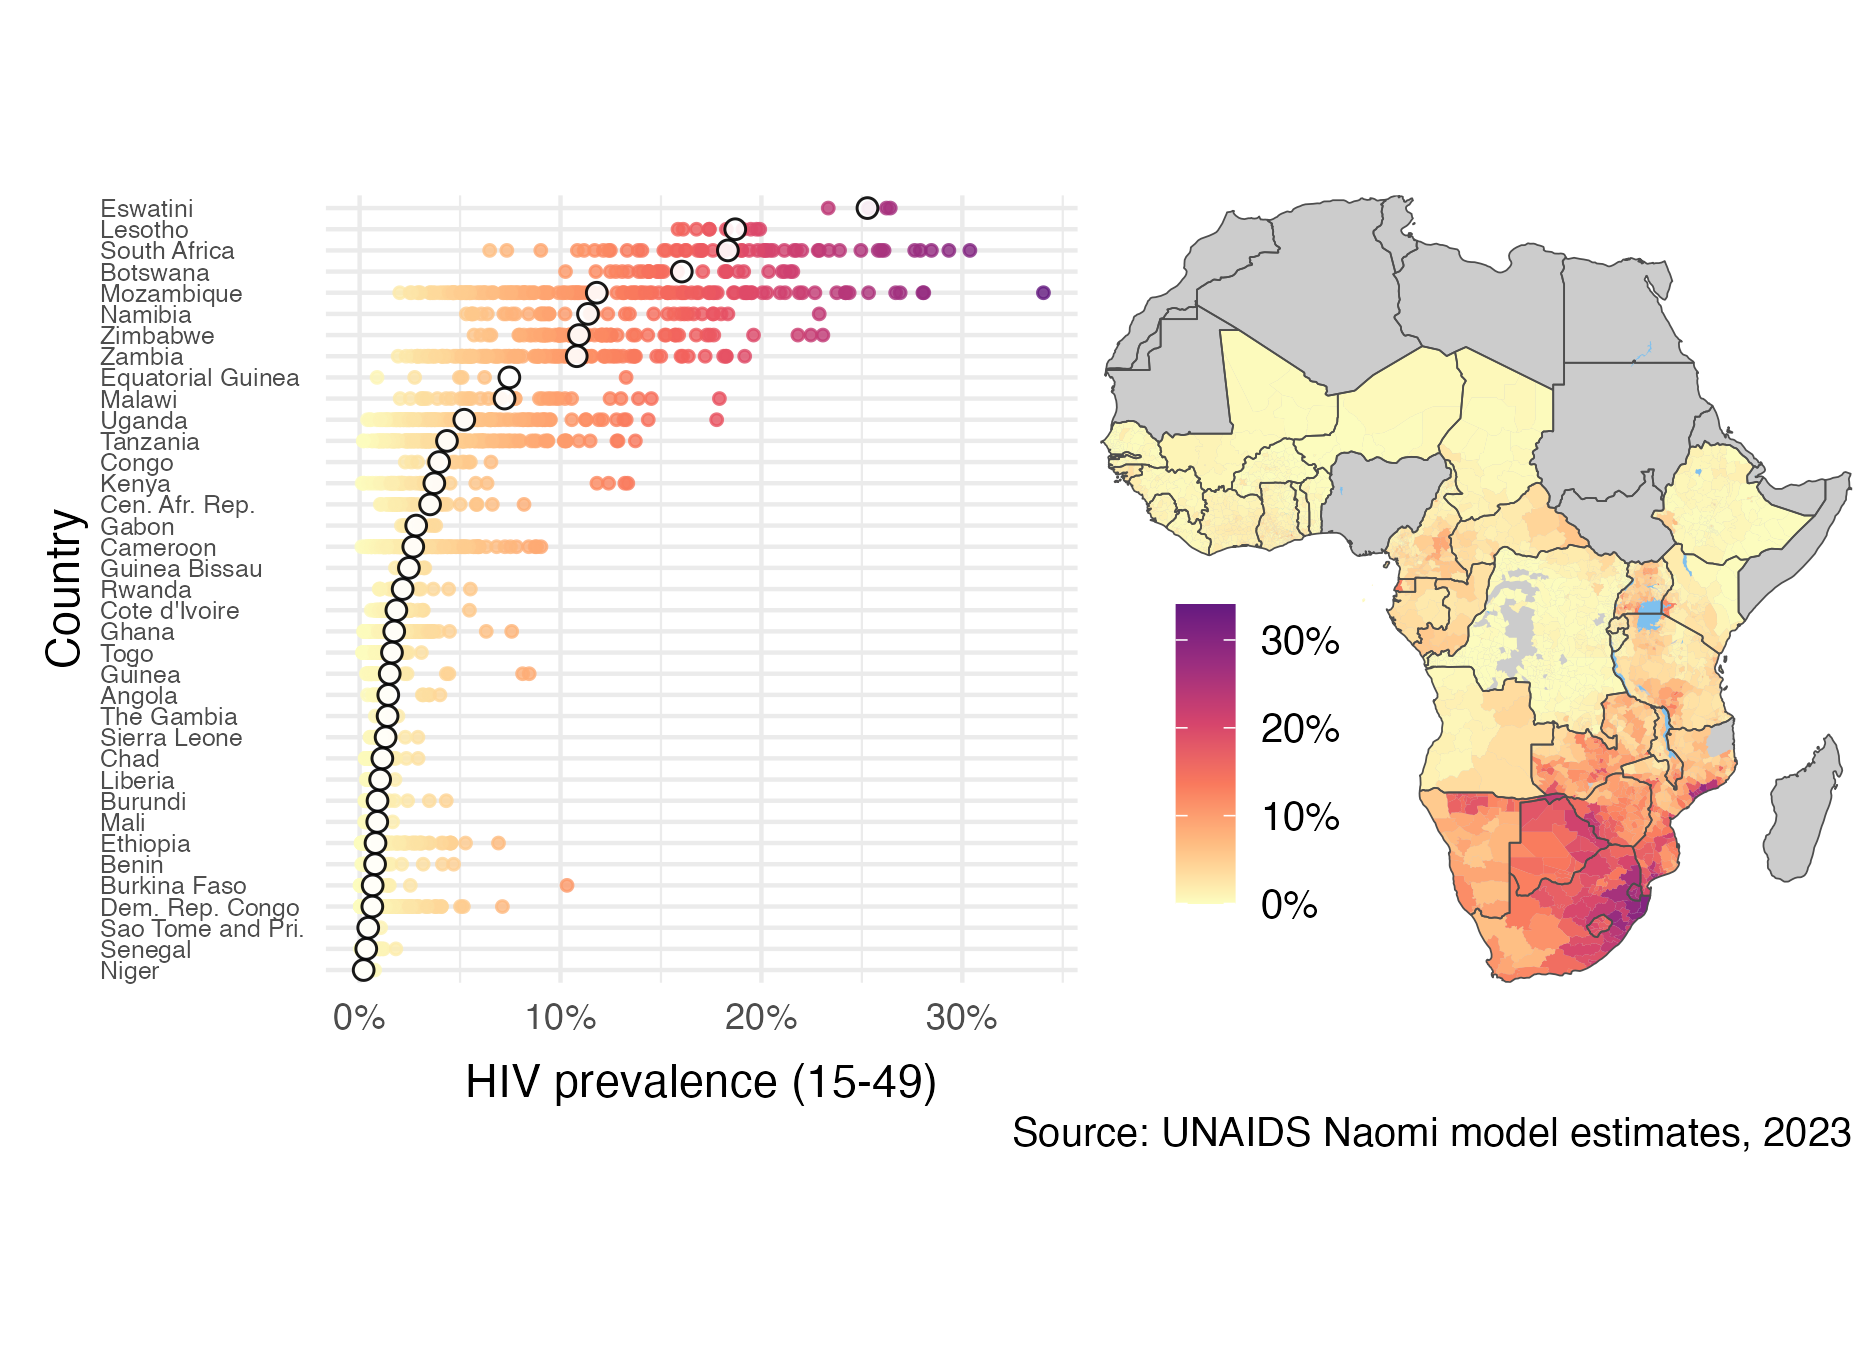
\includegraphics[width=0.95\linewidth]{figures/hiv-aids/naomi-continent} 

}

\caption{Adult (15-49) HIV prevalence varies substantially both within and between countries in SSA. These estimates from 2023 were generated by country teams using the Naomi small-area estimation model in a process supported by UNAIDS and are available from \textcite{unaids2023aidsinfo}. White filled points are country-level estimates, and coloured points are district-level estimates. Results from Nigeria were not published. Data collection in the Cabo Delgado province of Mozambique was disrupted by conflict. Obtaining results for the Democratic Republic of the Congo required removing some districts from the model. Country names are given by three-leter codes as published by the International Organization for Standardization (ISO).}\label{fig:naomi-continent}
\end{figure}

For available resources to have the greatest impact, it is important that HIV interventions are prioritised.
Under the precision public health paradigm, the right interventions should be provided to the right populations, in the right place, at the right time \autocite{khoury2016precision}.
Some interventions might be orders of magnitude more impactful than others \autocite{ord2013moral}.

Disease burden varies substantially across multiple spatial scales.
In some countries, the epidemic is concentrated in small populations, and national HIV prevalence is low.
In others, the epidemic is sustained by heterosexual transmission, and national HIV prevalence is higher (typically \textgreater1\%)
These two epidemic settings are described as concentrated and generalised respectively \autocite{tanser2014concentrated}.
Most of the countries severely affected by HIV are in sub-Saharan Africa (SSA).
It is estimated that 66\% of the 39 million PLHIV worldwide live in SSA.
Adult HIV prevalence (ages 15-49) is higher than 10\% (Figure \ref{fig:naomi-continent}) in some countries in southern Africa.
Just as there is variation between countries, there is variation within countries.
For example, adult HIV prevalence at the district municipality level in South Africa ranges from 6\% in Namakwa to 30\% in uMkhanyakude.

In all countries and contexts, some groups of people are at much higher risk than others.
Groups of people at increased risk of HIV infection are known as key populations (KPs).
Examples include men who have sex with men (MSM), female sex workers (FSW), people who inject drugs (PWID), and transgender people (TGP) \autocite{stevens2022key}.
KPs are often marginalised, and face legal and social barriers.
In concentrated settings, the majority of new HIV infections occur in KPs and their sexual partners.
In generalised settings like SSA, risk is more diffuse across the population.
For example, in SSA adolescent girls and young women (AGYW) are a large demographic group at increased risk of HIV infection \autocite{risher2021age,monod2023growing}, but not typically considered a KP.

\hypertarget{surveillance}{%
\section{HIV surveillance}\label{surveillance}}

HIV surveillance refers to the collection, analysis, interpretation and dissemination of data relating to HIV/AIDS.
Surveillance can used to track epidemic indicators, identify at-risk populations, find drivers of transmission, and evaluate the impact of prevention and treatment programs.
Important indicators include:

\begin{itemize}
\tightlist
\item
  \textbf{HIV prevalence} is the proportion \(\rho \in [0, 1]\) of the population who have HIV, typically written as a percentage.
  Both new infections and more PLHIV remaining alive by taking treatment increase HIV prevalence.
  As such, HIV prevalence should not be interpreted in isolation, and is primarily used indirectly to calculate other indicators.
  That said, in some circumstances when other indicators are difficult to estimate, HIV prevalence can be a useful proxy.
  The number of PLHIV is given by \(N\rho\), where \(N\) is the population size.
\item
  \textbf{HIV incidence} is the rate \(\lambda \in \mathbb{R}\) of new HIV infections, typically written as number of new infections per 1000 person years.
  HIV incidence can be specified in terms of the change in HIV prevalence over some time period \(\lambda = \Delta \rho / \Delta t\).
  Planning, delivery, and evaluation of prevention programming relies on estimates of HIV incidence.
  The number of new HIV infections is given by \(N (1 - \rho) \lambda\).
\item
  \textbf{ART coverage} is the proportion \(\alpha \in [0, 1]\) of PLHIV who are on ART, typically written as a percentage.
  Estimates of ART coverage play a direct role in the provision of treatment services.
  The number of people taking ART is given by \(N \rho \alpha\).
\end{itemize}

\hypertarget{data}{%
\subsection{Data}\label{data}}

What are the current data?
What are the current approaches to using the data?

\hypertarget{challenges}{%
\subsection{Challenges}\label{challenges}}

Obtaining reliable, timely estimates at an appropriate spatial resolution is challenging.
The most significant difficulties faced are:

\begin{enumerate}
\def\labelenumi{\arabic{enumi}.}
\tightlist
\item
  \textbf{Data sparsity}:
  Collection of data is costly and time consuming.
  As a result, limited direct data might be available for the particular time, location, and sub-population of interest.
  For example, in many countries the last conducted household survey is several years out of date.
\item
  \textbf{Missing data}:
  The sampling frame of a survey may not correspond to the target population.
  For example, many KPs are difficult to reach, and may be omitted from sampling frames.
  Individuals included on the sampling frame may choose not to respond.
  All surveys are subject to sampling error, as only a subset of the target population are sampled.
  Each of these issues can be characterised as being problems of missing data.
  I characterise missing data as referring to the shortfalls of any given study, and data sparsity as referring to limited availability of studies.
\item
  \textbf{Response and measurement biases}:
  Individuals may be hesitant to disclose their HIV status, or report higher risk behaviours, due to social desirability bias or a fear of discrimination or stigma.
  When available, biomarker data can be used to overcome under-reporting, but still may be subject to measurement errors.
\item
  \textbf{Denominators and demography}:
  Many indicators are rates or proportions, which rely on estimates of the population at risk in the denominator.
  Accurately estimating population denominators is itself a challenging task \autocite{tatem2017worldpop}.
  Taking a ratio of uncertain quantities amplifies uncertainty, but is rarely properly accounted for.
\item
  \textbf{Inconsistent data collection and reporting}:
  The types of data that are collected might vary across space and time.
  Reporting protocols or definitions can also change.
\item
  \textbf{Reliance on epidemiological parameters}:
  Indicators rely on estimates of epidemiological parameters such as rates of disease progression.
  These parameters are typically obtained from cohort studies and may not generalise to the setting of interest.
  Further, they are typically applied coarsely, and without proper accounting for uncertainty.
\end{enumerate}

\hypertarget{statistical-approaches}{%
\subsection{Statistical approaches}\label{statistical-approaches}}

The challenges above make direct interpretation of the data often misleading or impossible.
Careful statistical modelling is required to overcome these limitations as best as possible.

\begin{enumerate}
\def\labelenumi{\arabic{enumi}.}
\tightlist
\item
  \textbf{Borrowing information}:
  When little direct data are available, data judged to be indirectly related can be used to help improve estimation.
  For example, if limited data are available for individuals of a certain age is a particular country, it is likely reasonable to make use of data for individuals of a similar age in that country.
  As well as over age groups, information can be borrowed between and within countries, and across times.
\item
  \textbf{Evidence synthesis}:
  Multiple sources of evidence can be combined to overcome the limitations of any one data source.
  For example, infrequently run household surveys can be complemented by up to date programmatic data.
\item
  \textbf{Expert guidance}:
  Expert epidemiological, demographic, and local stakeholder guidance can be used to improve estimates.
  Ensuring the quality of any data used in the estimation process is essential.
\item
  \textbf{Uncertainty quantification}:
\end{enumerate}

\hypertarget{future-directions}{%
\subsection{Future directions}\label{future-directions}}

Aims for HIV response going forward, and the surveillance capabilities needed to meet them:

\begin{enumerate}
\def\labelenumi{\arabic{enumi}.}
\tightlist
\item
  \textbf{Greater reliance on routine health system data}:
  It is not recommended to include HIV testing in nationally representative household surveys in low (\textless2\%) HIV prevalence settings \autocite{world2005guidelines}. Patient-level HIV data systems \autocite{world2017consolidated} and case-based surveillance (CBS). Integration of HIV services with other health programs and strengthening of health systems.
\end{enumerate}

\hypertarget{bayes-st}{%
\chapter{Bayesian spatio-temporal statistics}\label{bayes-st}}

\adjustmtc
\markboth{Bayesian spatio-temporal statistics}{}

\hypertarget{bayesian-statistics}{%
\section{Bayesian statistics}\label{bayesian-statistics}}

Bayesian statistics is a mathematical paradigm for learning information from data.
It is especially well suited to facing the challenges posed by Section \ref{surveillance} because it allows for principled and flexible integration of prior domain knowledge.
Additionally, uncertainty over all unknown quantities is handled as an integral part of the Bayesian paradigm.
This section provides a brief and opinionated overview.
For a more complete introduction, I recommend \textcite{gelman2013bayesian}, \textcite{mcelreath2020statistical} or \textcite{gelman2020bayesian}.

\hypertarget{bayesian-modelling}{%
\subsection{Bayesian modelling}\label{bayesian-modelling}}

The Bayesian approach to data analysis is based on construction of a probability model for the observed data \(\mathbf{y} = (y_1, \ldots, y_n)\) together with parameters \(\boldsymbol{\mathbf{\phi}} = (\phi_1, \ldots, \phi_d)\).
Choice of the particular parameters used depends upon the requirements of the analysis.
All quantities are assumed to be random variables, and the model is written as \(p(\mathbf{y}, \boldsymbol{\mathbf{\phi}})\), where \(p(\cdot)\) denotes a probability distribution.
Subsequent calculations are based on manipulation of this model using probability theory.

Models can be most naturally constructed from two parts, known respectively as the likelihood \(p(\mathbf{y} \, | \, \boldsymbol{\mathbf{\phi}})\) and the prior distribution \(p(\boldsymbol{\mathbf{\phi}})\).
The joint distribution is obtained by the product \(p(\mathbf{y}, \boldsymbol{\mathbf{\phi}}) = p(\mathbf{y} \, | \, \boldsymbol{\mathbf{\phi}}) p(\boldsymbol{\mathbf{\phi}})\).
The likelihood, as a function of \(\boldsymbol{\mathbf{\phi}}\) with \(\mathbf{y}\) fixed, reflects the probability of observing the data when the value of the parameters is \(\boldsymbol{\mathbf{\phi}}\).
The prior distribution encapsulates beliefs about the parameters \(\boldsymbol{\mathbf{\phi}}\) before the data are observed.

Recommendations for specifying prior distributions vary.
The extent to which subjective information should be incorporated into the prior distribution, and in doing so influence the posterior distribution, is a central topic of discussion.
Proponents of the objective Bayesian paradigm \autocite{berger2006case} put forward that the prior distribution should be non-informative, so as not to introduce subjectivity into the analysis.
That said, we shall see in Section \ref{hierarchical-lgm-elgm} that the distinction between likelihood and prior distribution can be unclear.
As such, it may be argued that issues of subjectivity are not unique to the prior distribution, and ultimately the challenge of specifying the data generating process is better thought of more holistically.

The probability model can be simulated from to obtain samples \((\mathbf{y}, \boldsymbol{\mathbf{\phi}}) \sim p(\mathbf{y}, \boldsymbol{\mathbf{\phi}})\).
If the samples of \(\mathbf{y}\) differ too greatly from what the analyst would expect, then the model does not capture their prior scientific understanding of the data.
Models which do not produce plausible samples can be refined.
Checks of this kind {[}\textcite{gelman2013bayesian}; Chapter 6{]} can be used to help iteratively build models, adding complexity gradually as required.

\hypertarget{bayesian-computation}{%
\subsection{Bayesian computation}\label{bayesian-computation}}



\begin{figure}

{\centering 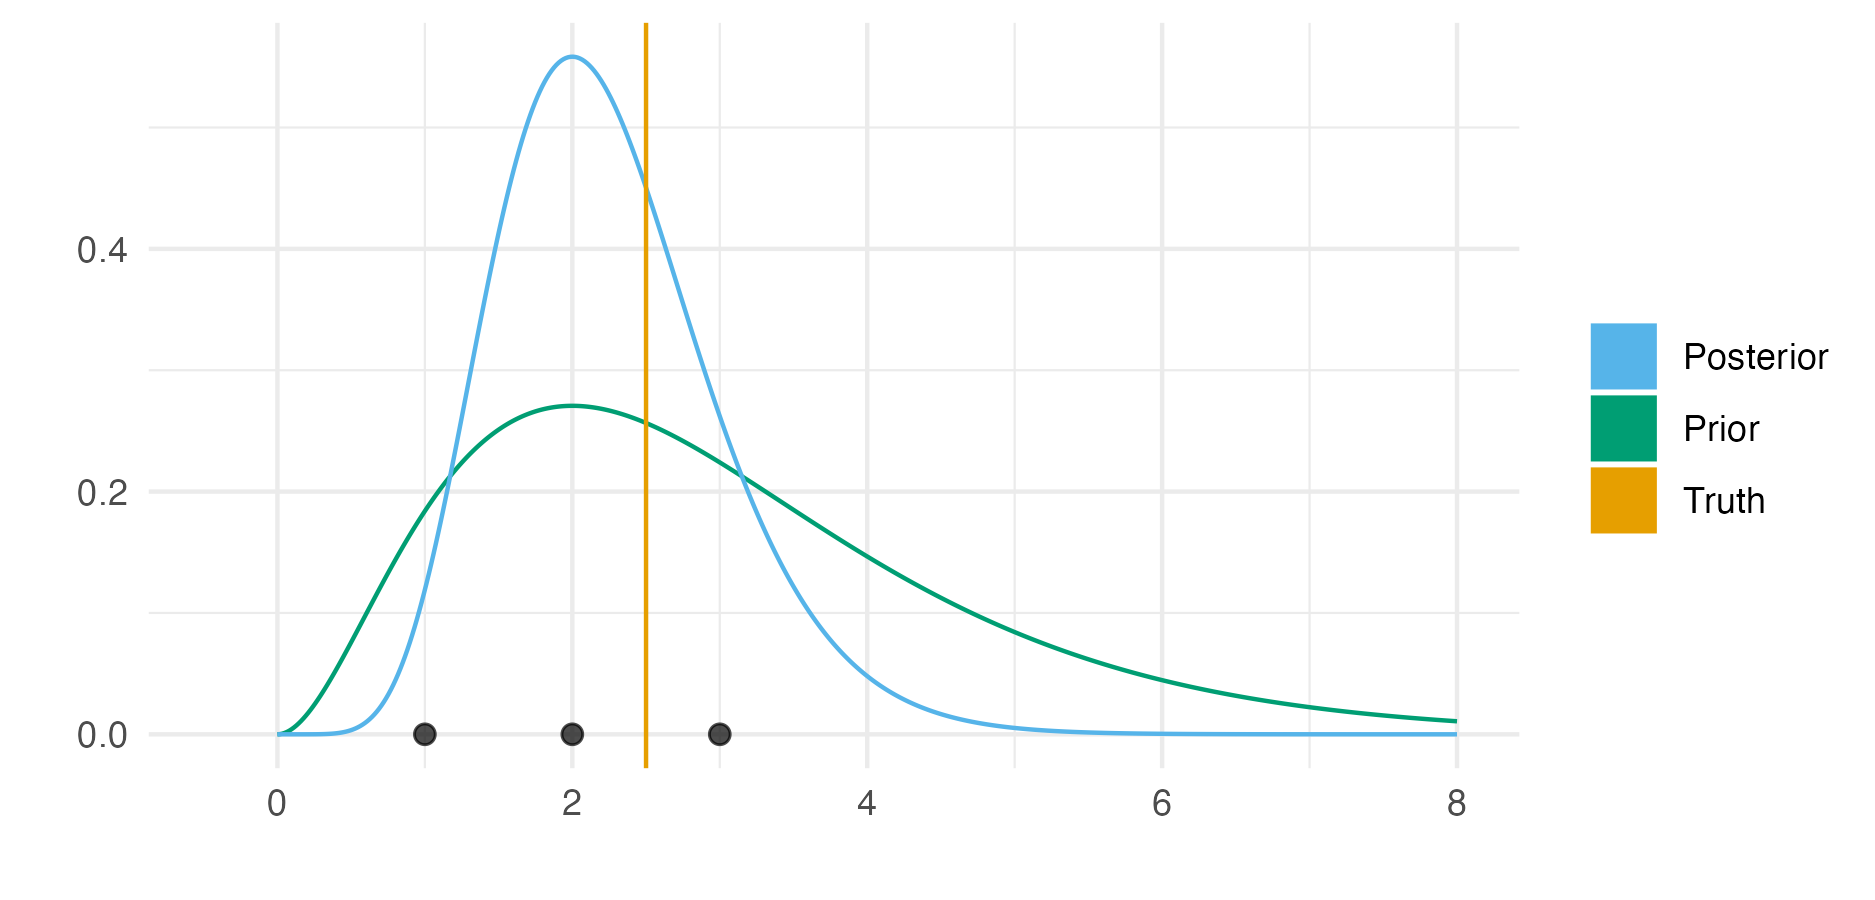
\includegraphics[width=0.95\linewidth]{figures/bayesian/conjugate} 

}

\caption{An example of Bayesian modelling and computation for a simple one parameter model. Here the likelihood is \(y_i \sim \text{Poisson}(\phi)\) for \(i = 1, 2, 3\) and prior distribution on the rate parameter is \(\phi \sim \text{Gamma}(3, 1)\). I simulated observed data \(\mathbf{y} = (1, 2, 3)\) from the distribution \(\text{Poisson}(2.5)\). As such, the true data generating process is within the space of models being considered (This situation is sometimes known \autocite{bernardo2001bayesian} as the \(\mathcal{M}\)-closed world, in contrast to the \(\mathcal{M}\)-open world where the model is said to be misspecified .) Furthermore, the posterior distribution is available in closed form as \(\text{Gamma}(9, 4)\). This is because the posterior distribution is in the same family of probability distributions as the prior distribution, and the model is described as being conjugate. Conjugate models are often used because of their convenience. Though other models may be more suitable, they will typically be more computationally demanding. In this situation, which is typical, the posterior distribution is more tightly peaked than the prior distribution.}\label{fig:conjugate}
\end{figure}

The primary goal in a Bayesian analysis is to obtain the posterior distribution \(p(\boldsymbol{\mathbf{\phi}} \, | \, \mathbf{y})\).
This distribution encapsulates probabilistic beliefs about the parameters given the observed data, and has a central role in use of the analysis for decision making.
Using the eponymous Bayes' theorem, the posterior distribution is obtained by
\begin{equation}
p(\boldsymbol{\mathbf{\phi}} \, | \, \mathbf{y}) = = \frac{p(\mathbf{y}, \boldsymbol{\mathbf{\phi}})}{p(\mathbf{y})} = \frac{p(\mathbf{y} \, | \, \boldsymbol{\mathbf{\phi}}) p(\boldsymbol{\mathbf{\phi}})}{p(\mathbf{y})}. \label{eq:posterior}
\end{equation}

Unfortunately, most of the time it is intractable to calculate the posterior distribution analytically.
This is because of the potentially high-dimensional integral
\begin{equation}
p(\mathbf{y}) = \int p(\mathbf{y}, \boldsymbol{\mathbf{\phi}}) \text{d}\boldsymbol{\mathbf{\phi}}
\end{equation}
in the denominator of Equation \eqref{eq:posterior}.
The evidence \(p(\mathbf{y})\) quantifies the probability of obtaining the data under the model, and\ldots{} TODO.
As such, although it is easy to evaluate a quantity proportional to the posterior distribution
\begin{equation}
p(\boldsymbol{\mathbf{\phi}} \, | \, \mathbf{y}) \propto p(\mathbf{y} \, | \, \boldsymbol{\mathbf{\phi}}) p(\boldsymbol{\mathbf{\phi}}),
\end{equation}
it is typically difficult to evaluate the posterior distribution itself.

The difficulty in performing Bayesian inference in general may be thought of as analogous to the difficulty in calculating integrals.
As with integration, in some cases closed form analytic solutions are available.
Figure \ref{fig:conjugate} illustrates one such case, where the prior distribution and posterior distribution are in the same family of probability distributions.
For the more general case where no analytic solution is available, computational methods have been developed to approximate the posterior distribution \autocite{martin2023computing}.
These methods may broadly be divided into Monte Carlo algorithms, and deterministic approximations.

\hypertarget{monte-carlo-algorithms}{%
\subsubsection{Monte Carlo algorithms}\label{monte-carlo-algorithms}}

Monte Carlo algorithms \autocite{robert2005monte} aim to generate samples from the posterior distribution
\begin{equation}
\boldsymbol{\mathbf{\phi}}_i \sim p(\boldsymbol{\mathbf{\phi}} \, | \, \mathbf{y}), \quad i \in 1, \ldots M.
\end{equation}
These samples may be used in any future computations involving functions of the posterior distribution.
For example, if \(G = G(\boldsymbol{\mathbf{\phi}})\) then the expectation of \(G\) with respect to the posterior distribution can be approximated by
\begin{equation}
\mathbb{E}(G \, | \, \mathbf{y}) = \int G(\boldsymbol{\mathbf{\phi}}) p(\boldsymbol{\mathbf{\phi}} \, | \, \mathbf{y}) \text{d} \boldsymbol{\mathbf{\phi}} \approx \frac{1}{M} \sum_{i = 1}^M G(\boldsymbol{\mathbf{\phi}}_i).
\end{equation}
Most quantities of interest can be cast as posterior expectations.

Markov chain Monte Carlo (MCMC) methods \autocite{roberts2004general} are the most popular class of sampling algorithms.
Using MCMC, samples are generated from by simulating from an ergodic Markov chain with the posterior distribution as its stationary distribution.
The Metropolis-Hastings {[}MH; \textcite{metropolis1953equation}; \textcite{hastings1970monte}{]} algorithm uses a proposal distribution \(q(\boldsymbol{\mathbf{\phi}}_{i + 1} \, | \, \boldsymbol{\mathbf{\phi}}_i)\) to generate candidate parameters for the next step in the Markov chain.
Many MCMC algorithms, including the Gibbs sampler, are special cases of MH.

Other notable classes of sampling algorithms include importance sampling (IS) methods, in which the samples are weighted, and sequential Monte Carlo {[}SMC; \textcite{chopin2020introduction}{]} methods based on sampling from a sequence of distributions.
Though these methods have found applications in specific domains, MCMC is more widely used because of its generality and theoretical reliability.

In this thesis, I use the No-U-Turn sampler {[}NUTS; \textcite{hoffman2014no}{]}, a Hamiltonian Monte Carlo {[}HMC; \textcite{duane1987hybrid}; \textcite{neal2011mcmc}{]} algorithm, as implemented in the Stan \autocite{carpenter2017stan} probabilistic programming language (PPL).
HMC uses derivatives of the posterior distribution to generate efficient Metropolis-Hastings proposal distributions based on Hamiltonian dynamics.
NUTS automatically adapts the tuning parameters of HMC based local properties of the posterior distribution.
Though not a one-size-fits-all solution, NUTS has been shown empirically to be a good choice for sampling from a range of posterior distributions.

After running an MCMC sampler, it is important to check diagnostics to assess accuracy and evaluate convergence.
Panel B of Figure \ref{fig:stan} shows a traceplot for a Markov chain which has converged.



\begin{figure}

{\centering 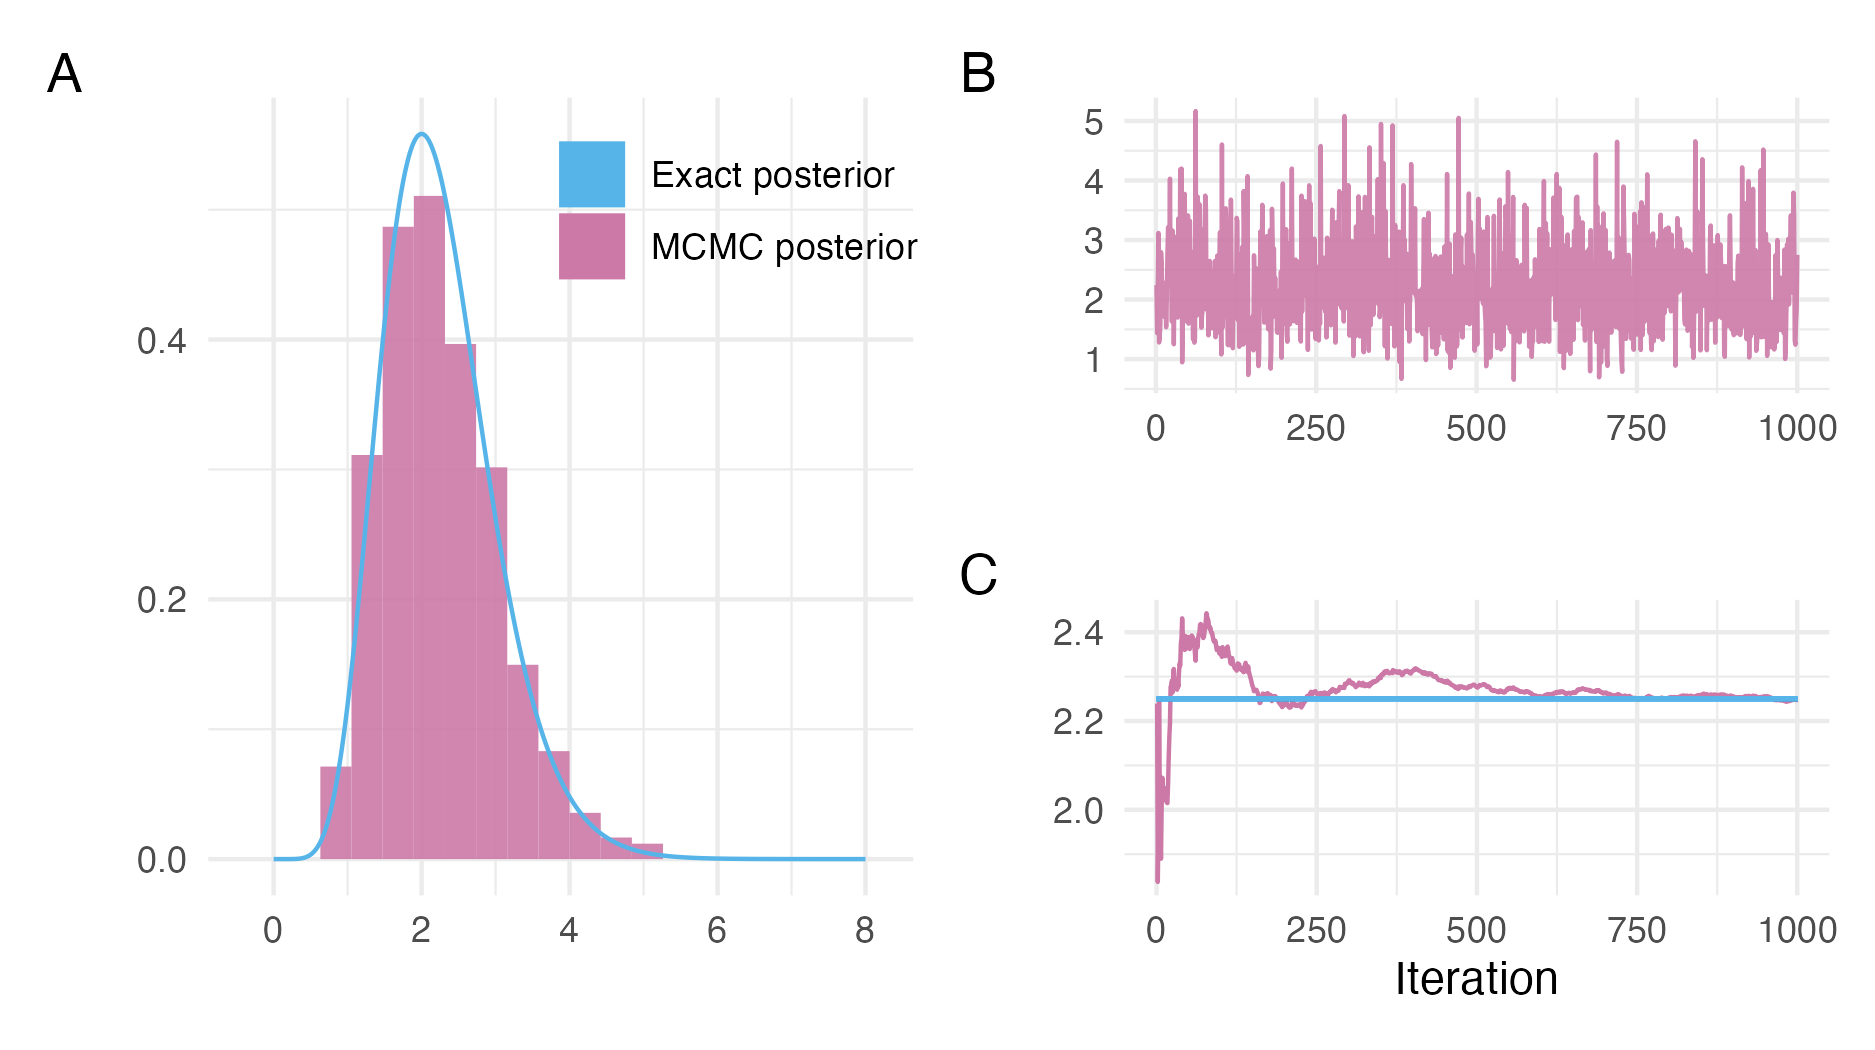
\includegraphics[width=0.95\linewidth]{figures/bayesian/stan} 

}

\caption{NUTS can be used to sample from the posterior distribution in the example of Figure \ref{fig:conjugate}. Panel A shows a histogram of the NUTS samples as compared to the true posterior. Panel B shows a traceplot. Panel C shows the convergence of the empirical posterior mean to the true value.}\label{fig:stan}
\end{figure}

\hypertarget{deterministic-approximations}{%
\subsubsection{Deterministic approximations}\label{deterministic-approximations}}

In variational inference {[}VI; \textcite{blei2017variational}{]} the approximate posterior distribution is assumed to belong to a particular family of functions.
Optimisation algorithms are used to choose the best member of that family, typically by minimising the Kullback-Leibler divergence to the posterior distribution.
VI is typically faster than Monte Carlo methods, especially for large datasets or models.
However, it lacks theoretical guarantees and is known to often inaccurately estimate posterior variances \autocite{giordano2018covariances}.
Developing diagnostics to evaluate the accuracy of VI is an important area of ongoing research \autocite{yao2018yes}.
The expectation maximisation {[}EM; \textcite{dempster1977maximum}{]} and expectation propagation {[}EP; \textcite{minka2001expectation}{]} algorithms are closely related to VI.

Need to talk about:
Laplace approximation.
Quadrature.
Integrated nested Laplace approximation.
Unsure how much detail to go into here given that these approximations are the subject of Chapter \ref{naomi-aghq}.

\hypertarget{interplay-between-modelling-and-computation}{%
\subsection{Interplay between modelling and computation}\label{interplay-between-modelling-and-computation}}

Modern computational techniques and software like PPLs have succeeded in abstracting away calculation of the posterior distribution from the analyst for many models.
However, computation remains intractable in the majority of cases.
As such, the analyst need not only to be concerned with choosing a model suitable for the data, but also choosing a model for which the posterior distribution is tractable in reasonable time.
As such, there is an important interplay between modelling and computation, wherein models are bound by the limits of computation.
As computation improves, the space of models available to the analyst expands.

\hypertarget{spatio-temporal-statistics}{%
\section{Spatio-temporal statistics}\label{spatio-temporal-statistics}}

Spatio-temporal statistics \autocite{cressie2015statistics} concerns observations which are indexed by spatial or temporal location.
In doing so, it unites the fields of spatial statistics \autocite{bivand2008applied} and time series analysis \autocite{shumway2017time}.

\hypertarget{properties-of-spatio-temporal-data}{%
\subsection{Properties of spatio-temporal data}\label{properties-of-spatio-temporal-data}}



\begin{figure}

{\centering 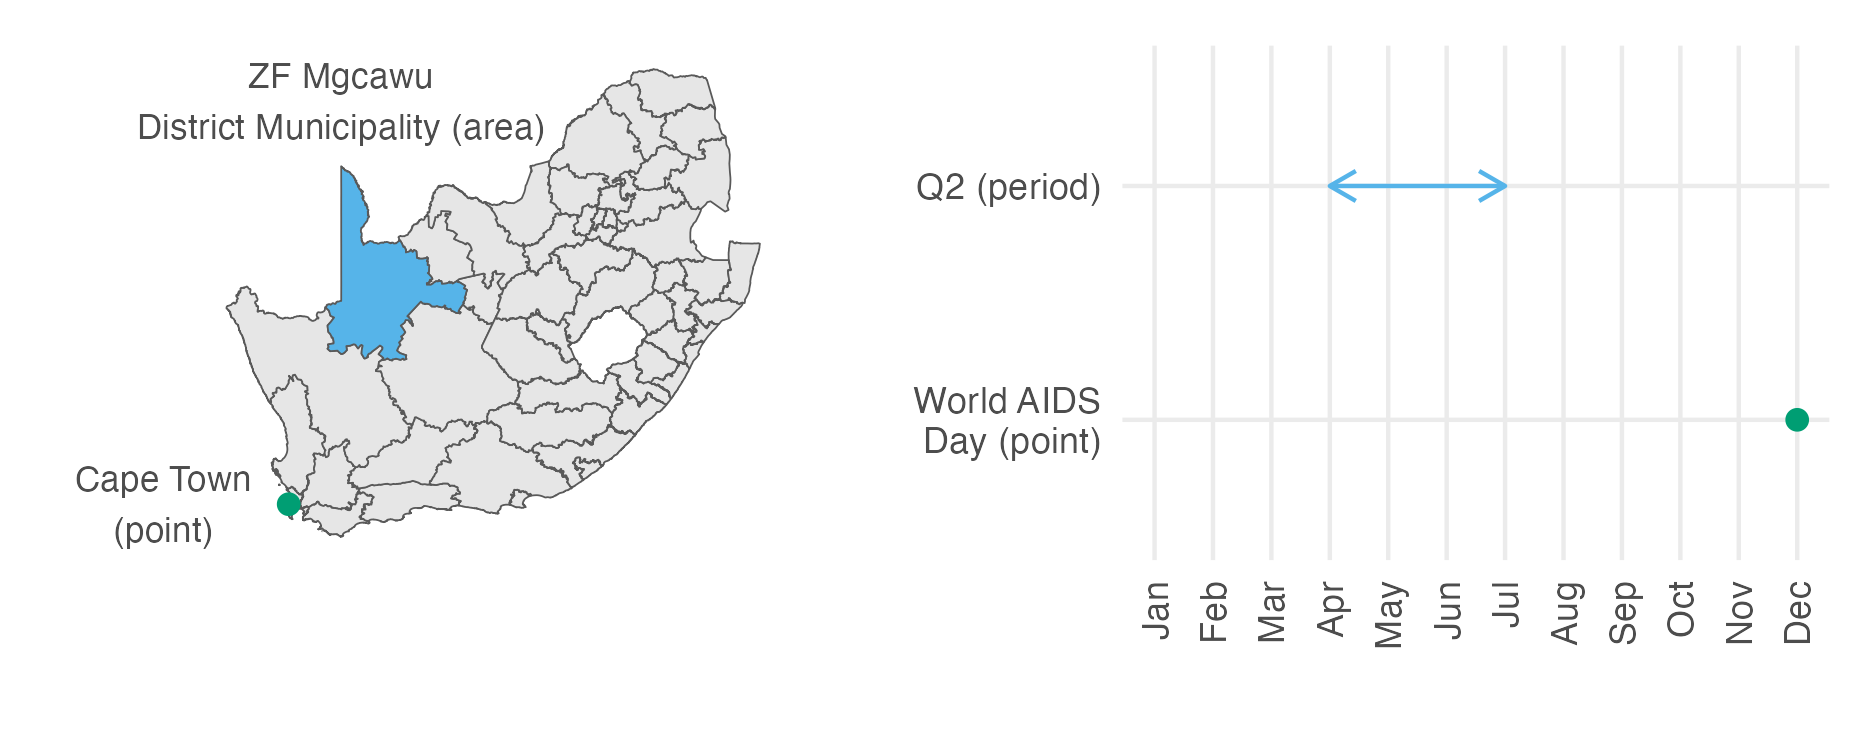
\includegraphics[width=0.95\linewidth]{figures/bayesian/st} 

}

\caption{The spatial location of Cape Town in South Africa could be considered a point. The ZF Mgcawu District Municipality on the other hand is an example of an area. World AIDS Day, designated on the 1st of December every year, could be considered a point in time. The second fiscal quarter, running through April, May and June, and denoted by Q2 represents a period of time. (In reality, both Cape Town and World AIDS Day are areas, rather than true point locations. Instances of infinitesimal point locations in everyday life are rare.)}\label{fig:st}
\end{figure}

Spatio-temporal data have some important properties:

\begin{enumerate}
\def\labelenumi{\arabic{enumi}.}
\item
  \textbf{Covariance structure}:
  According to Tobler's first law of geography ``everything is related to everything else, but near things are more related than distant things'' \autocite{tobler1970computer}.
  In ``The Design of Experiments'' \textcite{fisher1936design} observed that neighbouring crops were more likely to have similar yields than those far apart.
  This law can be formalised using spatial covariance functions.
  Spatial covariance functions are called isotropic when they apply equally in all directions, and stationary when they are invariant over space.

  As well as space, an Tobler's first law applies to time.
  Observations made close together in time tend to be similar.
  Temporal covariance structures are often periodic.

  The space-time covariance structure \autocite{porcu202130} is said to be separable when it can be factorised as a product of individual spatial and temporal covariances, and nonseparable when it can't.
  A separable space-time covariance could have spatial and temporal components which are either independent and identically distributed (IID) or structured \autocite{knorr2000bayesian}.

  Because of their covariance structure, spatio-temporal data are not IID.
  Only one observation of a spatio-temporal process is realised.
\item
  \textbf{Scales}:
  In this thesis I assume that the spatial study region \(\mathcal{S} \subseteq \mathbb{R}^2\) has two dimensions, corresponding to latitude and longitude.
  Observations may be associated to a point \(s \in \mathcal{S}\) or area \(A \subseteq \mathcal{S}\) in the study region.
  The temporal study period \(\mathcal{T} \subseteq \mathbb{R}\) can more generally be assumed to be one dimensional.
  Together with time only moving forward, this feature is what distinguishes time from space.
  As with space, observations may be associated to a point \(t \in \mathcal{T}\) or period of time \(T \subseteq \mathcal{T}\).
  Figure \ref{fig:st} illustrates both types of observation for space and time.

  As such, spatio-temporal observations can be made at various possible scales.
  Sometimes, we may want to model data at a scale it was not observed at.
  This is known as the change-of-support problem \autocite{gelfand2001change} and includes as special cases the problems of downscaling, upscaling, and dealing with so-called misaligned data.
  Closely related is the problem of wanting to jointly model data at different scales simultaneously.
\item
  \textbf{Size}:
  Data with both spatial and temporal dimensions are often large, making storage and operations on spatio-temporal data potentially difficult.
  Furthermore, models for spatio-temporal data typically require many parameters.
  Whereas large IID data can be modelled using a small number of parameters, each observation in a spatio-temporal dataset may need to be characterised by its own parameters.
  Large data combined with large models make Bayesian inference challenging.
\end{enumerate}

\hypertarget{small-area-estimation}{%
\subsection{Small-area estimation}\label{small-area-estimation}}

Data always has a cost to collect.
This cost can be significant, especially for data relating to people where collection is difficult to automate.
As a result, given the large number of possible locations in space and time, often no or limited direct observations may be available for any given space-time location.
Direct estimates of indicators of interest are either impossible or inaccurate in this setting.

Small-area estimation {[}SAE; \textcite{pfeffermann2013new}{]} methods aim to overcome the limitations of small data by sharing information.
In the spatio-temporal setting sharing of information occurs across space and time.
The fact that observations in one spatio-temporal location are correlated with those at another can be used to improve estimates.
Figures \ref{fig:zmb-maps} and \ref{fig:zmb-scatter} illustrate the unreliability of direct estimates from small sample sizes, and the way in which a spatial model may be used to overcome this limiation.

More generally, SAE methods are useful when data are limited for subpopulations of interest.
These subpopulations could be generated by spatio-temporal variables, as well as by other variables such as demographics.
Just as we expect there to be spatio-temporal correlation structure, we also can expect there to be demographic correlation structure.
Those of the same sex are more likely to be similar, as are those of similar ages or socioeconomic strata.



\begin{figure}

{\centering 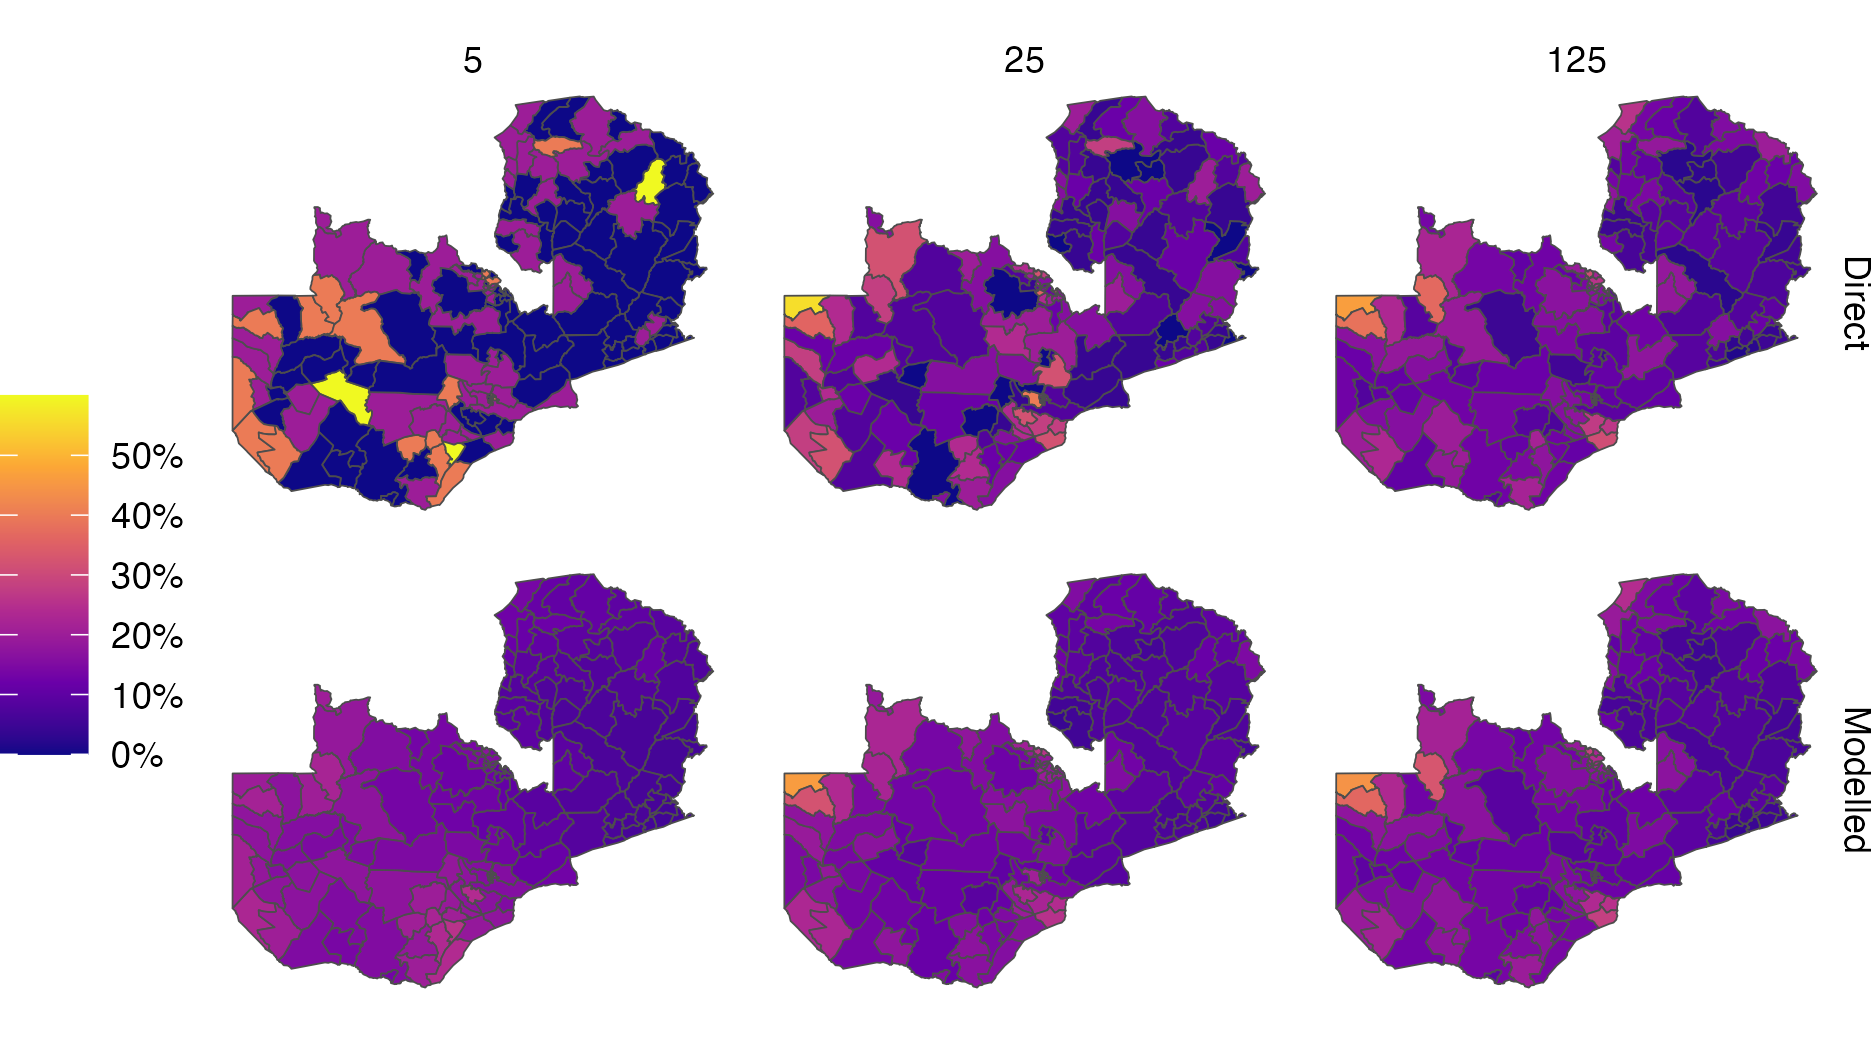
\includegraphics[width=0.95\linewidth]{figures/bayesian/zmb-maps} 

}

\caption{Simulation of a simple random sample \(y_i \sim \text{Bin}(m, p_i)\) with varying sample size (\(m = 5, 25, 125\)) in each of the \(i = 1, \ldots, 156\) constituencies of Zambia. Direct estimates were obtained by the ratio \(y_i / m\). Modelled estimates were obtained using a logistic regression with linear predictor given by an intercept and a spatial random effect. HIV estimates for Zambia have previously been generated at the district-level, comprising 116 spatial units. Moving forward, there is interest in generating estimates at the higher-resolution constituency level, as program planning is devolved locally. This figure is adapted from a presentation I gave for the Zambia HIV Estimates Technical Working Group, available from \href{https://github.com/athowes/zambia-unaids}{\texttt{https://github.com/athowes/zambia-unaids}}.}\label{fig:zmb-maps}
\end{figure}



\begin{figure}

{\centering 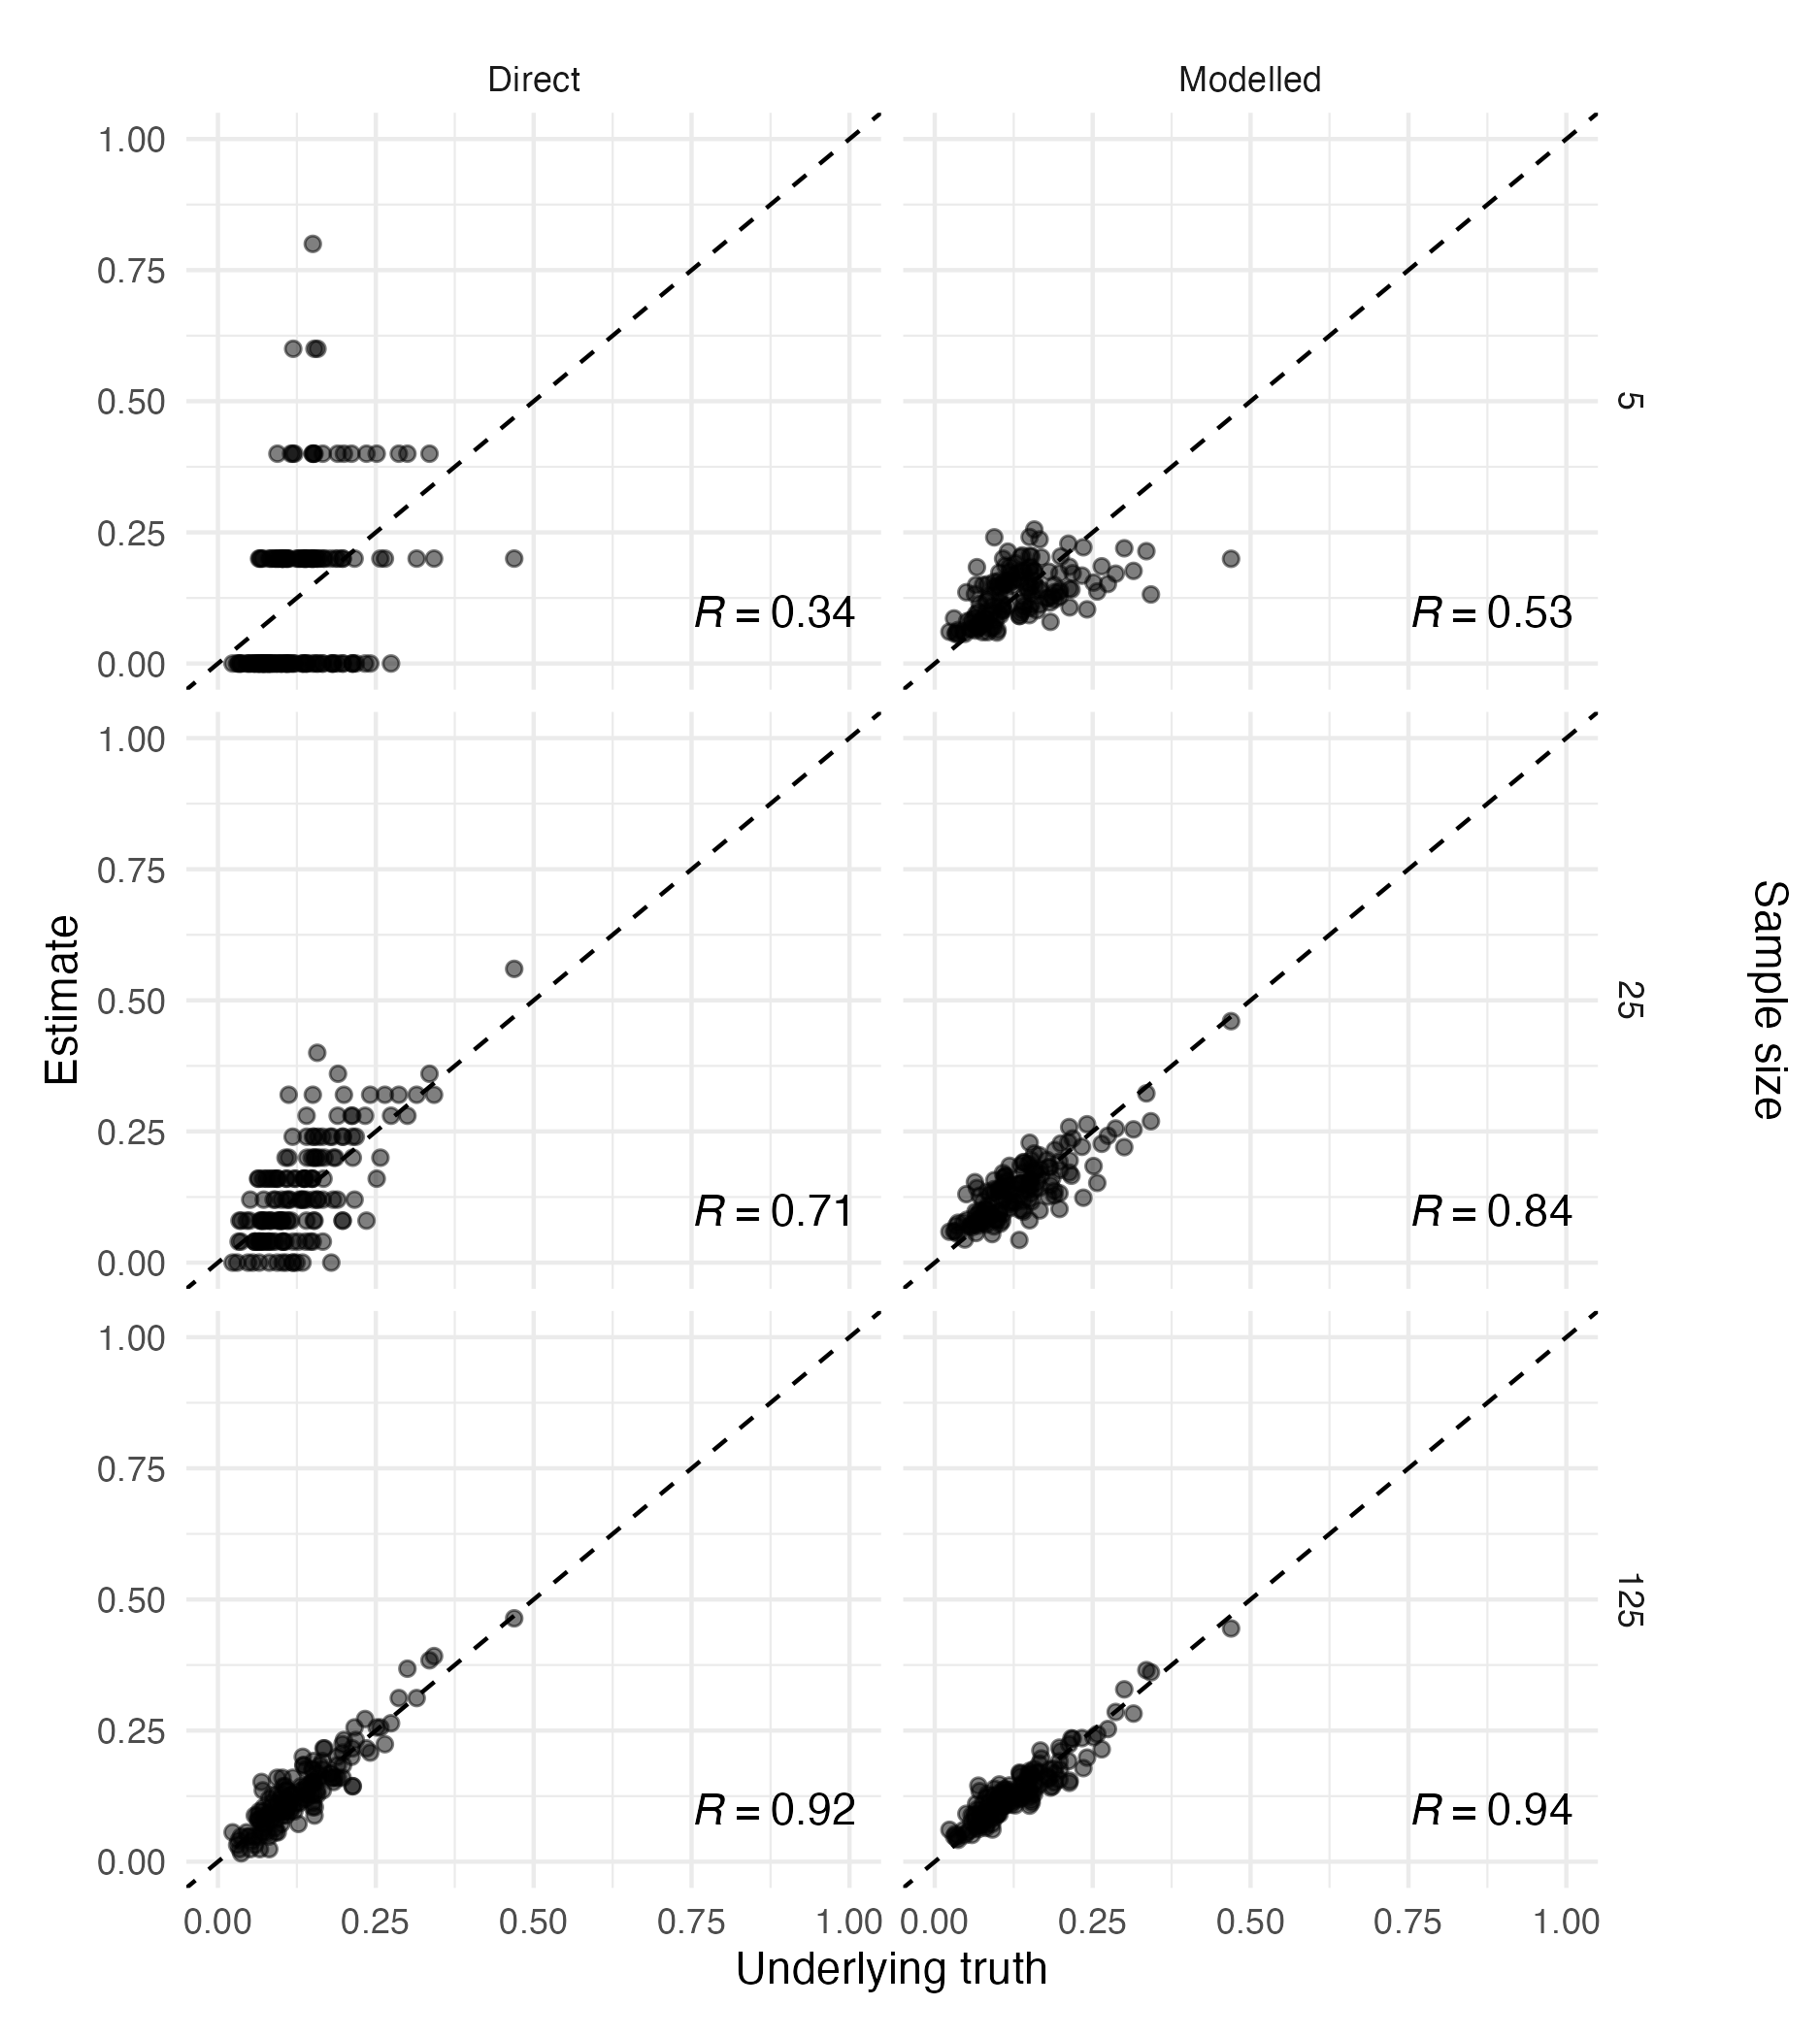
\includegraphics[width=0.95\linewidth]{figures/bayesian/zmb-scatter} 

}

\caption{The setting of this figure matches that of Figure \ref{fig:zmb-maps}. Estimates from surveys with higher sample size have higher Pearson correlation coefficient \(R\) with the underlying truth. For a fixed sample size, correlation can be improved by using modelled estimates to borrow information across spatial units, rather than using the higher variance direct estimates. Points along the dashed diagonal line correspond to agreement between the estimate obtained from the survey and the underlying truth used to generate the data. For each sample size, using a spatial model increases the correlation between the estimates and underlying truth.}\label{fig:zmb-scatter}
\end{figure}

\hypertarget{hierarchical-lgm-elgm}{%
\section{Model structure}\label{hierarchical-lgm-elgm}}

We have seen that in spatio-temporal statistics, observations are related to each other, and should not all be considered as IID.
In this section, I will discuss ways in which these relationships can be encoded mathematically via the model structure.

\hypertarget{linear-model}{%
\subsection{Linear model}\label{linear-model}}

A linear model is given by
\begin{align*}
y_i &\sim \mathcal{N}(\mu_i, \sigma), \\
\mu_i &= \beta_0 + \sum_{l = 1}^{p} \beta_j z_{ji}, \\
\{\beta_j\} &\sim p(\{\beta_j\}), \\
\sigma &\sim p(\sigma).
\end{align*}

\hypertarget{generalised-linear-model}{%
\subsection{Generalised linear model}\label{generalised-linear-model}}

A generalised linear model (GLM) is given by.
Things can then be removed from LGM, ELGM which are introduced here.

\hypertarget{hierarchical}{%
\subsection{Hierarchical models}\label{hierarchical}}



\begin{figure}

{\centering 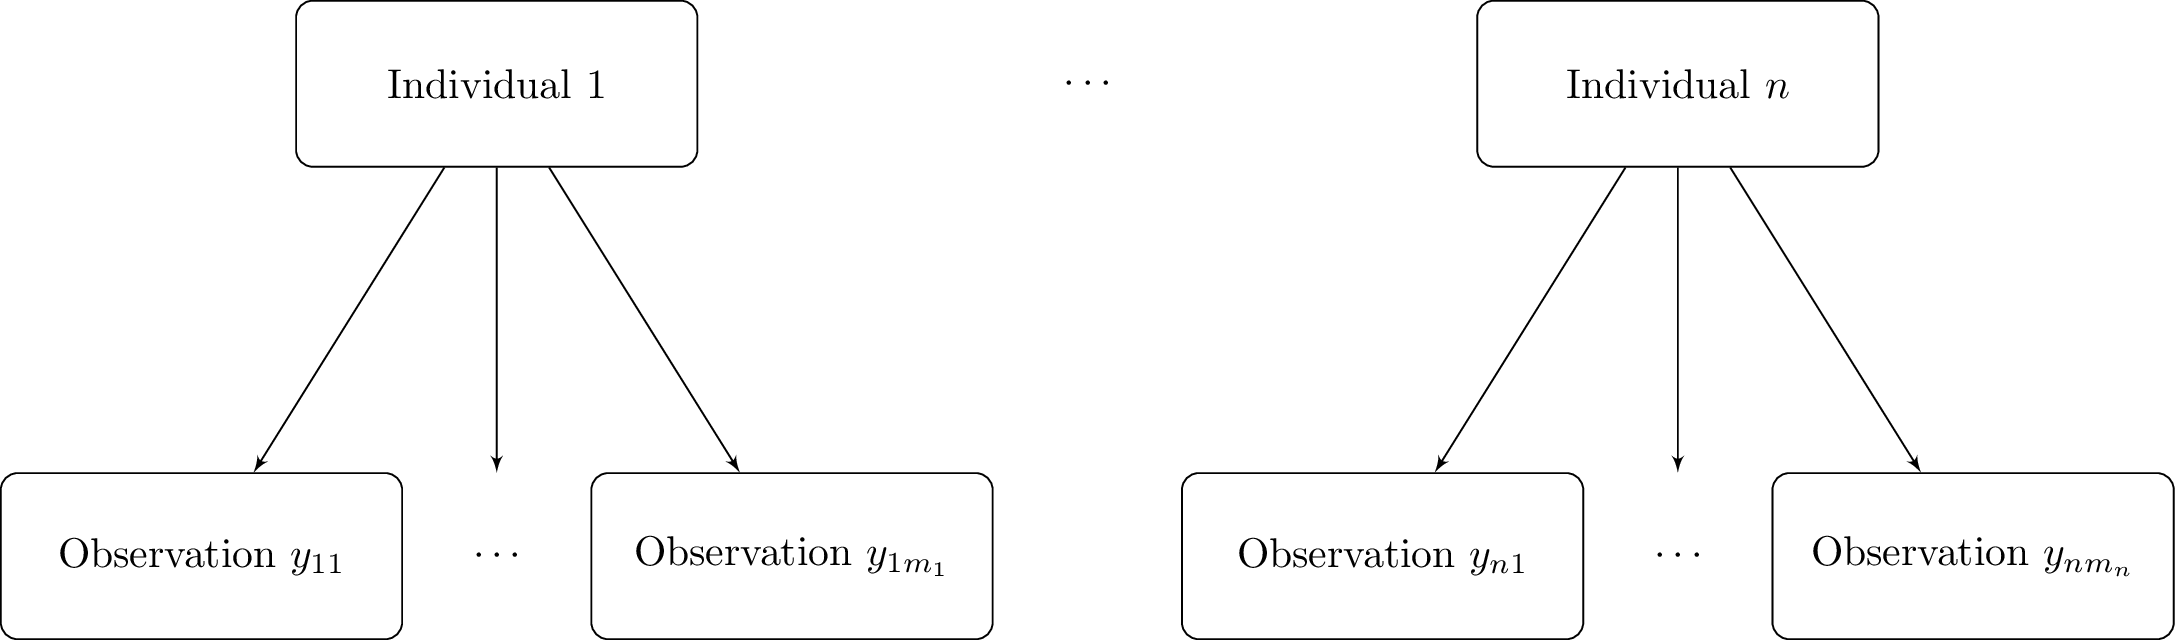
\includegraphics[width=0.95\linewidth]{figures/bayesian/hierarchical-structure} 

}

\caption{A simple example of group structure within data in which each individual \(i = 1, \ldots, n\) is associated to \(m_i\) observations \(y_{i1}, \ldots, y_{im_i}\).}\label{fig:hierarchical-structure}
\end{figure}

Group structure is a simple, binary way in which observations are related.
Figure \ref{fig:hierarchical-structure} illustrates a case in which each individual in a study is observed some number of times, and observations of the same individual are grouped together.
Observations from the same indivudal are more likely to be similar than observations of different individuals.
Groups can also be nested within other groups, as well as crossed with each other.

Consider three models for this data, each of which with a Gaussian likelihood:

\begin{enumerate}
\def\labelenumi{\arabic{enumi}.}
\tightlist
\item
  \textbf{Complete pooling}:
  In the complete pooling model, group structure is ignored and all observations are treated as IID
  \begin{align}
  y_{ij} \sim \mathcal{N}(\mu, \sigma), \\
  (\mu, \sigma) \sim p(\mu, \sigma).
  \end{align}
\item
  \textbf{No pooling}:
  Alternatively, the groups can be modelled entirely separately with group specific mean \(\mu_i\) and standard deviation \(\sigma_i\) parameters
  \begin{align}
  y_{ij} \sim \mathcal{N}(\mu_i, \sigma_i), \\
  (\mu_i, \sigma_i) \sim p(\mu_i, \sigma_i).
  \end{align}
\item
  \textbf{Partial pooling}:
  In this model, some amount of information is shared between the groups
  \begin{align}
  y_{ij} &\sim \mathcal{N}(\mu_i, \sigma), \\
  \mu_i &= \beta + u_i, \\
  \beta &\sim p(\beta), \\
  \mathbf{u} &\sim p(\mathbf{u}), \\
  \sigma &\sim p(\sigma),
  \end{align}
  where the vector \(\mathbf{u} = (u_1, \ldots, u_n)\).
  The parameter \(\beta\) applies to all groups, and each group is differentiated by a specific value of \(u_i\).
  When inference is performed for the partial pooling model, the extent to which information is shared between groups is learnt rather than fixed at the outset, as with the complete or no pooling models.
\end{enumerate}

Bayesian hierarchical or multilevel models allow control over whether and how information is shared across groups.
In a three-stage hierarchical model, the parameters are partitioned such that \(\boldsymbol{\mathbf{\phi}} = (\mathbf{x}, \boldsymbol{\mathbf{\theta}})\).
The model for data \(\mathbf{y}\) is then
\begin{align}
\mathbf{y} &\sim p(\mathbf{y} \, | \, \mathbf{x}, \boldsymbol{\mathbf{\theta}}), \\
\mathbf{x} &\sim p(\mathbf{x} \, | \, \boldsymbol{\mathbf{\theta}}), \\
\boldsymbol{\mathbf{\theta}} &\sim p(\boldsymbol{\mathbf{\theta}}),
\end{align}
with posterior distribution proportional to \(p(\mathbf{x}, \boldsymbol{\mathbf{\theta}} \, | \, \mathbf{y}) \propto p(\mathbf{y} \, | \, \mathbf{x}, \boldsymbol{\mathbf{\theta}}) p(\mathbf{x} \, | \, \boldsymbol{\mathbf{\theta}}) p(\boldsymbol{\mathbf{\theta}})\).
I refer to \(\mathbf{x} = (x_1, \ldots, x_n)\) as the latent field, and \(\boldsymbol{\mathbf{\theta}} = (\theta_1, \ldots, \theta_m)\) as the hyperparameters.

\hypertarget{generalised-linear-mixed-effects-model}{%
\subsection{Generalised linear mixed effects model}\label{generalised-linear-mixed-effects-model}}

Fixed effects refer to those elements of the latent field which are constant across groups.
Random effects refer to those elements of the latent field which vary across groups.
These terms have notoriously many different, and incompatible, definitions which can cause confusion \autocite{gelman2005analysis}.
I nonetheless find them useful to introduce here.

For concreteness, in the partial pooling model above, the latent field is \(\mathbf{x} = (\beta, u_1, \ldots, u_n)\).
The scalar \(\beta\) is a fixed effect which applies to all \(n\) groups.
The vector \(\mathbf{u}\) are random effects which alter the mean differently for each group.
The only hyperparameter is the standard deviation \(\theta = \sigma\).

Random effects can also be structured to share information between some groups more than others.
In spatio-temporal statistics, structured spatial and temporal random effects are often used to impose smoothness.
Spatial random effects are the subject of Chapter \ref{beyond-borders}.

Give equation for a generalised linear mixed model (GLMM) here.

\hypertarget{latent-gaussian-model}{%
\subsection{Latent Gaussian model}\label{latent-gaussian-model}}

Latent Gaussian models {[}LGMs; \textcite{rue2009approximate}{]} are a class of three-stage Bayesian hierarchical models in which the middle layer is Gaussian.
To be more precise, in an LGM, the likelihood is given by
\begin{align*}
y_i &\sim p(y_i \, | \, \eta_i, \boldsymbol{\mathbf{\theta}}_1), \quad i = 1, \ldots, n, \\
\mu_i &= \mathbb{E}(y_i \, | \, \eta_i) = g(\eta_i), \\
\eta_i &= \beta_0 + \sum_{l = 1}^{p} \beta_j z_{ji} + \sum_{k = 1}^{r} u_k(w_{ki}).
\end{align*}
Each response has conditional mean \(\mu_i\) with inverse link function \(g: \mathbb{R} \to \mathbb{R}\) such that \(\mu_i = g(\eta_i)\).
The likelihood has a product structure given by \(p(\mathbf{y} \, | \, \boldsymbol{\mathbf{\eta}}, \boldsymbol{\mathbf{\theta}}_1) = \prod_{i = 1}^n p(y_i \, | \, \eta_i, \boldsymbol{\mathbf{\theta}}_1)\), where \(\boldsymbol{\mathbf{\eta}} = (\eta_1, \ldots, \eta_n)\).
The vector \(\boldsymbol{\mathbf{\theta}}_1 \in \mathbb{R}^{s_1}\), with \(s_1\) assumed small, are additional parameters of the likelihood.
The structured additive predictor \(\eta_i\) may include an intercept \(\beta_0\), fixed effects \(\beta_j\) of the covariates \(z_{ji}\), and random effects \(u_k(\cdot)\) of the covariates \(w_{ki}\).
The parameters \(\beta_0\), \(\{\beta_j\}\), \(\{u_k(\cdot)\}\) are each assigned Gaussian prior distributions, and can be collected into a vector \(\mathbf{x} \in \mathbb{R}^N\) such that \(\mathbf{x} \sim \mathcal{N}(\mathbf{0}, \mathbf{Q}(\boldsymbol{\mathbf{\theta}}_2)^{-1})\) where \(\boldsymbol{\mathbf{\theta}}_2 \in \mathbb{R}^{s_2}\) are further hyperparameters, again with \(s_2\) assumed small.
Let \(\boldsymbol{\mathbf{\theta}} = (\boldsymbol{\mathbf{\theta}}_1, \boldsymbol{\mathbf{\theta}}_2) \in \mathbb{R}^m\) with \(m = s_1 + s_2\) be all hyperparameters, with prior distribution \(p(\boldsymbol{\mathbf{\theta}})\).

\hypertarget{extended-latent-gaussian-model}{%
\subsection{Extended latent Gaussian model}\label{extended-latent-gaussian-model}}

Extended latent Gaussian models {[}ELGMs; \textcite{stringer2022fast}{]} facilitate modelling of data with greater non-linearities than an LGM.
In an ELGM, the structured additive predictor is redefined as \(\boldsymbol{\mathbf{\eta}} = (\eta_1, \ldots \eta_{N_n})\), where \(N_n \in \mathbb{N}\) is a function of \(n\), and it is possible that \(N_n \neq n\).
Each mean response \(\mu_i\) now depends on some subset \(\mathcal{J}_i \subseteq [N_n]\) of indices of \(\boldsymbol{\mathbf{\eta}}\), with \(\cup_{i = 1}^n \mathcal{J}_i = [N_n]\) and \(1 \leq |\mathcal{J}_i| \leq N_n\), where \([N_n] = \{1, \ldots, N_n\}\).
The inverse link function \(g(\cdot)\) is redefined for each observation to be a possibly many-to-one mapping \(g_i: \mathbb{R}^{|\mathcal{J}_i|} \to \mathbb{R}\), such that \(\mu_i = g_i(\boldsymbol{\mathbf{\eta}}_{\mathcal{J}_i})\).
Put together, ELGMs are of the form
\begin{align*}
y_i &\sim p(y_i \, | \, \boldsymbol{\mathbf{\eta}}_{\mathcal{J}_i}, \boldsymbol{\mathbf{\theta}}_1), \quad i = 1, \ldots, n, \\
\mu_i &= \mathbb{E}(y_i \, | \, \boldsymbol{\mathbf{\eta}}_{\mathcal{J}_i}) = g_i(\boldsymbol{\mathbf{\eta}}_{\mathcal{J}_i}), \\
\eta_j &= \beta_0 + \sum_{l = 1}^{p} \beta_j z_{ji} + \sum_{k = 1}^{r} u_k(w_{ki}), \quad j = 1, \ldots, N_n,
\end{align*}
with latent field and hyperparameter prior distributions as in the LGM case.

The ELGM class is well suited to small-area estimation of HIV indicators, and so used throughout the thesis.
While it can be transformed to an LGM using the Poisson-multinomial transformation \autocite{baker1994multinomial} the multinomial logistic regression model used in Chapter \ref{multi-agyw} is naturally written as an ELGM where each observation depends on the set of structured additive predictors corresponding to the set of multinomial observations.
In Chapter \ref{naomi-aghq}, the Naomi small-area estimation model used to produce estimates of HIV indicators is shown to have the features of an ELGM.

\hypertarget{model-comparison}{%
\section{Model comparison}\label{model-comparison}}

Should this section be here?
Talk about: BF, AIC, BIC, WAIC, LOO, LOO-CV, connections, things used later in the thesis.

\hypertarget{survey}{%
\section{Survey methods}\label{survey}}

Large national household surveys provide the highest quality population-level information about HIV indicators in SSA.
Demographic and Health Surveys (DHS) are funded by the United States Agency for International Development (USAID) and run every three to five years in most countries.
Population-based HIV Impact Assessment (PHIA) surveys are funded by PEPFAR and run every four to five years in high HIV burden countries.

\hypertarget{survey-notation-and-key-terms}{%
\subsection{Survey notation and key terms}\label{survey-notation-and-key-terms}}

Consider a population of individuals \(i = 1, \ldots, N\) with outcomes of interest \(y_i\).
A census is a type of survey where all individuals are selected.
Supposing responses from all individuals were recorded, then any population means can be calculated directly.
For example, if \(G_i = G(y_i)\) then the population mean of \(G\) is
\begin{equation}
\bar G = \frac{1}{N} \sum_{i = 1}^N G(y_i).
\end{equation}

In practice, it is usually too expensive to run a census.
Instead, only a subset of the individuals are sampled.
Furthermore, only a subset of those sampled have their outcome recorded, due to nonresponse or otherwise.
Let \(S_i\) be an indicator for whether or not individual \(i\) is sampled, and \(R_i\) be an indicator for whether or not \(y_i\) is recorded.
If \(S_i = 0\) then \(R_i = 0\).
If \(S_i = 1\) then individual \(i\) may not respond such that \(R_i = 0\).
The population mean may be estimated directly based on the recorded subset of the population by
\begin{equation}
\bar G_R = \frac{\sum_{i = 1}^N R_i G(y_i)}{\sum_{i = 1}^N R_i}, \label{eq:direct}
\end{equation}
where \(m_R = \sum_{i = 1}^N R_i\) is the recorded sample size.

A probability sample refers to the case when individuals are selected to be included in the survey at random.
In a non-probability sample, inclusion or exclusion from the survey is deterministic.
A simple random sample (SRS) is a probability sample where the sampling probability for each individual is equal, so that \(P(S_i = 1) = 1 / N\).
The survey design is called complex when the sampling probabilities for each individual vary, such that \(P(S_i = 1) = \pi_i\) with \(\sum_{i = 1}^N \pi_i = 1\) and \(\pi_i > 0\).

Complex survey designs can offer both greater practicality and statistical efficiency than a SRS.
However, particular care is required in analysing data collected using complex survey designs.
Under a complex design, not accounting for unequal sampling probabilities will result in bias.
That said, even for a SRS, nonresponse can cause analogous bias.

\hypertarget{survey-design}{%
\subsection{Survey design}\label{survey-design}}

The DHS \autocite{measure2012sampling} employs a two-stage sampling procedure.
In the first stage, ennumeration areas (EAs) from a recently conducted census are typically used as the primary sampling unit (PSU).
The EAs are then stratified by region, as well as urban-rural.
After appropriate sample sizes are determined, EAs sampled with probability proportional to size (PPS) measured
In the second stage, the secondary sampling units (SSUs) are households.
All households in the selected EAs are listed, before being sampled systematically.
Finally, each selected household is visited, and all adults are interviewed.

The probability an individual is sampled is equal to the probability their household is sampled.
The first-stage sampling probability of the \(j\)th cluster in stratum \(h\) given by
\begin{equation}
\pi_{1hj} = n_h \times \frac{N_{hj}}{\sum_j N_{hj}},
\end{equation}
where \(N_{hj}\) is the number of households and \(n_h\) be the number of clusters selected in stratum \(h\).
The second-stage sampling probability each household within the \(i\)th cluster in stratum \(h\) is
\begin{equation}
\pi_{1hj} = \frac{n_{hj}}{N_{hj}},
\end{equation}
where \(n_{hj}\) is the number of households selected in cluster \(j\) and stratum \(h\).
That is, each household in the cluster has equal selection probability.
The overall selection probability of each household in cluster \(j\) of stratum \(h\) is \(\pi_{hi} = \pi_{1hj} \times \pi_{2hj}\).

\hypertarget{survey-analysis}{%
\subsection{Survey analysis}\label{survey-analysis}}

Suppose a complex survey is run with sampling probabilities \(\pi_i\).
The standard method for taking into account that some individuals are more likely to be included in the survey than others is to overweight the responses of those unlikely to be included, and underweight the responses of those likely to be included.
This can be achieved using design weights \(\delta_i = 1 / \pi_i\), which can be thought of as the number of individuals in the population represented by the \(i\)th sampled individual.
Let \(P(R_i = 1 \, | \, S_i = 1) = \upsilon_i\) be the probability of response for sampled individual \(i\).
The problem of nonresponse can be treated in the same way using nonresponse weights \(\gamma_i = 1 / \upsilon_i\), which analogously can be thought of as the number of sampled individuals represented by the \(i\)th recorded individual.
Multiplying the design and nonresponse weights gives survey weights \(\omega_i = \delta_i \times \gamma_i\).

A weighted estimate \autocite{hajek1971discussion} of the population mean using the survey weights \(\omega_i\) is given by
\begin{equation}
\bar G_\omega = \frac{\sum_{i = 1}^N \omega_j R_i G(y_i)}{\sum_{i = 1}^N \omega_i R_i}. \label{eq:hajek}
\end{equation}
Decomposing the additive error of this estimate provides useful intuition as to the potential benefits of survey weighting.
Following \textcite{meng2018statistical} then under SRS
\begin{align}
\bar G_\omega - \bar G &= \frac{\mathbb{E}(\omega_i R_i G_i)}{\mathbb{E}(\omega_i R_i)} - \mathbb{E}(G_i) = \frac{\mathbb{C}(\omega_i R_i G_i)}{\mathbb{E}(\omega_i R_i)} \\ 
&= \rho_{R_\omega, G} \times \sqrt{\frac{N - m_{R_\omega}}{m_{R_\omega}}} \times \sigma_G,
\end{align}
where \(R_\omega = \omega R\).
The data defect correlation (DDC) \(\rho_{R_\omega, G}\) measures the correlation between the weighted recording mechanism and given function of the outcome of interest.
To minimise the DDC then \(G \perp \!\!\! \perp R_\omega\).
The data scarcity \(\sigma_{R_\omega} = \sqrt{(N - m_{R_\omega})/m_{R_\omega}}\) measures the effective proportion of the population who have been recorded.
The problem difficultly \(\sigma_G\) measures the intrinsic difficulty of the estimation problem, and is independent of the sampling or analysis method.

For simplicity, let \(G(y_i) = y_i\) and each \(y_i \in \{0, 1\}\).
We weight then model following \textcite{chen2014use}.
While this approach acknowledges the survey design, it has some important limitations.
We ignore clustering structure.
All of this isn't great and that someone should figure this out \autocite{gelman2007struggles}.

\hypertarget{beyond-borders}{%
\chapter{Models for spatial structure}\label{beyond-borders}}

\adjustmtc
\markboth{Models for spatial structure}{}

This chapter presents an investigation of spatial random effects specifications.
My investigation was motivated by a fundamental question encountered during model construction.
Namely, should the model be augmented to capture a conjectured feature of the data?
The results are presented in \textcite{howes2023beyond}.
Code for the analysis in this chapter is available from \href{https://github.com/athowes/beyond-borders}{\texttt{https://github.com/athowes/beyond-borders}}.

\hypertarget{background-1}{%
\section{Background}\label{background-1}}

\hypertarget{models-based-on-adjacency}{%
\section{Models based on adjacency}\label{models-based-on-adjacency}}

\hypertarget{the-besag-model}{%
\subsection{The Besag model}\label{the-besag-model}}

Spatial structure can be encoded using a symmetric relation between areas.
Let \(i \sim j\) if the areas \(A_i\) and \(A_j\) are adjacent or neighbouring.
Adjacency is often defined by a shared border, though other choices are possible \autocite{paciorek2013spatial}.
The Besag model \autocite{besag1991bayesian} is an improper conditional auto-regressive (ICAR) model where the full conditional distribution of the \(i\)th spatial random effect is given by
\begin{equation}
    u_i \, | \, \mathbf{u}_{-i} \sim \mathcal{N} \left(\frac{1}{n_{\delta i}} \sum_{j: j \sim i} u_j, \frac{1}{n_{\delta i}\tau_u}\right), \label{eq:besag}
\end{equation}
where \(\delta i\) is the set of neighbours of \(A_i\) with cardinality \(n_{\delta i} = |\delta i|\) and \(\mathbf{u}_{-i}\) is the vector of spatial random effects with the \(i\)th entry removed.
The conditional mean of the random effect \(u_i\) is the average of its neighbours \(\{u_j\}_{j \sim i}\) and the precision \(n_{\delta i}\tau_u\) is proportional to the number of neighbours \(n_{\delta i}\).
By Brook's lemma \autocite{rue2005gaussian} the set of full conditionals of the Besag model are equivalent to the Gaussian Markov random field (GMRF) given by
\begin{equation}
    \mathbf{u} \sim \mathcal{N}(\mathbf{0}, \tau_u^{-1} \mathbf{R}^{-}), \label{eq:gmrf}
\end{equation}
where \(\mathbf{R}^{-}\) is the generalised inverse of the rank-deficient structure matrix \(\mathbf{R}\), so-called because it defines the structure of the precision matrix, with entries
\begin{equation}
    R_{ij} =
    \begin{cases}
        n_{\delta i}, & i = j \\
        -1, & i \sim j \\
        0, & \text{otherwise.}
    \end{cases}
\end{equation}
The Markov property arises due to the conditional independence structure \(p(u_i \, | \, \mathbf{u}_{-i}) = p(u_i \, | \, \mathbf{u}_{\delta i})\) whereby each area only depends on its neighbours.
This is reflected in the sparsity of \(\mathbf{R}\) such that \(u_i \perp u_j \, | \, \mathbf{u}_{-ij}\) if and only if \(R_{ij} = 0\).
The structure matrix \(\mathbf{R}\) may also be expressed as the Laplacian of the adjacency graph \(\mathcal{G} = (\mathcal{V}, \mathcal{E})\) with vertices \(v \in \mathcal{V}\) corresponding to each area and edges \(e \in \mathcal{E}\) between vertices \(i\) and \(j\) when \(i \sim j\).

Rewriting Equation \eqref{eq:gmrf}, the probability density function of \(\mathbf{u}\) is
\begin{equation}
    p(\mathbf{u})
    \propto \exp \left( -\frac{\tau_u}{2} \mathbf{u}^\top \mathbf{R} \mathbf{u} \right)
    \propto \exp \left( -\frac{\tau_u}{2} \sum_{i \sim j} (u_i - u_j)^2 \right). \label{eq:pdfu}
\end{equation}
This density is a function of the pairwise differences \(u_i - u_j\) and so is invariant to the addition of a constant \(c\) to each entry \(p(\mathbf{u}) = p(\mathbf{u} + c\mathbf{1})\), leading to an improper uniform distribution on the average of the \(u_i\).
If \(\mathcal{G}\) is connected, in that by traversing the edges, any vertex can be reached from any other vertex, then there is only one impropriety in the model and \(\text{rank}(\mathbf{R}) = n - 1\), while if \(\mathcal{G}\) is disconnected, and composed of \(n_c \geq 2\) connected components with index sets \(I_1, \ldots, I_{n_c}\), then the corresponding structure matrix \(\mathbf{R}\) has rank \(n - n_c\) and the density is invariant to the addition of a constant to each of the connected components \(p(\mathbf{u}_{I}) = p(\mathbf{u}_{I} + c\mathbf{1})\) where \(I = I_1, \ldots, I_{n_c}\).

\hypertarget{best-practises-for-the-besag-model}{%
\subsection{Best practises for the Besag model}\label{best-practises-for-the-besag-model}}

\textcite{freni2018note} recommended three best practices:

\begin{enumerate}
\def\labelenumi{\arabic{enumi}.}
\tightlist
\item
  The structure matrix \(\mathbf{R}\) should be rescaled to have generalised variance, defined by the geometric mean of the diagonal elements of its generalised inverse
  \begin{equation}
   \sigma^2_{\text{GV}}(\mathbf{R}) = \prod_{i = 1}^n (\mathbf{R}^-_{ii})^{1/n} = \exp \left( \frac{1}{n} \sum_{i = 1}^n \log (\mathbf{R}^-_{ii}) \right),
  \end{equation}
  equal to one, by replacing \(\mathbf{R}\) with \(\mathbf{R}^\star = \mathbf{R} / \sigma^2_{\text{GV}}(\mathbf{R})\).
  As the diagonal elements \(R^-_{ii}\) correspond to marginal variances, the generalised variance gives a measure of the average marginal variance.
  However, this measure, introduced by \textcite{sorbye2014scaling}, ignores off-diagonal entries and more broadly any measure of typical variance could be used.
  Scaling mitigates the influence of the adjacency graph on the variance of \(\mathbf{u}\).
  Allowing the variance to be controlled by \(\tau_u\) alone is important as it allows for consistent, interpretable prior selection.
\end{enumerate}

When the adjacency graph is disconnected it is not appropriate to scale the structure matrix \(\mathbf{R}\) uniformly since for a given precision \(\tau_u\), local smoothing operates on each connected component independently.
As such, each connected component should be scaled independently to have generalised variance one giving \(\mathbf{R}^\star_I = \mathbf{R}_I / \sigma^2_{\text{GV}}(\mathbf{R}_I)\) where \(\mathbf{R}_I\) is the sub-matrix of the structure matrix corresponding to index set \(I\).

\begin{enumerate}
\def\labelenumi{\arabic{enumi}.}
\setcounter{enumi}{1}
\tightlist
\item
  When one of the connected components is a single area, known either as a singleton or an island, the probability density \(\exp \left( -\frac{\tau_u}{2} \sum_{i \sim j} (u_i - u_j)^2 \right)\) has no dependence on \(u_i\).
  This is equivalent to using an improper prior \(p(u_i) \propto 1\) and can be avoided by setting each singleton to have independent Gaussian noise \(p(u_i) \sim \mathcal{N}(0, 1)\).
\item
  To avoid confounding of the spatial random effects with the intercept, it is recommended to place a sum-to-zero constraint on each non-singleton connected component.
  In other words, for each \(|I| > 1\) that \(\sum_{i \in I} u_i = 0\).
\end{enumerate}

\hypertarget{the-reparameterised-besag-york-molliuxe9-model}{%
\subsection{The reparameterised Besag-York-Mollié model}\label{the-reparameterised-besag-york-molliuxe9-model}}

Often, as well as spatial structure, there exists IID over-dispersion in the residuals and it is inappropriate to use purely spatially structured random effects in the model.
The Besag-York-Mollié (BYM) model of \textcite{besag1991bayesian} accounts for this in a natural way by decomposing the spatial random effect \(\mathbf{u} = \mathbf{v} + \mathbf{w}\) into a sum of an unstructured IID component \(\mathbf{v}\) and a spatially structured Besag component \(\mathbf{w}\), each of which with their own respective precision parameters \(\tau_v\) and \(\tau_w\).
The resulting distribution is
\begin{equation}
    \mathbf{u} \sim \mathcal{N}(0, \tau_v^{-1} \mathbf{I} + \tau_w^{-1} \mathbf{R}^{-}) \label{eq:bym}.
\end{equation}
Including both \(\mathbf{v}\) and \(\mathbf{w}\) is intended to enable the model to learn the relative extent of the unstructured and structured components via \(\tau_v\) and \(\tau_w\).
However, in this specification scaling of the Besag precision matrix \(\mathbf{Q}\) is not taken into account despite this issue being particularly pertinent when dealing with multiple sources of noise.
In particular, placing a joint prior \((\tau_v, \tau_w) \sim p(\tau_v, \tau_w)\) which doesn't privilege either component is more easily accomplished if \(\mathbf{Q}\) and \(\mathbf{I}\) have the same scale.
Additionally, supposing we have a prior belief that the over-dispersion is primarily IID and \(\mathbf{v}\) accounts for the majority of the dispersion, then it is not immediately obvious how to represent this belief using \(p(\tau_v, \tau_w)\), without inadvertently altering the prior about the overall variation.
This highlights identifiability issues of the parameters \((\tau_v, \tau_w)\) resulting from them not being orthogonal.
Building on the models of \textcite{leroux2000estimation} and \textcite{dean2001detecting} which tackle this identifiability problem, but do not scale the spatially structured noise, \textcite{simpson2017penalising} propose a reparameterisation \((\tau_v, \tau_w) \mapsto (\tau_u, \phi)\) of the BYM model known as the BYM2 model and given by
\begin{align}
\mathbf{u} = \frac{1}{\tau_u} \left( \sqrt{1- \phi} \, \mathbf{v} + \sqrt{\phi} \, \mathbf{w}^\star \right), \label{eq:bym2}
\end{align}
where \(\tau_u\) is the marginal precision of \(\mathbf{u}\), \(\phi \in [0, 1]\) gives the proportion of the marginal variance explained by each component, and \(\mathbf{w}^\star\) is a scaled version of \(\mathbf{w}\) with precision matrix given by the scaled structure matrix \(\mathbf{R}^\star\).
When \(\phi = 0\) the random effects are IID, and when \(\phi = 1\) the random effects follow the Besag model.
To borrow an analogy \autocite{rue2020comment} the parameterisation \((\tau_v, \tau_w)\) is like having one hot water and one cold water tap, whereas the parameterisation \((\tau_u, \phi)\) is like a mixer tap where the amount of water and its temperature can be adjusted separately.

\hypertarget{concerns-about-the-besag-models-representation-of-space}{%
\subsection{Concerns about the Besag model's representation of space}\label{concerns-about-the-besag-models-representation-of-space}}

The Besag model was originally proposed for use in image analysis, where areas correspond to pixels arranged in a regular lattice structure.
Since then, it has seen wider use, including in situations, like small-area estimation of HIV, where the spatial structure is less regular.
As such, I have a number of concerns about the model's applicability to this broader setting.
This discussion is closely linked to the modifiable areal unit problem \autocite{openshow1979million}, whereby statistical conclusions change as a result of seemingly arbitrary changes in data aggregation, as well as the challenge of ecological inference and the ecological fallacy \autocite{wakefield2010aggregation}.



\begin{figure}

{\centering 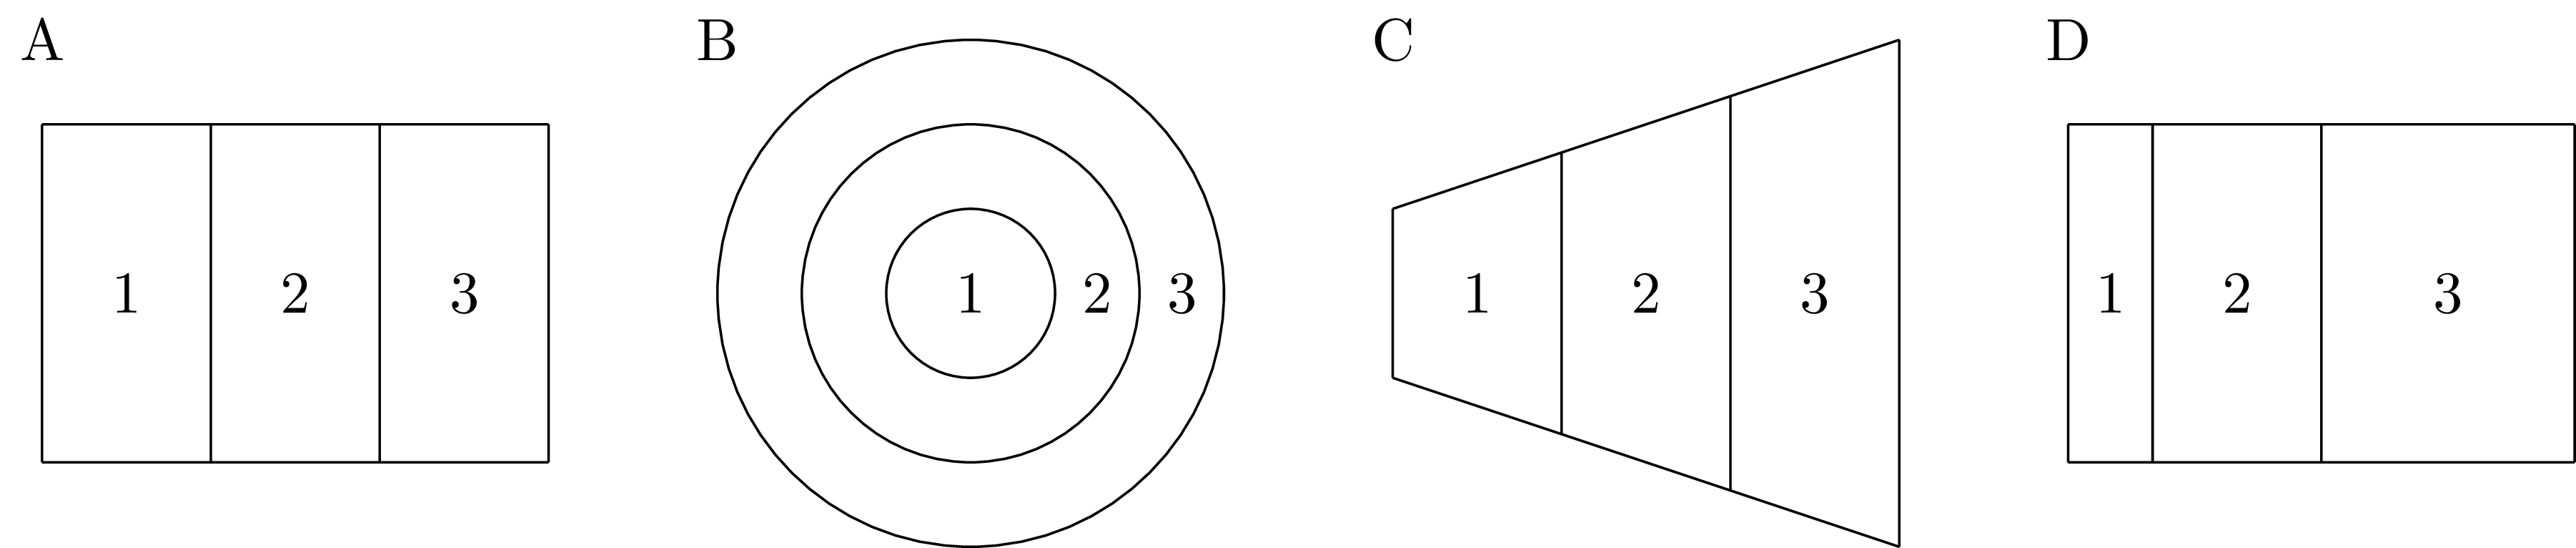
\includegraphics[width=0.95\linewidth]{resources/beyond-borders/temp/depends/maup1} 

}

\caption{Figure caption.}\label{fig:maup1}
\end{figure}



\begin{figure}

{\centering 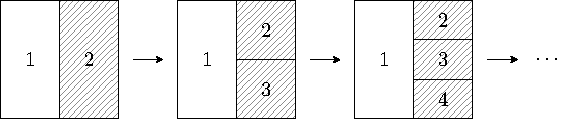
\includegraphics[width=0.95\linewidth]{resources/beyond-borders/temp/depends/maup2} 

}

\caption{Figure caption.}\label{fig:maup2}
\end{figure}



\begin{figure}

{\centering 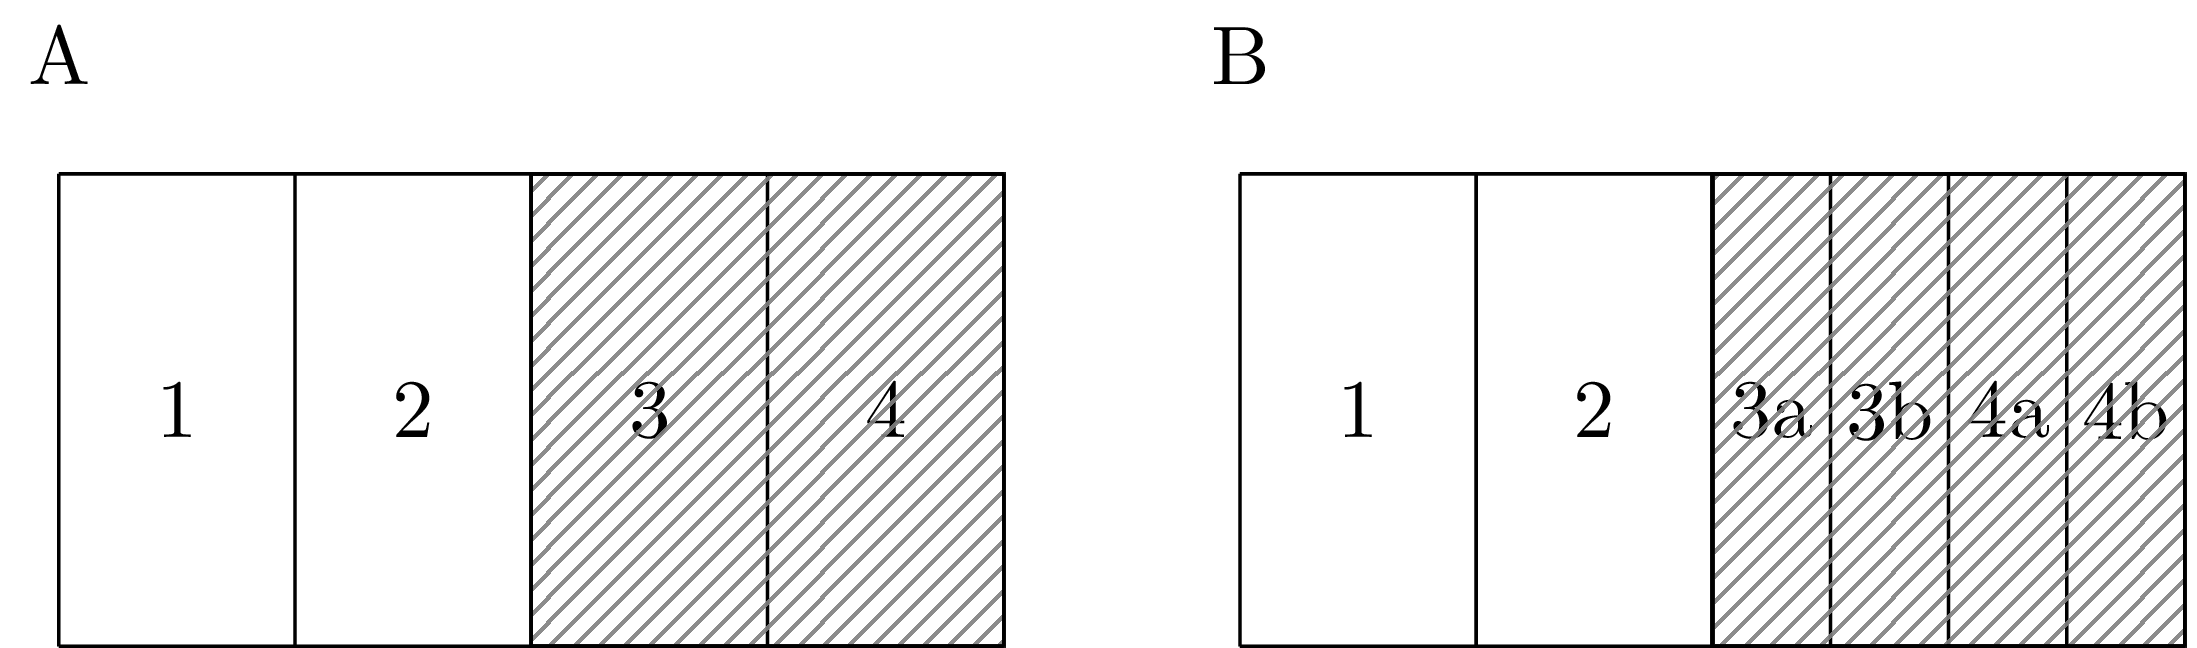
\includegraphics[width=0.95\linewidth]{resources/beyond-borders/temp/depends/maup3} 

}

\caption{Figure caption.}\label{fig:maup3}
\end{figure}

\hypertarget{adjacency-compression}{%
\subsubsection{Adjacency compression}\label{adjacency-compression}}

Summarising a geometry by an adjacency graph represents a loss of information.
Many geometries share the same adjacency graph, and are as such isomorphic identical under the Besag model (Figure).
This is not in itself a problem, but does prompt consideration as to whether the class of geometries with the same adjacency graph is sufficiently similar to merit identical models.\footnote{The regularity of realistic geometries may help to constrain each class to be more similar than it strictly has to be. In other words, although pathological geometries can be constructed, they are implausible in statistical practise and so not of great concern to us here.}
Intuitively, the more regular the spatial structure, the less information is lost in compression to an adjacency graph.
In image analysis, very little spatial information is lost in compression of a lattice structure to an adjacency graph.
On the other hand, the regions of a country, determined by political and geographic forces, tend to display greater irregularity.
The appropriateness of adjacency compression therefore varies by the type of geometry common to the application setting.

\hypertarget{mean-structure}{%
\subsubsection{Mean structure}\label{mean-structure}}

In the Besag model is all adjacent areas count equally.
This assumption is unsatisfying: for most geometries, we expect different amounts of correlation between neighbours.
Figure illustrates a number of heuristic features for neighbour importance, including length of shared border, and the proximity of centers of mass.

\hypertarget{variance-structure}{%
\subsubsection{Variance structure}\label{variance-structure}}

In Equation \eqref{eq:besag} the precision of \(u_i\) is proportional to its number of neighbours \(n_{\delta i}\).
It follow that as \(n_{\delta i} \to \infty\) then \(\text{Var}(u_i) \to 0\).
This is illustrated by Figure where the area on the right is repeatedly divided such that its number of neighbours increases.
This property is a consequence of averaging the conditional mean over a greater number of areas, which, in certain situations, can correspond to a greater amount of information.
However, if the amount of information in the shaded area remains fixed, it is inappropriate that \(\text{Var}(u_1)\) should tend to zero as a result of drawing additional, arbitrary, boundaries.
In the image analysis setting this modelling assumption is reasonable: each pixel represents a fixed amount of information and a higher pixel density represents a greater amount of information.
On the other hand, in public health and epidemiology, drawing boundaries to create additional areas is not expected to correspond to a greater amount of information.

Suppose we fit a Besag model upon identical data using each of the two geometries in Figure.
If the spatial variation is relatively smooth, dividing the shaded areas into two will result in a lower estimated variance \(\sigma^2_u\) in geometry (ii) as compared with geometry (i) because there will appear to be less variation between neighbouring areas.
This problem does not only apply locally: since the effect of \(\sigma^2_u\) applies everywhere, the smoothing will change even in unaltered parts of the study region.

\hypertarget{models-using-kernels}{%
\section{Models using kernels}\label{models-using-kernels}}

\hypertarget{simulation-study}{%
\section{Simulation study}\label{simulation-study}}

\hypertarget{hiv-prevalence-study}{%
\section{HIV prevalence study}\label{hiv-prevalence-study}}

\hypertarget{discussion}{%
\section{Discussion}\label{discussion}}

\textcite{follestad2003modelling}

\hypertarget{multi-agyw}{%
\chapter{A model for risk group proportions}\label{multi-agyw}}

\adjustmtc
\markboth{A model for risk group proportions}{}

This chapter describes an application of Bayesian spatio-temporal statistics to small-area estimation of HIV risk group proportions.
This work was conducted in collaboration with colleagues from the MRC Centre for Global Infectious Disease Analysis and UNAIDS.
I developed the statistical model, building upon an earlier version of the analysis conducted by Dr.~Kathryn Risher.
The model and results for 13 countries are presented in \textcite{howes2023spatio}, and implemented in a spreadsheet tool (\href{https://hivtools.unaids.org/pse/}{\texttt{https://hivtools.unaids.org/pse/}}) for use in national HIV response planning.
The tool is being updated by inclusion of more countries to the analysis, and extension of the methodology, including to additional risk groups.
Code for the analysis in this chapter is available from \href{https://github.com/athowes/multi-agyw}{\texttt{https://github.com/athowes/multi-agyw}}.

\hypertarget{background-2}{%
\section{Background}\label{background-2}}

In SSA, adolescent girls and young women (AGYW) aged 15-29 are at increased risk of HIV infection.
Though AGYW are only 28\% of the population, they comprise 44\% of new infections \autocite{unaids2021update}.
HIV incidence for AGYW is 2.4 times higher than for similarly aged (15-29) males.
The social and biological reasons for this disparity include structural vulnerabilities and power imbalances, age patterns of sexual mixing, a younger age at first sex, and increased susceptibility to HIV infection.
On this basis, AGYW have been identified as a priority population for HIV prevention services.
Significant investments, such as the DREAMS partnership \autocite{saul2018dreams} and by the the Global Fund \autocite{global2018measurement}, have been made to support prevention programming.

The Global AIDS Strategy 2021-2026 \autocite{unaids2021global} was adopted by the United Nations (UN) General Assembly in June 2021, and ``outlines the strategic priorities and actions to be implemented by global, regional, country and community partners to get on-track to ending AIDS''.
It proposed stratifying HIV prevention packages to AGYW based on two factors

\begin{enumerate}
\def\labelenumi{\arabic{enumi}.}
\tightlist
\item
  local population-level HIV incidence, and
\item
  individual-level sexual risk behaviour.
\end{enumerate}

Risk of acquiring HIV depends on both factors.
As such, prioritisation of prevention services is more efficient if both factors are taken into account.
I illustrate this stylistically in Figure \ref{fig:risk-grid}.
The strategy encourages programmes to define targets for the proportion of AGYW to be reached with a range of interventions.
Implementation of the strategy by national HIV programmes and stakeholders requires data on the population size and HIV incidence in each risk group by location.



\begin{figure}

{\centering 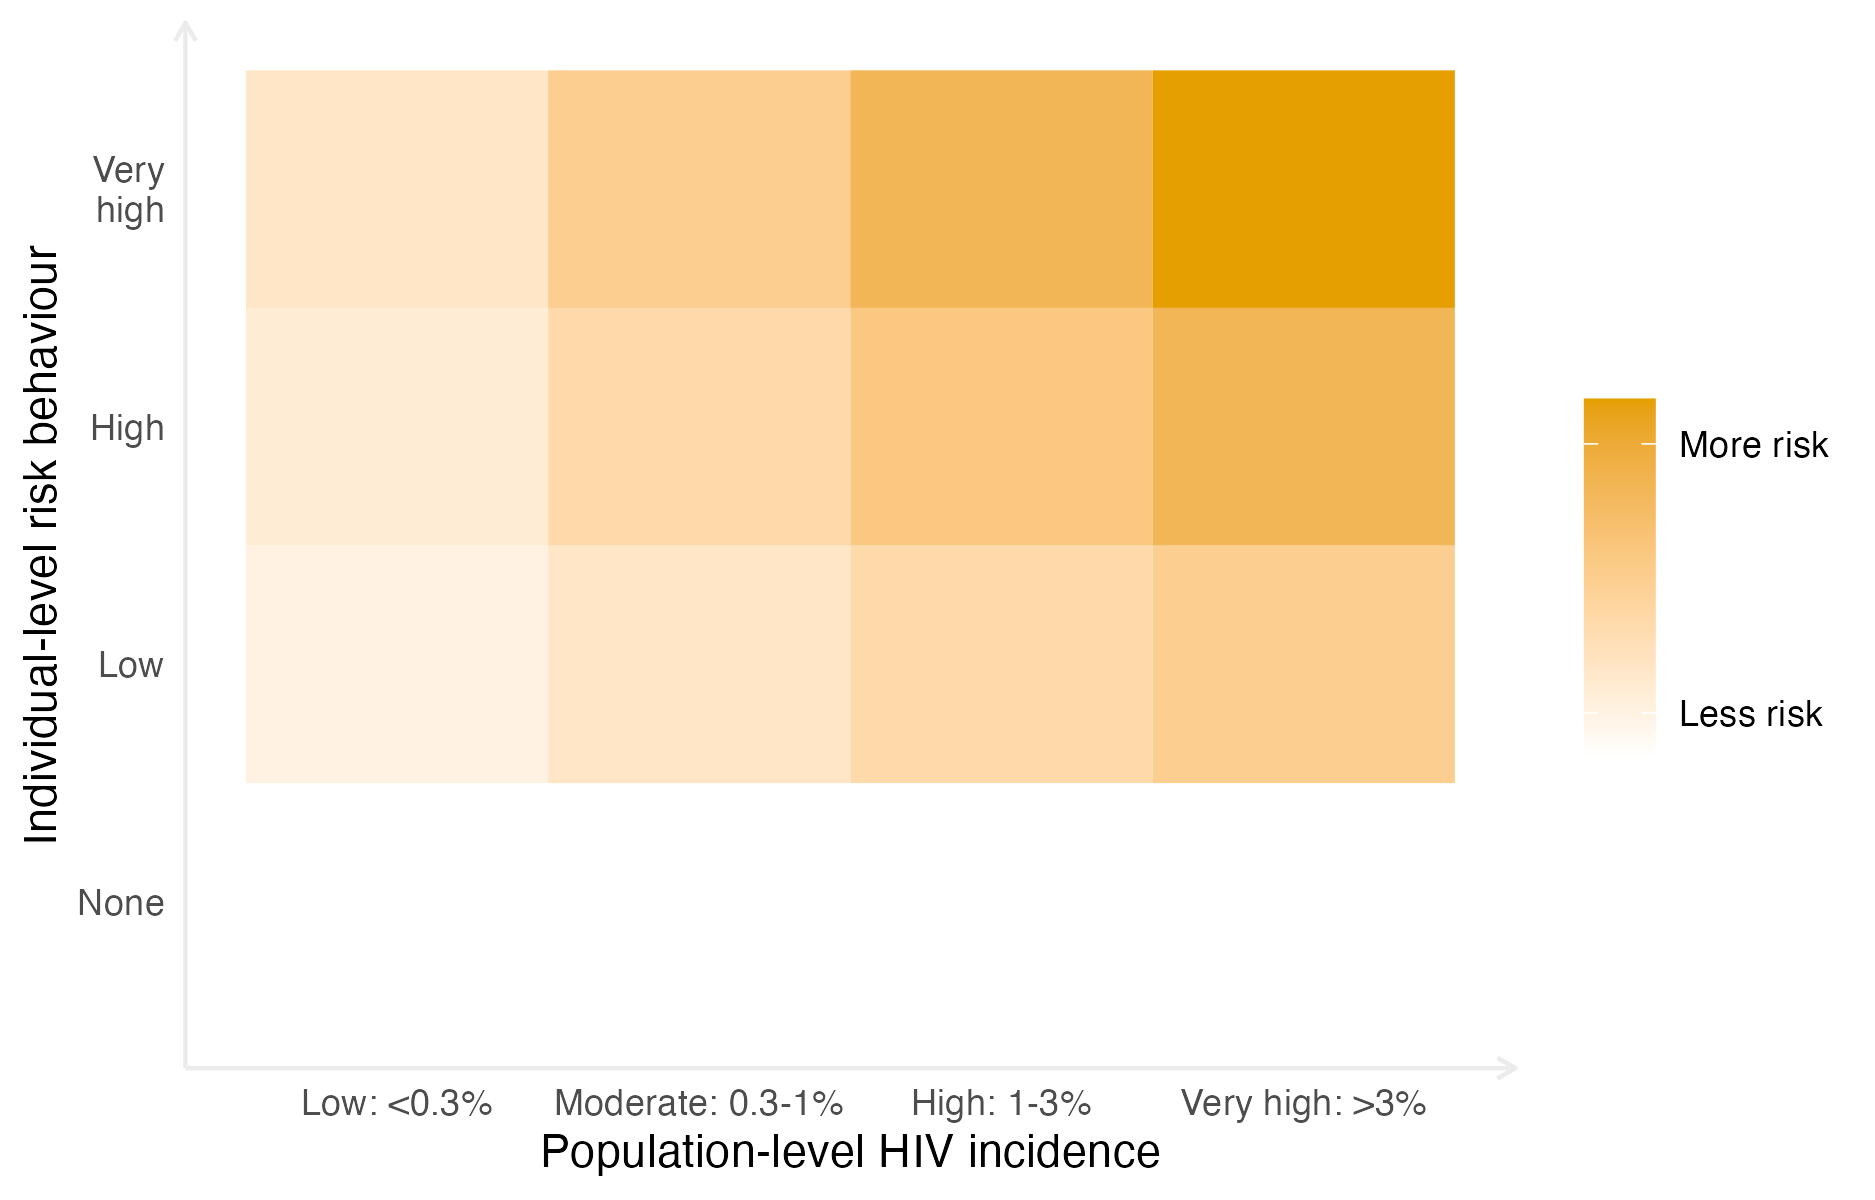
\includegraphics[width=0.95\linewidth]{figures/multi-agyw/risk-grid} 

}

\caption{Risk of acquiring HIV is depends on both individual-level risk behaviour and population-level HIV incidence. I assume that with no individual-level risk behaviour, there is no risk of acquiring HIV, independent of the population-level HIV incidence. The risk scale is intended to be illustrative, rather than interpreted quantitatively.}\label{fig:risk-grid}
\end{figure}

\hypertarget{data-1}{%
\section{Data}\label{data-1}}

\hypertarget{behavioural-data-from-household-surveys}{%
\subsection{Behavioural data from household surveys}\label{behavioural-data-from-household-surveys}}

\begin{longtable}[]{@{}
  >{\raggedright\arraybackslash}p{(\columnwidth - 4\tabcolsep) * \real{0.2778}}
  >{\raggedright\arraybackslash}p{(\columnwidth - 4\tabcolsep) * \real{0.3056}}
  >{\raggedright\arraybackslash}p{(\columnwidth - 4\tabcolsep) * \real{0.4167}}@{}}
\caption{\label{tab:risk-groups} HIV risk groups and HIV incidence rate ratios relative to AGYW with one cohabiting sexual partner.
The incidence rate ratio for women with non-regular or multiple sexual partner(s) was derived from analysis of longitudinal data by \textcite{slaymaker2020croi}.
Among FSW, the incidence rate ratio (25.0, 13.0, 9.0, 6.0, 3.0) depended on the level of HIV incidence among the general population (\textless0.1\%, 0.1-0.3\%, 0.3-1.0\%, 1.0-3.0\%, \textgreater3.0\%), such that higher local HIV incidence in the general population corresponded to a lower incidence rate ratio for FSW.
Estimates of HIV incidence rate ratios for FSW were derived by UNAIDS based on patterns of relative HIV prevalence among FSW compared to general population prevalence.}\tabularnewline
\toprule\noalign{}
\begin{minipage}[b]{\linewidth}\raggedright
Risk group
\end{minipage} & \begin{minipage}[b]{\linewidth}\raggedright
Description
\end{minipage} & \begin{minipage}[b]{\linewidth}\raggedright
Incidence rate ratio
\end{minipage} \\
\midrule\noalign{}
\endfirsthead
\toprule\noalign{}
\begin{minipage}[b]{\linewidth}\raggedright
Risk group
\end{minipage} & \begin{minipage}[b]{\linewidth}\raggedright
Description
\end{minipage} & \begin{minipage}[b]{\linewidth}\raggedright
Incidence rate ratio
\end{minipage} \\
\midrule\noalign{}
\endhead
\bottomrule\noalign{}
\endlastfoot
None & Not sexually active & 0.0 \\
Low & One cohabiting sexual partner & 1.0 (baseline) \\
High & Non-regular or multiple partner(s) & 1.72 \\
Very High & Reporting transactional sex (later adjusted to correspond to FSW) & 3.0-25.0 (varied depending on local HIV incidence) \\
\end{longtable}

I used household survey data from 13 countries identified by the the Global Fund \autocite{global2018measurement} as priority countries for implementation of AGYW HIV prevention.
These countries were Botswana, Cameroon, Kenya, Lesotho, Malawi, Mozambique, Namibia, South Africa, Eswatini, Tanzania, Uganda, Zambia and Zimbabwe.
Surveys conducted in these countries between 1999 and 2018 were included in which both women were interviewed about their sexual behaviour, and sufficient geographic information was available to locate survey clusters to health districts.
There were 46 suitable surveys (Figure \ref{fig:available-surveys}), with a total sample size of 274,970 women aged 15-29 years.
Of the respondents, 103,063 were aged 15-19 years, 92,173 were aged 20-24 years, and 79,734 were aged 25-29 years.
The median number of surveys per country was four, ranging from one in Botswana and South Africa to six in Uganda.



\begin{figure}

{\centering 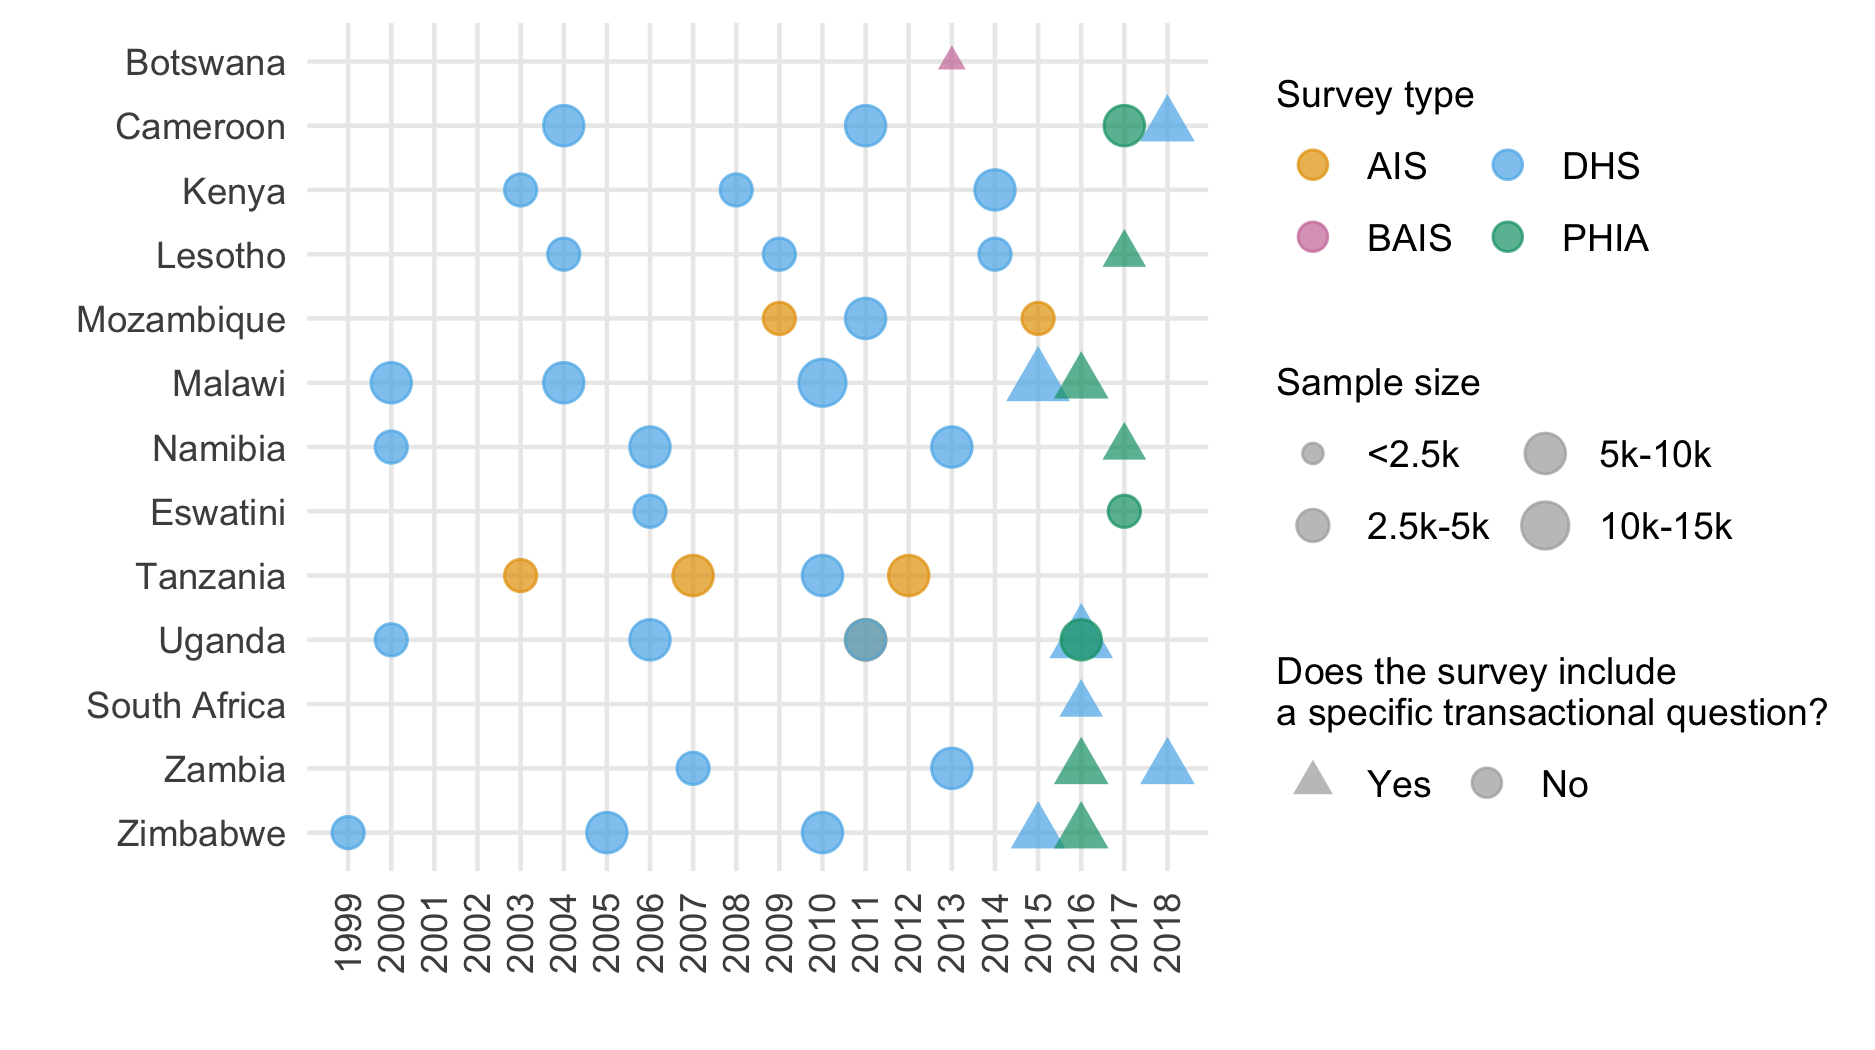
\includegraphics[width=0.95\linewidth]{resources/multi-agyw/20230627-144735-3da88508/depends/available-surveys} 

}

\caption{Surveys conducted 1999-2018 that were used in the analysis by year, survey type, sample size, and whether the survey included a specific question about transactional sex. Survey type included AIDS Indicator Surveys (AIS), Demographic and Health Surveys (DHS), the Botswana AIDS Impact Survey 2013 (BAIS), and Population-based HIV Impact Assessment (PHIA) surveys.}\label{fig:available-surveys}
\end{figure}

For each survey, I classified respondents into one of four behavioural risk groups \(k = 1, 2, 3, 4\) according to reported sexual risk behaviour in the past 12 months (Figure \ref{fig:category-flowchart}).
In increasing order of HIV acquisition risk, these risk groups were:

\begin{itemize}
\tightlist
\item
  \(k = 1\): Not sexually active
\item
  \(k = 2\): One cohabiting sexual partner
\item
  \(k = 3\): Non-regular or multiple sexual partner(s), and
\item
  \(k = 4\): Reporting transactional sex.
\end{itemize}

The HIV incidence rate ratio \(\text{RR}_k\) was assumed to vary by risk group (Table \ref{tab:risk-groups}), with the one cohabiting partner risk group as baseline.

Exact survey questions varied slightly across survey types and between survey phases.
Questions captured information about whether the respondent had been sexually active in the past twelve months, and if so with how many partners.
For their three most recent partners, respondents were also asked about the type of partnership.
Possible partnership types included spouse, cohabiting partner, partner not cohabiting with respondent, friend, sex worker, sex work client, and other.
Full survey questions used are in Appendix \ref{survey-questions}.
In the case of inconsistent responses, women were categorised according to the highest risk group they fell into, ensuring that the categories were mutually exclusive.

Some surveys included a specific question asking if the respondent had received or given money or gifts for sex in the past twelve months.
In these surveys, 2.64\% of women reported transactional sex.
In surveys without such a question, women almost never (0.01\%) answered that one of their three most recent partners was a sex work client.
This incomparability made it inappropriate to include surveys without a specific transactional sex question when estimating the proportion of the population who engaged in transactional sex.
Of the total 46 surveys included in the analysis, 12 had a specific transactional sex question, with a total sample size of 62,853 (28,753 aged 15-19 years, 26,324 aged 20-24 years, and 7,776 aged 25-29 years).
The sample size for women aged 25-29 is smaller because there were 6 DHS surveys which excluded women 25-29 from the transactional sex survey question.



\begin{figure}

{\centering 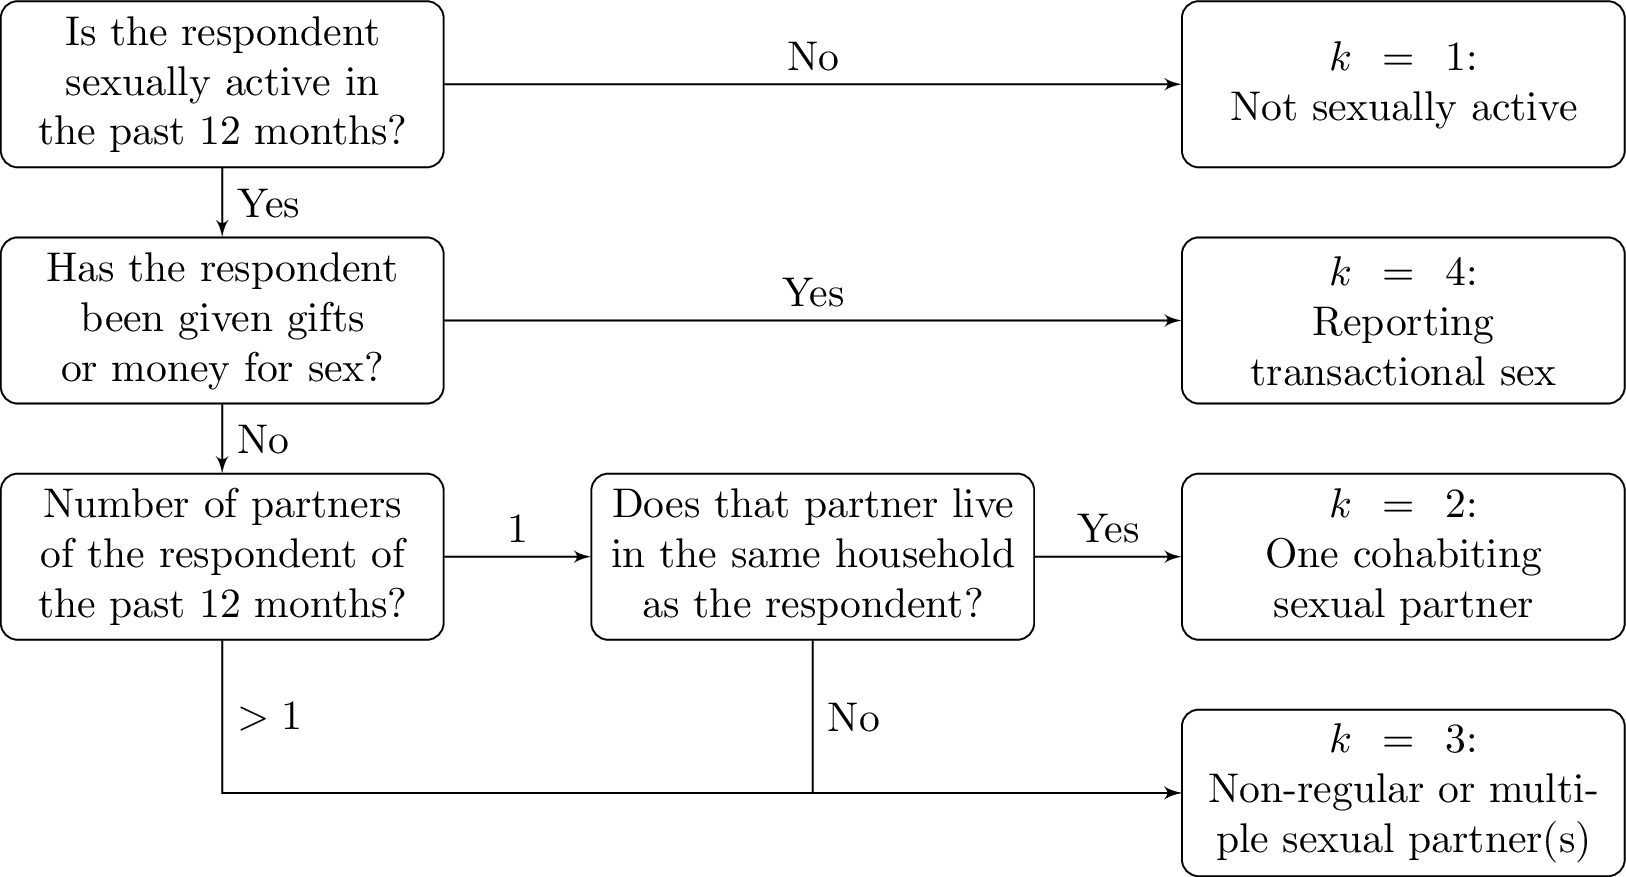
\includegraphics[width=0.95\linewidth]{figures/multi-agyw/category-flowchart} 

}

\caption{Flowchart giving classification of survey respondents to HIV risk groups.}\label{fig:category-flowchart}
\end{figure}

\hypertarget{other-data}{%
\subsection{Other data}\label{other-data}}

In addition to the household survey behavioural data, I used estimates of population, PLHIV and new HIV infections stratified by district and age group from HIV estimates published by UNAIDS that were developed using the Naomi model \autocite{eaton2021naomi}.
I used the most recent 2022 estimates for all countries, apart from Mozambique where, due to data accuracy concerns, I used the 2021 estimates (in which the Cabo Delgado province is excluded due to disruption by conflict).
I used administrative area hierarchy and geographic boundaries corresponding to those used for health service planning by countries.
Exceptions were Cameroon and Kenya, where I conducted analyses one level higher at the department and county levels, respectively.

\hypertarget{model-for-risk-group-proportions}{%
\section{Model for risk group proportions}\label{model-for-risk-group-proportions}}

Owing to the incomparability in estimating the \(k = 4\) risk gorup across surveys, I took a two-stage modelling approach to estimate the four risk group proportions.
Denote being in either the third or fourth risk group as \(k = 3^{+}\).
First, using all the surveys, I used a spatio-temporal multinomial logistic regression model to estimate the proportion of AGYW in the risk groups \(k \in \{1, 2, 3^{+}\}\).
This model is described in Section \ref{st-multinomial}.
Then, using only those surveys with a specific transactional sex question, I fit a spatial logistic regression model to estimate the proportion of those in the \(k = 3^{+}\) risk group that were in the \(k = 3\) and \(k = 4\) risk groups respectively.
This model is described in Section \ref{s-logistic}.

\hypertarget{st-multinomial}{%
\subsection{Spatio-temporal multinomial logistic regression}\label{st-multinomial}}

Let \(i \in \{1, \ldots, n\}\) denote districts partitioning the 13 studied AGYW priority countries \(c[i] \in \{1, \ldots, 13\}\).
Consider the years 1999-2018 denoted as \(t \in \{1, \ldots, T\}\), and age groups \(a \in \{\text{15-19}, \text{20-24}, \text{25-29}\}\).
Let \(p_{itak} > 0\) with \(\sum_{k = 1}^{3^{+}} p_{itak} = 1\), be the probabilities of membership of risk group \(k\).

\hypertarget{multinomial-logistic-regression}{%
\subsubsection{Multinomial logistic regression}\label{multinomial-logistic-regression}}

A standard multinomial logistic regression model \autocite[e.g.][]{gelman2013bayesian} is specified by
\begin{align}
    \mathbf{y}_{ita} &= (y_{ita1}, \ldots, y_{ita3^{+}})^\top \sim \text{Multinomial}(m_{ita}; \, p_{ita1}, \ldots, p_{ita3^{+}}), \label{eq:mlr1} \\
    \log \left( \frac{p_{itak}}{p_{ita1}} \right) &= \eta_{itak}, \quad k = 2, 3^{+}, \label{eq:mlr2}
\end{align}
where the number in risk group \(k\) is \(y_{itak}\), the fixed sample size is \(m_{ita} = \sum_{k = 1}^{3^{+}} y_{itak}\), and \(k = 1\) is chosen as the baseline category.
This model is not an LGM because each observation \(y_{itak}\) for \(k \in \{1, 2, 3^{+}\}\) depends on multiple structured additive predictors \(\{\eta_{itak}, k = 1, 2, 3^{+}\}\).

The model, defined over 940 districts, 20 years, 3 age groups, and 3 risk groups, is too large for MCMC to be tractable in reasonable time.
To recast this model as an LGM, I used the multinomial-Poisson transformation (detailed in Section \ref{mp-transformation}).
This modification allowed inference to be performed using the INLA \autocite{rue2009approximate} algorithm via the \texttt{R-INLA} package \autocite{martins2013bayesian}.
Inferences from INLA in the LGM setting are accurate and substantially faster than MCMC.

\hypertarget{mp-transformation}{%
\subsubsection{The multinomial-Poisson transformation}\label{mp-transformation}}

The multinomial-Poisson transformation \autocite{baker1994multinomial} reframes a given multinomial logistic regression model, like that described in Equations \eqref{eq:mlr1} and \eqref{eq:mlr2}, as an equivalent Poisson log-linear model.
The equivalent model is of the form
\begin{align}
    y_{itak} &\sim \text{Poisson}(\kappa_{itak}), \label{eq:poisson1} \\
    \log(\kappa_{itak}) &= \eta_{itak}. \label{eq:poisson2}
\end{align}
The basis of the transformation is that conditional on their sum Poisson counts are jointly multinomially distributed \autocite{mccullagh1989generalized} as follows
\begin{equation}
    \mathbf{y}_{ita} \, | \, m_{ita} \sim \text{Multinomial} \left( m_{ita}; \frac{\kappa_{ita1}}{\kappa_{ita}}, \ldots, \frac{\kappa_{ita3^{+}}}{\kappa_{ita}} \right), \label{eq:multi}
\end{equation}
where \(\kappa_{ita} = \sum_{k = 1}^{3^{+}} \kappa_{itak}\).
The probabilities \(p_{itak}\) may then be obtained using the softmax function
\begin{equation}
    p_{itak} = \frac{\exp(\eta_{itak})}{\sum_{k = 1}^{3^{+}} \exp(\eta_{itak})} = \frac{\kappa_{itak}}{\sum_{k = 1}^{3^{+}} \kappa_{itak}} = \frac{\kappa_{itak}}{\kappa_{ita}}.
\end{equation}
Under the equivalent model, in Equation \eqref{eq:poisson1} the sample sizes \(m_{ita}\) are treated as random rather than fixed such that
\begin{equation}
m_{ita} = \sum_k y_{itak} \sim \text{Poisson} \left( \sum_k \kappa_{itak} \right) = \text{Poisson} \left( \kappa_{ita} \right). \label{eq:mpoisson}
\end{equation}
Using Equations \eqref{eq:multi} for \(p(\mathbf{y}_{ita} \, | \, m_{ita})\) and Equation \eqref{eq:mpoisson} for \(p(m_{ita})\), the joint distribution is given by
\begin{align}
p(\mathbf{y}_{ita}, m_{ita}) &= \exp(-\kappa_{ita}) \frac{(\kappa_{ita})^{m_{ita}}}{m_{ita}!} \times \frac{m_{ita}!}{\prod_k y_{itak}!} \prod_k \left( \frac{\kappa_{itak}}{\kappa_{ita}} \right)^{y_{itak}} \\
&= \prod_k \left( \frac{\exp(-\kappa_{itak}) \left( \kappa_{itak} \right)^{y_{itak}}}{y_{itak}!} \right) \\
&= \prod_k \text{Poisson} \left( y_{itak} \, | \, \kappa_{itak} \right). \label{eq:prodpoisson}
\end{align}
As expected, Equation \eqref{eq:prodpoisson} corresponds to the product of independent Poisson likelihoods defined in Equation \eqref{eq:poisson1}.
This exercise demonstrates that the Poisson log-linear model contains within it a multinomial likelihood, with a Poission prior on the sample size.

For this model to be equivalent to a multinomial logistic regression model, the normalisation constants \(m_{ita}\) must be recovered exactly.
That is to say, their posterior distributions should be as close as possible to a Dirac delta distribution with value zero everywhere but the known value of the sample size.
To ensure that this is the case, observation-specific random effects \(\theta_{ita}\) can be included in the equation for the linear predictor.
Multiplying each of \(\{\kappa_{itak}\}_{k = 1}^{3^+}\) by \(\exp(\theta_{ita})\) has no effect on the category probabilities, but does provide the necessary flexibility for \(\kappa_{ita}\) to recover \(m_{ita}\) exactly.
Although in theory an improper prior distribution \(\theta_{ita} \propto 1\) should be used, I found that in practice, by keeping \(\eta_{ita}\) otherwise small using appropriate constraints, so that arbitrarily large values of \(\theta_{ita}\) are not required, it is sufficient (and practically preferable for inference) to instead use a vague prior distribution.

\hypertarget{model-specifications}{%
\subsubsection{Model specifications}\label{model-specifications}}

\begin{longtable}[]{@{}
  >{\raggedright\arraybackslash}p{(\columnwidth - 10\tabcolsep) * \real{0.0202}}
  >{\raggedright\arraybackslash}p{(\columnwidth - 10\tabcolsep) * \real{0.1818}}
  >{\raggedright\arraybackslash}p{(\columnwidth - 10\tabcolsep) * \real{0.2020}}
  >{\raggedright\arraybackslash}p{(\columnwidth - 10\tabcolsep) * \real{0.1818}}
  >{\raggedright\arraybackslash}p{(\columnwidth - 10\tabcolsep) * \real{0.1919}}
  >{\raggedright\arraybackslash}p{(\columnwidth - 10\tabcolsep) * \real{0.2222}}@{}}
\caption{\label{tab:multinomial-models} Four multinomial regression models were considered. Observation random effects \(\theta_{ita}\), included in all models, are omitted from this table.}\tabularnewline
\toprule\noalign{}
\begin{minipage}[b]{\linewidth}\raggedright
\end{minipage} & \begin{minipage}[b]{\linewidth}\raggedright
Category \(\beta_k\)
\end{minipage} & \begin{minipage}[b]{\linewidth}\raggedright
Country \(\zeta_{ck}\)
\end{minipage} & \begin{minipage}[b]{\linewidth}\raggedright
Age \(\alpha_{ack}\)
\end{minipage} & \begin{minipage}[b]{\linewidth}\raggedright
Spatial \(\phi_{ik}\)
\end{minipage} & \begin{minipage}[b]{\linewidth}\raggedright
Temporal \(\gamma_{tk}\)
\end{minipage} \\
\midrule\noalign{}
\endfirsthead
\toprule\noalign{}
\begin{minipage}[b]{\linewidth}\raggedright
\end{minipage} & \begin{minipage}[b]{\linewidth}\raggedright
Category \(\beta_k\)
\end{minipage} & \begin{minipage}[b]{\linewidth}\raggedright
Country \(\zeta_{ck}\)
\end{minipage} & \begin{minipage}[b]{\linewidth}\raggedright
Age \(\alpha_{ack}\)
\end{minipage} & \begin{minipage}[b]{\linewidth}\raggedright
Spatial \(\phi_{ik}\)
\end{minipage} & \begin{minipage}[b]{\linewidth}\raggedright
Temporal \(\gamma_{tk}\)
\end{minipage} \\
\midrule\noalign{}
\endhead
\bottomrule\noalign{}
\endlastfoot
M1 & IID & IID & IID & IID & IID \\
M2 & IID & IID & IID & Besag & IID \\
M3 & IID & IID & IID & IID & AR1 \\
M4 & IID & IID & IID & Besag & AR1 \\
\end{longtable}

I considered four models (Table \ref{tab:multinomial-models}) for \(\eta_{ita}\) in the equivalent Poisson log-linear model of the form
\begin{equation}
\eta_{ita} = \theta_{ita} + \beta_k + \zeta_{c[i]k} + \alpha_{ac[i]k} + u_{ik} + \gamma_{tk}.
\end{equation}
Observation random effects \(\theta_{ita} \sim \mathcal{N}(0, 1000^2)\) with a vague prior distribution were included in all models to ensure the multinomial-Poisson transformation was valid.
To capture country-specific proportion estimates for each category, I included category random effects \(\beta_k \sim \mathcal{N}(0, \tau_\beta^{-1})\) and country-category random effects \(\zeta_{ck} \sim \mathcal{N}(0, \tau_\zeta^{-1})\).
Heterogeneity in risk group proportions by age was allowed by including age-country-category random effects \(\alpha_{ack} \sim \mathcal{N}(0, \tau_\alpha^{-1})\).
I considered several specifications for the space-cateogry \(u_{ik}\) and time-cateogry effects \(\gamma_{tk}\), described in Sections \ref{spatial-re} and \ref{temporal-re}.

Use of the multinomial-Poisson transformation required all random effects to include interaction with category \(k\), because any random effects which did not include interaction with category would give no change in category probabilities.
The only exception were the observation random effects, which were included as a device to ensure the transformation is valid, rather than to model the data.

\hypertarget{spatial-re}{%
\paragraph{Spatial random effects}\label{spatial-re}}

For the space-category random effects \(u_{ik}\) I considered two specifications:

\begin{enumerate}
\def\labelenumi{\arabic{enumi}.}
\tightlist
\item
  Independent and identically distributed (IID) \(u_{ik} \sim \mathcal{N}(0, \tau_u^{-1})\),
\item
  The Besag improper conditional autoregressive (ICAR) model \autocite{besag1991bayesian} grouped by category
  \[
  \mathbf{u} = (u_{11}, \ldots, u_{n1}, \ldots, u_{1{3^{+}}}, \ldots u_{n3^{+}})^\top \sim \mathcal{N}(\mathbf{0}, (\tau_u \mathbf{R}^\star_u)^{-}).
  \]
  The scaled structure matrix \(\mathbf{R}^\star_u = \mathbf{R}^\star_b \otimes \mathbf{I}\) is given by the Kronecker product of the scaled Besag structure matrix \(\mathbf{R}^\star_b\) and the identity matrix \(\mathbf{I}\), and \({-}\) denotes the generalised matrix inverse.
  I followed best practices for the Besag model as described in Chapter \ref{beyond-borders}.
  To implement the Kronecker product I used the \texttt{group} option in \texttt{R-INLA} {[}Section 3.5.5; \textcite{gomez2020bayesian}{]} setting the random effect to be \texttt{f(area\_idx,\ model\ =\ "besag",\ group\ =\ cat\_idx,\ control.group\ =\ list(model\ =\ "iid"),\ ...)}.
  Though the Kronecker product is symmetric, performance is better in \texttt{R-INLA} when the more complicated effect is written as the first variable rather than the grouping variable.
\end{enumerate}

In preliminary testing I used the BYM2 model \autocite{simpson2017penalising} in place of the Besag.
I found that the proportion parameter posteriors tended to be highly peaked at the value one.
For simplicity and to avoid numerical issues, by using Besag random effects I effectively decided to fix this proportion to one.

\hypertarget{temporal-re}{%
\paragraph{Temporal random effects}\label{temporal-re}}

For the time-category random effects \(\gamma_{tk}\) I considered two specifications:

\begin{enumerate}
\def\labelenumi{\arabic{enumi}.}
\tightlist
\item
  IID \(\gamma_{tk} \sim \mathcal{N}(0, \tau_\gamma^{-1})\),
\item
  First order autoregressive (AR1) grouped by category
  \[
  \boldsymbol{\mathbf{\gamma}} = (\gamma_{11}, \ldots, \gamma_{13^{+}}, \ldots, \gamma_{T1}, \ldots, \gamma_{T3^{+}})^\top \sim \mathcal{N}(\mathbf{0}, (\tau_\gamma \mathbf{R}^\star_\gamma)^{-}).
  \]
  The scaled structure matrix \(\mathbf{R}^\star_\gamma = \mathbf{R}^\star_r \otimes \mathbf{I}\) is given by the Kronecker product of a scaled AR1 structure matrix \(\mathbf{R}^\star_r\) and the identity matrix \(\mathbf{I}\).
  The AR1 structure matrix \(\mathbf{R}_r\) is obtained by precision matrix of the random effects \(\mathbf{r} = (r_1, \ldots, r_T)^\top\) specified by
  \begin{align}
  r_1 &\sim \left( 0, \frac{1}{1 - \rho^2} \right), \\
  r_t &= \rho r_{t - 1} + \epsilon_t, \quad t = 2, \ldots, T, 
  \end{align}
  where \(\epsilon_t \sim \mathcal{N}(0, 1)\) and \(|\rho| < 1\).
  As with the structured spatial random effects, I implemented this Kronecker product using the \texttt{group} option via \texttt{f(year\_idx,\ model\ =\ "ar1",\ group\ =\ cat\_idx,\ control.group\ =\ list(model\ =\ "iid"),\ ...)}.
  Again the more complicated variable was written first.
\end{enumerate}

\hypertarget{a-note-on-spatio-temporal-interaction-random-effects}{%
\paragraph{A note on spatio-temporal interaction random effects}\label{a-note-on-spatio-temporal-interaction-random-effects}}

I also considered including separable space-time-category random effects \(\delta_{itk}\) in the model, using the specification
\begin{equation}
    \boldsymbol{\mathbf{\delta}} = (\delta_{111}, \ldots, \delta_{nT3^{+}})^\top \sim \mathcal{N}(\mathbf{0}, (\tau_\delta \mathbf{R}^\star_\delta)^{-}),
\end{equation}
where \(\mathbf{R}^\star_\delta\) is a Kronecker product of the relevant space, time and category structure matrices.
These specifications were:

\begin{enumerate}
\def\labelenumi{\arabic{enumi}.}
\tightlist
\item
  IID spatial and IID temporal (Type I) \(\mathbf{R}^\star_\delta = \mathbf{I} \otimes \mathbf{I} \otimes \mathbf{I}\),
\item
  Besag spatial and IID temporal (Type II) \(\mathbf{R}^\star_\delta = \mathbf{R}^\star_b \otimes \mathbf{I} \otimes \mathbf{I}\),
\item
  IID spatial and AR1 temporal (Type III) \(\mathbf{R}^\star_\delta = \mathbf{I} \otimes \mathbf{R}^\star_a \otimes \mathbf{I}\),
\item
  Besag spatial and AR1 (Type IV) \(\mathbf{R}^\star_\delta = \mathbf{R}^\star_b \otimes \mathbf{R}^\star_a \otimes \mathbf{I}\),
\end{enumerate}

where the first, second and third elements of the Kronecker product represent space, time and category (always IID) structure matrices respectively.
The interaction type in brackets (e.g.~Type I) is given according to the \textcite{knorr2000bayesian} framework.

Though three-way Kronecker products are not directly supported in \texttt{R-INLA}, I implemented each specification using a combination of the \texttt{group} and \texttt{replicate} options {[}Section 6.5.2; \textcite{gomez2020bayesian}{]}.
For example, for the Type IV effects the random effects were specified by \texttt{f(area\_idx\_copy,\ model\ =\ "besag",\ group\ =\ year\_idx,\ replicate\ =\ cat\_idx,\ control.group\ =\ list(model\ =\ "ar1"))}.
I was able to run these models for single countries, keeping only years at which surveys occurred in those countries.
However, when fitting all countries jointly I found inclusion of the space-time-category random effects to be intractable, and as such decided not to include them in the model.

\hypertarget{prior-distributions}{%
\paragraph{Prior distributions}\label{prior-distributions}}

All random effect precision parameters \(\tau \in \{\tau_\beta, \tau_\zeta, \tau_\alpha, \tau_u, \tau_\gamma, \tau_\delta\}\) were given independent penalised complexity (PC) prior distributions \autocite{simpson2017penalising} with base model \(\sigma = 0\) given by
\begin{equation}
p(\tau) = 0.5 \nu \tau^{-3/2} \exp \left( - \nu \tau^{-1/2} \right)
\end{equation}
where \(\nu = - \ln(0.01) / 2.5\) such that \(\mathbb{P}(\sigma > 2.5) = 0.01\).
For the lag-one correlation parameter \(\rho\), I used the PC prior distribution, as derived by \textcite{sorbye2017penalised}, with base model \(\rho = 1\) and condition \(\mathbb{P}(\rho > 0 = 0.75)\).
I chose the base model \(\rho = 1\) corresponding to no change in behaviour over time, rather than the alternative \(\rho = 0\) corresponding to no correlation in behaviour over time, as I judged the former to be more plausible a priori.

\hypertarget{identifiability-constraints}{%
\subsubsection{Identifiability constraints}\label{identifiability-constraints}}

To facilitate interpretability of the posterior inferences, I applied sum-to-zero constraints (Table \ref{tab:constraints}) such that none of the category interaction random effects altered overall category probabilities.
In testing of the space-time-category random effects, I applied analogous sum-to-zero constraints to maintain roles of the space-category and time-category random effects.
In some cases it was not possible to implement all three sets of constraints for the three-way interactions in \texttt{R-INLA}.

\begin{longtable}[]{@{}
  >{\raggedright\arraybackslash}p{(\columnwidth - 2\tabcolsep) * \real{0.5600}}
  >{\raggedright\arraybackslash}p{(\columnwidth - 2\tabcolsep) * \real{0.4400}}@{}}
\caption{\label{tab:constraints} Applying sum-to-zero constraints to interaction effects ensures that the main effect is not interfered with.}\tabularnewline
\toprule\noalign{}
\begin{minipage}[b]{\linewidth}\raggedright
Random effects
\end{minipage} & \begin{minipage}[b]{\linewidth}\raggedright
Constraints
\end{minipage} \\
\midrule\noalign{}
\endfirsthead
\toprule\noalign{}
\begin{minipage}[b]{\linewidth}\raggedright
Random effects
\end{minipage} & \begin{minipage}[b]{\linewidth}\raggedright
Constraints
\end{minipage} \\
\midrule\noalign{}
\endhead
\bottomrule\noalign{}
\endlastfoot
Category & \(\sum_k \beta_k = 0\) \\
Country & \(\sum_c \zeta_{ck} = 0, \, \forall \, k\) \\
Age-country & \(\sum_a \alpha_{ack} = 0, \, \forall \, c, k\) \\
Spatial & \(\sum_i u_{ik} = 0, \, \forall \, k\) \\
Temporal & \(\sum_t \gamma_{tk} = 0, \, \forall \, k\) \\
Spatio-temporal & \(\sum_i \delta_{itk} = 0, \, \forall \, t, k; \sum_t \delta_{itk} = 0, \, \forall \, i, k; \sum_k \delta_{itk} = 0, \, \forall \, i, t\) \\
\end{longtable}

\hypertarget{survey-weighted-likelihood}{%
\subsubsection{Survey weighted likelihood}\label{survey-weighted-likelihood}}

I accounted for the survey design using a weighted pseudo-likelihood where the observed counts \(y\) are replaced by effective counts \(y^\star\), as described in Section \ref{survey}.
These counts may not be integers, and as such the Poisson likelihood given in Equation \eqref{eq:poisson1} is not appropriate.
Instead, I used a generalised Poisson pseudo-likelihood \(y^\star \sim \text{xPoisson}(\kappa)\) given by
\begin{equation}
    p(y^\star) = \frac{\kappa^{y^\star}}{\left \lfloor{y^\star!}\right \rfloor } \exp \left(- \kappa \right),
\end{equation}
to extend the Poisson distribution to non-integer weighted counts.
This working likelihood is implemented by \texttt{family\ =\ "xPoisson"} in \texttt{R-INLA}.

\hypertarget{model-selection}{%
\subsubsection{Model selection}\label{model-selection}}

I selected the model including Besag spatial random effects and IID temporal random effects based on the conditional predictive ordinate (CPO) criterion \autocite{pettit1990conditional}.
For comparison, I also computed the deviance information criterion (DIC) \autocite{spiegelhalter2002bayesian} and widely applicable information criterion (WAIC) \autocite{watanabe2013widely}.
Each of these criterion can be calculated in \texttt{R-INLA} without requiring model refitting.
The results are presented in Figure \ref{fig:model-comparison}.



\begin{figure}

{\centering 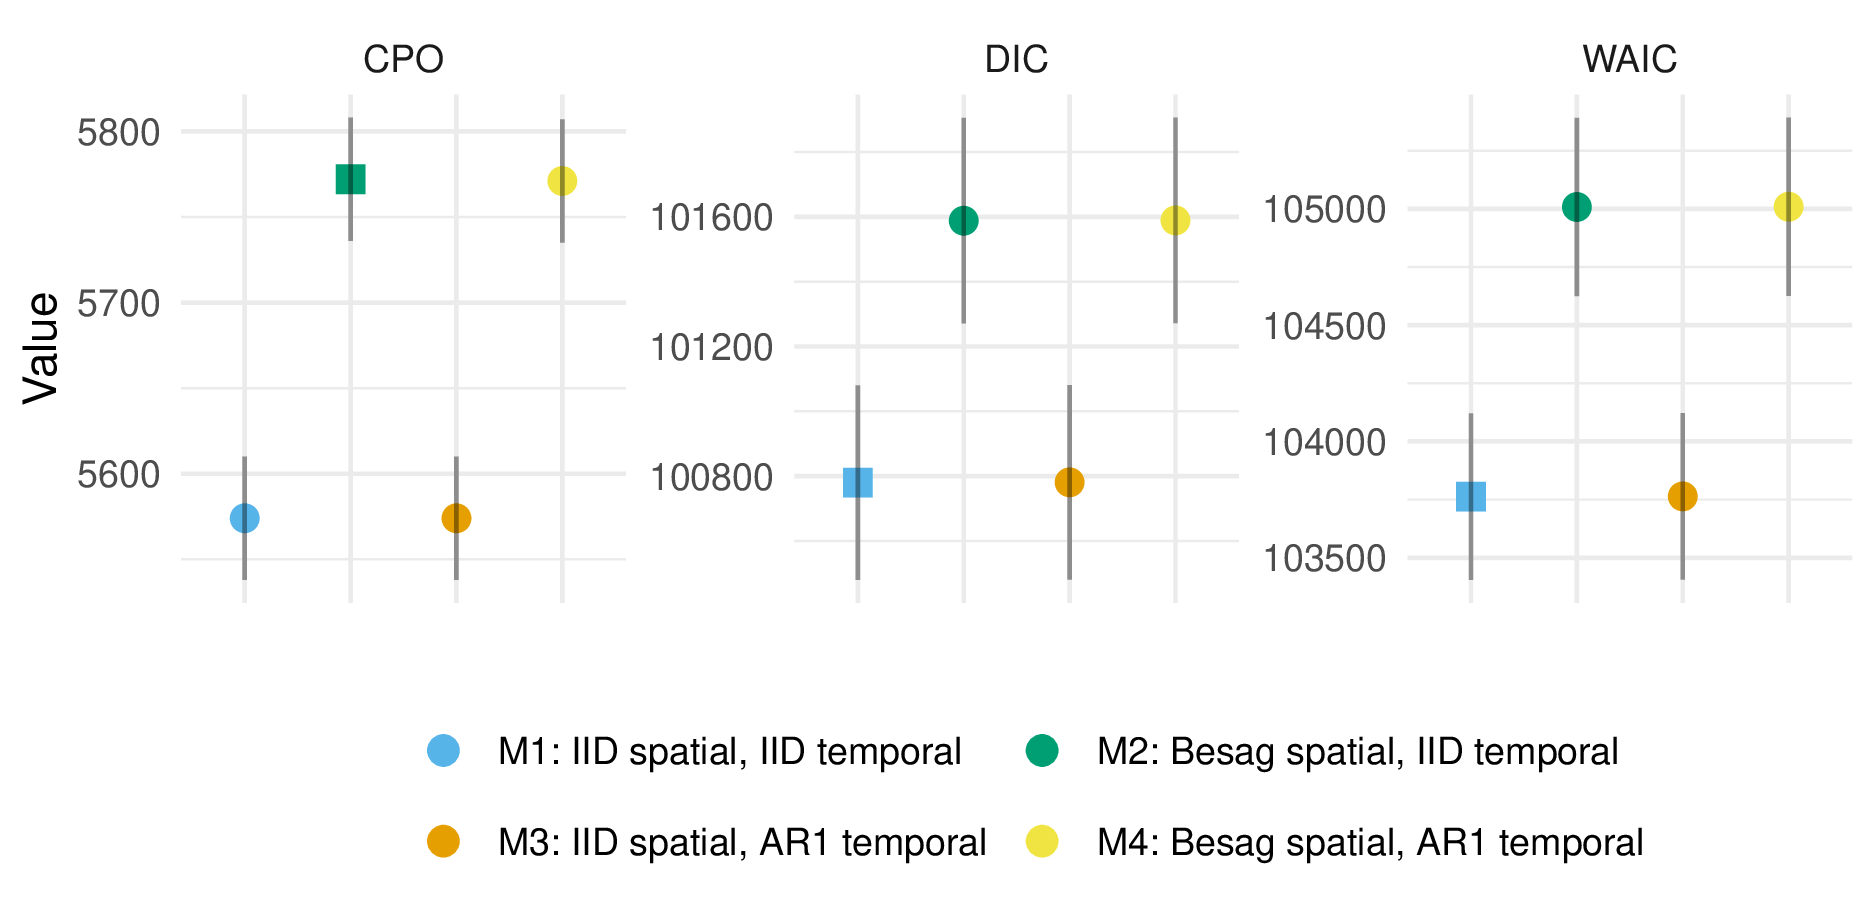
\includegraphics[width=0.95\linewidth]{resources/multi-agyw/20230627-144735-3da88508/depends/model-comparison} 

}

\caption{For the multinomial logistic regression model, under the CPO criterion, including Besag spatial random effects rather than IID spatial random effects improved model performance. On the other hand, under the DIC and WAIC, where smaller values are preferred, the opposite was true. Though IID temporal random effects are preferred by all criteria AR1 temporal random effects performed very similarly, likely as there is a limited amount of temporal variation in the data to describe.}\label{fig:model-comparison}
\end{figure}

\begin{longtable}[]{@{}lllll@{}}
\caption{\label{tab:model-comparison} CPO, DIC, and WAIC values for the multinomial logistic regression model with corresponding standard errors.}\tabularnewline
\toprule\noalign{}
& M1 & M2 & M3 & M4 \\
\midrule\noalign{}
\endfirsthead
\toprule\noalign{}
& M1 & M2 & M3 & M4 \\
\midrule\noalign{}
\endhead
\bottomrule\noalign{}
\endlastfoot
CPO & 5573 (36) & 5772 (36) & 5574 (36) & 5771 (36) \\
DIC & 100780 (300) & 101588 (317) & 100781 (300) & 101589 (317) \\
WAIC & 103763 (358) & 105008 (383) & 103763 (358) & 105009 (383) \\
\end{longtable}

\hypertarget{s-logistic}{%
\subsection{Spatial logistic regression}\label{s-logistic}}

To estimate the proportion of those in the \(k = 3^{+}\) risk group that were in the \(k = 3\) and \(k = 4\) risk groups respectively, I fit logistic regression models of the form
\begin{align}
    y_{ia4} &\sim \text{Binomial} \left( y_{ia3} + y_{ia4}, q_{ia} \right), \label{eq:logistic-regression} \\
    q_{ia} &= \text{logit}^{-1} \left( \eta_{ia} \right), 
\end{align}
where
\begin{equation}
q_{ia} = \frac{p_{ia4}}{p_{ia3} + p_{ia4}} = \frac{p_{ia4}}{p_{ia{3^+}}}.
\end{equation}
This two-step approach allowed all surveys to be included in the multinomial regression model, but only those surveys with a specific transactional sex question to be included in the logistic regression model.
As all such surveys occurred in the years 2013-2018 (Figure \ref{fig:available-surveys}), I assumed \(q_{ia}\) to be constant with respect to time.

\hypertarget{model-specifications-1}{%
\subsubsection{Model specifications}\label{model-specifications-1}}

\begin{longtable}[]{@{}
  >{\raggedright\arraybackslash}p{(\columnwidth - 10\tabcolsep) * \real{0.0241}}
  >{\raggedright\arraybackslash}p{(\columnwidth - 10\tabcolsep) * \real{0.2289}}
  >{\raggedright\arraybackslash}p{(\columnwidth - 10\tabcolsep) * \real{0.2289}}
  >{\raggedright\arraybackslash}p{(\columnwidth - 10\tabcolsep) * \real{0.2048}}
  >{\raggedright\arraybackslash}p{(\columnwidth - 10\tabcolsep) * \real{0.1928}}
  >{\raggedright\arraybackslash}p{(\columnwidth - 10\tabcolsep) * \real{0.1205}}@{}}
\caption{\label{tab:logistic-models} Six logistic regression models were considered. The covariate \texttt{cfswever} denotes the proportion of men who have ever paid for sex and \texttt{cfswrecent} denotes the proportion of men who have paid for sex in the past 12 months.}\tabularnewline
\toprule\noalign{}
\begin{minipage}[b]{\linewidth}\raggedright
\end{minipage} & \begin{minipage}[b]{\linewidth}\raggedright
Intercept \(\beta_0\)
\end{minipage} & \begin{minipage}[b]{\linewidth}\raggedright
Country \(\zeta_{c}\)
\end{minipage} & \begin{minipage}[b]{\linewidth}\raggedright
Age \(\alpha_{ac}\)
\end{minipage} & \begin{minipage}[b]{\linewidth}\raggedright
Spatial \(u_{i}\)
\end{minipage} & \begin{minipage}[b]{\linewidth}\raggedright
Covariates
\end{minipage} \\
\midrule\noalign{}
\endfirsthead
\toprule\noalign{}
\begin{minipage}[b]{\linewidth}\raggedright
\end{minipage} & \begin{minipage}[b]{\linewidth}\raggedright
Intercept \(\beta_0\)
\end{minipage} & \begin{minipage}[b]{\linewidth}\raggedright
Country \(\zeta_{c}\)
\end{minipage} & \begin{minipage}[b]{\linewidth}\raggedright
Age \(\alpha_{ac}\)
\end{minipage} & \begin{minipage}[b]{\linewidth}\raggedright
Spatial \(u_{i}\)
\end{minipage} & \begin{minipage}[b]{\linewidth}\raggedright
Covariates
\end{minipage} \\
\midrule\noalign{}
\endhead
\bottomrule\noalign{}
\endlastfoot
L1 & Constant & IID & IID & IID & None \\
L2 & Constant & IID & IID & Besag & None \\
L3 & Constant & IID & IID & IID & \texttt{cfswever} \\
L4 & Constant & IID & IID & Besag & \texttt{cfswever} \\
L5 & Constant & IID & IID & IID & \texttt{cfswrecent} \\
L6 & Constant & IID & IID & Besag & \texttt{cfswrecent} \\
\end{longtable}

I considered six logistic regression models (Table \ref{tab:logistic-models}).
Each included a constant intercept \(\beta_0 \sim \mathcal{N}(-2, 1^2)\), country random effects \(\zeta_{c} \sim \mathcal{N}(0, \tau_\zeta^{-1})\), and age-country random effects \(\alpha_{ac} \sim \mathcal{N}(0, \tau_\alpha^{-1})\).
The Gaussian prior distribution on \(\beta_0\) placed 95\% prior probability on the range 2-50\% for the percentage of those with non-regular or multiple partners who report transactional sex.
I considered two specifications (IID, Besag) for the spatial random effects \(u_i\).
To aid estimation with sparse data, I also considered national-level covariates for the proportion of men who have paid for sex ever \texttt{cfswever} or in the last twelve months \texttt{cfswrecent} \autocite{hodgins2022population}.
For both random effect precision parameters \(\tau \in \{\tau_\alpha, \tau_\zeta\}\) I used the PC prior distribution with base model \(\sigma = 0\) and \(\mathbb{P}(\sigma > 2.5 = 0.01)\).
For both regression parameters \(\beta \in \{\beta_\texttt{cfswever}, \beta_\texttt{cfswrecent}\}\) I used the prior distribution \(\beta \sim \mathcal{N}(0, 2.5^2)\).

\hypertarget{survey-weighted-likelihood-1}{%
\subsubsection{Survey weighted likelihood}\label{survey-weighted-likelihood-1}}

As with the multinomial regression model, I used survey weighted counts \(y^\star\) and sample sizes \(m^\star\).
I used a generalised binomial pseudo-likelihood \(y^\star \sim \text{xBinomial}(m^\star, q)\) given by
\begin{equation}
    p(y^\star \, | \, m^\star, q) =  \binom{\lfloor m^\star \rfloor}{\lfloor y^\star \rfloor} q^{y^\star} (1 - q)^{m^\star - y^\star}
\end{equation}
to extend the binomial distribution to non-integer weighted counts and sample sizes.
This working likelihood is implemented by \texttt{family\ =\ "xBinomial"} in \texttt{R-INLA}.

\hypertarget{model-selection-1}{%
\subsubsection{Model selection}\label{model-selection-1}}

I selected the model including Besag spatial effects and \texttt{cfswrecent} covariates according to the CPO criterion.
All results, including DIC and WAIC, are presented in Table and Figure \ref{fig:fsw-logit-model-comparison}.
Inclusion of Besag spatial random effects, rather than IID, consistently improved performance.
Benefits from inclusion of covariates were more marginal.
As some countries had no suitable surveys, I nonetheless preferred to include covariate information so that estimates in these countries would be based on some country-specific data.



\begin{figure}

{\centering 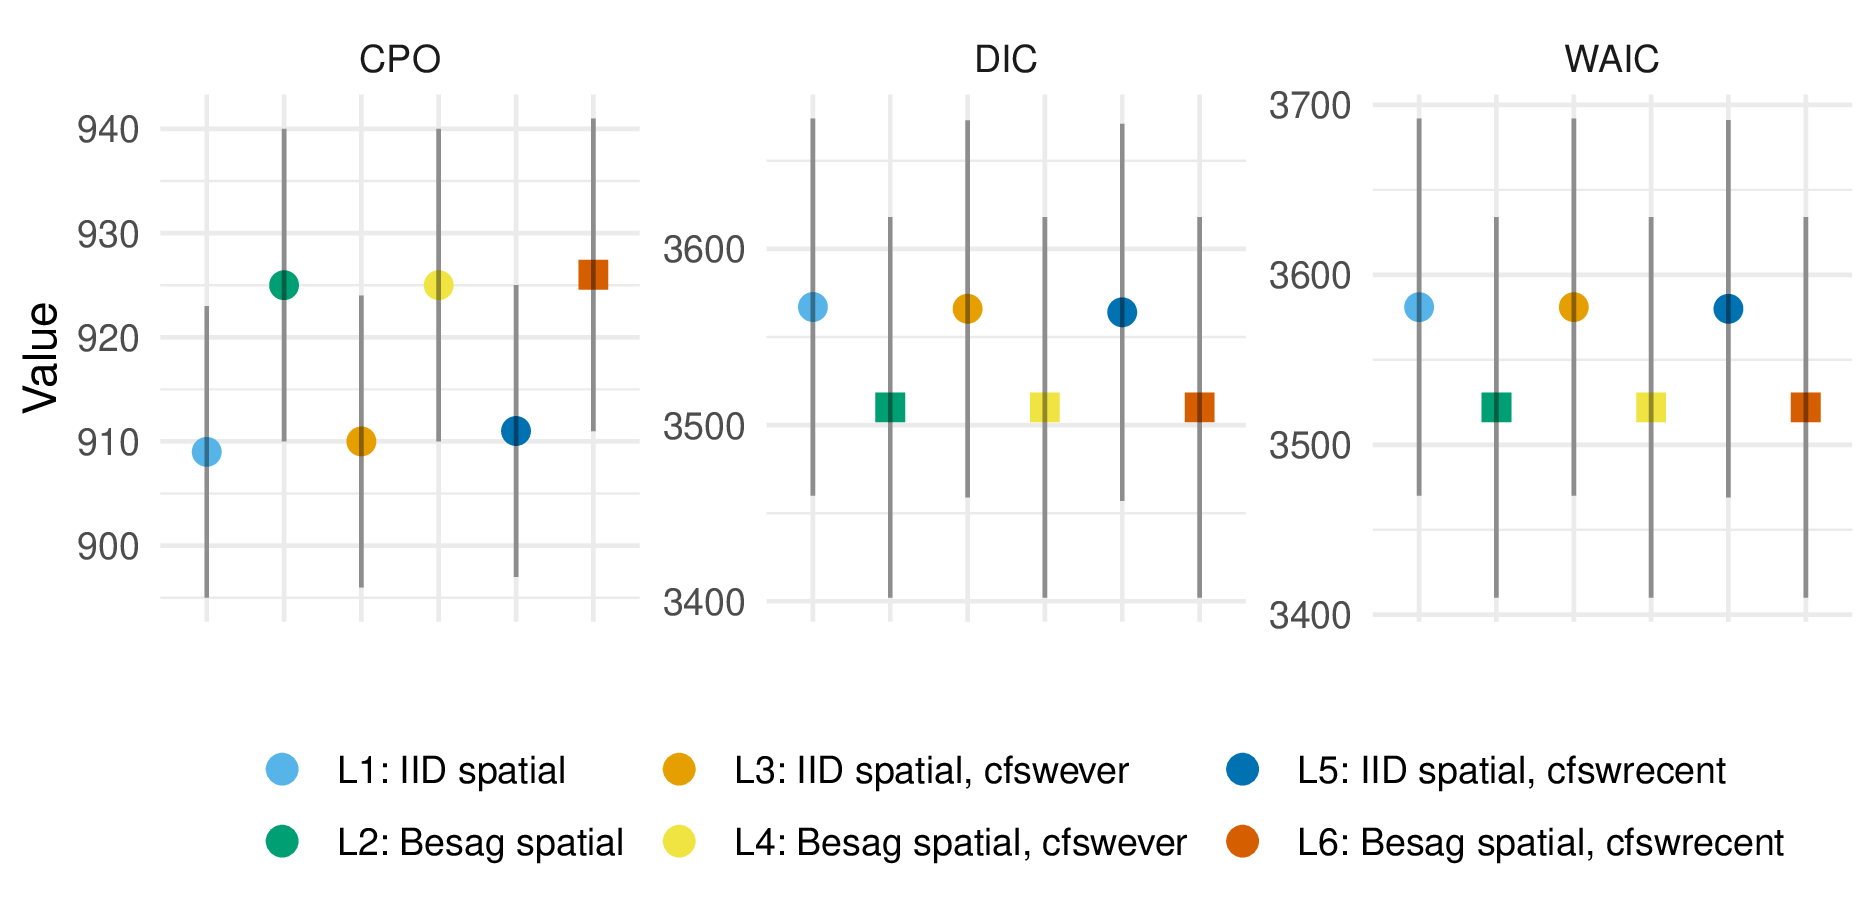
\includegraphics[width=0.95\linewidth]{resources/multi-agyw/20230627-144735-3da88508/depends/fsw-logit-model-comparison} 

}

\caption{For the logistic regression model, the CPO, DIC, and WAIC each agreed that the model containing Besag spatial random effects and the \texttt{csfwrecent} covariates was best. Inclusion of Besag spatial random effects consistently improved each criterion, whereas improvements from inclusion of any covariates were marginal.}\label{fig:fsw-logit-model-comparison}
\end{figure}

\begin{longtable}[]{@{}
  >{\raggedright\arraybackslash}p{(\columnwidth - 12\tabcolsep) * \real{0.0769}}
  >{\raggedright\arraybackslash}p{(\columnwidth - 12\tabcolsep) * \real{0.1538}}
  >{\raggedright\arraybackslash}p{(\columnwidth - 12\tabcolsep) * \real{0.1538}}
  >{\raggedright\arraybackslash}p{(\columnwidth - 12\tabcolsep) * \real{0.1538}}
  >{\raggedright\arraybackslash}p{(\columnwidth - 12\tabcolsep) * \real{0.1538}}
  >{\raggedright\arraybackslash}p{(\columnwidth - 12\tabcolsep) * \real{0.1538}}
  >{\raggedright\arraybackslash}p{(\columnwidth - 12\tabcolsep) * \real{0.1538}}@{}}
\caption{\label{tab:model-comparison} CPO, DIC, and WAIC values for the logistic regression model with corresponding standard errors.}\tabularnewline
\toprule\noalign{}
\begin{minipage}[b]{\linewidth}\raggedright
\end{minipage} & \begin{minipage}[b]{\linewidth}\raggedright
L1
\end{minipage} & \begin{minipage}[b]{\linewidth}\raggedright
L2
\end{minipage} & \begin{minipage}[b]{\linewidth}\raggedright
L3
\end{minipage} & \begin{minipage}[b]{\linewidth}\raggedright
L4
\end{minipage} & \begin{minipage}[b]{\linewidth}\raggedright
L5
\end{minipage} & \begin{minipage}[b]{\linewidth}\raggedright
L6
\end{minipage} \\
\midrule\noalign{}
\endfirsthead
\toprule\noalign{}
\begin{minipage}[b]{\linewidth}\raggedright
\end{minipage} & \begin{minipage}[b]{\linewidth}\raggedright
L1
\end{minipage} & \begin{minipage}[b]{\linewidth}\raggedright
L2
\end{minipage} & \begin{minipage}[b]{\linewidth}\raggedright
L3
\end{minipage} & \begin{minipage}[b]{\linewidth}\raggedright
L4
\end{minipage} & \begin{minipage}[b]{\linewidth}\raggedright
L5
\end{minipage} & \begin{minipage}[b]{\linewidth}\raggedright
L6
\end{minipage} \\
\midrule\noalign{}
\endhead
\bottomrule\noalign{}
\endlastfoot
DIC & 4662 (110) & 4605 (111) & 4662 (110) & 4605 (111) & 4662 (110) & 4605 (111) \\
WAIC & 4692 (115) & 4624 (115) & 4692 (115) & 4624 (115) & 4692 (115) & 4624 (115) \\
CPO & 950 (15) & 969 (15) & 951 (15) & 970 (15) & 950 (15) & 970 (15) \\
\end{longtable}

\hypertarget{model-combination}{%
\subsection{Model combination}\label{model-combination}}

How were the models combined?
Using samples.

\hypertarget{female-sex-worker-population-size-adjustment}{%
\subsection{Female sex worker population size adjustment}\label{female-sex-worker-population-size-adjustment}}

Having had sex ``in return for gifts, cash or anything else in the past 12 months'' is not considered sufficient to constitute sex work.
As such, I adjusted the estimates obtained based on the transactional sex survey question to match FSW population size estimates obtained using an alternative method, which I describe below.
The estimates of the non-regular or multiple sexual partner(s) population size were changed to facilitate changing of the FSW population size.
This approach retained subnational variation informed by the transactional sex survey question.

I used the estimates adult (15-49) FSW population size by country from a Bayesian meta-analysis of key population specific data sources \autocite{stevens2022estimating}.
To disaggregate these estimates by age, I took the following steps.
First, I calculated the total sexually debuted population in each age group, by country.
To describe the distribution of age at first sex, I used skew logistic distributions \autocite{nguyen2022trends} with cumulative distribution function given by
\begin{equation}
F(x) = \left(1 + \exp(\kappa_c (\mu_c - x)) \right)^{- \gamma_c},
\end{equation}
where \(\kappa_c, \mu_c, \gamma_c > 0\) are country-specific shape, shape and skewness parameters respectively.
Next, I used the assumed \(\text{Gamma}(\alpha = 10.4, \beta = 0.36)\) FSW age distribution in South Africa from the Thembisa model \autocite{johnson2020thembisa} to calculate the implied ratio between the number of FSW and the sexually debuted population in each age group.
I assumed the South African ratios were applicable to every country, allowing calculation of the number of FSW by age group in all 13 countries.
The resulting age trends obtained (Figure \ref{fig:age-disagg-fsw-line}) reflect country-level variation in demographics and age-at-first-sex.



\begin{figure}

{\centering 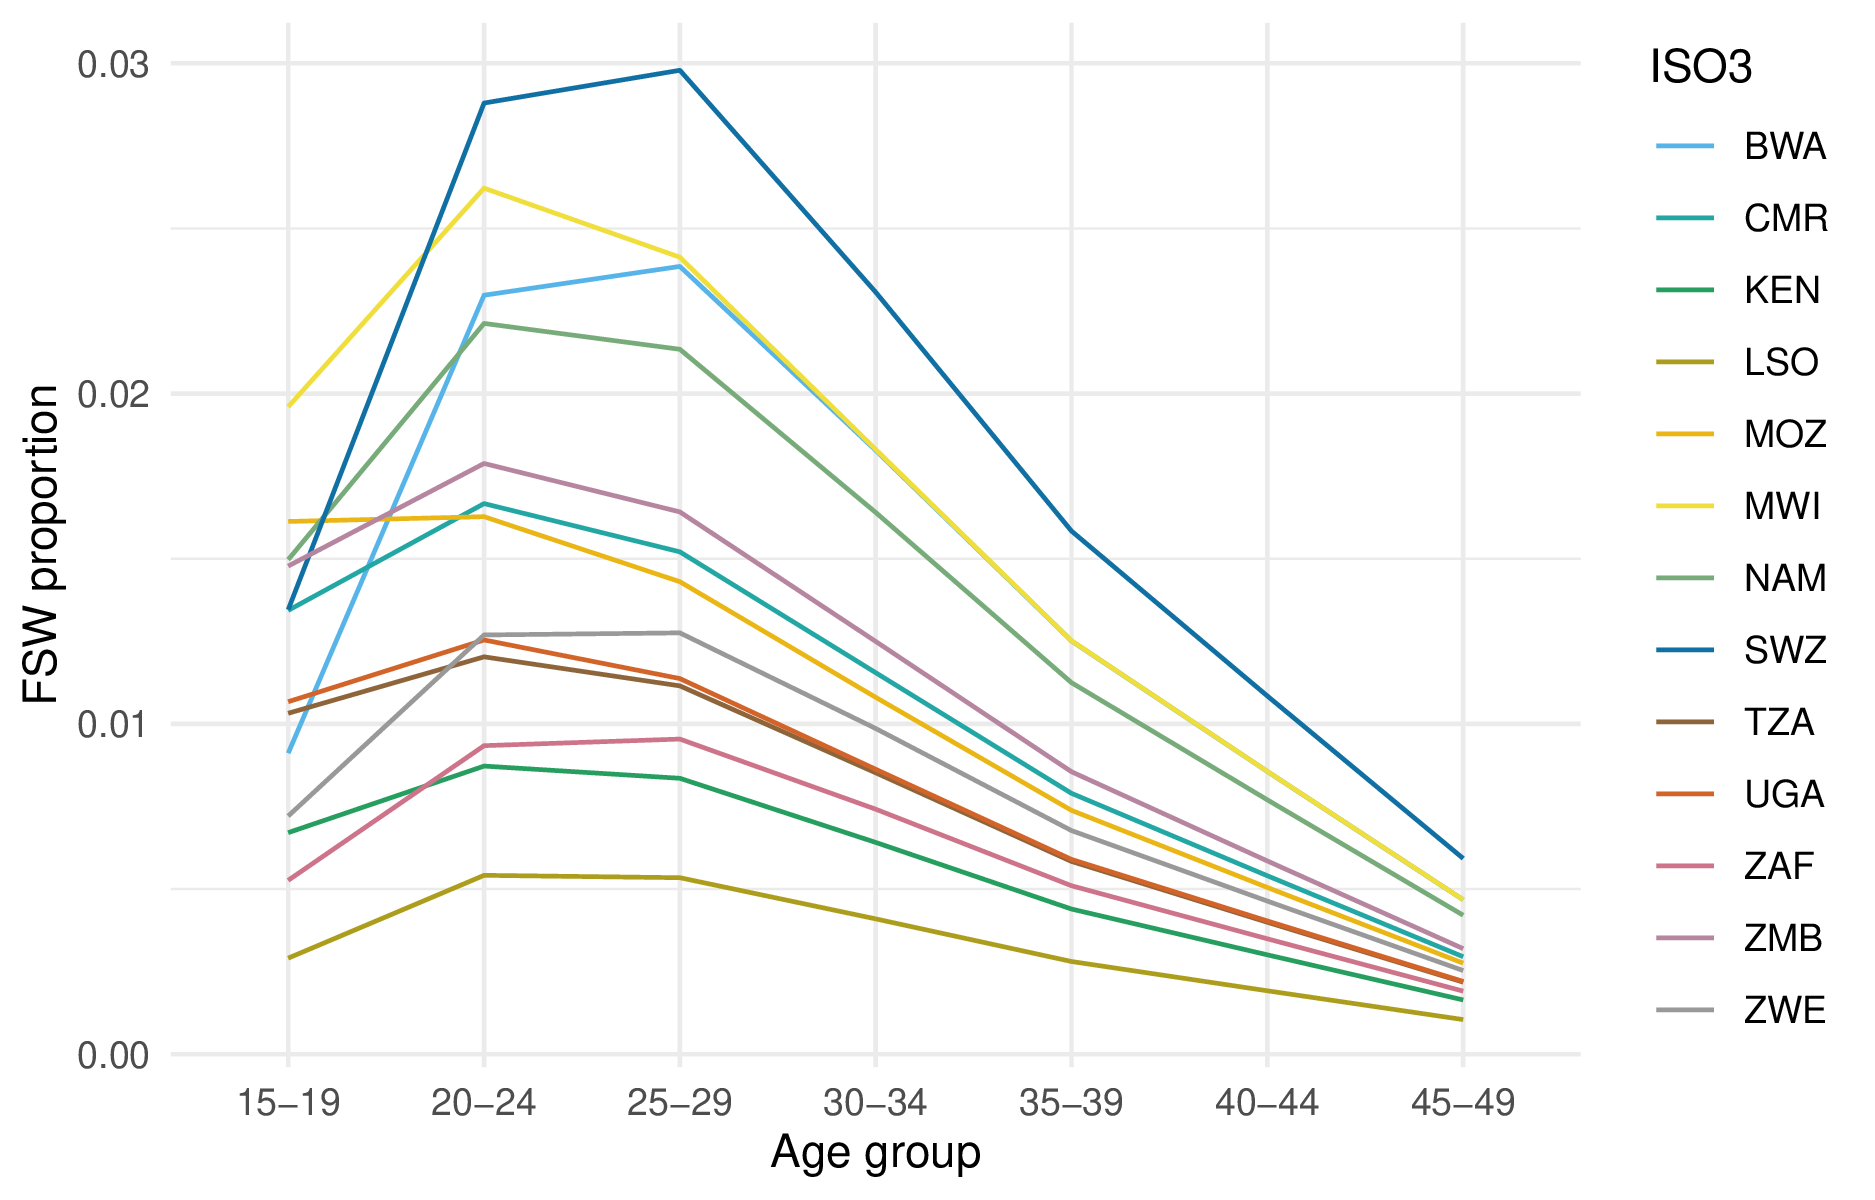
\includegraphics[width=0.95\linewidth]{resources/multi-agyw/20230627-144735-3da88508/depends/age-disagg-fsw-line} 

}

\caption{The disaggregation procedure I used produces an age distribution for FSW peaking in the 20-24 and 25-29 age groups, and declining for older age groups.}\label{fig:age-disagg-fsw-line}
\end{figure}

\hypertarget{results}{%
\subsection{Results}\label{results}}

\hypertarget{coverage-assessment}{%
\subsubsection{Coverage assessment}\label{coverage-assessment}}

To assess the calibration of the fitted model, I calculated the quantile \(q\) of each observation within the posterior predictive distribution.
For calibrated models, these quantiles, known as probability integral transform (PIT) values \autocite{dawid1984present,bosse2022scoringutils}, should follow a uniform distribution \(q \sim \mathcal{U}[0, 1]\).
To generate samples from the posterior predictive distribution, I applied the multinomial likelihood to samples from the latent field, setting the sample size to be the floor of the Kish effective sample size.
Using the PIT values, it is possible to calculate the empirical coverage of all \((1 - \alpha)100\)\% equal-tailed posterior predictive credible intervals.
These empirical coverages can be compared to the nominal coverage \((1 - \alpha)\) for each value of \(\alpha \in [0, 1]\) to give empirical cumulative distribution function (ECDF) difference values.
This approach has the advantage of considering all possible confidence values at once.
To test for uniformity, I used the binomial distribution based simultaneous confidence bands for ECDF difference values developed by \textcite{sailynoja2021graphical}.
I found the only significant deviation from uniformity occurred in the right-hand tail of the one cohabiting partner risk group.
That is to say, the proportion of the PIT values which were greater than 0.95 was significantly more than would be expected under a calibrated model.



\begin{figure}

{\centering 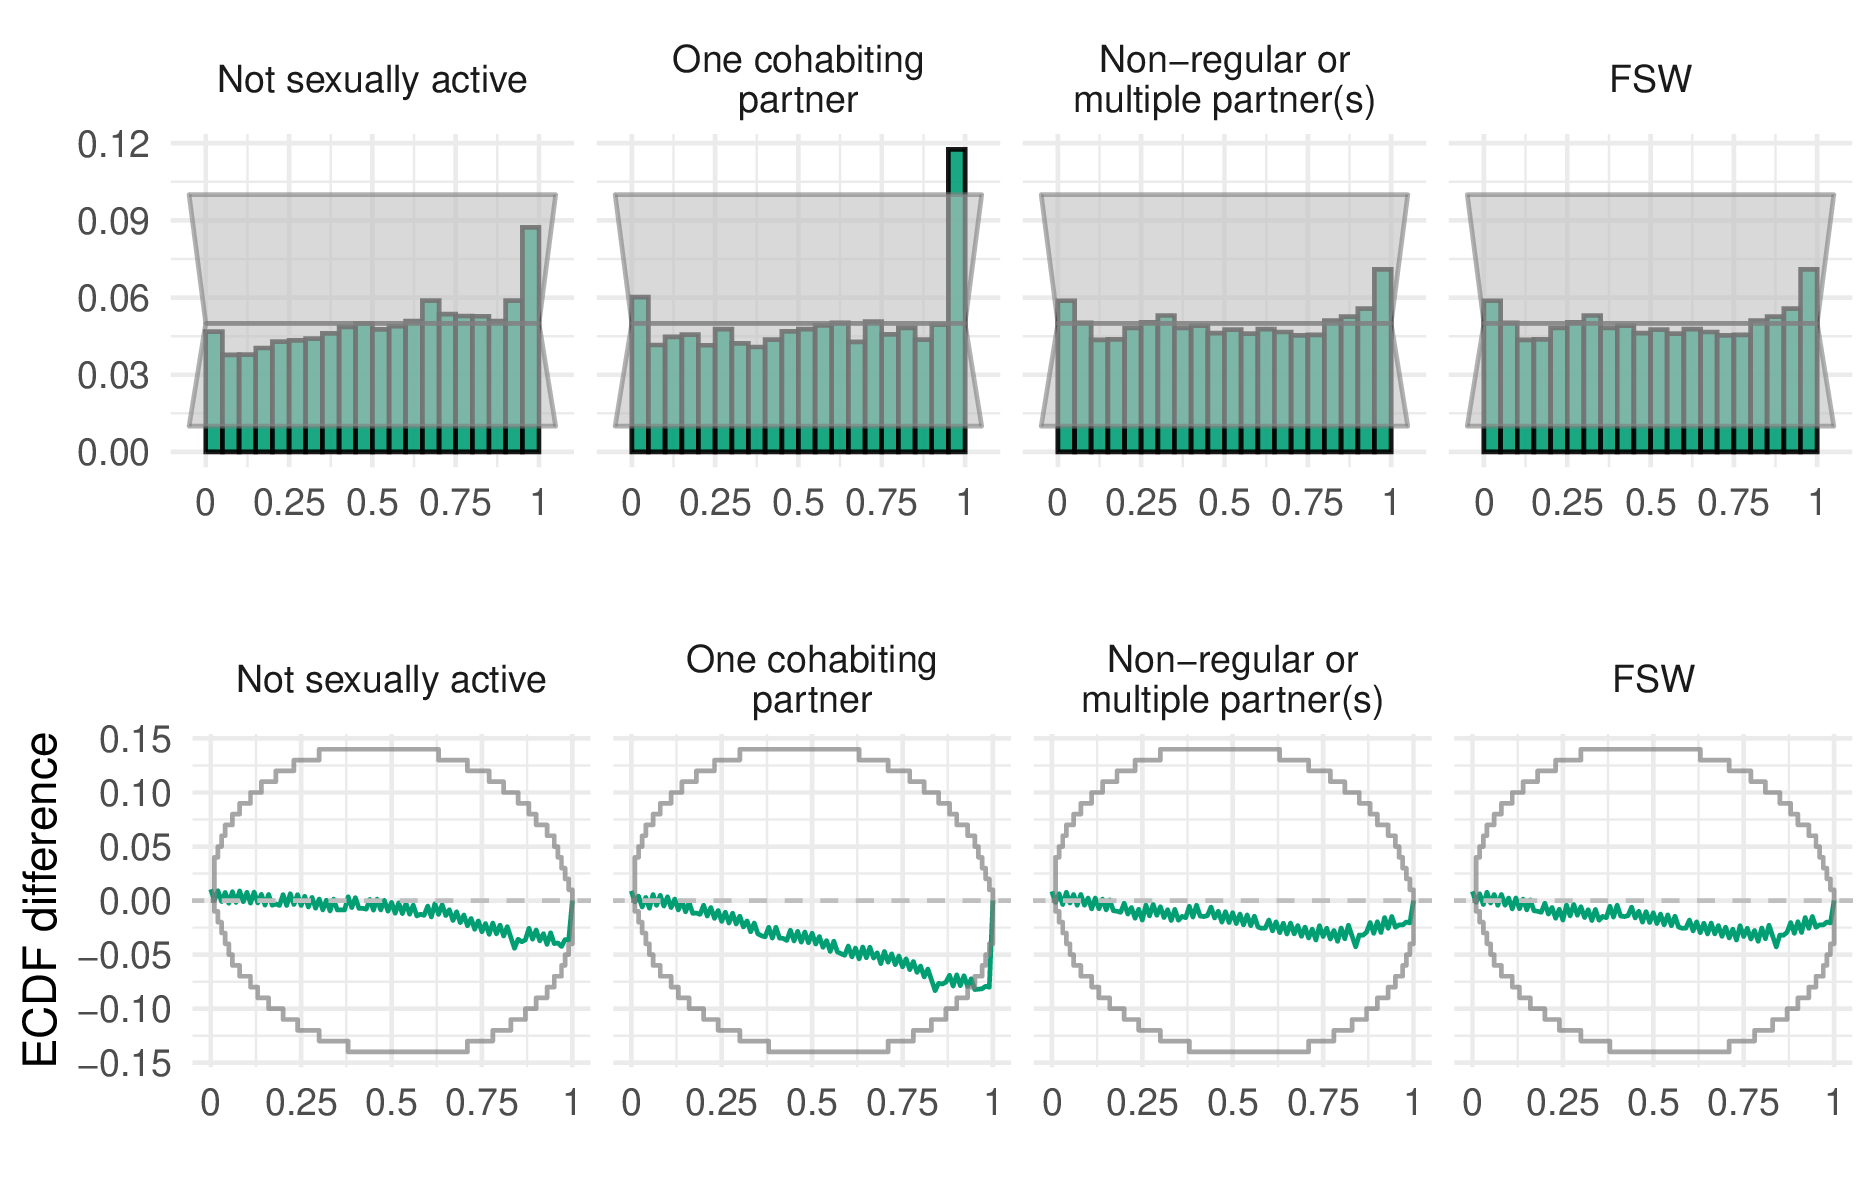
\includegraphics[width=0.95\linewidth]{resources/multi-agyw/20230627-144735-3da88508/depends/coverage} 

}

\caption{Probability integral transform (PIT) histograms (top row) and empirical cumulative distribution function (ECDF) difference plots (bottom row) for the final selected model.}\label{fig:coverage}
\end{figure}

\hypertarget{estimates}{%
\subsubsection{Estimates}\label{estimates}}

Figure \ref{fig:aaa-variance-proportions} and Figure \ref{fig:3p1-within-between-country-variation} show posterior mean estimates for the proportion in each risk group for the final model in 2018, the most recent year included in our analysis.
I focused on the most recent estimates because they are the most relevant to inform ongoing HIV policy.
In subsequent results, all estimates refer to 2018, unless otherwise indicated.



\begin{figure}

{\centering 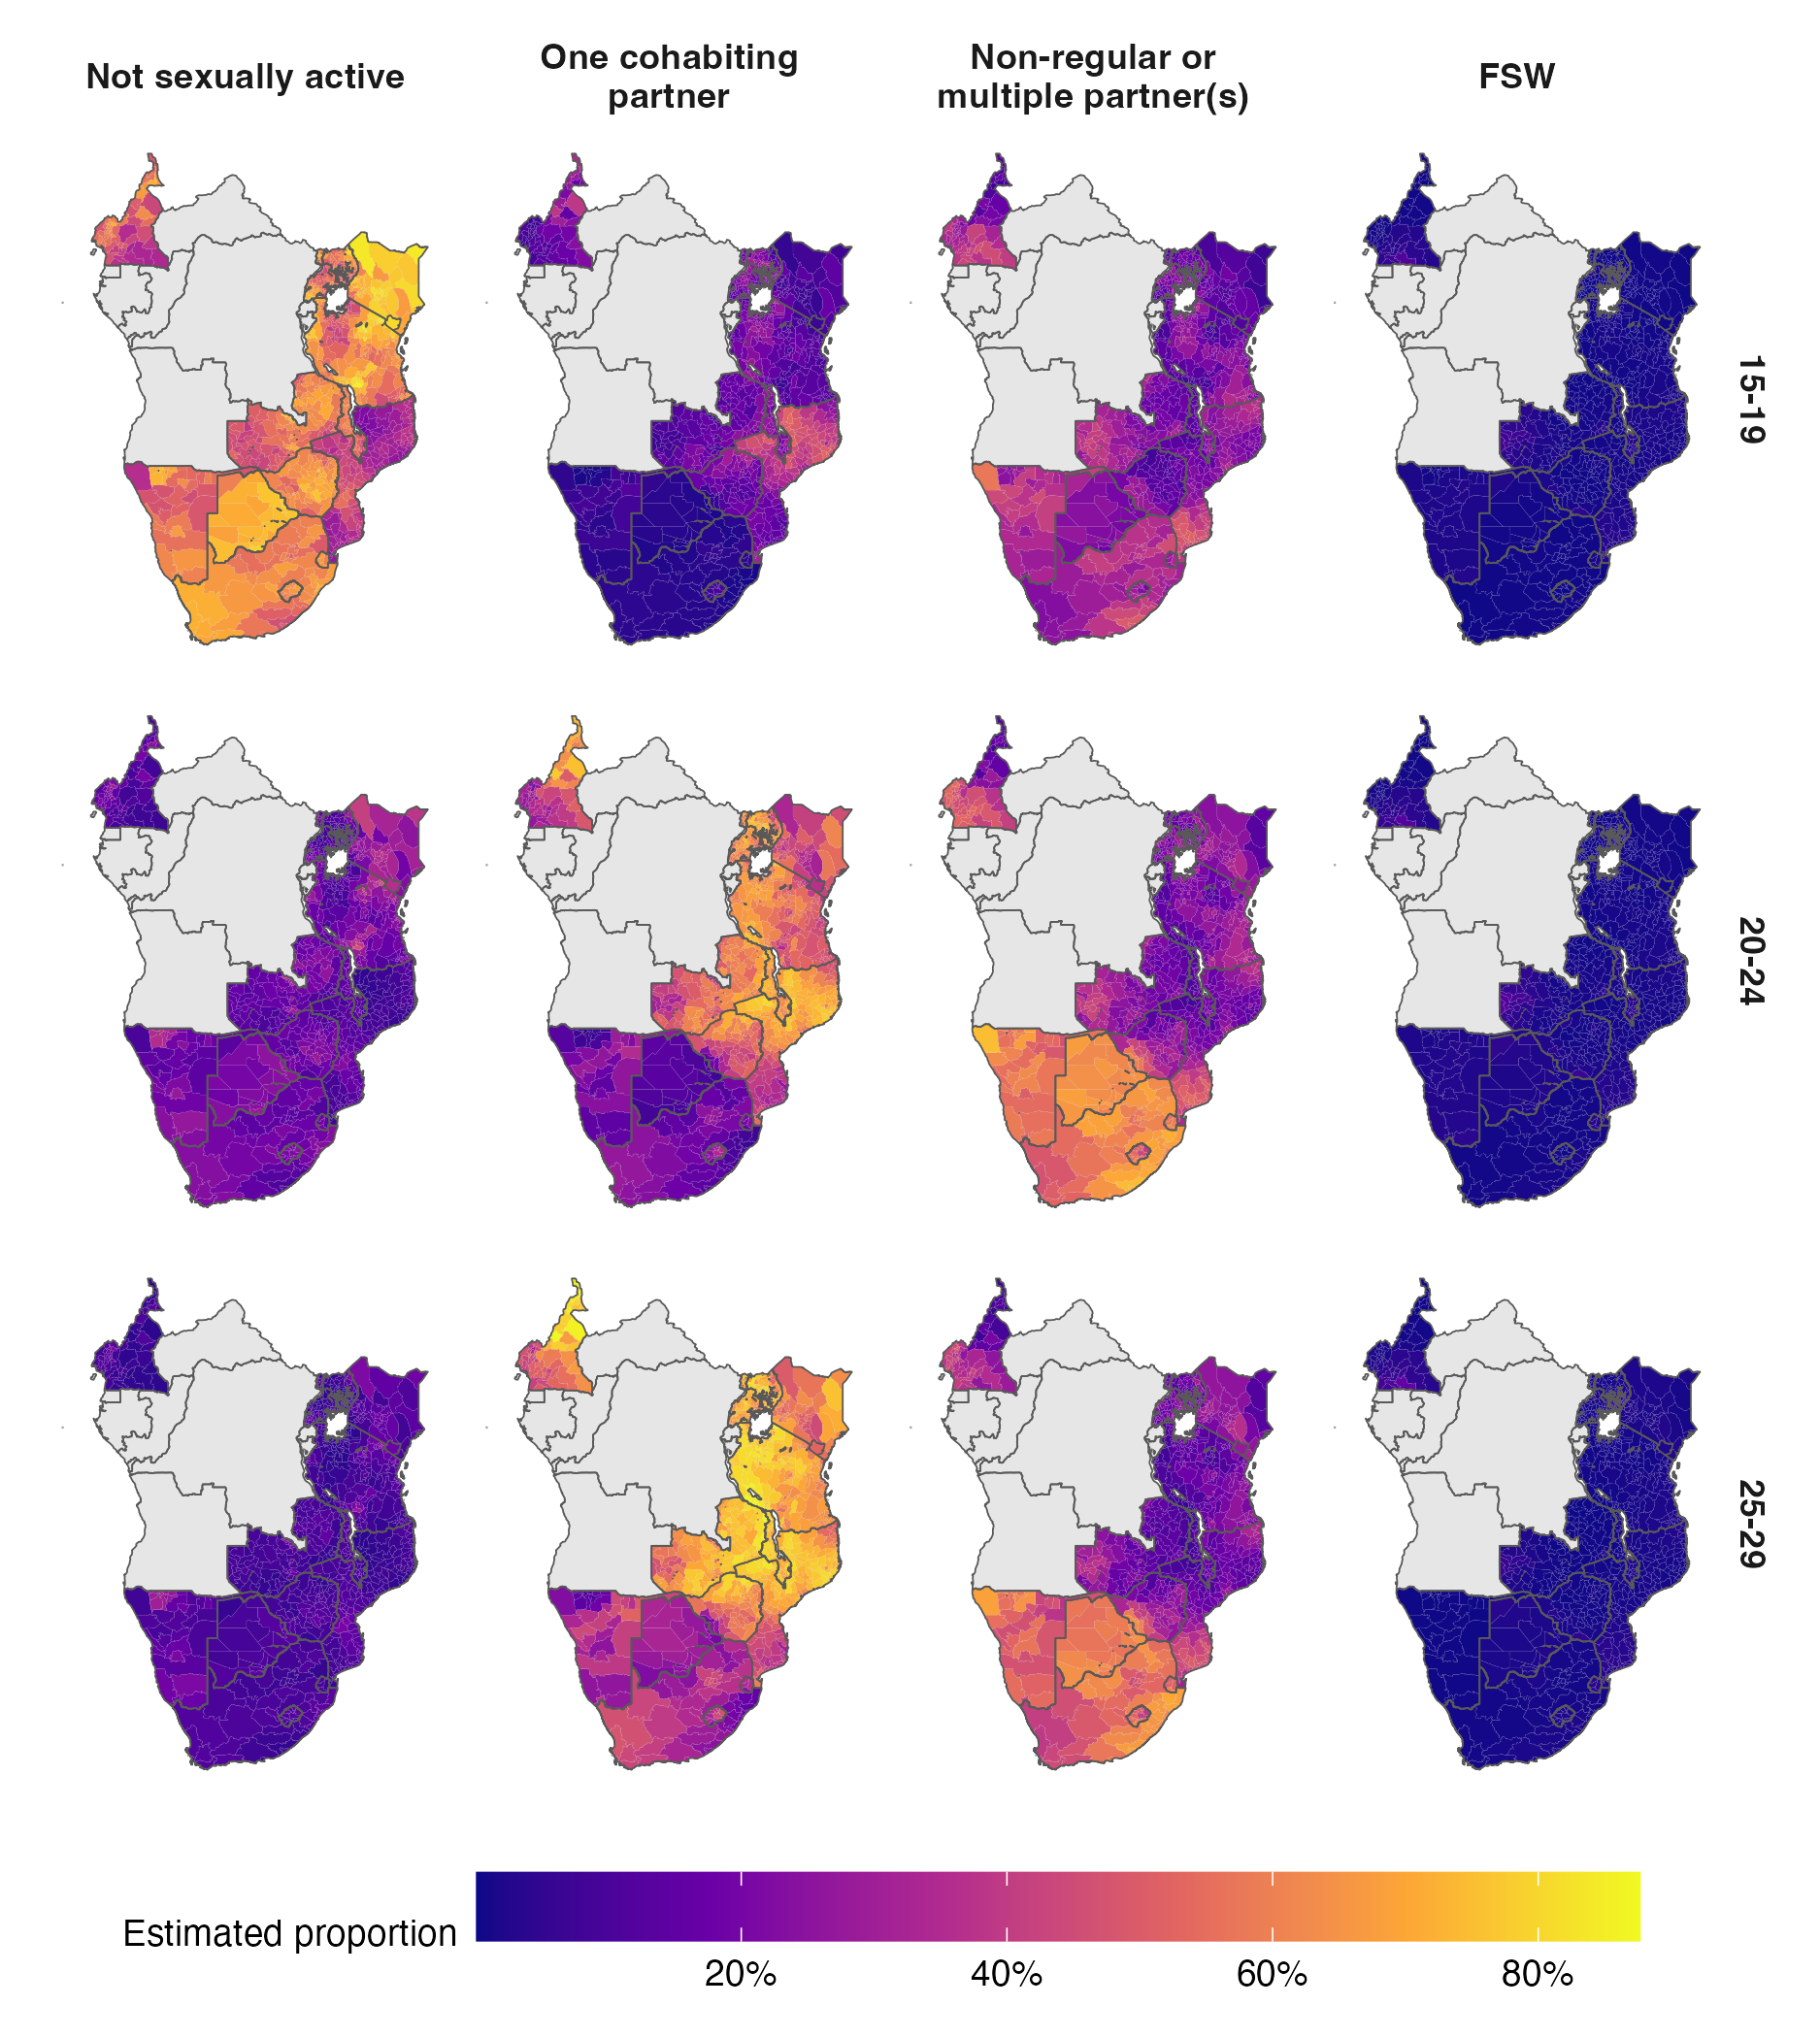
\includegraphics[width=0.95\linewidth]{resources/multi-agyw/20230627-144735-3da88508/depends/3p1-continental-map} 

}

\caption{The spatial distribution (posterior mean) of the AGYW risk group proportions in 2018. Estimates are stratified by risk group (columns) and five-year age group (rows). Countries in grey were not included in the analysis. A limitation of this figure is that using a common colour scale, desirable for other reasons, makes it challenging to see spatial variation in the FSW risk group.}\label{fig:3p1-continental-map}
\end{figure}



\begin{figure}

{\centering 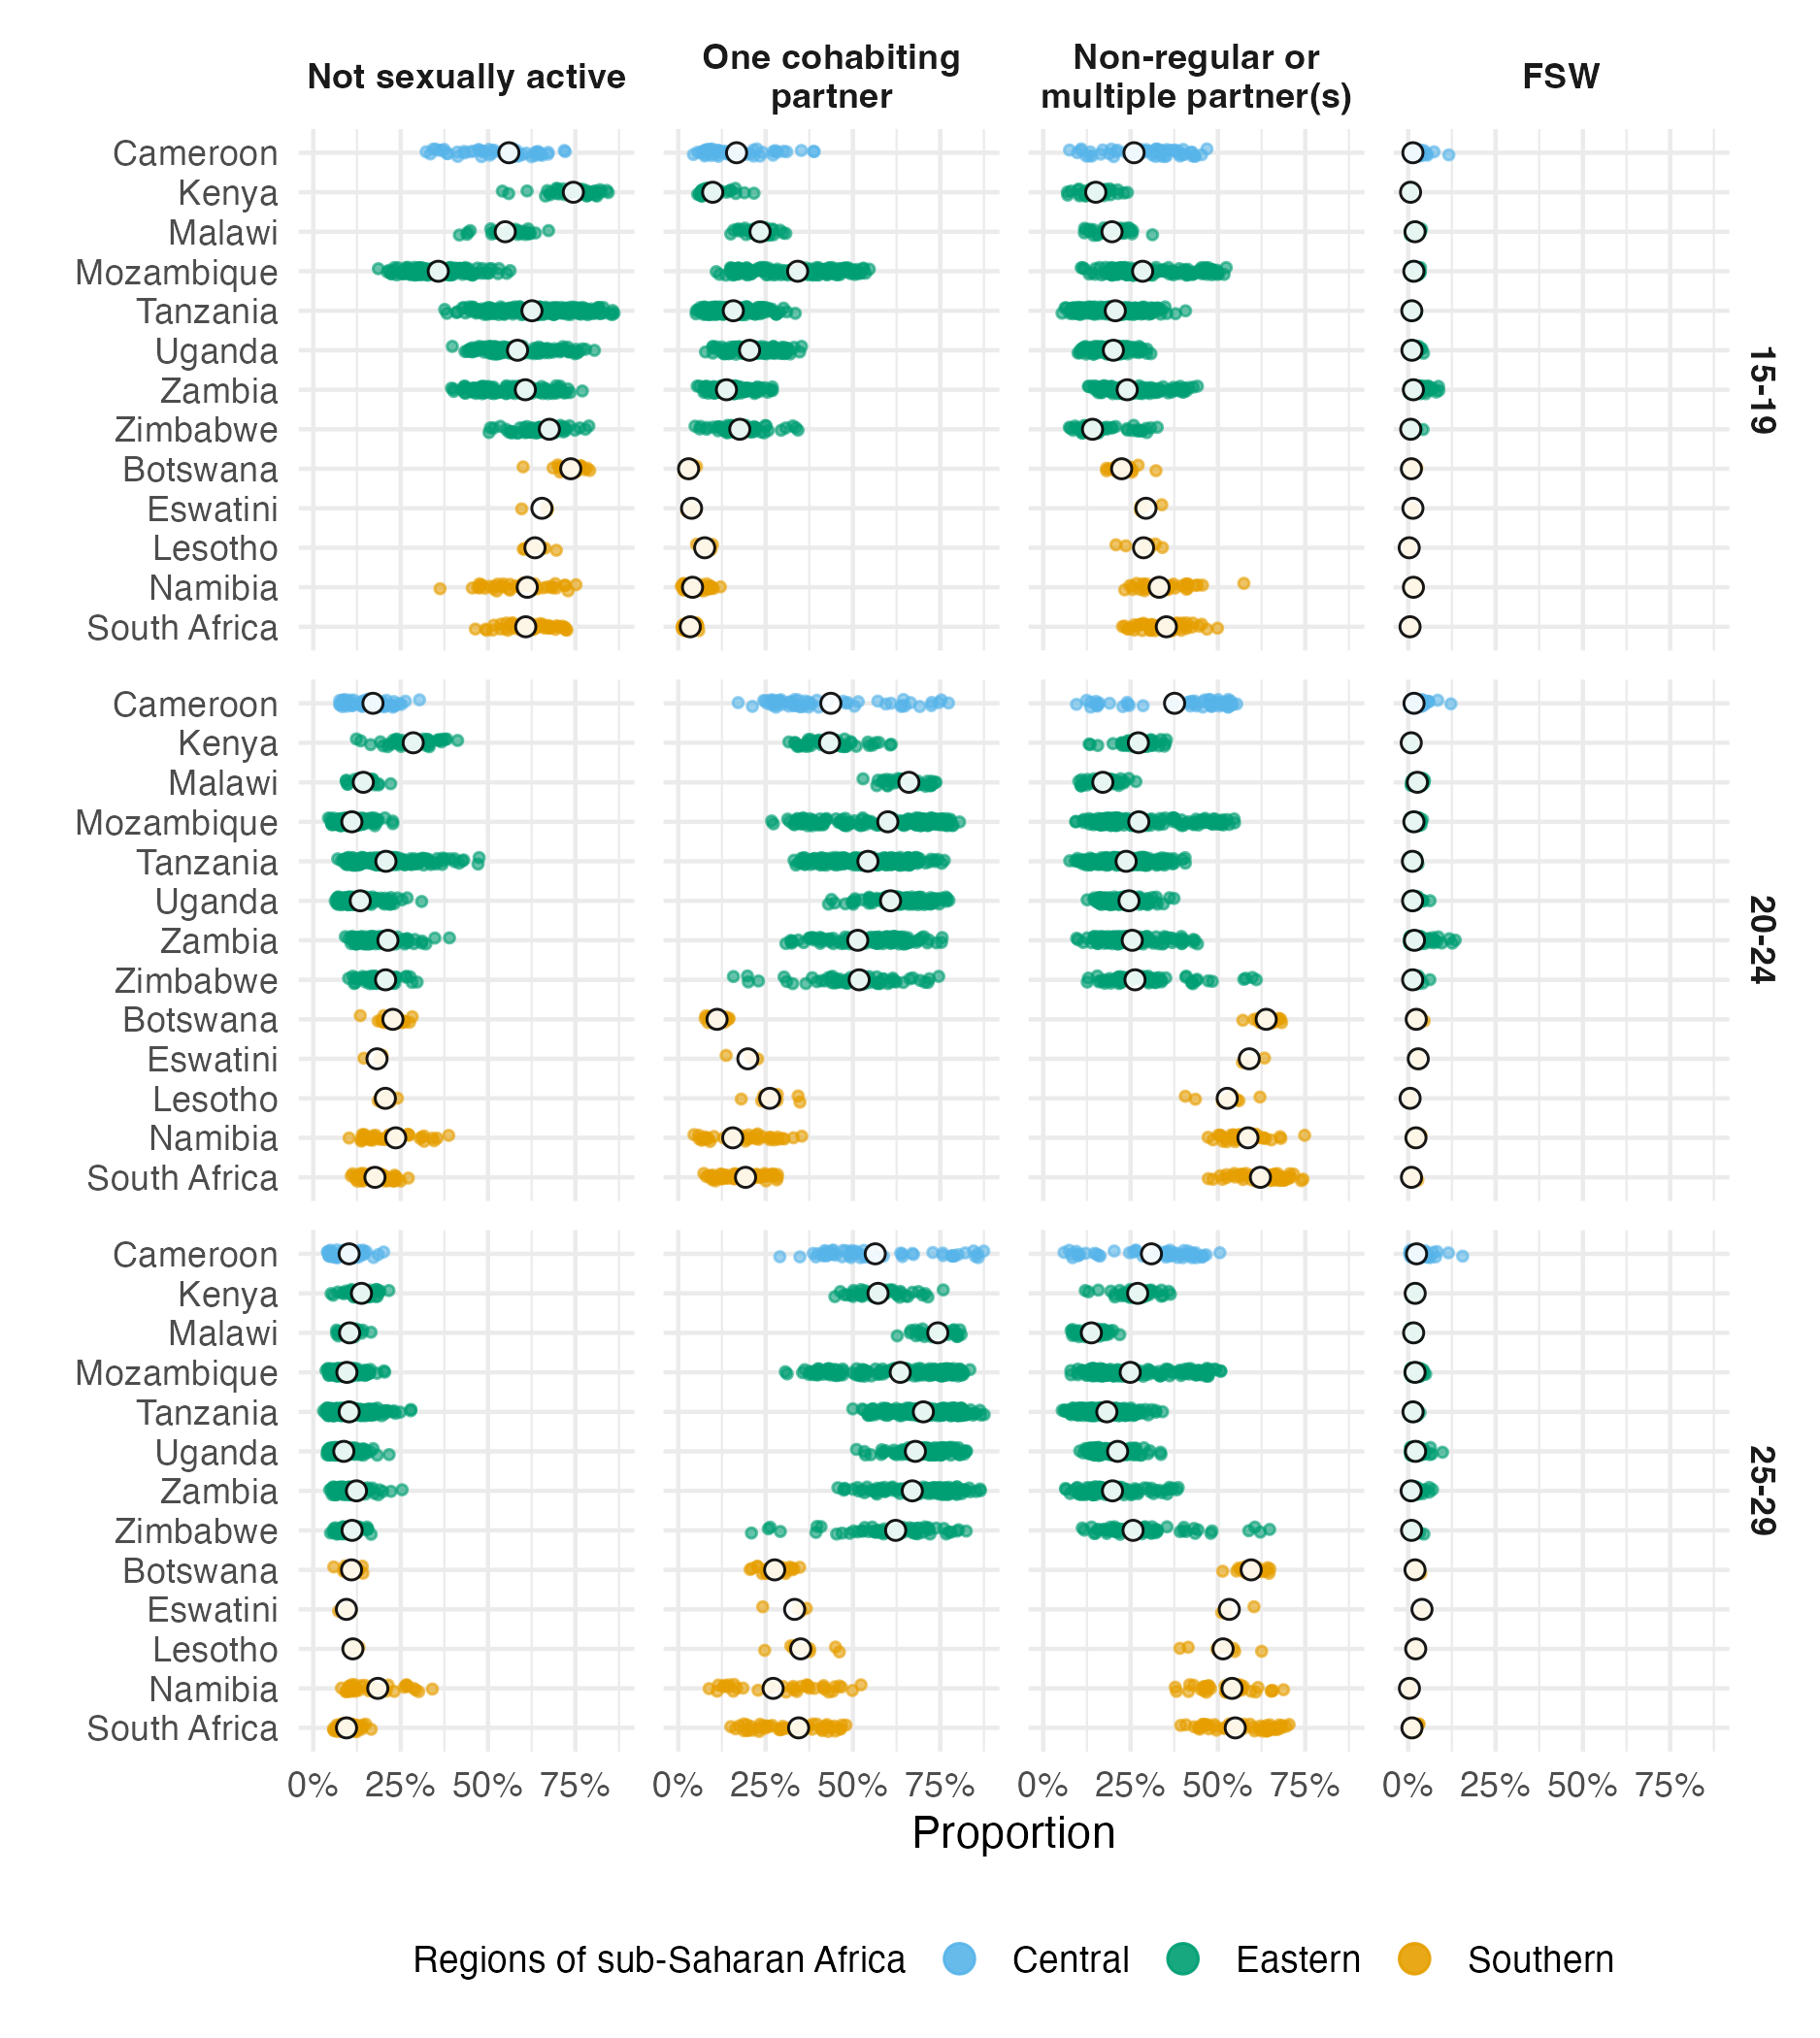
\includegraphics[width=0.95\linewidth]{resources/multi-agyw/20230627-144735-3da88508/depends/3p1-within-between-country-variation} 

}

\caption{National (in white) and subnational (in color) posterior means of the risk group proportions. Estimates are stratified by risk group (columns) and five-year age group (rows). Though the information presented is similar to that of Figure \ref{fig:3p1-continental-map}, this figure presents a clear view of within- and between-country variation in risk group proportions.}\label{fig:3p1-within-between-country-variation}
\end{figure}

The median national FSW proportion was 1.1\% (95\% CI 0.4--1.9) for the 15-19 age group, 1.6\% (95\% CI 0.6--2.8) for the 20-24 age group and 1.9\% (95\% CI 0.5--3.5) for the 25-29 age group, in line with the results displayed in Figure \ref{fig:age-disagg-fsw-line}.



\begin{figure}

{\centering 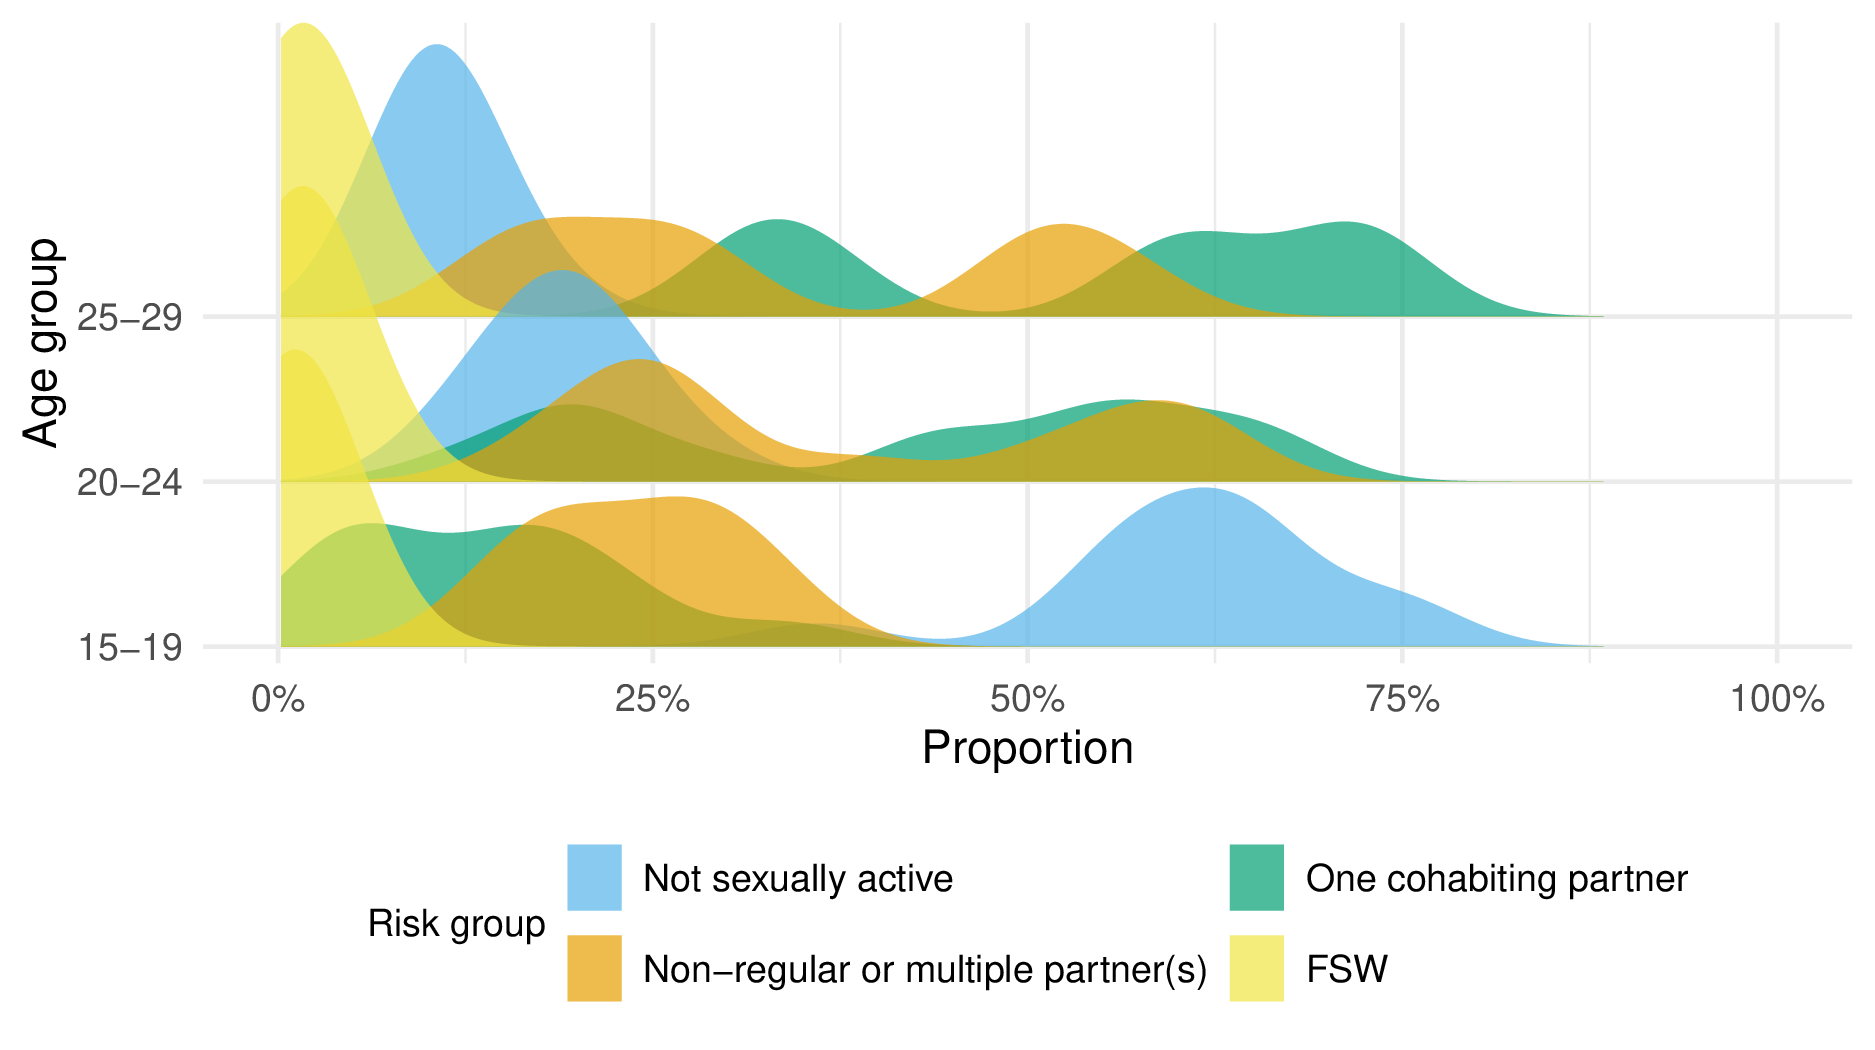
\includegraphics[width=0.95\linewidth]{resources/multi-agyw/20230627-144735-3da88508/depends/age-variation} 

}

\caption{Figure caption.}\label{fig:age-variation}
\end{figure}

In the 20-24 and 25-29 year age groups, the majority of women were either cohabiting or had non-regular or multiple partner(s).
Countries in eastern and central Africa (Cameroon, Kenya, Malawi, Mozambique, Tanzania, Uganda, Zambia and Zimbabwe) had a higher proportion of women in these age groups cohabiting (63.1\% {[}95\% CI 35--78.7\%{]} compared with 21.3\% {[}95\% CI 10.1--48.8\%{]} with non-regular partner{[}s{]}).
In contrast, countries in southern Africa (Botswana, Eswatini, Lesotho, Namibia and South Africa) had a higher proportion with non-regular or multiple partner(s) (58.9\% {[}95\% CI 43.2--70.5\%{]}, compared with 23.4\% {[}95\% CI 9.7--39.1\%{]} cohabiting).
This finding is the most notable feature of between-country variation shown in Figure \ref{fig:3p1-within-between-country-variation}.
Figure \ref{fig:3p1-continental-map} shows the geographic delineation to pass along the border of Mozambique, through the interior of Zimbabwe and along the border of Zambia.

In most districts (57.9\%; 95\% credible interval {[}CI{]} 27.7--79.7) adolescent girls aged 15-19 were not sexually active.
The exception was Mozambique, where the majority (64.23\%) were sexually active in the past year and close to a third (34.17\%) were cohabiting with a partner.

\hypertarget{variance-decomposition}{%
\subsubsection{Variance decomposition}\label{variance-decomposition}}



\begin{figure}

{\centering 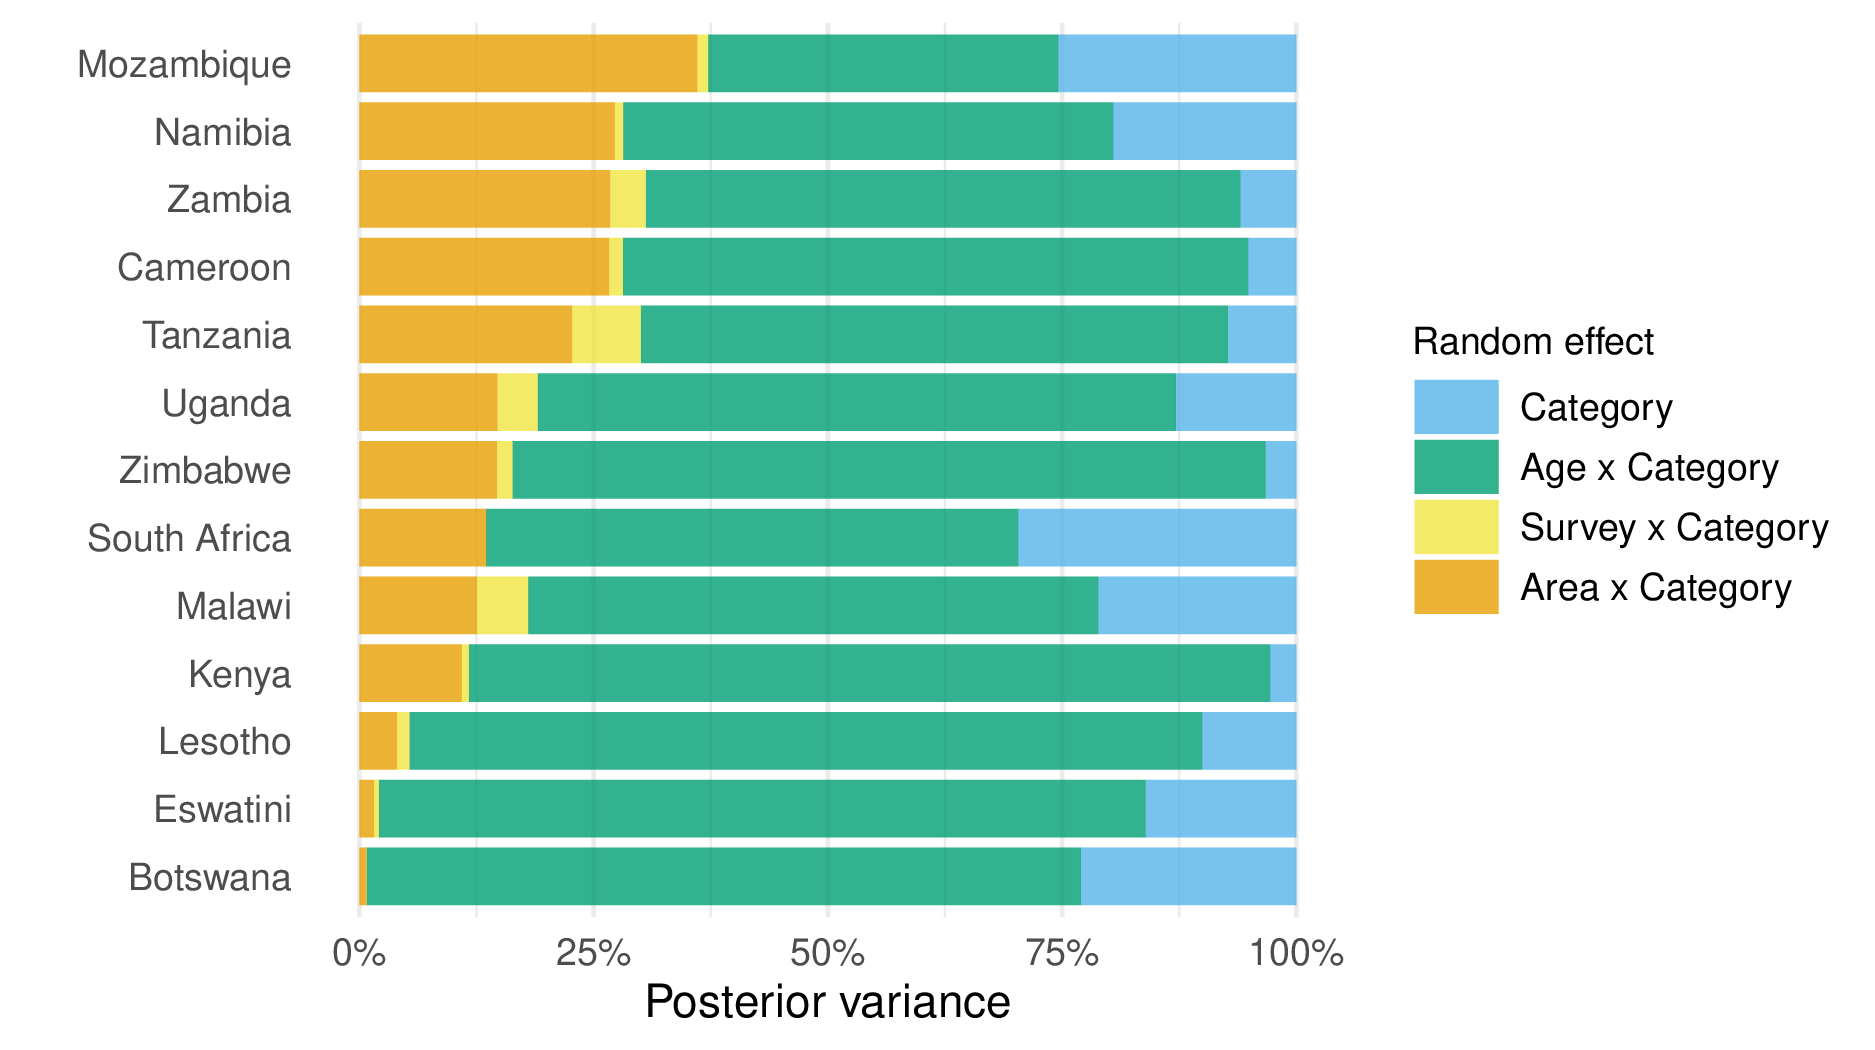
\includegraphics[width=0.95\linewidth]{resources/multi-agyw/20230627-144735-3da88508/depends/aaa-variance-proportions} 

}

\caption{Figure caption.}\label{fig:aaa-variance-proportions}
\end{figure}

Age group was the most important factor explaining variation in risk group proportions, accounting for 65.9\% (95\% CI 54.1--74.9\%) of total variation.
The primary change in risk group proportions by age group occurs between the 15-19 age group and 20-29 age group (Figure \ref{fig:3p1-continental-map}).
The next most important factor was location.
Country-level differences explained 20.9\% (95\% CI 11.9--34.5\%) of variation, while district-level variation within countries explained 11.3\% (95\% CI 8.2--15.3\%).
Temporal changes only explained 0.9\% (95\% CI 0.6--1.4\%) of variation, indicating very little change in risk group proportions over time.
I found similar variance decomposition results fitting each country individually (Figure \ref{fig:aaa-variance-proportions}) and using other model specifications.

\hypertarget{prevalence-and-incidence-by-risk-group}{%
\section{Prevalence and incidence by risk group}\label{prevalence-and-incidence-by-risk-group}}

Using the most recent risk group proportion estimates, I calculated the following indicators stratified according to district, age group and risk group:

\begin{enumerate}
\def\labelenumi{\arabic{enumi}.}
\tightlist
\item
  HIV prevalence \(\rho_{iak}\),
\item
  the number of people living with HIV (PLHIV) \(H_{iak}\),
\item
  HIV incidence \(\lambda_{iak}\), and
\item
  the number of new HIV infections \(I_{iak}\).
\end{enumerate}

To do so, I disaggregated district, age group specific Naomi estimates by risk group.

\hypertarget{disaggregation-of-naomi-prevalence-estimates}{%
\subsection{Disaggregation of Naomi prevalence estimates}\label{disaggregation-of-naomi-prevalence-estimates}}

To disaggregate HIV prevalence, I began by estimating HIV prevalence log odds ratios \(\log(\text{OR}_k)\) relative to the general population.
To do so, I fit a logistic regression model using age, country and risk group specific HIV prevalence bio-marker survey data.
I also included general population HIV prevalence data.
The logistic regression model included an indicator function for each risk group, and an indicator for being in the general population, such that the regression coefficients in this model correspond to log odds.
The log odds ratios may then be easily obtained by taking the difference in odds ratios.

To allow the log odds ratio for the highest risk group to vary based on general population prevalence I fit a linear regression of the FSW log odds against the general population log odds.
I ensured that log odds ratios for the FSW risk group were at least as large as those for the multiple or non-regular partner(s) risk group.

Given the fitted log odds ratios, I disaggregated Naomi estimates of PLHIV \(H_{ia}\) on the logit scale using numerical optimisation.
I did this by by finding the values of \(\theta_{ia}\) which minimise the equation
\begin{equation}
f(\theta_{ia}) = \sum_{k = 1}^4 \left( \text{logistic}(\theta_{ia} + \log(\text{OR}_k)) \cdot N_{iak} \right) - H_{ia},
\end{equation}
where
\begin{equation}
\text{logistic}(x) = \exp(x) / (1 + \exp(x)),
\end{equation}
such that
\begin{equation}
\text{logistic}(\hat \theta_{ia} + \log(\text{OR}_k)) = \rho_{iak}.
\end{equation}
These values are given by
\begin{equation}
\hat \theta_{ia} = \text{argmin}_{\theta_{ia} \in [-10, 10]} f(\theta_{ia})^2.
\end{equation}
The number of PLHIV were obtained by \(H_{iak} = \rho_{iak} N_{iak}\), where \(N_{iak}\) is the risk group population size.

\hypertarget{disaggregation-of-naomi-incidence-estimates}{%
\subsection{Disaggregation of Naomi incidence estimates}\label{disaggregation-of-naomi-incidence-estimates}}

I calculated the number of new HIV infections by risk group using linear disaggregation
\begin{align}
    I_{ia} &= \sum_k I_{iak} = \sum_k \lambda_{iak} (1 - \rho_{iak}) N_{iak} \\
    &= 0 + \lambda_{ia2} (1 - \rho_{ia2}) N_{ia2} + \lambda_{ia3} (1 - \rho_{ia3}) {ia3} + \lambda_{ia4} (1 - \rho_{ia4}) N_{ia4} \\
    &= \lambda_{ia2} \left((1 - \rho_{ia2}) N_{ia2}  + \text{RR}_{3} (1 - \rho_{ia3}) N_{ia3} + \text{RR}_4(\lambda_{ia}) (1 - \rho_{i4}) N_{ia4}  \right),
\end{align}
where \(\text{RR}_{2}\), \(\text{RR}_{3}\) and \(\text{RR}_{4}(\cdot)\) are the HIV risk ratios given in Table \ref{tab:risk-groups}, and \((1 - \rho_{iak}) N_{iak}\) are the susceptible population sizes in each risk group.
The risk ratio for FSW was defined as a function of district-level incidence in the general population \(\lambda_{ia}\).

Risk group specific HIV incidence estimates were then given by
\begin{align}
    \lambda_{ia1} &= 0, \\
    \lambda_{ia2} &= I_{ia} / \left((1 - \rho_{ia2}) N_{ia2} + \text{RR}_{3} (1 - \rho_{ia3}) N_{ia3} + \text{RR}_4(\lambda_{ia}) (1 - \rho_{ia4}) N_{ia4}\right), \\
    \lambda_{ia3} &= \text{RR}_{3} \lambda_{ia2}, \\
    \lambda_{ia4} &= \text{RR}_4(\lambda_{ia}) \lambda_{ia2}.
\end{align}
I evaluated these equations using Naomi model estimates of the number of new HIV infections \(I_{ia} = \lambda_{ia} N_{ia}\).
The number of new HIV infections were \(I_{iak} = \lambda_{iak} N_{iak}\).

\hypertarget{expected-new-infections-reached}{%
\subsection{Expected new infections reached}\label{expected-new-infections-reached}}

I calculated the number of new infections that would be reached prioritising according to each possible stratification of the population.
That is, for all \(2^3 = 8\) possible combinations of stratification by location, age, and risk group.

To illustrate this approach, consider stratification by age.
I first aggregated the number of new HIV infections and HIV incidence such that
\begin{align}
    I_a &= \sum_{ik} I_{iak}, \\
    \lambda_a &= I_a / \sum_{ik} (1 - \rho_{iak}) N_{iak}.
\end{align}
I then considered prioritisation individuals by age group \(a\) according to the highest HIV incidence \(\lambda_a\).
By cumulatively summing the expected infections, for each fraction of the total population reached I calculated the fraction of total expected new infections that would be reached.
As there are three age groups, the resulting function was piecewise linear with three segments.

\hypertarget{results-1}{%
\subsection{Results}\label{results-1}}



\begin{figure}

{\centering 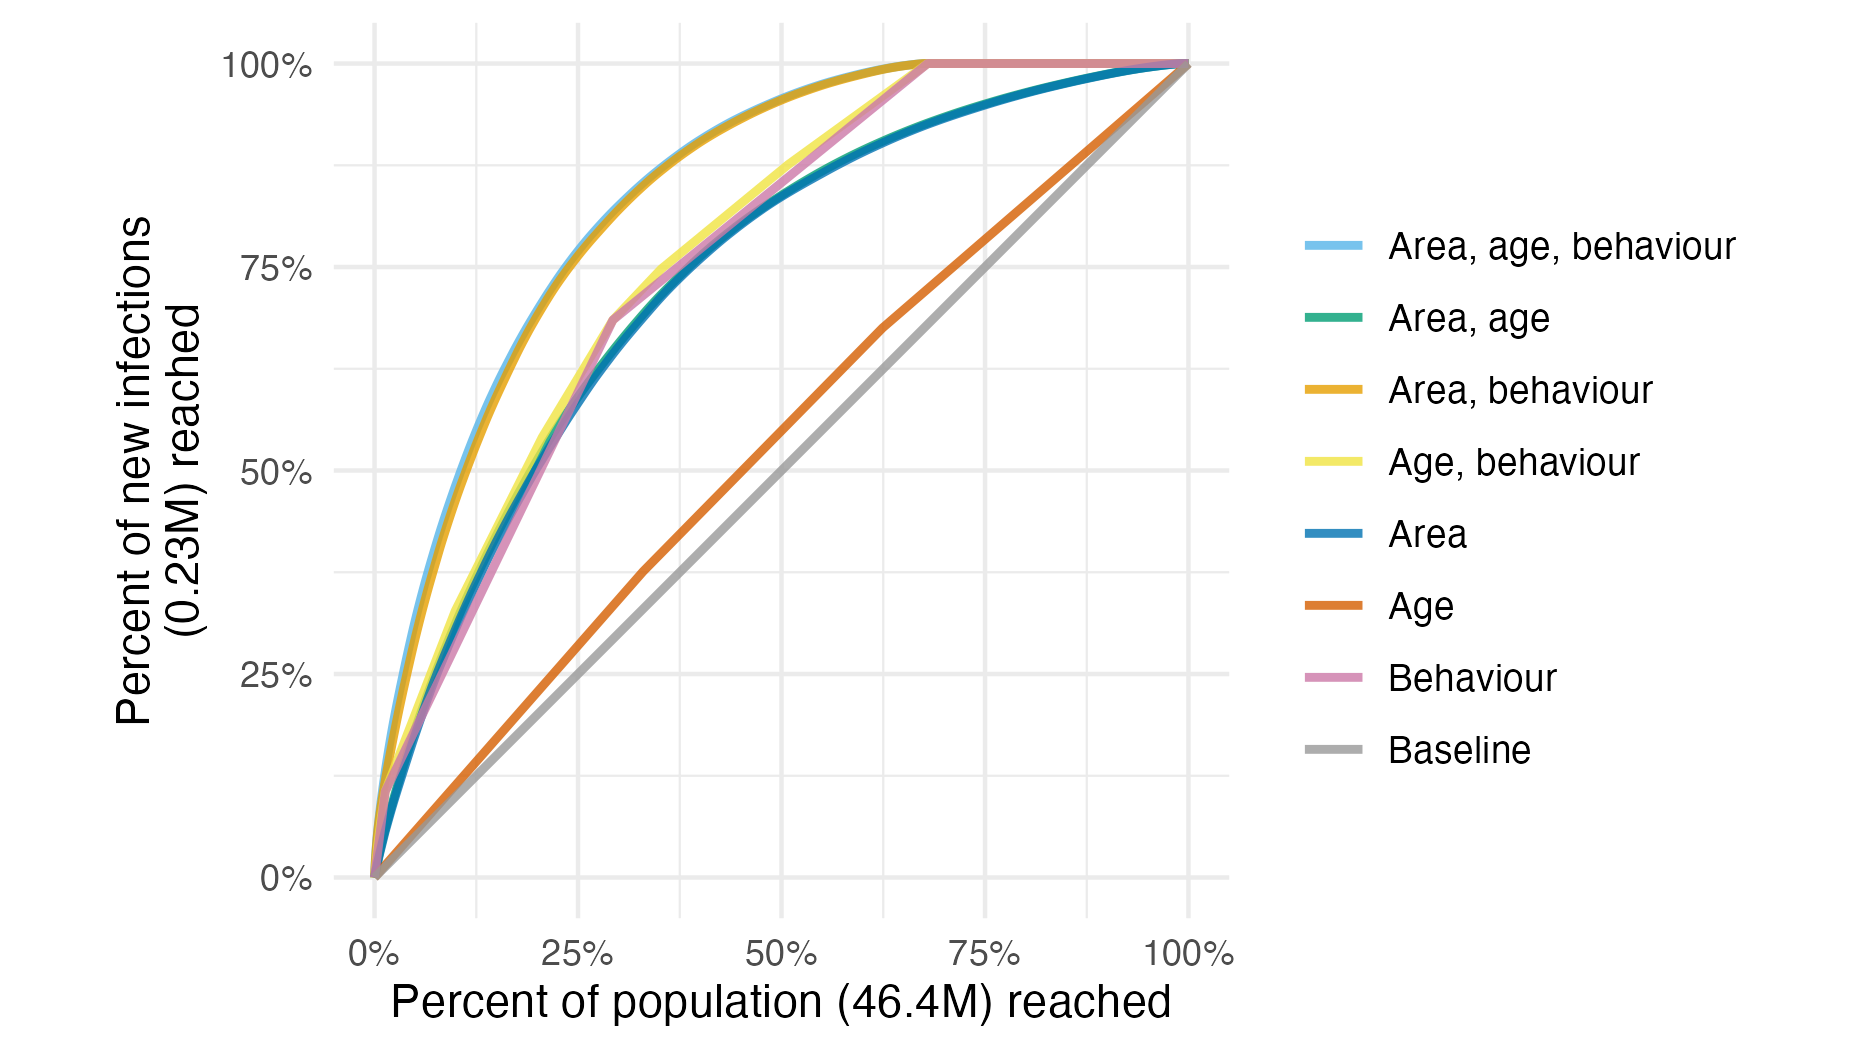
\includegraphics[width=0.95\linewidth]{resources/multi-agyw/20230627-144735-3da88508/depends/infections-reached} 

}

\caption{Percentage of new infections reached across all 13 countries, taking a variety of risk stratification approaches, against the percentage of at risk population required to be reached.}\label{fig:infections-reached}
\end{figure}

For any given fraction of AGYW prioritised, substantially more new infections were reached by strategies that included behavioural risk stratification.
Reaching half of all expected new infections required reaching 19.4\% of the population when stratifying by subnational area and age, but only 10.6\% when behavioural stratification was included (Figure \ref{fig:infections-reached}).
The majority of this benefit came from reaching FSW, who were 1.3\% of the population but 10.6\% of all new infections.

Considering each country separately, on average, reaching half of new infections in each country required reaching 14.6\% (range 8.7-21.8\%) of the population when stratifying by area and age, reducing to 5.1\% (range 2.1-13.2\%) when behaviour was included.
The relative importance of stratifying by age, location and behaviour varied between countries, analogous to the varying contribution of each to the total variance (Section \ref{variance-decomposition}).

\hypertarget{discussion-1}{%
\section{Discussion}\label{discussion-1}}

In this chapter, I estimated the proportion of AGYW who fall into different risk groups at a district level in 13 sub-Saharan African countries.
These estimates support consideration of differentiated prevention programming according to geographic locations and risk behaviour, as outlined in the Global AIDS Strategy.
Systematic differences in risk by age groups, and variation within and between countries, explained the large majority of variation in risk group proportions.
Changes over time were negligible in the overall variation in risk group proportions.
The proportion of 15-19 year olds who are sexually active, and among women aged 20-29 years, norms around cohabitation especially varied across districts and countries.
This variation underscores the need for these granular data to implement HIV prevention options aligned to local norms and risk behaviours.

I considered four risk groups based on sexual behaviour, the most proximal determinant of risk.
Other factors, such as condom usage or type of sexual act, may account for additional heterogeneity in risk from sexual behaviour.
However, I did not include these factors in view of measurement difficulties, concerns about consistency across contexts, and the operational benefits of describing risk parsimoniously.

Sexual behaviour confers risk only when AGYW reside in geographic locations where there is unsuppressed viral load among their potential partners.
I did not include more distal determinants, such as school attendance, orphanhood, or gender empowerment, as I expect their effects on risk to largely be mediated by more proximal determinants.
However, to effectively implement programming, it is crucial to understand these factors, as well as the broader structural barriers and limits to personal agency faced by AGYW.
Importantly, programs must ensure that intervention prioritisation occurs without stigmatising or blaming AGYW.

By considering a range of possible risk stratification strategies, I showed that successful implementation of a risk-stratified approach would allow substantially more of those at risk for infections to be identified before infection occurs.
A considerable proportion of estimated new infections were among FSW, supporting the case for HIV programming efforts focused on key population groups \autocite{baral2012burden}.
There is substantial variation in the importance of prioritisation by age, location and behaviour within each country.
This highlights the importance of understanding and tailoring HIV prevention efforts to country-specific contexts.
By standardising the analysis across all 13 countries, I showed the additional efficiency benefits of resource allocation between countries.

I found a geographic delineation in the proportion of women cohabiting between southern and eastern Africa, calling attention to a divide attributable to many cultural, social, and economic factors.
The delineation does not represent a boundary between predominately Christian and Muslim populations, which is further north.
I also note that the high numbers of adolescent girls aged 15-19 cohabiting in Mozambique is markedly different from the other countries \autocite{unicef}.

\textcite{brugh2021characterizing} previously geographically mapped AGYW HIV risk groups using biomarker and behavioural data from the most recent surveys in Eswatini, Haiti and Mozambique to define and subsequently map risk groups with a range of machine learning techniques.
My work builds on \textcite{brugh2021characterizing} by including more countries, integrating a greater number of surveys, and connecting risk group proportions with HIV epidemic indicators to help inform programming.

My modelled estimates of risk group proportions improve upon direct survey results for three reasons.
First, by taking a modular modelling approach, I integrated all relevant survey information from multiple years, allowing estimation of the FSW proportion for surveys without a specific transactional sex question.
Second, whereas direct estimates exhibit large sampling variability at a district level, I alleviated this issue using spatio-temporal smoothing (Figure \ref{fig:model-direct-benefits}).
Third, I provided estimates in all district-years, including those not directly sampled by surveys, allowing estimates to be consistently fed into further analysis and planning pipelines such as my analysis of risk group specific prevalence and incidence (Figure \ref{fig:model-direct-benefits}).



\begin{figure}

{\centering 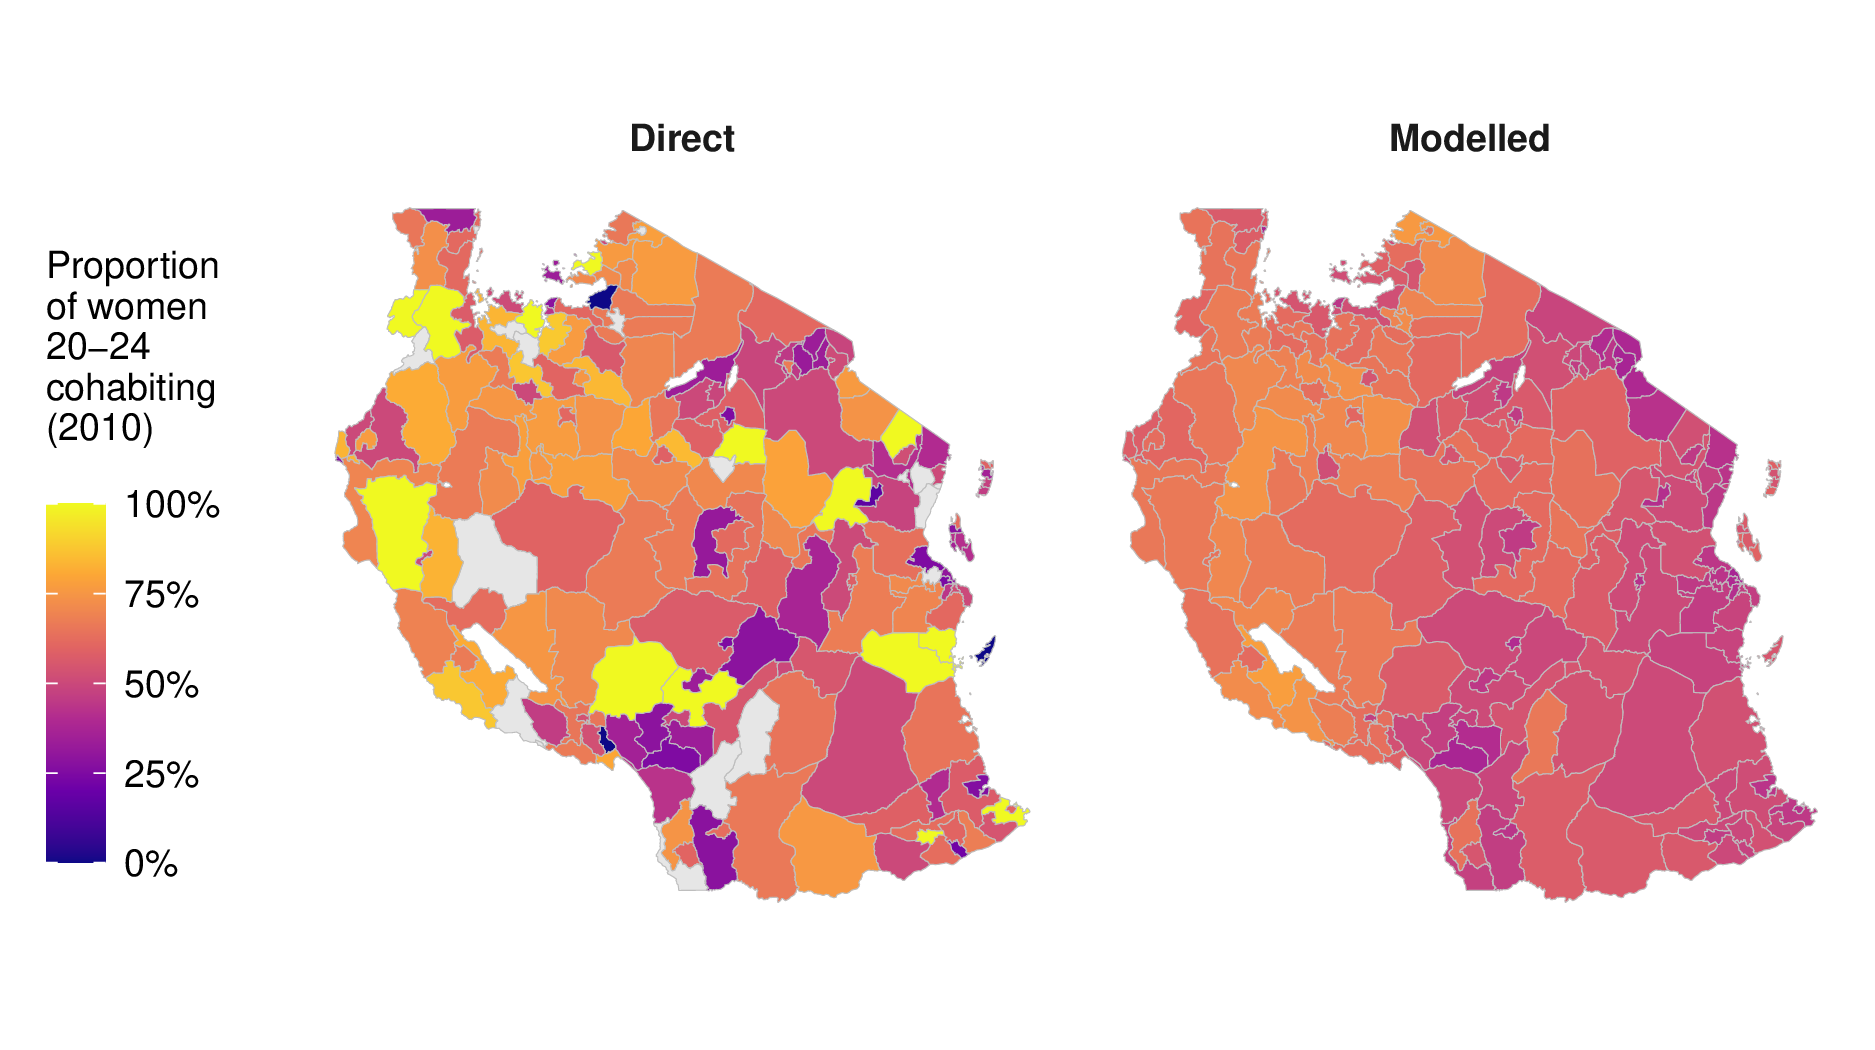
\includegraphics[width=0.95\linewidth]{resources/multi-agyw/20230627-144735-3da88508/depends/model-direct-benefits} 

}

\caption{Figure caption.}\label{fig:model-direct-benefits}
\end{figure}

The final surveys included in the risk model model were conducted in 2018.
The analysis may be updated with more surveys as they become available.
I do not anticipate that the risk group proportions will change substantially, as I found that they did not change significantly over time.

My analysis focused on females aged 15-29 years, and could be extended to consider optimisation of prevention more broadly, accounting for the 0\% of new infections among adults 15-49 which occur in women 30-49 and men 15-49.
Estimating sexual risk behaviour in adults 15-49 would be a crucial step toward greater understanding of the dynamics of the HIV epidemic in sub-Saharan Africa, and would allow incidence models to include stratification of individuals by sexual risk.

\hypertarget{limitations}{%
\subsection{Limitations}\label{limitations}}

This analysis was subject to challenges shared by most approaches to monitoring sexual behaviour in the general population \autocite{cleland2004monitoring}.
In particular, under-reporting of higher risk sexual behaviours among AGYW could affect the validity of my risk group proportion estimates.
Due to social stigma or disapproval, respondents may be reluctant to report non-marital partners \autocite{nnko2004secretive,helleringer2011reliability} or may bias their reporting of sexual debut \autocite{zaba2004age,wringe2009comparative,nguyen2022trends}.
For guidance of resource allocation, differing rates of under-reporting by country, district, year or age group are particularly concerning to the applicability of my results; and, while it may be reasonable to assume a constant rate over space-time, the same cannot be said for age, where aspects of under-reporting have been shown to decline as respondents age \autocite{glynn2011assessing}, suggesting that the elevated risks I found faced by younger women are likely a conservative estimate.
If present, these reporting biases will also have distorted the estimates of infection risk ratios and prevalence ratios I used in my analysis, likely over-attributing risk to higher risk groups.

I have the least confidence in my estimates for the FSW risk group.
As well as having the smallest sample sizes, my transactional sex estimates do not overcome the difficulties of sampling hard to reach groups.
I inherent any limitations of the national FSW estimates \autocite{stevens2022estimating} which I adjust my estimates of transactional sex to match.
Furthermore, I do not consider seasonal migration patterns, which may particularly affect FSW population size.
More generally, I did not consider covariates potentially predictive of risk group proportions (such as sociodemographic characteristics, education, local economic activity, cultural and religious norms and attitudes), which are typically difficult to measure spatially.
Identifying measurable correlates of risk, or particular settings in which time-concentrated HIV risk occurs, is an important area for further research to improve risk prioritisation and precision HIV programme delivery.

The efficiency of each stratified prevention strategy depends on the ability of programmes to identify and effectively reach those in each strata.
My analysis of new infections potentially averted assumed a ``best-case'' scenario where AGYW of every strata can be reached perfectly, and should therefore be interpreted as illustrating the potentially obtainable benefits rather than benefits which would be obtained from any specific intervention strategy.
In practice, stratified prevention strategies are likely to be substantially less efficient than this best-case scenario.
Factors I did not consider include the greater administrative burden of more complex strategies, variation in difficulty or feasibility of reaching individuals in each strata, variation in the range or effectiveness of interventions by strata, and changes in strata membership that may occur during the course of a year.
Identifying and reaching behavioural strata may be particularly challenging.
Empirical evaluations of behavioural risk screening tools have found only moderate discriminatory ability \autocite{jia2022risk}, and risk behaviour may change rapidly among young populations, increasing the challenge to effectively deliver appropriately timed prevention packages.
This consideration may motivate selecting risk groups based on easily observable attributes, such as attendance of a particular service or facility, rather than sexual behaviour.

In conducting this work, there was insufficient engagement with country experts or civil society organisations.
As a result, in early use of the risk group tool the FSW population size estimates were met with some disagreement in Malawi.
In that instance, the cause of the disagreement was extenal model inputs used.
In future, estimates should be generated and reviewed by country teams.

\hypertarget{conclusion}{%
\subsection{Conclusion}\label{conclusion}}

I estimated HIV risk group proportions, HIV prevalences and HIV incidences for AGYW aged 15-19, 20-24 and 25-29 years at a district-level in 13 priority countries.
Using these estimates, I analysed the number of infections that could be reached by prioritisation based upon location, age and behaviour.
Though subject to limitations, these estimates provide data that national HIV programmes can use to set targets and implement differentiated HIV prevention strategies as outlined in the Global AIDS Strategy.
Successfully implementing this approach would result in more efficiently reaching a greater number of those at risk of infection.

Among AGYW, there was systematic variation in sexual behaviour by age and location, but not over time.
Age group variation was primarily attributable to age of sexual debut (ages 15-24).
Spatial variation was particularly present between those who reported one cohabiting partner versus non-regular or multiple partners.
Risk group proportions did not change substantially over time, indicating that norms relating to sexual behaviour are relatively static.
These findings underscore the importance of providing effective HIV prevention options tailored to the needs of particular age groups, as well as local norms around sexual partnerships.

\hypertarget{naomi-aghq}{%
\chapter{Fast approximate Bayesian inference}\label{naomi-aghq}}

\adjustmtc
\markboth{Fast approximate Bayesian inference}{}

This chapter describes a novel Bayesian inference method.
Development of the method was motivated the Naomi small-area estimation model.
Over 35 countries have used the Naomi model software (\href{https://naomi.unaids.org}{\texttt{https://naomi.unaids.org}}) to produce subnational estimates of HIV indicators \autocite{unaids2023global}.
The complexity of the model makes obtaining the fast and accurate Bayesian inferences required in this setting challenging.
As such, inferences have previously been obtained using an empirical Bayes approximation to full Bayesian inference.
This is undesirable as it leads to underestimating the uncertainty in key HIV indicators, and ultimately worse policy.

The methods developed in this chapter combine Laplace approximations with adaptive quadrature, and descend from the integrated nested Laplace approximation of \textcite{rue2009approximate}.
I implement an INLA-like algorithm using automatic differentiation, and enable the use of this algorithm for a wider class of models than previously possible.

I began work on this project at the start of my PhD, and only began making meaningful progress after reading \textcite{stringer2022fast}.
I am grateful to later have had the opportunity to collaborate with Alex Stringer, including visiting the University of Waterloo in fall term of 2022.
The results of this work are presented in \textcite{howes2023fast}.
Code for the analysis in this chapter is available from \href{https://github.com/athowes/elgm-inf}{\texttt{https://github.com/athowes/naomi-aghq}}.

\hypertarget{inference-methods}{%
\section{Inference methods}\label{inference-methods}}

In a Bayesian analysis, the primary goal is to perform inference.
That is, to obtain the posterior distribution
\begin{equation}
p(\boldsymbol{\mathbf{\phi}} \, | \, \mathbf{y}) = \frac{p(\boldsymbol{\mathbf{\phi}}, \mathbf{y})}{p(\mathbf{y})},
\end{equation}
or some way to compute relevant functions of it.
As usual, \(\boldsymbol{\mathbf{\phi}} = (\phi_1, \ldots, \phi_d)\) are the parameters and \(\mathbf{y} = (y_1, \ldots, y_n)\) are the data.

Inference is a sensible goal because the posterior distribution is sufficient for use in decision making.
Given a loss function \(l(a, \boldsymbol{\mathbf{\phi}})\) the expected posterior loss of a decision \(a\) depends on the data only via the posterior distribution
\begin{equation}
\mathbb{E}(l(a, \boldsymbol{\mathbf{\phi}}) \, | \, \mathbf{y}) = \int_{\mathbb{R}^d} l(a, \boldsymbol{\mathbf{\phi}}) p(\boldsymbol{\mathbf{\phi}} \, | \, \mathbf{y}) \text{d}\boldsymbol{\mathbf{\phi}}.
\end{equation}
For example, given the posterior distribution of the current demand for HIV treatment at a particular facility, historic data about treatment demand are not required for planning of service provision.

It is usually intractable to straightforwardly obtain the posterior distribution.
This is because the denominator contains a potentially high-dimensional integral over the parameters
\begin{equation}
p(\mathbf{y}) = \int_{\mathbb{R}^d} p(\mathbf{y}, \boldsymbol{\mathbf{\phi}}) \text{d}\boldsymbol{\mathbf{\phi}}, \label{eq:evidence}
\end{equation}
sometimes called the evidence or posterior normalising constant.
For this reason, approximations to the posterior distribution \(\tilde p(\boldsymbol{\mathbf{\phi}} \, | \, \mathbf{y})\) are typically used in place of the exact posterior distribution.

Some approximate Bayesian inference methods avoid directly calculating the posterior normalising constant, instead working with the unnormalised posterior distribution
\begin{equation}
p(\boldsymbol{\mathbf{\phi}} \, | \, \mathbf{y}) \propto p(\boldsymbol{\mathbf{\phi}}, \mathbf{y}).
\end{equation}
Other approximate Bayesian inference methods can more directly be thought of as ways to estimate the posterior normalising constant.
The methods in this chapter fall into this later category.

\hypertarget{the-laplace-approximation}{%
\subsection{The Laplace approximation}\label{the-laplace-approximation}}

Laplace's method \autocite{laplace1774memoire} is a technique used to approximate integrals of the form
\begin{equation}
\int \exp(C h(\mathbf{z})) \text{d}\mathbf{z},
\end{equation}
where \(C > 0\) is a large constant and \(h\) is a function which is twice-differentiable, and \(\mathbf{z}\) are generic variables.
The Laplace approximation \autocite{tierney1986accurate} is obtained by application of Laplace's method to calculate the posterior normalising constant.
Let \(h(\boldsymbol{\mathbf{\phi}}) = \log p(\boldsymbol{\mathbf{\phi}}, \mathbf{y})\) such that
\begin{equation}
p(\mathbf{y}) = \int_{\mathbb{R}^d} p(\mathbf{y}, \boldsymbol{\mathbf{\phi}}) \text{d}\boldsymbol{\mathbf{\phi}} = \int_{\mathbb{R}^d} \exp(h(\boldsymbol{\mathbf{\phi}})) \text{d}\boldsymbol{\mathbf{\phi}}.
\end{equation}
Laplace's method involves approximating the function \(h\) by its second order Taylor expansion.
This expansion is then evaluated at a maxima of \(h\) to eliminate the first order term.
Let
\begin{equation}
\hat{\boldsymbol{\mathbf{\phi}}} = \arg\max_{\boldsymbol{\mathbf{\phi}}} h(\boldsymbol{\mathbf{\phi}}) \label{eq:posterior-mode}
\end{equation}
be the posterior mode, and
\begin{equation}
\hat {\mathbf{H}} = - \frac{\partial^2}{\partial \boldsymbol{\mathbf{\phi}} \partial \boldsymbol{\mathbf{\phi}}^\top} h(\boldsymbol{\mathbf{\phi}}) \rvert_{\boldsymbol{\mathbf{\phi}} = \hat{\boldsymbol{\mathbf{\phi}}}} \label{eq:hessian}
\end{equation}
be the Hessian matrix evaluated at the posterior mode.
The Laplace approximation is then
\begin{align}
\tilde p_{\texttt{LA}}(\mathbf{y}) &= \int_{\mathbb{R}^d} \exp \left( h(\hat{\boldsymbol{\mathbf{\phi}}}) - \frac{1}{2} (\boldsymbol{\mathbf{\phi}} - \hat{\boldsymbol{\mathbf{\phi}}})^\top \hat {\mathbf{H}} (\boldsymbol{\mathbf{\phi}} - \hat{\boldsymbol{\mathbf{\phi}}}) \right) \text{d}\boldsymbol{\mathbf{\phi}} \label{eq:la} \\
&= p(\hat{\boldsymbol{\mathbf{\phi}}}, \mathbf{y}) \cdot \frac{(2 \pi)^{d/2}}{| \hat {\mathbf{H}} |^{1/2}}. \label{eq:la2}
\end{align}
The result above is calculated using the known normalising constant of the Gaussian distribution
\begin{equation}
p_\texttt{G}(\boldsymbol{\mathbf{\phi}} \, | \, \mathbf{y}) = \mathcal{N}(\boldsymbol{\mathbf{\phi}} \, | \, \hat{\boldsymbol{\mathbf{\phi}}}, \hat {\mathbf{H}}^{-1}) = \frac{| \hat {\mathbf{H}} |^{1/2}}{(2 \pi)^{d/2}} \exp \left( - \frac{1}{2} (\boldsymbol{\mathbf{\phi}} - \hat{\boldsymbol{\mathbf{\phi}}})^\top \hat {\mathbf{H}} (\boldsymbol{\mathbf{\phi}} - \hat{\boldsymbol{\mathbf{\phi}}}) \right).
\end{equation}
The Laplace approximation may be thought of as approximating the posterior distribution by a Gaussian distribution \(p(\boldsymbol{\mathbf{\phi}} \, | \, \mathbf{y}) \approx p_\texttt{G}(\boldsymbol{\mathbf{\phi}} \, | \, \mathbf{y})\) such that
\begin{equation}
\tilde p_{\texttt{LA}}(\mathbf{y}) = \frac{p(\boldsymbol{\mathbf{\phi}}, \mathbf{y})}{p_\texttt{G}(\boldsymbol{\mathbf{\phi}} \, | \, \mathbf{y})} \Big\rvert_{\boldsymbol{\mathbf{\phi}} = \hat{\boldsymbol{\mathbf{\phi}}}}.
\end{equation}

Calculation of the Laplace approximation requires obtaining the second derivative of \(h\) with respect to \(\boldsymbol{\mathbf{\phi}}\) (Equation \eqref{eq:hessian}).
The performance of the optimisation algorithm used to obtain the maxima of \(h\) (Equation \eqref{eq:posterior-mode}) may be improved by providing access to the gradient of \(h\) with respect to \(\boldsymbol{\mathbf{\phi}}\).



\begin{figure}

{\centering 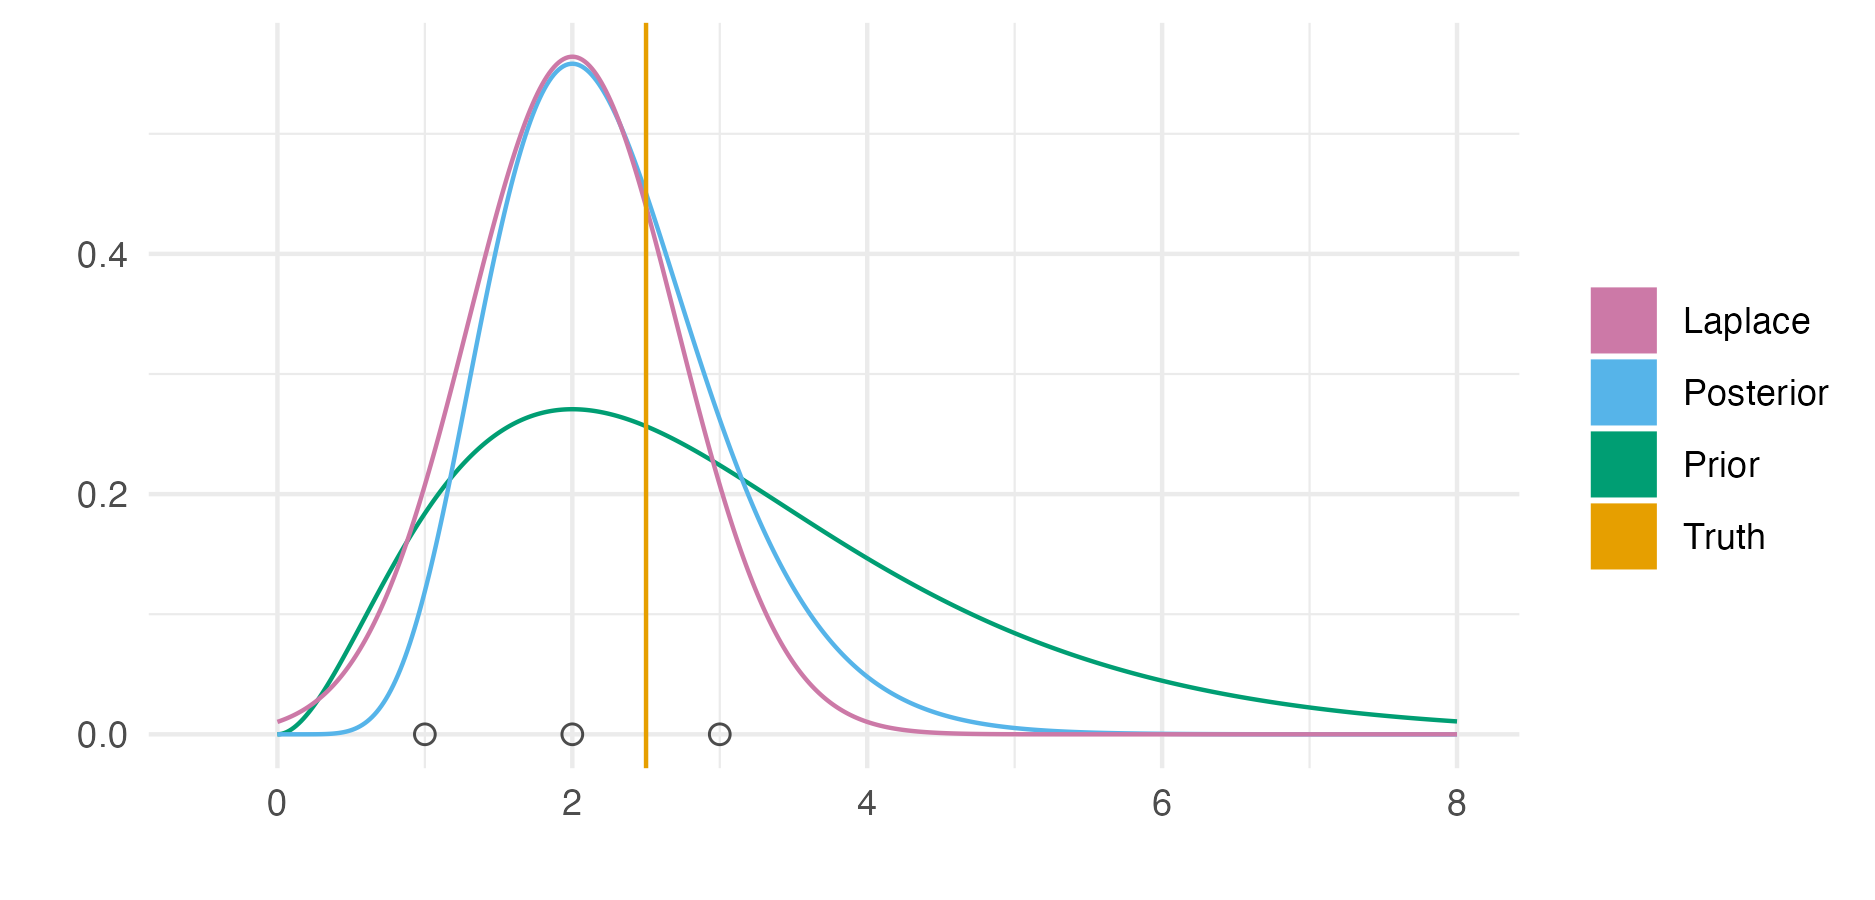
\includegraphics[width=0.95\linewidth]{figures/naomi-aghq/laplace} 

}

\caption{Demonstration of the Laplace approximation for the simple Bayesian inference example of Figure \ref{fig:conjugate}. The unnormalised posterior is \(p(\phi, \mathbf{y}) = \phi^8 \exp(-4 \phi)\), and can be recognised as the unnomalised gamma distribution \(\text{Gamma}(9, 4)\). The true log normalising constant is \(\log p(\mathbf{y}) = \log\Gamma(9) - 9 \log(4) = -1.872046\), whereas the Laplace approximate log normalising constant is \(\log \tilde p_{\texttt{LA}}(\mathbf{y}) = -1.882458\), resulting from the Gaussian approximation \(p_\texttt{G}(\phi \, | \, \mathbf{y}) = \mathcal{N}(\phi \, | \,\mu = 2, \tau = 2)\).}\label{fig:laplace}
\end{figure}

\hypertarget{marginal-la}{%
\subsubsection{The marginal Laplace approximation}\label{marginal-la}}

Approximating the full joint posterior distribution using a Gaussian distribution may be inaccurate.
An alternative is to approximate the marginal posterior distribution of some subset of the parameters which might have posterior distributions which are close to being Gaussian.

Let \(\boldsymbol{\mathbf{\phi}} = (\mathbf{x}, \boldsymbol{\mathbf{\theta}})\) and consider a three-stage hierarchical model
\begin{equation}
p(\mathbf{y}, \mathbf{x}, \boldsymbol{\mathbf{\theta}}) = p(\mathbf{y} \, | \, \mathbf{x}, \boldsymbol{\mathbf{\theta}}) p(\mathbf{x} \, | \, \boldsymbol{\mathbf{\theta}}) p(\boldsymbol{\mathbf{\theta}}),
\end{equation}
where \(\mathbf{x}\) is the latent field, and \(\boldsymbol{\mathbf{\theta}}\) are the hyperparameters.
Applying an equivalent Laplace approximation to the latent field, we have \(h(\mathbf{x}, \boldsymbol{\mathbf{\theta}}) = \log p(\mathbf{y}, \mathbf{x}, \boldsymbol{\mathbf{\theta}})\) with posterior mode
\begin{equation}
\hat{\mathbf{x}}(\boldsymbol{\mathbf{\theta}}) = \arg\max_{\mathbf{x}} h(\mathbf{x}, \boldsymbol{\mathbf{\theta}}) \label{eq:marginal-posterior-mode}
\end{equation}
and Hessian matrix evaluated at the posterior mode
\begin{equation}
\hat {\mathbf{H}}(\boldsymbol{\mathbf{\theta}}) = - \frac{\partial^2}{\partial \mathbf{x} \partial \mathbf{x}^\top} h(\mathbf{x}, \boldsymbol{\mathbf{\theta}}) \rvert_{\mathbf{x} = \hat{\mathbf{x}}(\boldsymbol{\mathbf{\theta}})}. \label{eq:marginal-hessian}
\end{equation}
In both Equation \eqref{eq:marginal-posterior-mode} and \eqref{eq:marginal-hessian} dependence on the hyperparameters \(\boldsymbol{\mathbf{\theta}}\) is made explicit.
The resulting marginal Laplace approximation is then
\begin{align}
\tilde p_{\texttt{LA}}(\boldsymbol{\mathbf{\theta}}, \mathbf{y}) &= \int_{\mathbb{R}^N} \exp \left( h(\hat{\mathbf{x}}(\boldsymbol{\mathbf{\theta}}), \boldsymbol{\mathbf{\theta}}) - \frac{1}{2} (\mathbf{x} - \hat{\mathbf{x}}(\boldsymbol{\mathbf{\theta}}))^\top \hat {\mathbf{H}}(\boldsymbol{\mathbf{\theta}}) (\mathbf{x} - \hat{\mathbf{x}}(\boldsymbol{\mathbf{\theta}})) \right) \text{d}\mathbf{x} \label{eq:marginalla} \\
&= \exp(h(\hat{\mathbf{x}}(\boldsymbol{\mathbf{\theta}}), \mathbf{y})) \cdot \frac{(2 \pi)^{d/2}}{| \hat {\mathbf{H}}(\boldsymbol{\mathbf{\theta}}) |^{1/2}} \\
&= \frac{p(\mathbf{y}, \mathbf{x}, \boldsymbol{\mathbf{\theta}})}{\tilde p_\texttt{G}(\mathbf{x} \, | \, \boldsymbol{\mathbf{\theta}}, \mathbf{y})} \Big\rvert_{\mathbf{x} = \hat{\mathbf{x}}(\boldsymbol{\mathbf{\theta}})},
\end{align}
where \(\tilde p_\texttt{G}(\mathbf{x} \, | \, \boldsymbol{\mathbf{\theta}}, \mathbf{y}) = \mathcal{N}(\mathbf{x} \, | \, \hat{\mathbf{x}}(\boldsymbol{\mathbf{\theta}}), \hat{\mathbf{H}}(\boldsymbol{\mathbf{\theta}})^{-1})\) is a Gaussian approximation to the marginal posterior of the latent field.

The marginal Laplace approximation is most accurate when then marginal posterior \(p(\mathbf{x} \, | \, \boldsymbol{\mathbf{\theta}}, \mathbf{y})\) is accurately approximated by a Gaussian
distribution.
For the class of latent Gaussian models \autocite{rue2009approximate} the prior on the latent field is Gaussian \(\mathbf{x} \sim \mathcal{N}(\mathbf{x} \, | \, \boldsymbol{\mathbf{\theta}})\).
The marginal posterior is then given by\ldots{}

\hypertarget{quadrature}{%
\subsection{Quadrature}\label{quadrature}}

Quadrature is an method used to approximate integrals with a weighted sum of function evaluations.
As with the Laplace approximation, it is deterministic in that the computational procedure is not intrinsically random.
Let \(\mathcal{Q}\) be a set of quadrature nodes \(\mathbf{z} \in \mathcal{Q}\) and \(\omega: \mathbb{R}^d \to \mathbb{R}\) be a weighting function.
Then, quadrature can be used to estimate the posterior normalising constant by
\begin{equation}
\tilde p_{\mathcal{Q}}(\mathbf{y}) = \sum_{\mathbf{z} \in \mathcal{Q}} p(\mathbf{y}, \mathbf{z}) \omega(\mathbf{z}).
\end{equation}

To illustrate how quadrature works for a simple example, consider integrating the univariate function \(f(z) = z \sin(z)\) between \(z = 0\) and \(z = \pi\).
A quadrature approximation of this integral is
\begin{equation}
\int_{0}^\pi z \sin(z) \text{d} z \approx \sum_{z \in \mathcal{Q}} z \sin(z) \omega(z),
\end{equation}
where \(\mathcal{Q} = \{z_1, \ldots z_k\}\) are a set of \(k\) quadrature nodes and \(\omega: \mathbb{R} \to \mathbb{R}\).

The trapezoid rule is an example of a quadrature rule, where \(z_i - z_{i - 1} = \epsilon_i > 0\) for all \(1 < i < k\), and \(\omega(z_i) = \epsilon\) for \(1 < i < k\) and \(\omega(z_i) = \epsilon / 2\) for \(i \in \{1, k\}\).
Figure \ref{fig:trapezoid} shows in application of the trapezoid rule, the more quadrature nodes are used, the more accurate the estimate of the integrand is.
Under some regularity conditions on \(f\), as \(\epsilon \to 0\) the quadrature estimate obtained using the trapezoid rule converges to the true value of the integral.
Indeed, this approach was used by Riemann to provide the first rigorous definition of the integral.



\begin{figure}

{\centering 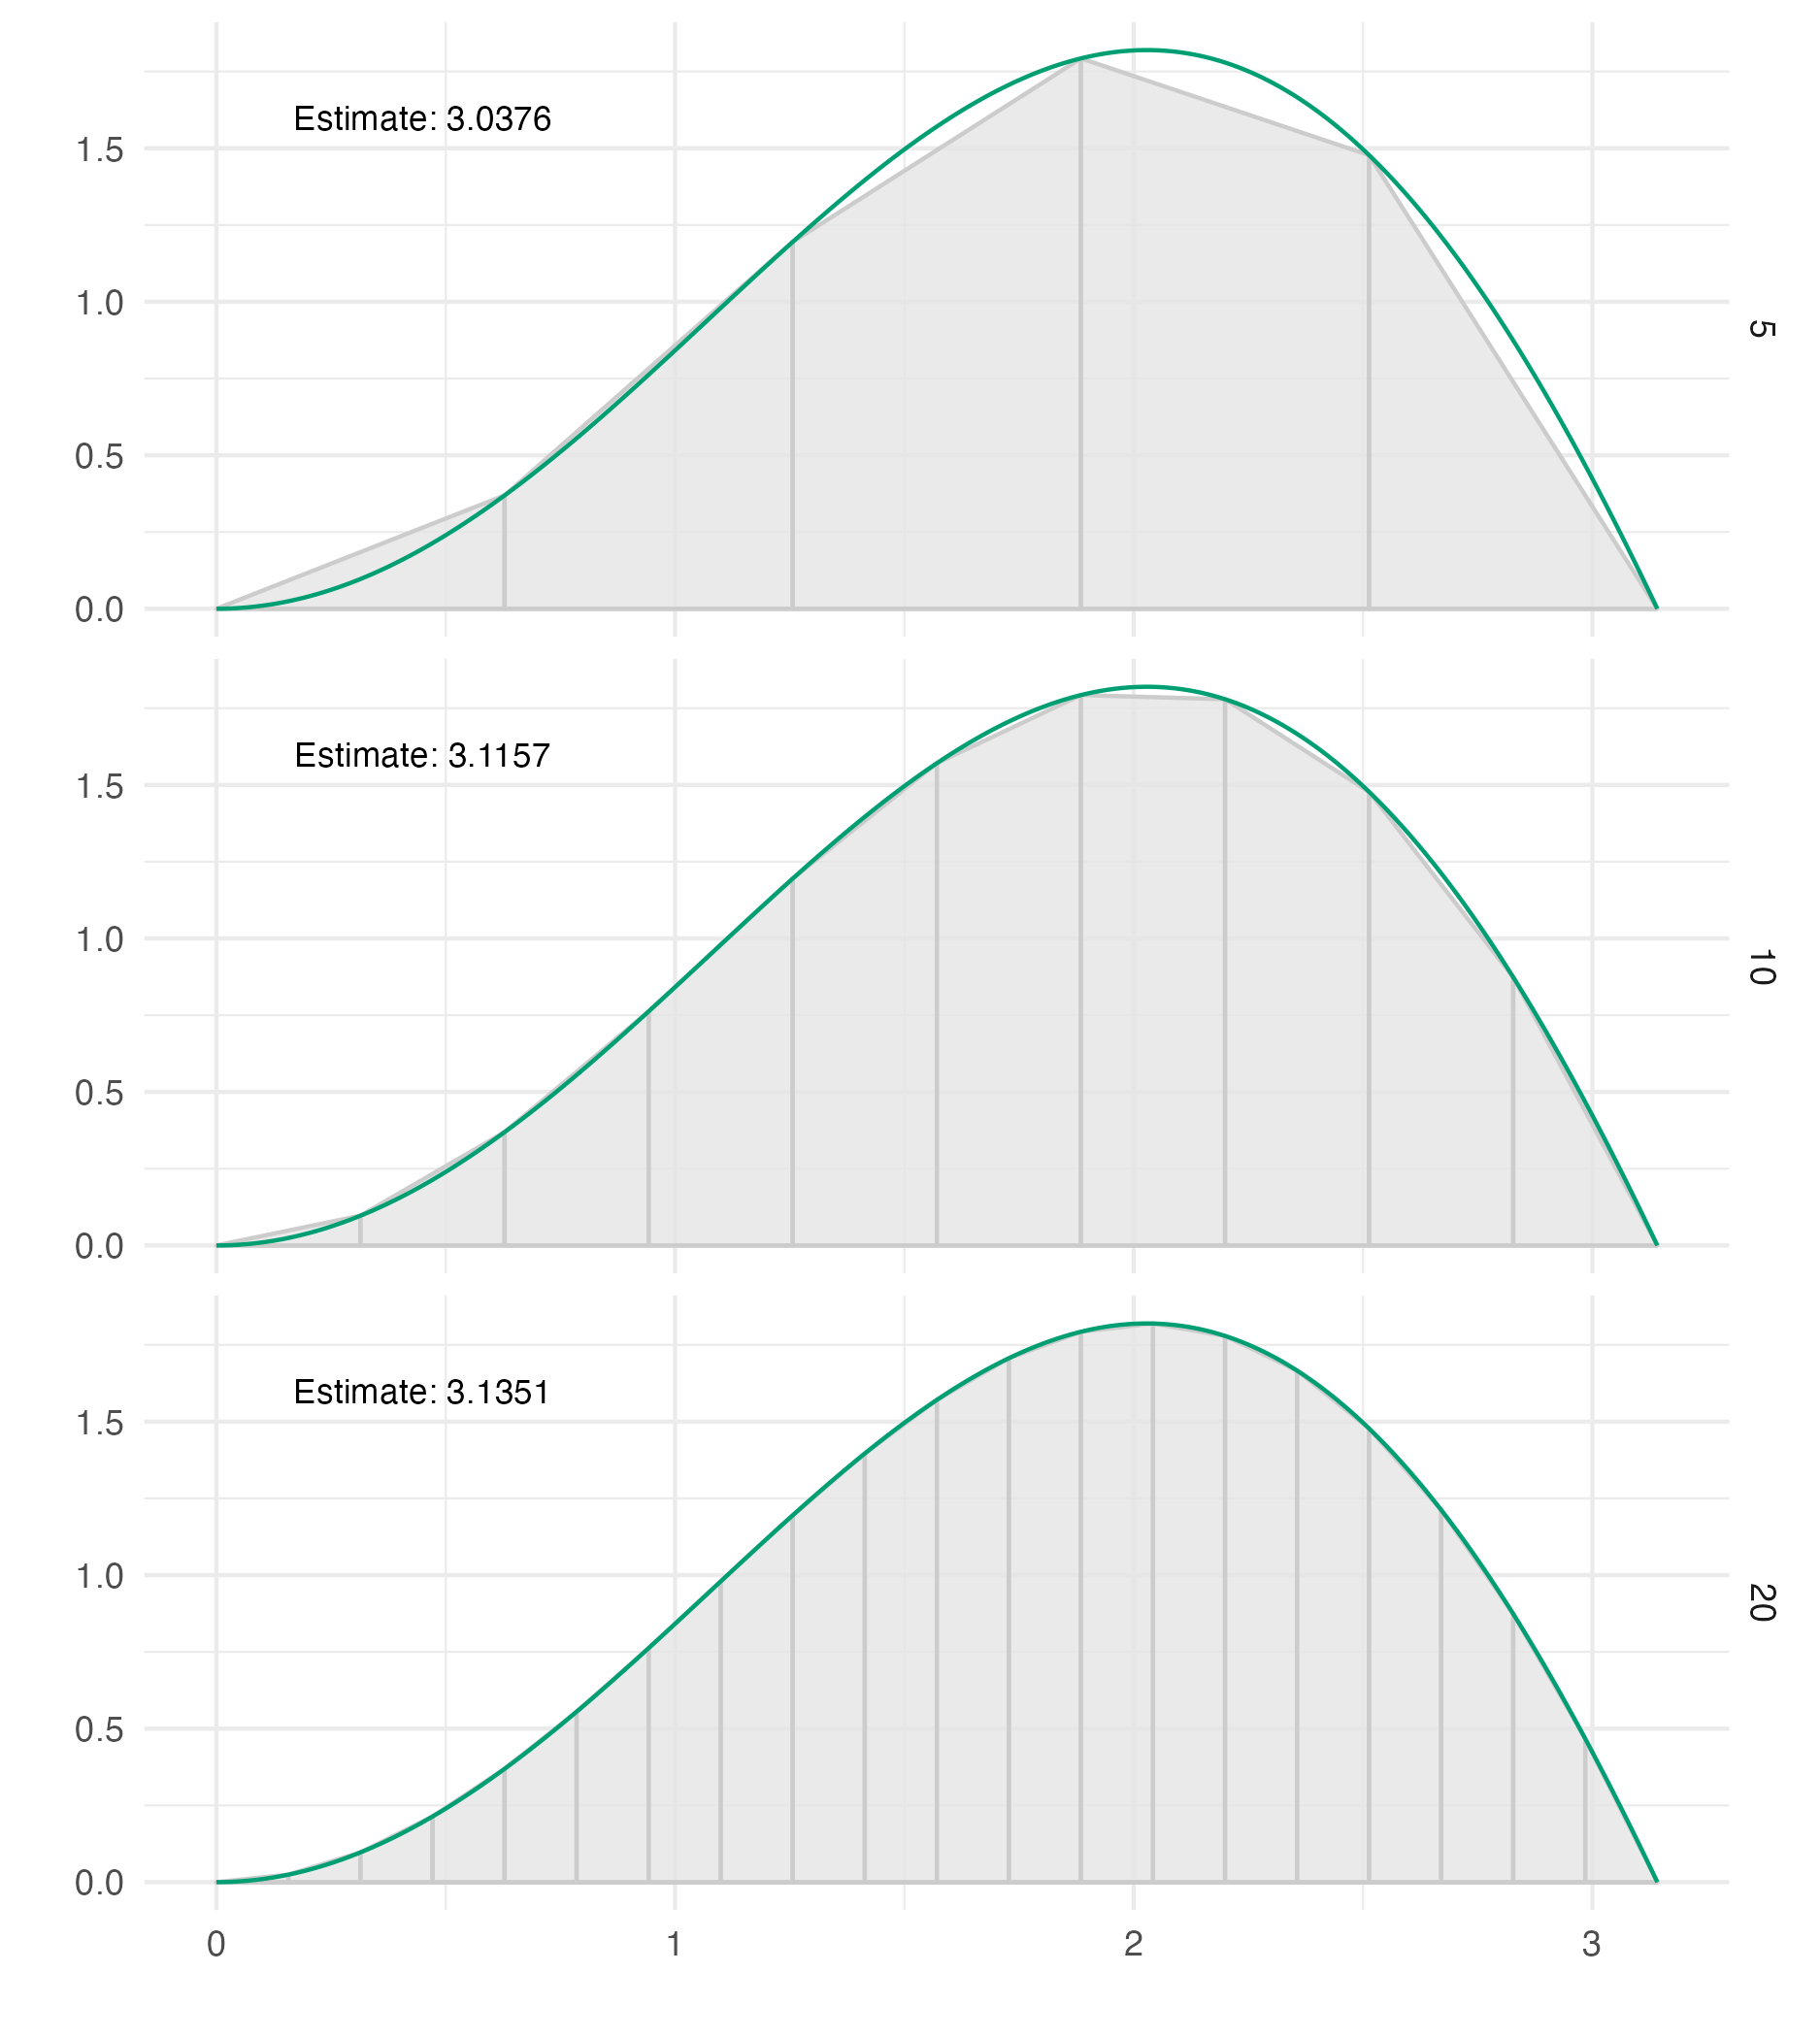
\includegraphics[width=0.95\linewidth]{figures/naomi-aghq/trapezoid} 

}

\caption{The trapezoid rule with \(k = 5, 25, 125\) equally-spaced (\(\epsilon_i = \epsilon\)) quadrature nodes can be used to integrate the function \(f(z) = z \sin(z)\) in the domain \([0, \pi]\). Here, the exact solution is \(\pi \approx 3.1416\). As \(k\) increases and more nodes are used in the computation, the quadrature estimate becomes closer to the exact solution.}\label{fig:trapezoid}
\end{figure}

Quadrature methods are most effective when integrating over small dimensions.
This is because the number of quadrature nodes required to be evaluated in the computation grows exponentially with the dimension.
For even moderate dimension, this quickly becomes intractable.

\hypertarget{gauss-hermite-quadrature}{%
\subsubsection{Gauss-Hermite quadrature}\label{gauss-hermite-quadrature}}

Gauss-Hermite quadrature {[}GHQ; \textcite{davis1975methods}{]} is a quadrature rule designed to integrate functions of the form \(f(\mathbf{z}) = \varphi(\mathbf{z}) P_\alpha(\mathbf{z})\) exactly.
Here \(\varphi(\cdot)\) is a standard multivariate normal density, and \(P_\alpha(\cdot)\) is a polynomial of degree \(\alpha\).
GHQ is attractive for Bayesian inference problems because posterior distributions are typically well approximated by functions of this form.

I follow the notation for GHQ established by \textcite{bilodeau2022stochastic}.
First, to construct the univariate GHQ for \(z \in \mathbb{R}\), let \(H_k(z)\) be the \(k\)th probabilist's Hermite polynomial
\begin{equation}
H_k(z) = (-1)^k \exp(z^2 / 2) \frac{\text{d}}{\text{d}z^k} \exp(-z^2 / 2).
\end{equation}
These polynomials are orthogonal with respect to the standard Gaussian probability density function
\begin{equation}
\int H_k(z) H_l(z) \varphi(z) \text{d} z = \delta_{kl},
\end{equation}
where \(\delta_{kl} = 1\) if \(k = l\) and \(\delta_{kl} = 0\) otherwise.
The GHQ nodes \(z \in \mathcal{Q}(1, k)\) are given by the \(k\) zeroes of the \(k\)th Hermite polynomial.
The corresponding weighting function \(\omega: \mathcal{Q}(1, k) \to \mathbb{R}\) is given by
\begin{equation}
\omega(z) = \frac{k!}{\varphi(z) \cdot [H_{k + 1}(z)]^2}.
\end{equation}

Multivariate GHQ rules are usually constructed using the product rule over identical univariate GHQ rules in each dimension.
In \(d\) dimensions, the multivariate GHQ nodes \(\mathbf{z} \in \mathcal{Q}(d, k)\) are defined by
\begin{equation}
\mathcal{Q}(d, k) = \mathcal{Q}(1, k)^d = \mathcal{Q}(1, k) \times \cdots \times \mathcal{Q}(1, k).
\end{equation}
The corresponding weighting function \(\omega: \mathcal{Q}(d, k) \to \mathbb{R}\) is given by \(\omega(\mathbf{z}) = \prod_{j = 1}^d \omega(z_j)\).

\hypertarget{adaptive-quadrature}{%
\subsubsection{Adaptive quadrature}\label{adaptive-quadrature}}

In adaptive quadrature, the quadrature nodes and weights depend on the specific integrand being considered.
Using an adaptive quadrature rules is particularly important for Bayesian inference problems because the posterior normalising constant \(p(\mathbf{y})\) is a function of the data.
No fixed quadrature rule can be expected to effectively integrate all possible posterior distributions produced by observation of certain data \(\mathbf{y}\).
For example, effective use of the trapezoid rule requires good choices for the start point, end point, and space between nodes.

In adaptive GHQ {[}AGHQ; \textcite{naylor1982applications}{]} the quadrature nodes are shifted by the mode of the integrand, and rotated based on a matrix decomposition of the inverse curvature at the mode.
In application of AGHQ to calculation of the posterior normalising constant this transformation is
\begin{equation}
\boldsymbol{\mathbf{\phi}}(\mathbf{z}) = \hat{\mathbf{P}} \mathbf{z} + \hat{\boldsymbol{\mathbf{\phi}}},
\end{equation}
where \(\hat{\mathbf{P}}\) is a matrix decomposition of \(\hat{\boldsymbol{\mathbf{H}}}^{-1} = \hat{\mathbf{P}} \hat{\mathbf{P}}^\top\) and the resulting quadrature estimate is
\begin{equation}
\tilde p_{\texttt{AQ}}(\mathbf{y}) = | \hat{\mathbf{P}} | \sum_{\mathbf{z} \in \mathcal{Q}} p(\mathbf{y}, \boldsymbol{\mathbf{\phi}}(\mathbf{z})) \omega(\mathbf{z}) =  | \hat{\mathbf{P}} | \sum_{\mathbf{z} \in \mathcal{Q}} p(\mathbf{y}, \hat{\mathbf{P}} \mathbf{z} + \hat{\boldsymbol{\mathbf{\phi}}}) \omega(\mathbf{z}).
\end{equation}

The quantities \(\hat{\boldsymbol{\mathbf{\phi}}}\) and \(\hat{\boldsymbol{\mathbf{H}}}\) are exactly those given in Equations \eqref{eq:posterior-mode} and \eqref{eq:hessian} and used in the Laplace approximation.
Indeed, when \(k = 1\) then AGHQ corresponds exactly to the Laplace approximation.
To see this, we have \(H_1(z) = z\) with zero \(z = 0\) such that the lone adapted node is given by the mode \(\boldsymbol{\mathbf{\phi}}(\mathbf{z} = \mathbf{0}) = \hat{\boldsymbol{\mathbf{\phi}}}\).
The weighting function is given by
\begin{equation}
\omega(0)^d = \left( \frac{1!}{\varphi(0) \cdot H_{2}(0)^2} \right)^d = \left( \frac{1}{\varphi(0)} \right)^d = \left(2 \pi\right)^{d / 2}.
\end{equation}
The AGHQ estimate of the normalising constant for \(k = 1\) given by
\begin{equation}
\tilde p_{\texttt{AQ}}(\mathbf{y}) = p(\mathbf{y}, \hat{\boldsymbol{\mathbf{\phi}}}) \cdot | \hat{\mathbf{P}} | \cdot (2 \pi)^{d / 2} = p(\mathbf{y}, \hat{\boldsymbol{\mathbf{\phi}}}) \cdot \frac{(2 \pi)^{d / 2}}{| \hat{\mathbf{H}} | ^{1/2}},
\end{equation}
corresponds exactly to the Laplace approximation \(\tilde p_{\texttt{LA}}(\mathbf{y})\) given in Equation \eqref{eq:la2}.



\begin{figure}

{\centering 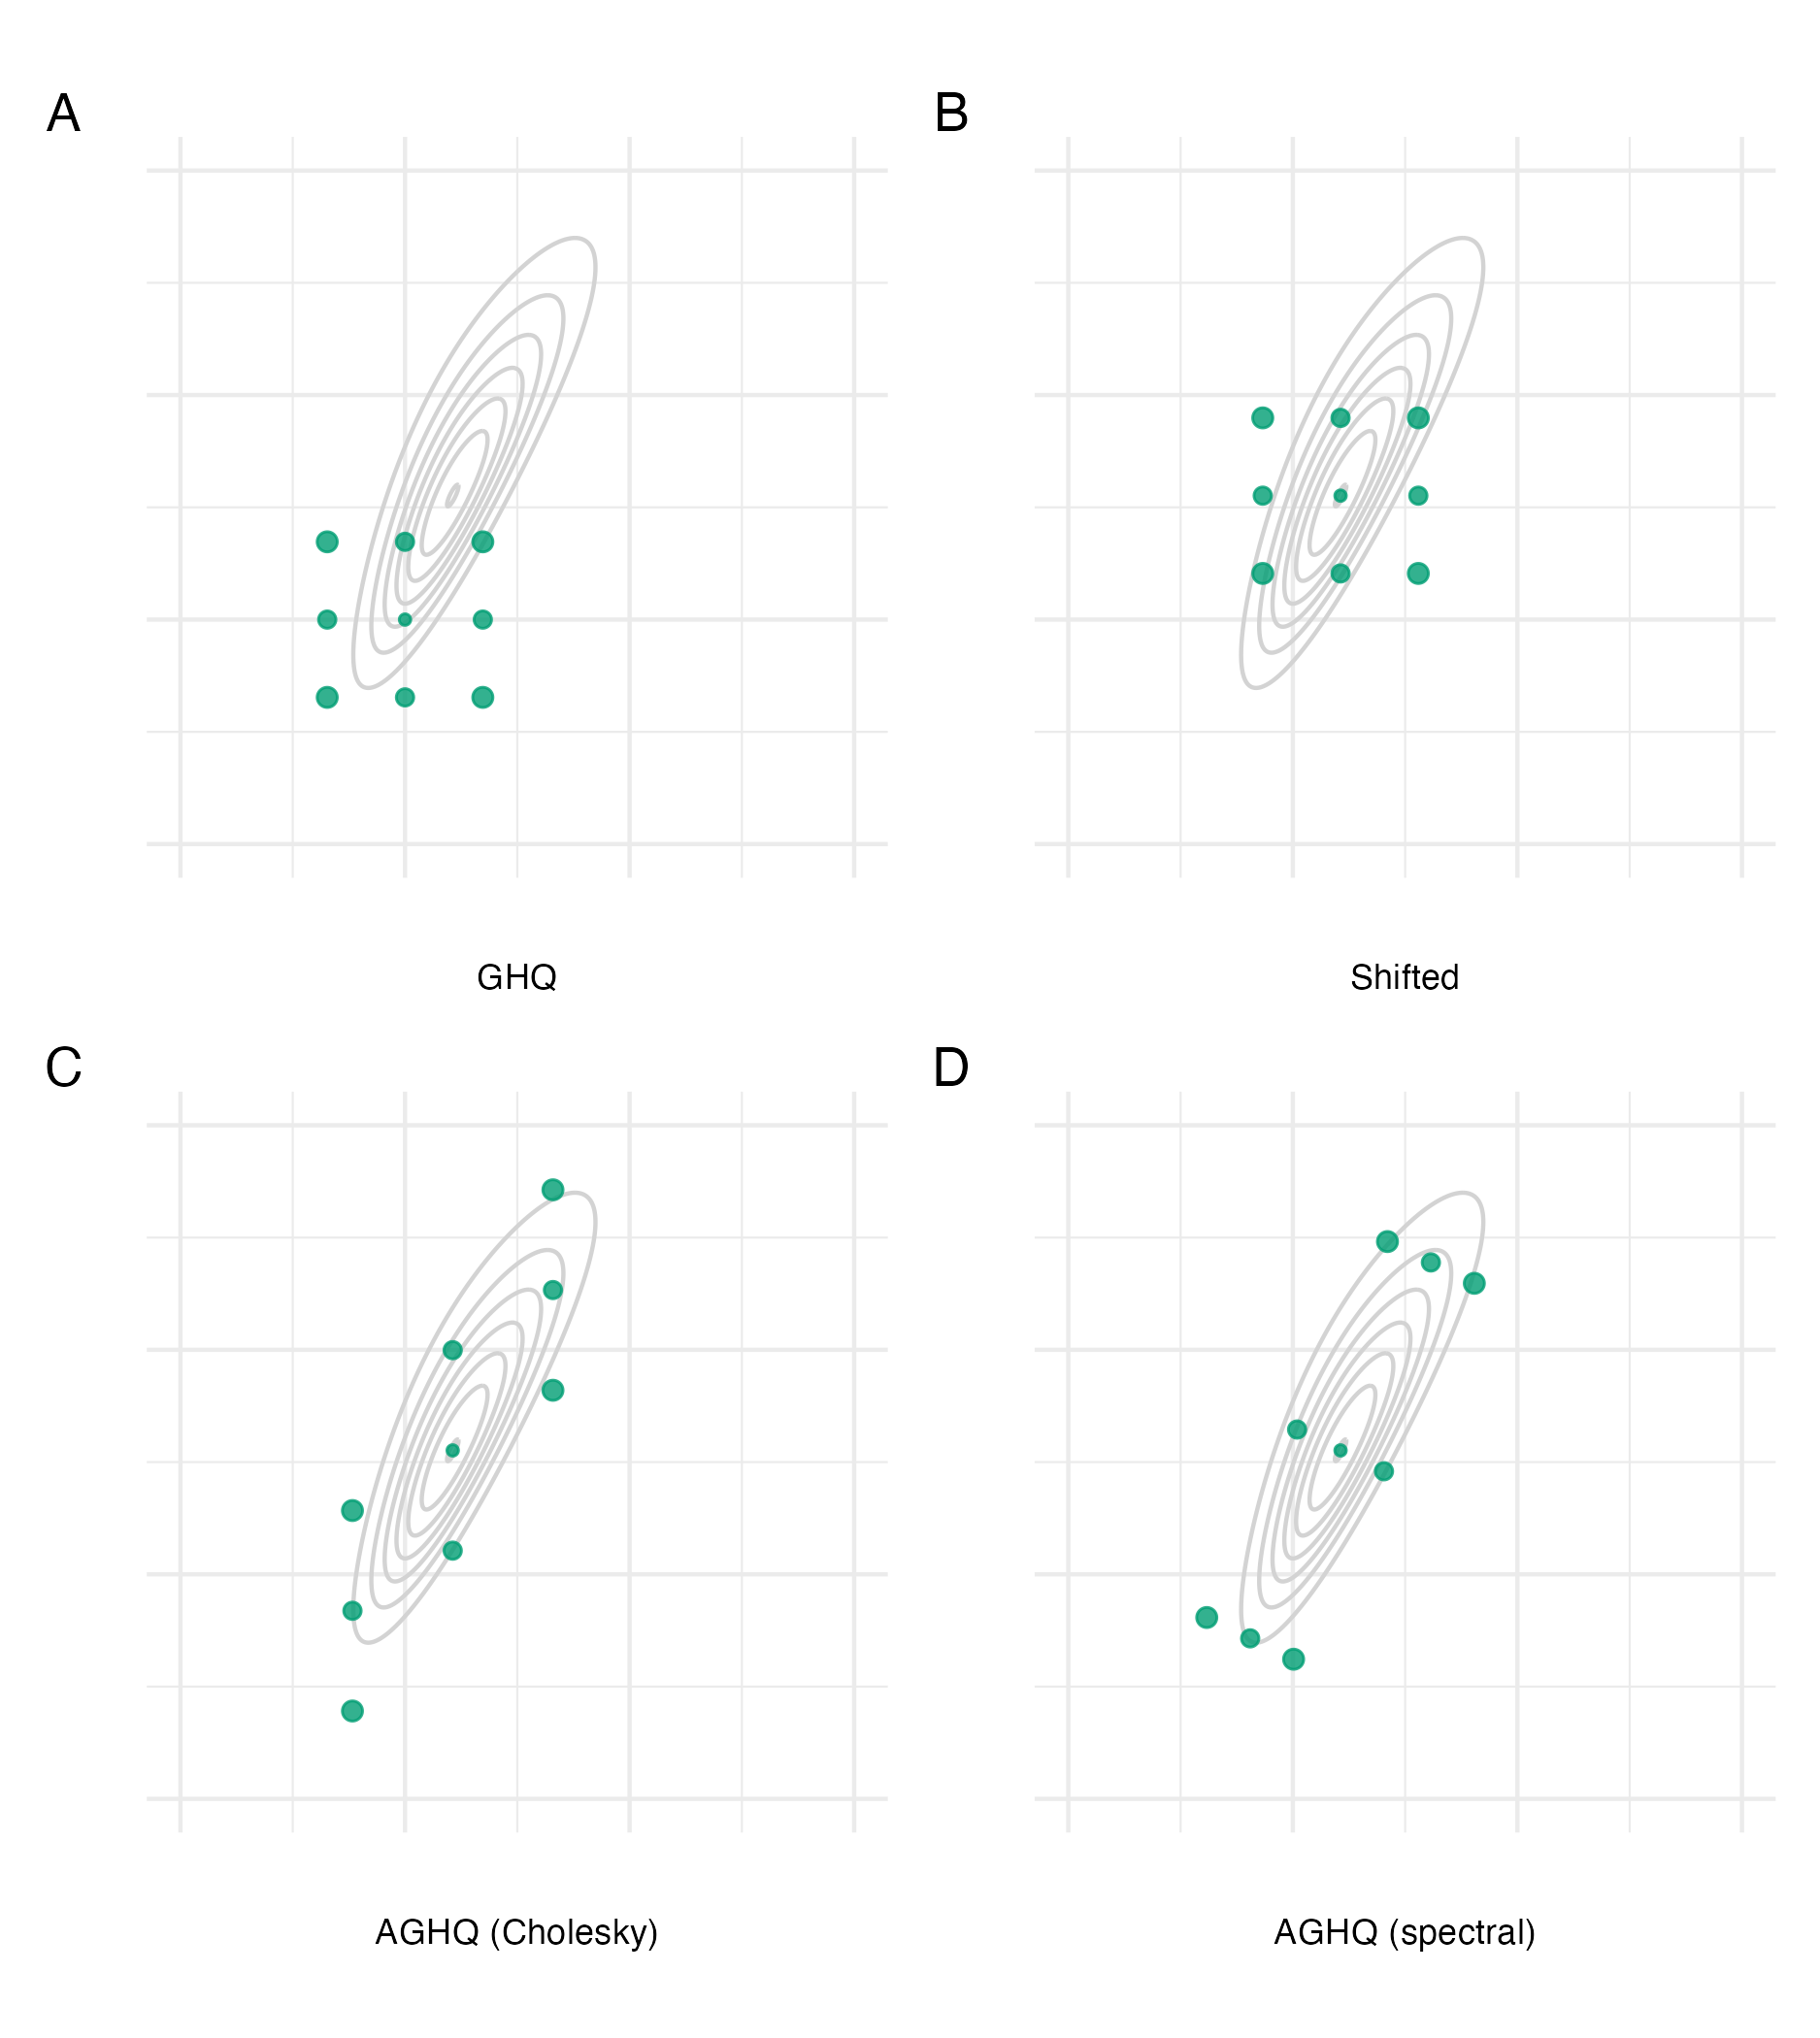
\includegraphics[width=0.95\linewidth]{figures/naomi-aghq/aghq-demo} 

}

\caption{The Gauss-Hermite quadrature nodes \(\mathbf{z} \in \mathcal{Q}(2, 3)\) for a two-dimensional integral with three nodes per dimension (A). Adaption occurs based on the mode (B) and covariance of the integrand via either the Cholesky (C) or spectral (D) decomposition of the inverse curvature at the mode. The integrand is \(f(z_1, z_2) = \text{sn}(0.5 z_1, \alpha = 2) \cdot \text{sn}(0.8 z_1 - 0.5 z_2, \alpha = -2)\), where \(\text{sn}(\cdot)\) is the standard skewnormal probability density function with shape parameter \(\alpha \in \mathbb{R}\).}\label{fig:aghq-demo}
\end{figure}

Two alternatives for the matrix decomposition \autocite{jackel2005note} are the Cholesky and spectral decomposition.
For the Cholesky decomposition \(\hat{\mathbf{P}} = \hat{\mathbf{L}}\), where \(\hat{\mathbf{L}}\) is lower triangular.
For the spectral decomposition \(\hat{\mathbf{P}} = \hat{\mathbf{E}} \hat{\mathbf{\Lambda}}^{1/2}\), where \(\hat{\mathbf{E}} = (\hat{\mathbf{e}}_{1}, \ldots \hat{\mathbf{e}}_{ m})\) contains the eigenvectors of \(\hat{\mathbf{H}}\) and \(\hat{\mathbf{\Lambda}}\) is a diagonal matrix containing its eigenvalues \((\hat \lambda_{1}, \ldots, \hat \lambda_{m})\).
Figure \ref{fig:aghq-demo} demonstrates GHQ and AGHQ for a two-dimensional example, using both decomposition approaches.

\hypertarget{integrated-nested-laplace-approximation}{%
\subsection{Integrated nested Laplace approximation}\label{integrated-nested-laplace-approximation}}

The integrated nested Laplace approximation (INLA) method \autocite{rue2009approximate} combines marginal Laplace approximations with quadrature to enable approximation of posterior marginal distributions.
Consider the marginal Laplace approximation of Section \ref{marginal-la} for a three-stage hierarchical model given by
\begin{equation}
\tilde p_{\texttt{LA}}(\boldsymbol{\mathbf{\theta}}, \mathbf{y}) = \frac{p(\mathbf{y}, \mathbf{x}, \boldsymbol{\mathbf{\theta}})}{\tilde p_\texttt{G}(\mathbf{x} \, | \, \boldsymbol{\mathbf{\theta}}, \mathbf{y})} \Big\rvert_{\mathbf{x} = \hat{\mathbf{x}}(\boldsymbol{\mathbf{\theta}})}.
\end{equation}
The posterior normalising constant may be approximated by integrating the marginal Laplace approximation over the hyperparameters using a quadrature rule.
Following \textcite{stringer2022fast} I consider use of AGHQ.
Let \(\mathbf{z} \in \mathcal{Q}(m, k)\) be the \(m\)-dimensional GHQ nodes with \(k\) nodes per dimension, and \(\omega: \mathbb{R}^m \to \mathbb{R}\) the corresponding weighting function.
Let \(\boldsymbol{\mathbf{\theta}}(\mathbf{z}) = \hat{\mathbf{P}}_\texttt{LA} \mathbf{z} + \hat{\boldsymbol{\mathbf{\theta}}}_\texttt{LA}\) where\ldots{}
\begin{equation}
\tilde p_{\texttt{AQ}}(\mathbf{y}) = \sum_{\mathbf{z} \in \mathcal{Q}(m, k)} \tilde p_\texttt{LA}(\boldsymbol{\mathbf{\theta}}(\mathbf{z}), \mathbf{y}) \omega(\mathbf{z}).
\end{equation}

\hypertarget{gaussian-marginals}{%
\subsubsection{Gaussian marginals}\label{gaussian-marginals}}

\hypertarget{laplace-marginals}{%
\subsubsection{Laplace marginals}\label{laplace-marginals}}

\hypertarget{simplfied-laplace-marginals}{%
\subsubsection{Simplfied Laplace marginals}\label{simplfied-laplace-marginals}}

\textcite{rue2009approximate} use GMRFs.

\hypertarget{simplifed-inla}{%
\subsubsection{Simplifed INLA}\label{simplifed-inla}}

\textcite{wood2020simplified} don't use GMRFs and still do fine.

\hypertarget{software}{%
\section{Software}\label{software}}

\hypertarget{tmb}{%
\subsection{\texorpdfstring{\texttt{TMB}}{TMB}}\label{tmb}}

Template Model Builder {[}TMB, or when referring to the software \texttt{TMB}; \textcite{kristensen2016tmb}{]} is an R package which implements the Laplace approximation.
In \texttt{TMB} derivatives are obtained using automatic differentiation {[}AD; \textcite{baydin2017automatic}{]}.
How does AD work.
Give an example of TMB use.

\hypertarget{r-inla}{%
\subsection{\texorpdfstring{\texttt{R-INLA}}{R-INLA}}\label{r-inla}}

The \texttt{R-INLA} software implements the INLA method.
\texttt{R-INLA} uses a formula interface (e.g.~\texttt{y\ \textasciitilde{}\ 1\ +\ x}) to facilitate use of INLA for common models.
This is a beneficial design choice for new users.
For more advanced users, the formula interface can impose constraints on model choice.
Give an example of \texttt{R-INLA} use.
Finite differences rather than AD.
\texttt{GMRFLib} library.

\hypertarget{a-universal-inla-implementation-based-on-ad}{%
\section{A universal INLA implementation based on AD}\label{a-universal-inla-implementation-based-on-ad}}

In this section, I implement the INLA method, using the \texttt{TMB} package.
This implementation is universal in that it is compatible with any model with a \texttt{TMB} C++ template.
This opens the door for application of INLA to models which are not compatible with \texttt{R-INLA}.
Indeed, \textcite{martino2019integrated} note that ``implementing INLA from scratch is a complex task'' and as a result ``applications of INLA are limited to the (large class of) models implemented {[}in \texttt{R-INLA}{]}''.
The potential benefits of a more flexible INLA implementation based on AD were noted by \textcite{skaug2009approximate} (a coauthors of TMB) in discussion of \textcite{rue2009approximate}, noting that such a system would be ``fast, flexible, and easy-to-use''.
As this suggestion was made close to 15 years ago, it a surprise that its potential remains unrealised.

\hypertarget{epilepsy-example}{%
\subsection{Epilepsy example}\label{epilepsy-example}}

To demonstrate the implementation, consider the epilepsy generalised linear mixed model example of \textcite{spiegelhalter1996bugs}.
This model is based on that of \textcite{breslow1993approximate}, a modification of \textcite{thall1990some}, and the data are from an epilespy drug double-blind clinical trial \autocite{leppik1985double}.
\textcite{rue2009approximate} (Section 5.2) demonstrate the INLA method using this example, and find a significant difference in approximation error depending on use of either the Gaussian or Laplace approximation for some parameters.

In the trial, patients \(i = 1, \ldots, 59\) were each assigned either the new drug \(\texttt{Trt}_i = 1\) or placebo \(\texttt{Trt}_i = 0\).
Each patient made four visits the clinic \(j = 1, \ldots, 4\), and the observations \(y_{ij}\) are the number of seizures of the \(i\)th person in the two weeks preceding their \(j\)th visit.
The covariates used in the model were age \(\texttt{Age}_i\), baseline seizure counts \(\texttt{Base}_i\) and an indicator for the final clinic visit \(\texttt{V}_4\), which were all centered.
The observations were modelled using a Poisson distribution \(y_{ij} \sim \text{Poisson}(e^{\eta_{ij}})\) with linear predictor
\begin{align*}
\eta_{ij}
&= \beta_0 + \beta_\texttt{Base} \log(\texttt{Baseline}_j / 4) + \beta_\texttt{Trt} \texttt{Trt}_i +
   \beta_{\texttt{Trt} \times \texttt{Base}} \texttt{Trt}_i \times \log(\texttt{Baseline}_j / 4) \\ 
&+ \beta_\texttt{Age} \log(\texttt{Age}_i) + \beta_{\texttt{V}_4} {\texttt{V}_4}_j +
   \epsilon_i + \nu_{ij}, \quad i \in [59], \quad j \in [4],
\end{align*}
where the prior distribution on each of the regression parameters, including the intercept, was \(\mathcal{N}(0, 100^2)\).
The random effects are IID \(\epsilon_i \sim \mathcal{N}(0, 1/\tau_\epsilon)\) and \(\nu_{ij} \sim \mathcal{N}(0, 1/\tau_\nu)\) with precision prior distributions \(\tau_\epsilon, \tau_\nu \sim \Gamma(0.001, 0.001)\).

\hypertarget{naomi}{%
\section{The Naomi model}\label{naomi}}

The Naomi small-area estimation model \autocite{eaton2021naomi} synthesises data from multiple sources to estimate HIV indicators at a district-level, by age and sex.

\hypertarget{model-structure}{%
\subsection{Model structure}\label{model-structure}}

I consider a simplified version of Naomi defined only at the time of the most recent household survey with HIV testing.
This version omits nowcasting and temporal projection.
These time points involve limited inferences.

\hypertarget{household-survey-component}{%
\subsubsection{\texorpdfstring{Household survey component \label{sec:household}}{Household survey component }}\label{household-survey-component}}

Consider a country in sub-Saharan Africa where a household survey with complex survey design has taken place.
Let \(x \in \mathcal{X}\) index district, \(a \in \mathcal{A}\) index five-year age group, and \(s \in \mathcal{S}\) index sex.
For ease of notation, let \(i\) index the finest district-age-sex division included in the model.
Let \(I \subseteq \mathcal{X} \times \mathcal{A} \times \mathcal{S}\) be a set of indices \(i\) for which an aggregate observation is reported, and \(\mathcal{I}\) be the set of all \(I\) such that \(I \in \mathcal{I}\).

Let \(N_i \in \mathbb{N}\) be the known, fixed population size.
HIV prevalence \(\rho_i \in [0, 1]\), antiretroviral therapy (ART) coverage \(\alpha_i \in [0, 1]\), and annual HIV incidence rate \(\lambda_i > 0\) are modelled using linked regression equations.

Independent logistic regression models are specified for HIV prevalence and ART coverage in the general population such that \(\text{logit}(\rho_i) = \eta^\rho_i\) and \(\text{logit}(\alpha_i) = \eta^\alpha_i\).
HIV incidence rate is modelled on the log scale as \(\log(\lambda_i) = \eta^\lambda_i\), and depends on adult HIV prevalence and adult ART coverage.
Let \(\kappa_i\) be the proportion recently infected among HIV positive persons.
This proportion is linked to HIV incidence via
\begin{equation}
\kappa_i = 1- \exp \left( - \lambda_i \cdot \frac{1 - \rho_i}{\rho_i} \cdot (\Omega_T - \beta_T) - \beta_T \right), \label{eq:kappa}
\end{equation}
where the mean duration of recent infection \(\Omega_T\) and the proportion of long-term HIV infections misclassified as recent \(\beta_T\) are strongly informed by priors for the particular survey.

These processes are each informed by household survey data.
Weighted aggregate survey observations are calculated as
\begin{equation*}
\hat \theta_I = \frac{\sum_j w_j \cdot\theta_j}{\sum_j w_j},
\end{equation*}
with individual responses \(\theta_j \in \{0, 1\}\) and design weights \(w_j\) for each of \(\theta \in \{\rho, \alpha, \kappa\}\).
The design weights are provided by the survey and aim to reduce bias by decreasing possible correlation between response and recording mechanism \autocite{meng2018statistical}.
The index \(j\) runs across all individuals in strata \(i \in I\) within the relevant denominator i.e.~for ART coverage, only those individuals who are HIV positive.
The weighted observed number of outcomes is \(y^{\theta}_{I} = m^{\theta}_{I} \cdot \hat \theta_{I}\) where
\begin{equation*}
m^{\theta}_I = \frac{\left(\sum_j w_j\right)^2}{\sum_j w_j^2},
\end{equation*}
is the Kish effective sample size (ESS) \autocite{kish1965survey}.
As the Kish ESS is maximised by constant design weights, in exchange for reducing bias the ESS is reduced and hence variance increased.
The weighted observed number of outcomes are modelled using a binomial working likelihood \autocite{chen2014use} defined to operate on the reals
\begin{equation*}
y^{\theta}_{I} \sim \text{xBin}(m^{\theta}_{I}, \theta_{I}),
\end{equation*}
where \(\theta_{I}\) are the following weighted aggregates
\begin{equation*}
\rho_{I} = \frac{\sum_{i \in I} N_i \rho_i}{\sum_{i \in I} N_i}, \quad
\alpha_{I} = \frac{\sum_{i \in I} N_i \rho_i \alpha_i}{\sum_{i \in I} N_i \rho_i}, \quad
\kappa_{I} = \frac{\sum_{i \in I} N_i \rho_i \kappa_i}{\sum_{i \in I} N_i \rho_i}.
\end{equation*}

\hypertarget{connection-to-elgms}{%
\subsection{Connection to ELGMs}\label{connection-to-elgms}}

\hypertarget{extending-aghq-to-moderate-dimensions}{%
\section{Extending AGHQ to moderate dimensions}\label{extending-aghq-to-moderate-dimensions}}

The Naomi model has \(m = 24\) hyperparameters.
AGHQ with the product rule grid requries evaluation of \(|\mathcal{Q}(m, k)| = k^m\) quadrature points.
This is intractable for \(m = 24\).
This section focuses on the development of AGHQ rules for moderate dimensions, for use within the nested Laplace approximation algorithm.

\hypertarget{aghq-with-variable-levels}{%
\subsection{AGHQ with variable levels}\label{aghq-with-variable-levels}}

Let \(\mathbf{k} = (k_1, \ldots, k_m)\) be a vector of levels for each dimension of \(\boldsymbol{\mathbf{\theta}}\).
We may then define \(\mathcal{Q}(m, \mathbf{k}) = \mathcal{Q}(1, k_1) \times \cdots \times \mathcal{Q}(1, k_m)\) to be a GHQ grid with possible variable levels of size \(|\mathcal{Q}(m, \mathbf{k})| = \prod_{j = 1}^m k_j\).
Let \(\mathcal{Q}(m, s, k)\) correspond to \(\mathcal{Q}(m, \mathbf{k})\) with choice of levels \(k_j = k, j \leq s\) and \(k_j = 1, j > s\) for some \(s \leq m\).
For example, for \(m = 2\) and \(s = 1\) then \(\mathbf{k} = (k, 1)\).
In combination with use of the spectral decomposition, this choice of levels is analogous to a principal components analysis (PCA) approach to AGHQ.
We refer to this approach as PCA-AGHQ, with corresponding estimate of the normalising constant given by
\begin{equation}
\tilde p_\texttt{PCA}(\mathbf{y}) = |\hat{\mathbf{E}}_{\texttt{LA}} \hat{\mathbf{\Lambda}}_{\texttt{LA}}^{1/2}|\sum_{\mathbf{z} \in \mathcal{Q}(m, s, k)} \tilde p_\texttt{LA}(\hat{\mathbf{E}}_{\texttt{LA}, s} \hat{\mathbf{\Lambda}}_{\texttt{LA}, s}^{1/2} \mathbf{z} + \hat{\boldsymbol{\mathbf{\theta}}}_\texttt{LA}, \mathbf{y}) \omega(\mathbf{z}),
\end{equation}
where \(\hat{\mathbf{E}}_{\texttt{LA}, s}\) is an \(m \times s\) matrix containing the first \(s\) eigenvectors, \(\hat{\mathbf{\Lambda}}_{\texttt{LA}, s}\) is the \(s \times s\) diagonal matrix containing the first \(s\) eigenvalues, and \(\omega(\mathbf{z}) = \prod_{j = 1}^s \omega_s(z_j) \times \prod_{j = s + 1}^d \omega_1(z_j)\).
Panel C of Figure \ref{fig:aghq} illustrates PCA-AGHQ for a case when \(m = 2\) and \(s = 1\).
As AGHQ with \(k = 1\) corresponds to the Laplace approximation, PCA-AGHQ can be interpreted as performing AGHQ on the first \(s\) principal components of the inverse curvature, and a Laplace approximation on the remaining \(m - s\) principal components.
Inference for the latent field follows analogously to Equation \ref{eq:nest}.

\hypertarget{principal-components-analysis}{%
\subsection{Principal components analysis}\label{principal-components-analysis}}



\begin{figure}

{\centering 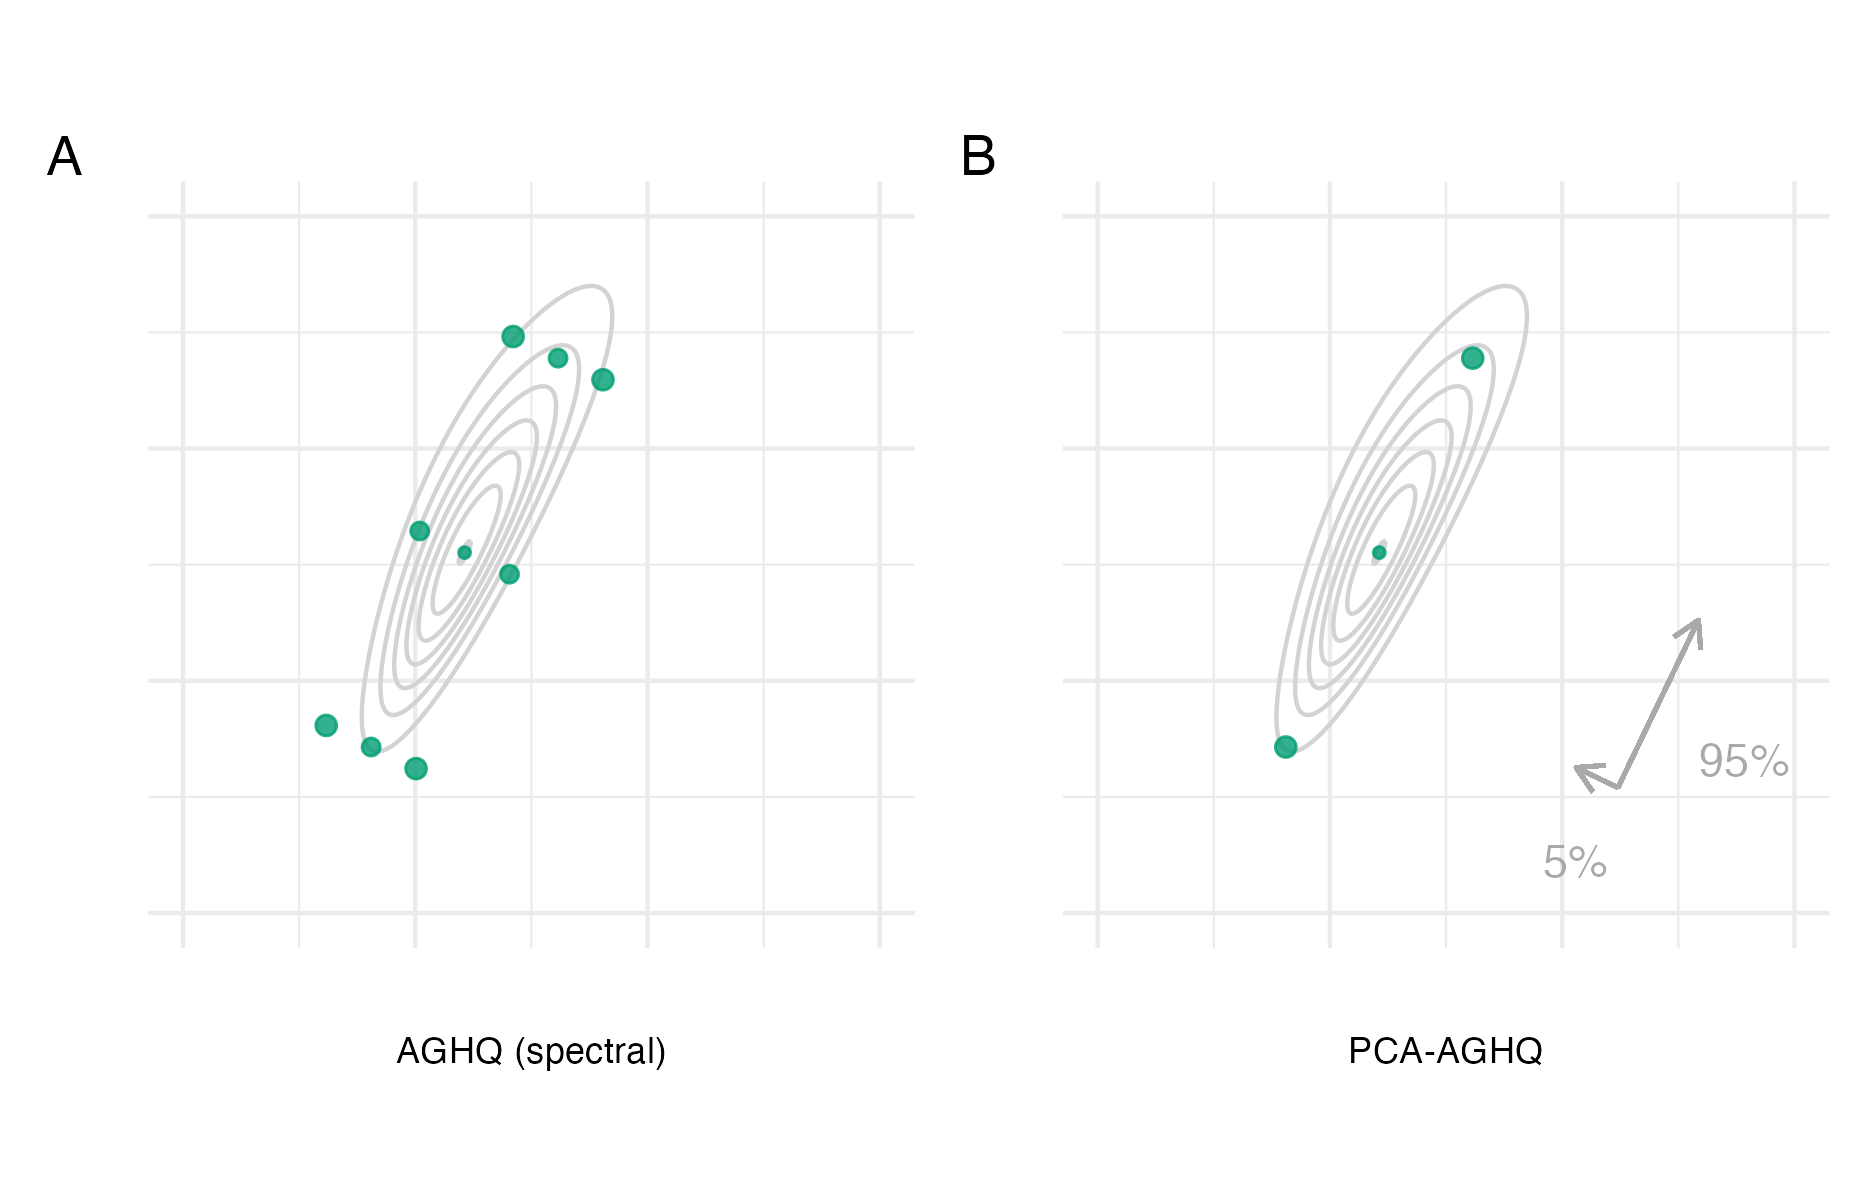
\includegraphics[width=0.95\linewidth]{figures/naomi-aghq/pca-demo} 

}

\caption{See Figure \ref{fig:aghq-demo}.}\label{fig:pca-demo}
\end{figure}

\hypertarget{malawi-case-study}{%
\section{Malawi case-study}\label{malawi-case-study}}



\begin{figure}

{\centering 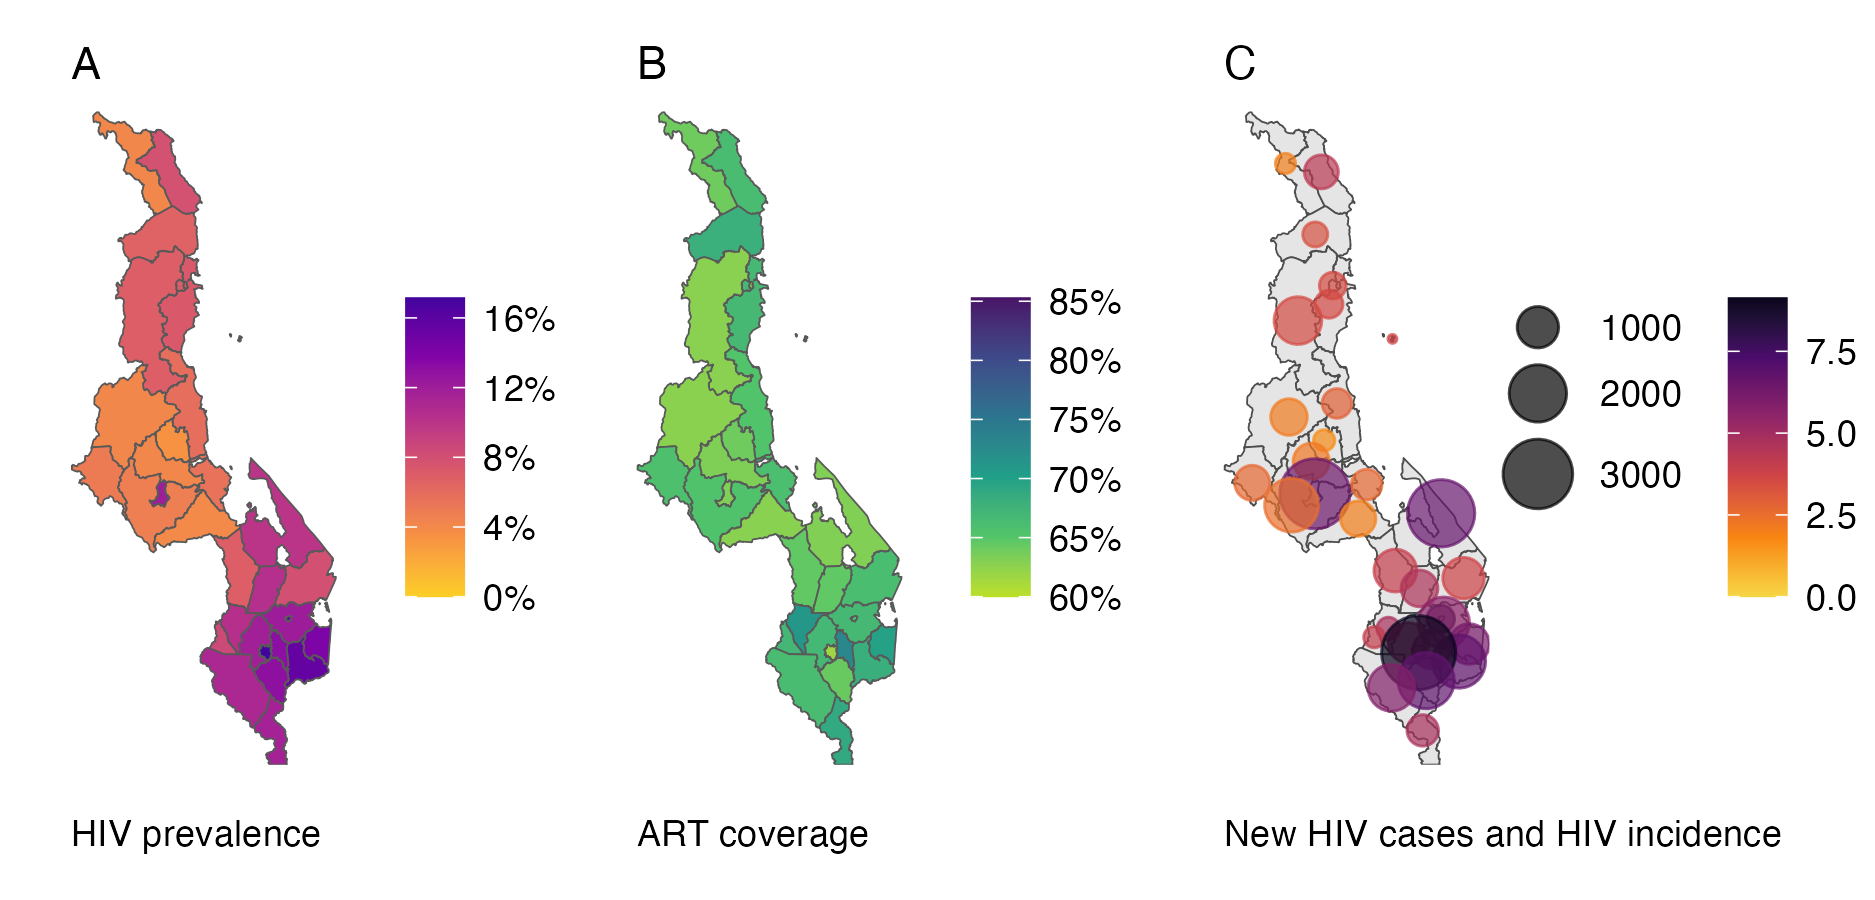
\includegraphics[width=0.95\linewidth]{resources/naomi-aghq/20230811-095752-5b8181d8/depends/figB} 

}

\caption{Figure caption.}\label{fig:naomi-output}
\end{figure}

The Naomi model, as described in Section \ref{naomi}, was fit to data from Malawi using three inferential approaches.

\hypertarget{nuts-convergence}{%
\subsection{NUTS convergence}\label{nuts-convergence}}

\hypertarget{use-of-pca-aghq}{%
\subsection{Use of PCA-AGHQ}\label{use-of-pca-aghq}}

\hypertarget{model-assessment}{%
\subsection{Model assessment}\label{model-assessment}}

\hypertarget{inference-comparison}{%
\subsection{Inference comparison}\label{inference-comparison}}

\hypertarget{exceedance-probabilities}{%
\subsection{Exceedance probabilities}\label{exceedance-probabilities}}

\hypertarget{discussion-2}{%
\section{Discussion}\label{discussion-2}}

We developed an approximate Bayesian inference algorithm, combining AGHQ with PCA, motivated by a challenging problem in small-area estimation of HIV indicators.
For the simplified Naomi model in Malawi (Section \ref{sec:results}) we demonstrated the method to be more accurate at inferring posterior distributions of model parameters, across a broad range of metrics, than TMB, and substantially faster than NUTS.
However, improvements in accuracy for model parameters did not translate into model outputs.
Indeed, we found posterior exceedance probabilities (Section \ref{sec:exceedance}) from both TMB and PCA-AGHQ to have systematically inaccuracies, with the potential to meaningfully mislead policy.
If possible, though not a desirable situation, it could be advisable to provide gold-standard NUTS results after the workshop has concluded.
However, running NUTS for Naomi took days, in countries with 100s of districts it may simply not be feasible.

PCA-AGHQ could be added to the Naomi web interface as an alternative to TMB.
Analysts may then quickly iterate over model options using a fast inference approach, before switching to a more accurate approach once they are happy with the results.
By selecting \(s\) and \(k\), PCA-AGHQ can be adjusted to suit the computational budget available.
We selected \(s\) based on the Scree plot, and for the most part fixed \(k = 3\).
Whether it is preferable, for a given computational budget, to increase \(s\) or increase \(k\) is an open question.
Further strategies, such as gradually lowering \(k\) over the principal components, could also be considered.

We hope that our work further encourages use of deterministic inference algorithms for ELGMs in applied settings, as well as methodological exploration of their accuracy and limitations.
Among the ELGM-type structures of particular interest in spatial epidemiology are aggregated Gaussian process models \autocite{nandi2020disaggregation} and evidence synthesis models \autocite{amoah2020geostatistical}.

\hypertarget{suggestions-for-future-work}{%
\subsection{Suggestions for future work}\label{suggestions-for-future-work}}

\hypertarget{improved-quadrature-grids-for-moderate-dimensions}{%
\subsubsection{Improved quadrature grids for moderate dimensions}\label{improved-quadrature-grids-for-moderate-dimensions}}

We aimed to develop a quadrature grid which allocates more effort to more important dimensions.
While PCA is a sensible approach, there are avenues where it does not behave as one might hope, or otherwise overlooks potential benefits.
The first challenge we identified was using PCA when the dimensions have different scales.
Specifically, we found logit-scale hyperparamters to be systematically favoured over those on the log-scale.
Second, the amount of variation explained for the Hessian matrix is not of directly interest, rather the effect of the different dimensions on the relevant outputs.
Using measures of importance from sensitivity analysis, such as Shapley values \autocite{shapley1953value} may be preferable.
Third, it is more important to allocate quadrature nodes to those marginals which are non-Gaussian.
This is because the Laplace approximation is exact when the integrand is Gaussian, so a single quadrature node is sufficiently.
The difficulty is, of course, knowing in advance which marginals will be non-Gaussian.
This could be done if there were a cheap way to obtain posterior means, which could then be compared to posterior modes obtained using optimisation.
Another approach would be to measure the fit of marginal samples from a cheap approximation, like TMB.
The main challenge is that the measurements have to for marginals, ruling out approaches like PSIS which operate on joint distributions \autocite{yao2018yes}.

\hypertarget{computational-speed-ups}{%
\subsubsection{Computational speed-ups}\label{computational-speed-ups}}

Integration over a moderate number of hyperparameters posed a challenge, and led us to use a quadrature grids with a large number of nodes.
However, computation at each node is independent, such that the run-time of the algorithm could potentially be significantly improved by parallel computing.
Further computational speed-ups might be obtained using graphics processing units (GPUs) speciallised for the relevant matrix operations.

\hypertarget{comparison-to-other-mcmc-algorithms}{%
\subsubsection{Comparison to other MCMC algorithms}\label{comparison-to-other-mcmc-algorithms}}

Blocked Gibbs sampling \autocite{geman1984stochastic} or slice sampling \autocite{neal2003slice}, may be better suited than NUTS to sampling from Naomi.
These algorithms are available, and customisable, including e.g.~choice of block structure within the \texttt{NIMBLE} probabilistic programming language \autocite{de2017programming}.

\hypertarget{implementation-into-probabilistic-programming-languages}{%
\subsubsection{Implementation into probabilistic programming languages}\label{implementation-into-probabilistic-programming-languages}}

Though gaining in popularity, the user-base of \texttt{TMB} remains relatively small.
Furthermore, for users unfamiliar with C++, it can be challenging to use.
As such, it could be beneficial to implement AGHQ within other probabilistic programming languages.
Implementation in \texttt{NIMBLE} could be relatively straightforward, as it (for version \textgreater1.0.0) includes functionality for automatic differentiation and Laplace approximation, built using \texttt{CppAD} like \texttt{TMB}.
Similarly, implementation in Stan could be possible by use of the \texttt{bridgestan} package \autocite{bridgestan} together with the adjoint-differentiated Laplace approximation of \textcite{margossian2020hamiltonian}.

\hypertarget{statistical-theory}{%
\subsubsection{Statistical theory}\label{statistical-theory}}

\textcite{stringer2022fast} (Theorem 1) bound the total variation error of AGHQ, establishing convergence in probability of coverage probabilities under the approximate posterior to those under the true posterior.
Similar theory might be established for PCA-AGHQ, or more generally AGHQ with varying numbers of nodes per dimension.
The challenge of connecting this theory to use of the quadrature rule within nested compuations remains an open question.

\hypertarget{conclusions}{%
\chapter{Future work and conclusions}\label{conclusions}}

\adjustmtc
\markboth{Conclusions}{}

\hypertarget{strengths}{%
\section{Strengths}\label{strengths}}

\hypertarget{chapter-refbeyond-borders}{%
\subsection{Chapter \ref{beyond-borders}}\label{chapter-refbeyond-borders}}

\begin{itemize}
\tightlist
\item
  I designed experiments to thoroughly compare models for spatial structure using tools for model assessment such as proper scoring rules and posterior predictive checks.
\end{itemize}

\hypertarget{chapter-refmulti-agyw}{%
\subsection{Chapter \ref{multi-agyw}}\label{chapter-refmulti-agyw}}

\begin{itemize}
\tightlist
\item
  I estimated HIV risk group proportions for AGYW, enabling countries to prioritise their delivery of HIV prevention services.
\item
  I analysed the number of new infections that might be reached under a variety of risk stratification strategies.
\item
  I used \texttt{R-INLA} to specify multinomial spatio-temporal models via the Poisson-multinomial transformation. This includes complex two- and three-way Kronecker product interactions defined using the \texttt{group} and \texttt{replicate} options.
\end{itemize}

\hypertarget{chapter-refnaomi-aghq}{%
\subsection{Chapter \ref{naomi-aghq}}\label{chapter-refnaomi-aghq}}

\begin{itemize}
\tightlist
\item
  I developed a novel Bayesian inference method, motivated by a challenging and practically important problem in HIV inference.
\item
  The method enables integrated nested Laplace approximations to be fit to and studied on a wider class of models than was previously possible.
\item
  My implementation of the method was straightforward, building on the \texttt{TMB} and \texttt{aghq} packages, and described completely and accessibly in \textcite{howes2023fast}.
\end{itemize}

\hypertarget{future-work}{%
\section{Future work}\label{future-work}}

Avenues for future work include:

\begin{enumerate}
\def\labelenumi{\arabic{enumi}.}
\tightlist
\item
  Extending the risk group model described in Chapter \ref{multi-agyw} to include all adults 15-49. This may involve modelling of age-stratified sexual partnerships \autocite{wolock2021evaluating}.
  Such a model would likely fall out of the scope of \texttt{R-INLA}, but would be possible to write with \texttt{TMB} and therefore amenable to the methods discussed in Chapter \ref{naomi-aghq}.
\item
  Speeding up the implementation of Laplace marginals using the matrix algebra approximations described in \textcite{wood2020simplified}.
\item
  Evaluating the accuracy of deterministic Bayesian inference methods for a broader variety of extended latent Gaussian models.
\end{enumerate}

\hypertarget{conclusions-1}{%
\section{Conclusions}\label{conclusions-1}}

\begin{itemize}
\tightlist
\item
  Modelling complex data, more often than not, pushes the boundaries of the statistical toolkit available.
\item
  A challenge I encountered was the difficulty of implementing identical models across multiple frameworks with the aim of studying the inference method. Or, of a similarly fraught nature, comparing different models implemented in different frameworks with the aim of studying model differences. The frequently asked questions section of the \texttt{R-INLA} website \autocite{rinla2023faq} notes that ``the devil is in the details''. I have resolved this challenge by using a given \texttt{TMB} model template to fit models using multiple inference methodologies. The benefits of such a ecosystem of packages are noted by \textcite{stringer2021fields}. I particularly highlight the benefit of enabling analysts to easily vary their choice of inference method based on the stage of model development that they are in.
\item
  To the best of my abilities, I have written this thesis, and the work described within it, in keeping with the principles of open science. I hope that doing so allows my work to be scrutinised, and optimistically built upon. This would not have been possible without a range of tools from the R ecosystem such as \texttt{rmarkdown} and \texttt{rticles}, as well as those developed within the MRC Centre for Global Infectious Disease Analysis such as \texttt{orderly} and \texttt{didehpc}.
\end{itemize}

\startappendices

\hypertarget{models-for-spatial-structure}{%
\chapter{Models for spatial structure}\label{models-for-spatial-structure}}

\hypertarget{a-model-for-risk-group-proportions}{%
\chapter{A model for risk group proportions}\label{a-model-for-risk-group-proportions}}

\hypertarget{the-global-aids-strategy}{%
\section{The Global AIDS Strategy}\label{the-global-aids-strategy}}

\begin{table}[h]
\centering
\begin{tabularx}{\textwidth}{lX}
\toprule
Prioritisation strata & Criterion  \\
\midrule
Low & 0.3-1.0\% incidence and low-risk behaviour, or $<$0.3\% incidence and high-risk behaviour \\
Moderate & 1.0-3.0\% incidence and low-risk behaviour, or 0.3-1.0\% incidence and high-risk behaviour \\
High & 1.0-3.0\% incidence and high-risk behaviour \\
Very high & $>$3.0\% incidence \\
\bottomrule
\end{tabularx}
\caption{Prioritisation strata according to HIV incidence in the general population and behavioural risk.}
\label{tab:unaids-strategy-prioritisation}
\end{table}

\begin{table}[h]
\centering
\begin{tabularx}{\textwidth}{p{8cm}XXXX}
\toprule
Intervention & Low & Moderate & High & Very High \\
\midrule
Condoms and lube for those with non-regular partners(s) with unknown STI status and not on PrEP & 50\% & 70\% & 95\% & 95\% \\
STI screening and treatment & 10\% & 10\% & 80\% & 80\% \\
Access to PEP & - & - & 50\% & 90\% \\
PrEP use & - & 5\% & 50\% & 50\% \\
Economic empowerment & - & - & 20\% & 20\% \\
\bottomrule
\end{tabularx}
\caption{Commitments to be met for each intervention in terms of proportion of the prioritisation strata reached. The symbol "-" represents no commitment.}
\label{tab:unaids-strategy-targets}
\end{table}

\hypertarget{household-survey-data}{%
\section{Household survey data}\label{household-survey-data}}

\begin{longtable}{rlrcrrrr}
\toprule
\multicolumn{1}{l}{} &  &  &  & \multicolumn{4}{c}{Sample size} \\ 
\cmidrule(lr){5-8}
\multicolumn{1}{l}{} & Type & Year & Transactional sex question & 15-19 & 20-24 & 25-29 & Total \\ 
\midrule
\multicolumn{1}{l}{Botswana} \\ 
\midrule
 & BAIS & 2013 & \cmark & 557 & 588 & 649 & 1794 \\ 
Total &  &  &  & $557$ & $588$ & $649$ & $1794$ \\ 
\midrule
\multicolumn{1}{l}{Cameroon} \\ 
\midrule
 & DHS & 2004 & \xmark & 2675 & 2207 & 1732 & 6614 \\ 
 & DHS & 2011 & \xmark & 3588 & 3115 & 2655 & 9358 \\ 
 & PHIA & 2017 & \xmark & 2620 & 2339 & 2259 & 7218 \\ 
 & DHS & 2018 & \cmark & 3349 & 2463 & 2345 & 8157 \\ 
Total &  &  &  & $12232$ & $10124$ & $8991$ & $31347$ \\ 
\midrule
\multicolumn{1}{l}{Kenya} \\ 
\midrule
 & DHS & 2003 & \xmark & 1819 & 1709 & 1391 & 4919 \\ 
 & DHS & 2008 & \xmark & 1767 & 1743 & 1419 & 4929 \\ 
 & DHS & 2014 & \xmark & 2861 & 2534 & 2858 & 8253 \\ 
Total &  &  &  & $6447$ & $5986$ & $5668$ & $18101$ \\ 
\midrule
\multicolumn{1}{l}{Lesotho} \\ 
\midrule
 & DHS & 2004 & \xmark & 1761 & 1455 & 1026 & 4242 \\ 
 & DHS & 2009 & \xmark & 1833 & 1543 & 1194 & 4570 \\ 
 & DHS & 2014 & \xmark & 1537 & 1292 & 1067 & 3896 \\ 
 & PHIA & 2017 & \cmark & 1156 & 1202 & 1054 & 3412 \\ 
Total &  &  &  & $6287$ & $5492$ & $4341$ & $16120$ \\ 
\midrule
\multicolumn{1}{l}{Mozambique} \\ 
\midrule
 & AIS & 2009 & \xmark & 1031 & 1106 & 987 & 3124 \\ 
 & DHS & 2011 & \xmark & 2932 & 2299 & 2206 & 7437 \\ 
 & AIS & 2015 & \xmark & 1552 & 1389 & 1080 & 4021 \\ 
Total &  &  &  & $5515$ & $4794$ & $4273$ & $14582$ \\ 
\midrule
\multicolumn{1}{l}{Malawi} \\ 
\midrule
 & DHS & 2000 & \xmark & 2914 & 2998 & 2358 & 8270 \\ 
 & DHS & 2004 & \xmark & 2407 & 2823 & 2135 & 7365 \\ 
 & DHS & 2010 & \xmark & 5031 & 4387 & 4309 & 13727 \\ 
 & DHS & 2015 & \cmark & 5273 & 5094 & 3976 & 14343 \\ 
 & PHIA & 2016 & \cmark & 1646 & 1934 & 1511 & 5091 \\ 
Total &  &  &  & $17271$ & $17236$ & $14289$ & $48796$ \\ 
\midrule
\multicolumn{1}{l}{Namibia} \\ 
\midrule
 & DHS & 2000 & \xmark & 1427 & 1313 & 1098 & 3838 \\ 
 & DHS & 2006 & \xmark & 2203 & 1869 & 1544 & 5616 \\ 
 & DHS & 2013 & \xmark & 1852 & 1709 & 1481 & 5042 \\ 
 & PHIA & 2017 & \cmark & 1491 & 1525 & 1370 & 4386 \\ 
Total &  &  &  & $6973$ & $6416$ & $5493$ & $18882$ \\ 
\midrule
\multicolumn{1}{l}{Eswatini} \\ 
\midrule
 & DHS & 2006 & \xmark & 1265 & 1027 & 731 & 3023 \\ 
 & PHIA & 2017 & \xmark & 1031 & 895 & 811 & 2737 \\ 
Total &  &  &  & $2296$ & $1922$ & $1542$ & $5760$ \\ 
\midrule
\multicolumn{1}{l}{Tanzania} \\ 
\midrule
 & AIS & 2003 & \xmark & 1466 & 1377 & 1270 & 4113 \\ 
 & AIS & 2007 & \xmark & 2137 & 1676 & 1509 & 5322 \\ 
 & DHS & 2010 & \xmark & 2221 & 1860 & 1613 & 5694 \\ 
 & AIS & 2012 & \xmark & 2474 & 1923 & 1815 & 6212 \\ 
 & PHIA & 2016 & \cmark & 2999 & 2845 & 2521 & 8365 \\ 
Total &  &  &  & $11297$ & $9681$ & $8728$ & $29706$ \\ 
\midrule
\multicolumn{1}{l}{Uganda} \\ 
\midrule
 & DHS & 2000 & \xmark & 1687 & 1541 & 1326 & 4554 \\ 
 & DHS & 2006 & \xmark & 1948 & 1660 & 1404 & 5012 \\ 
 & AIS & 2011 & \xmark & 2451 & 2164 & 1921 & 6536 \\ 
 & DHS & 2011 & \xmark & 2025 & 1664 & 1614 & 5303 \\ 
 & DHS & 2016 & \cmark & 4276 & 3782 & 3014 & 11072 \\ 
 & PHIA & 2016 & \xmark & 3289 & 3059 & 2574 & 8922 \\ 
\midrule 
Total &  &  &  & $15676$ & $13870$ & $11853$ & $41399$ \\ 
\midrule
\multicolumn{1}{l}{South Africa} \\ 
\midrule
 & DHS & 2016 & \cmark & 1505 & 1408 & 1397 & 4310 \\ 
Total &  &  &  & $1505$ & $1408$ & $1397$ & $4310$ \\ 
\midrule
\multicolumn{1}{l}{Zambia} \\ 
\midrule
 & DHS & 2007 & \xmark & 1598 & 1405 & 1373 & 4376 \\ 
 & DHS & 2013 & \xmark & 3685 & 3036 & 2789 & 9510 \\ 
 & PHIA & 2016 & \cmark & 2120 & 2045 & 1619 & 5784 \\ 
 & DHS & 2018 & \cmark & 3112 & 2687 & 2166 & 7965 \\ 
Total &  &  &  & $10515$ & $9173$ & $7947$ & $27635$ \\ 
\midrule
\multicolumn{1}{l}{Zimbabwe} \\ 
\midrule
 & DHS & 1999 & \xmark & 1467 & 1230 & 1011 & 3708 \\ 
 & DHS & 2005 & \xmark & 2128 & 1943 & 1438 & 5509 \\ 
 & DHS & 2010 & \xmark & 1963 & 1796 & 1679 & 5438 \\ 
 & DHS & 2015 & \cmark & 2154 & 1777 & 1646 & 5577 \\ 
 & PHIA & 2016 & \cmark & 2114 & 1817 & 1573 & 5504 \\ 
Total &  &  &  & $9826$ & $8563$ & $7347$ & $25736$ \\ 
\midrule 
\midrule 
Total &  &  &  & $106397$ & $95253$ & $82518$ & $284168$ \\ 
\bottomrule
\caption{All of the surveys that used in the analysis and their sample sizes, disaggregated by respondent age.}
\label{tab:surveys-used}
\end{longtable}

\begin{table}[h]
\centering
\begin{tabularx}{\textwidth}{lX}
\toprule
Survey & Exclusion reason \\ 
 \midrule
MOZ2003DHS & No GPS coordinates available to place survey clusters within districts. \\
TZA2015DHS & Insufficient sexual behaviour questions. \\
UGA2004AIS & Unable to download region boundaries. \\
ZMB2002DHS & No GPS coordinates available to place survey clusters within districts. \\
\bottomrule
\end{tabularx}
\label{tab:surveys-excluded}
\caption{All of that surveys that were excluded from the analysis.}
\end{table}

\hypertarget{spatial-analysis-levels}{%
\section{Spatial analysis levels}\label{spatial-analysis-levels}}

\begin{table}[h]
\centering
\begin{tabularx}{\textwidth}{lXX}
\toprule
Country & Number of areas & Analysis level \\ 
\midrule
Botswana & 27 & 3 \\ 
Cameroon & 58 & 2 \\ 
Kenya & 47 & 2 \\ 
Lesotho & 10 & 1 \\ 
Mozambique & 161 & 3 \\ 
Malawi & 33 & 5 \\ 
Namibia & 38 & 2 \\ 
Eswatini & 4 & 1 \\ 
Tanzania & 195 & 4 \\ 
Uganda & 136 & 3 \\ 
South Africa & 52 & 2 \\ 
Zambia & 116 & 2 \\ 
Zimbabwe & 63 & 2 \\ 
\bottomrule
\end{tabularx}
\label{tab:area-levels}
\caption{The numer of areas and analysis levels for each country that were used in the analysis.}
\end{table}

\hypertarget{survey-questions}{%
\section{Survey questions and risk group allocation}\label{survey-questions}}

\begin{table}[h]
\centering
\begin{tabularx}{\textwidth}{lX}
\toprule
Variable(s) & Description \\
\midrule
\texttt{v501} & Current marital status of the respondent. \\
\texttt{v529} & Computed time since last sexual intercourse. \\
\texttt{v531} & Age at first sexual intercourse--imputed. \\
\texttt{v766b} & Number of sexual partners during the last 12 months (including husband). \\
\texttt{v767[a, b, c]} & Relationship with last three sexual partners. Options are: spouse, boyfriend not living with respondent, other friend, casual acquaintance, relative, commercial sex worker, live-in partner, other. \\
\texttt{v791a} & Had sex in return for gifts, cash or anything else in the past 12 months. Asked only to women 15-24 who are not in a union. \\
\bottomrule
\end{tabularx}
\caption{The survey questions included in AIDS Indicator Survey (AIS) and Demographic and Health Surveys (DHS).}
\end{table}

\begin{table}[h]
\centering
\begin{tabularx}{\textwidth}{lX}
\toprule
Variable(s) & Description \\
\midrule
\texttt{part12monum} & Number of sexual partners during the last 12 months (including husband). \\
\texttt{part12modkr} & Reason for leaving \texttt{part12monum} blank. \\
\texttt{partlivew[1, 2, 3]} & Does the person you had sex with live in this household? \\
\texttt{partrelation[1, 2, 3]} & Relationship with last three sexual partners. Options are: husband, live-in partner, partner (not living with), ex-spouse/partner, friend/acquaintance, sex worker, sex worker client, stranger, other, don't know, refused. \\
\texttt{sellsx12mo} & Had sex for money and/or gifts in the last 12 months. \\
\texttt{buysx12mo} & Paid money or given gifts for sex in the last 12 months. \\
\bottomrule
\end{tabularx}
\caption{The survey questions included in Population-Based HIV Impact Assessment (PHIA) surveys.}
\end{table}

\hypertarget{fast-approximate-bayesian-inference}{%
\chapter{Fast approximate Bayesian inference}\label{fast-approximate-bayesian-inference}}

\hypertarget{simplified-naomi-model-description}{%
\section{Simplified Naomi model description}\label{simplified-naomi-model-description}}

This section describes the simplified version of the Naomi model \autocite{eaton2021naomi} in complete detail.

\hypertarget{process-specification}{%
\subsection{Process specification}\label{process-specification}}

\begin{longtable}[]{@{}
  >{\raggedright\arraybackslash}p{(\columnwidth - 6\tabcolsep) * \real{0.2787}}
  >{\raggedright\arraybackslash}p{(\columnwidth - 6\tabcolsep) * \real{0.2951}}
  >{\raggedright\arraybackslash}p{(\columnwidth - 6\tabcolsep) * \real{0.1967}}
  >{\raggedright\arraybackslash}p{(\columnwidth - 6\tabcolsep) * \real{0.2295}}@{}}
\caption{\label{tab:process}}\tabularnewline
\toprule\noalign{}
\begin{minipage}[b]{\linewidth}\raggedright
\end{minipage} & \begin{minipage}[b]{\linewidth}\raggedright
Model component
\end{minipage} & \begin{minipage}[b]{\linewidth}\raggedright
Latent field
\end{minipage} & \begin{minipage}[b]{\linewidth}\raggedright
Hyperparameter
\end{minipage} \\
\midrule\noalign{}
\endfirsthead
\toprule\noalign{}
\begin{minipage}[b]{\linewidth}\raggedright
\end{minipage} & \begin{minipage}[b]{\linewidth}\raggedright
Model component
\end{minipage} & \begin{minipage}[b]{\linewidth}\raggedright
Latent field
\end{minipage} & \begin{minipage}[b]{\linewidth}\raggedright
Hyperparameter
\end{minipage} \\
\midrule\noalign{}
\endhead
\bottomrule\noalign{}
\endlastfoot
\ref{hiv-prev} & HIV prevalence & \(22 + 5n\) & 9 \\
\ref{art-cov} & ART coverage & \(25 + 5n\) & 9 \\
\ref{hiv-inc} & HIV incidence rate & \(2 + n\) & 3 \\
\ref{anc-test} & ANC testing & \(2 + 2n\) & 2 \\
\ref{art-attend} & ART attendance & \(n\) & 1 \\
& Total & \(51 + 14n\) & 24 \\
\end{longtable}

\hypertarget{hiv-prev}{%
\subsubsection{HIV prevalence}\label{hiv-prev}}

HIV prevalence \(\rho_{x, s, a} \in [0, 1]\) was modelled on the logit scale using the linear predictor
\begin{equation}
\text{logit}(\rho_{x, s, a}) = \beta^\rho_0 + \beta_{S}^{\rho, s = \text{M}} + \mathbf{u}^\rho_a + \mathbf{u}_a^{\rho, s = \text{M}} + \mathbf{u}^\rho_x + \mathbf{u}_x^{\rho, s = \text{M}} + \mathbf{u}_x^{\rho, a < 15} + \boldsymbol{\mathbf{\eta}}^\rho_{R_x, s, a}. \label{eq:prev}
\end{equation}
Table \ref{tab:prev} provides a description of the terms included in Equation \eqref{eq:prev}.
Independent half-normal prior distributions were chosen for the five standard deviation terms
\begin{equation}
\{\sigma_A^\rho, \sigma_{AS}^\rho, \sigma_X^\rho, \sigma_{XS}^\rho, \sigma_{XA}^\rho\} \sim \mathcal{N}^{+}(0, 2.5),
\end{equation}
independent uniform prior distributions for the two AR1 correlation parameters
\begin{equation}
\{\phi_A^\rho, \phi_{AS}^\rho\} \sim \mathcal{U}(-1, 1),
\end{equation}
and independent beta prior distributions for the two BYM2 proportion parameters
\begin{equation}
\{\phi_X^\rho, \phi_{XS}^\rho\} \sim \text{Beta}(0.5, 0.5).
\end{equation}

\begin{longtable}[]{@{}
  >{\raggedright\arraybackslash}p{(\columnwidth - 4\tabcolsep) * \real{0.1735}}
  >{\raggedright\arraybackslash}p{(\columnwidth - 4\tabcolsep) * \real{0.2500}}
  >{\raggedright\arraybackslash}p{(\columnwidth - 4\tabcolsep) * \real{0.5765}}@{}}
\caption{\label{tab:prev}}\tabularnewline
\toprule\noalign{}
\begin{minipage}[b]{\linewidth}\raggedright
Term
\end{minipage} & \begin{minipage}[b]{\linewidth}\raggedright
Distribution
\end{minipage} & \begin{minipage}[b]{\linewidth}\raggedright
Description
\end{minipage} \\
\midrule\noalign{}
\endfirsthead
\toprule\noalign{}
\begin{minipage}[b]{\linewidth}\raggedright
Term
\end{minipage} & \begin{minipage}[b]{\linewidth}\raggedright
Distribution
\end{minipage} & \begin{minipage}[b]{\linewidth}\raggedright
Description
\end{minipage} \\
\midrule\noalign{}
\endhead
\bottomrule\noalign{}
\endlastfoot
\(\beta^\rho_0\) & \(\mathcal{N}(0, 5)\) & Intercept \\
\(\beta_{s}^{\rho, s = \text{M}}\) & \(\mathcal{N}(0, 5)\) & The difference in logit prevalence for men compared to women \\
\(\mathbf{u}^\rho_a\) & \(\text{AR}1(\sigma_A^\rho, \phi_A^\rho)\) & Age random effects for women \\
\(\mathbf{u}_a^{\rho, s = \text{M}}\) & \(\text{AR}1(\sigma_{AS}^\rho, \phi_{AS}^\rho)\) & Age random effects for the difference in logit prevalence for men compared to women age \(a\) \\
\(\mathbf{u}^\rho_x\) & \(\text{BYM}2(\sigma_X^\rho, \phi_X^\rho)\) & Spatial random effects for women \\
\(\mathbf{u}_x^{\rho, s = \text{M}}\) & \(\text{BYM}2(\sigma_{XS}^\rho, \phi_{XS}^\rho)\) & Spatial random effects for the difference in logit prevalence for men compared to women in district \(x\) \\
\(\mathbf{u}_x^{\rho, a < 15}\) & \(\text{ICAR}(\sigma_{XA}^\rho)\) & Spatial random effects for the ratio of paediatric prevalence to adult women prevalence \\
\(\boldsymbol{\mathbf{\eta}}^\rho_{R_x, s, a}\) & \(-\) & Fixed offsets specifying assumed odds ratios for prevalence outside the age ranges for which data were available \\
\end{longtable}

\hypertarget{art-cov}{%
\subsubsection{ART coverage}\label{art-cov}}

ART coverage \(\alpha_{x, s, a} \in [0, 1]\) was modelled on the logit scale using the linear predictor
\begin{equation}
\text{logit}(\alpha_{x, s, a}) = \beta^\alpha_0 + \beta_{S}^{\alpha, s = \text{M}} + \mathbf{u}^\alpha_a + \mathbf{u}_a^{\alpha, s = \text{M}} + \mathbf{u}^\alpha_x + \mathbf{u}_x^{\alpha, s = \text{M}} + \mathbf{u}_x^{\alpha, a < 15} + \boldsymbol{\mathbf{\eta}}^\alpha_{R_x, s, a} 
\end{equation}
with terms and priors analogous to the HIV prevalence process model in Section \ref{hiv-prev} above.

\hypertarget{hiv-inc}{%
\subsubsection{HIV incidence rate}\label{hiv-inc}}

HIV incidence rate \(\lambda_{x, s, a} > 0\) was modelled on the log scale using the linear predictor
\begin{equation}
\log(\lambda_{x, s, a}) = \beta_0^\lambda + \beta_S^{\lambda, s = \text{M}} + \log(\rho_{x}^{\text{15-49}}) + \log(1 - \omega \cdot \alpha_{x}^{\text{15-49}}) + \mathbf{u}_x^\lambda + \boldsymbol{\mathbf{\eta}}_{R_x, s, a}^\lambda. \label{eq:inc}
\end{equation}
Table \ref{tab:inc} provides a description of the terms included in Equation \ref{eq:inc}.

\begin{longtable}[]{@{}
  >{\raggedright\arraybackslash}p{(\columnwidth - 4\tabcolsep) * \real{0.1535}}
  >{\raggedright\arraybackslash}p{(\columnwidth - 4\tabcolsep) * \real{0.1491}}
  >{\raggedright\arraybackslash}p{(\columnwidth - 4\tabcolsep) * \real{0.6974}}@{}}
\toprule\noalign{}
\begin{minipage}[b]{\linewidth}\raggedright
Term
\end{minipage} & \begin{minipage}[b]{\linewidth}\raggedright
Distribution
\end{minipage} & \begin{minipage}[b]{\linewidth}\raggedright
Description
\end{minipage} \\
\midrule\noalign{}
\endhead
\bottomrule\noalign{}
\endlastfoot
\(\beta^\lambda_0\) & \(\mathcal{N}(0, 5)\) & Intercept term proportional to the average HIV transmission rate for untreated HIV positive adults \\
\(\beta_S^{\lambda, s = \text{M}}\) & \(\mathcal{N}(0, 5)\) & The log incidence rate ratio for men compared to women \\
\(\rho_{x}^{\text{15-49}}\) & \(-\) & The HIV prevalence among adults 15-49 calculated by aggregating age-specific HIV prevalences \\
\(\alpha_{x}^{\text{15-49}}\) & \(-\) & The ART coverage among adults 15-49 calculated by aggregating age-specific ART coverages \\
\(\omega = 0.7\) & \(-\) & Average reduction in HIV transmission rate per increase in population ART coverage fixed based on inputs to the Estimation and Projection Package (EPP) model \\
\(\mathbf{u}_x^\lambda\) & \(\mathcal{N}(0, \sigma^\lambda)\) & IID spatial random effects with \(\sigma^\lambda \sim \mathcal{N}^+(0, 1)\) \\
\(\boldsymbol{\mathbf{\eta}}^\lambda_{R_x, s, a}\) & \(-\) & Fixed log incidence rate ratios by sex and age group calculated from Spectrum model output \\
\end{longtable}

The proportion recently infected among HIV positive persons \(\kappa_{x, s, a} \in [0, 1]\) were modelled as
\begin{equation}
\kappa_{x, s, a} = 1 - \exp \left(- \lambda_{x, s, a} \cdot \frac{1 - \rho_{x, s, a}}{\rho_{x, s, a}} \cdot (\Omega_T - \beta_T ) - \beta_T \right),
\end{equation}
where \(\Omega_T \sim \mathcal{N}(\Omega_{T_0}, \sigma^{\Omega_T})\) is the mean duration of recent infection, and \(\beta_T \sim \mathcal{N}^{+}(\beta_{T_0}, \sigma^{\beta_T})\) is the false recent ratio.
The prior distribution for \(\Omega_T\) was informed by the characteristics of the recent infection testing algorithm.
For PHIA surveys this was \(\Omega_{T_0} = 130 \text{ days}\) and \(\sigma^{\Omega_T} = 6.12 \text{ days}\), and further there was assumed to be no false recency, such that \(\beta_{T_0} = 0.0\) and \(\sigma^{\beta_T} = 0.0\).

\hypertarget{anc-test}{%
\subsubsection{ANC testing}\label{anc-test}}

HIV prevalence \(\rho_{x, a}^\text{ANC}\) and ART coverage \(\alpha_{x, a}^\text{ANC}\) among pregnant women were modelled as being offset on the logit scale from the corresponding district-age indicators \(\rho_{x, F, a}\) and \(\alpha_{x, F, a}\) according to
\begin{align}
\text{logit}(\rho_{x, a}^{\text{ANC}}) &= \text{logit}(\rho_{x, F, a}) + \beta^{\rho^{\text{ANC}}} + \mathbf{u}_x^{\rho^{\text{ANC}}} + \boldsymbol{\mathbf{\eta}}_{R_x, a}^{\rho^{\text{ANC}}}, \label{eq:anc1} \\
\text{logit}(\alpha_{x, a}^{\text{ANC}}) &= \text{logit}(\alpha_{x, F, a}) + \beta^{\alpha^{\text{ANC}}} + \mathbf{u}_x^{\alpha^{\text{ANC}}} + \boldsymbol{\mathbf{\eta}}_{R_x, a}^{\alpha^{\text{ANC}}} \label{eq:anc2}.
\end{align}
Table \ref{tab:anc} provides a description of the terms included in Equation \ref{eq:anc1} and Equation \ref{eq:anc2}.

\begin{longtable}[]{@{}
  >{\raggedright\arraybackslash}p{(\columnwidth - 4\tabcolsep) * \real{0.1371}}
  >{\raggedright\arraybackslash}p{(\columnwidth - 4\tabcolsep) * \real{0.1672}}
  >{\raggedright\arraybackslash}p{(\columnwidth - 4\tabcolsep) * \real{0.6957}}@{}}
\toprule\noalign{}
\begin{minipage}[b]{\linewidth}\raggedright
Term
\end{minipage} & \begin{minipage}[b]{\linewidth}\raggedright
Distribution
\end{minipage} & \begin{minipage}[b]{\linewidth}\raggedright
Description
\end{minipage} \\
\midrule\noalign{}
\endhead
\bottomrule\noalign{}
\endlastfoot
\(\beta^{\theta^{\text{ANC}}}\) & \(\mathcal{N}(0, 5)\) & Intercept giving the average difference between population and ANC outcomes \\
\(\mathbf{u}_x^{\theta^{\text{ANC}}}\) & \(\mathcal{N}(0, \sigma_X^{\theta^{\text{ANC}}})\) & IID district random effects with \(\sigma_X^{\theta^{\text{ANC}}} \sim \mathcal{N}^+(0, 1)\) \\
\(\boldsymbol{\mathbf{\eta}}_{R_x, a}^{\theta^{\text{ANC}}}\) & \(-\) & Offsets for the log fertility rate ratios for HIV positive women compared to HIV negative women and for women on ART to HIV positive women not on ART, calculated from Spectrum model outputs for region \(R_x\) \\
\end{longtable}

In the full Naomi model, for adult women 15-49 the number of ANC clients \(\Psi_{x, a} > 0\) were modelled as
\[
\log (\Psi_{x, a}) = \log (N_{x, \text{F}, a}) + \psi_{R_x, a} + \beta^\psi + \mathbf{u}_x^\psi,
\]
where \(N_{x, \text{F}, a}\) are the female population sizes, \(\psi_{R_x, a}\) are fixed age-sex fertility ratios in Spectrum region \(R_x\), \(\beta^\psi\) are log rate ratios for the number of ANC clients relative to the predicted fertility, and \(\mathbf{u}_x^\psi \sim \mathcal{N}(0, \sigma^\psi)\) are district random effects.
Here we fix \(\beta^\psi = 0\) and \(\mathbf{u}_x^\psi = \mathbf{0}\) such that \(\Psi_{x, a}\) are simply constants.

\hypertarget{art-attend}{%
\subsubsection{ART attendance}\label{art-attend}}

Let \(\gamma_{x, x'} \in [0, 1]\) be the probability that a person on ART residing in district \(x\) receives ART in district \(x'\).
We assume that \(\gamma_{x, x'} = 0\) for \(x \notin \{x, \text{ne}(x)\}\) such that individuals seek treatment only in their residing district or its neighbours \(\text{ne}(x) = \{x': x' \sim x\}\), where \(\sim\) is an adjacency relation, and \(\sum_{x' \in \{x, \text{ne}(x)\}} \gamma_{x, x'} = 1\).
To model \(\gamma_{x, x'}\) for \(x \sim x'\) we use a multinomial logistic regression model, based on the log-odds ratios
\begin{equation}
\tilde \gamma_{x, x'} = \log \left( \frac{\gamma_{x, x'}}{1 - \gamma_{x, x'}} \right) = \tilde \gamma_0 + \mathbf{u}_x^{\tilde \gamma}, \label{eq:log-or}
\end{equation}
where \(\tilde \gamma_0 = -4\) is a fixed intercept, and \(\mathbf{u}_x^{\tilde \gamma} \sim \mathcal{N}(0, \sigma_X^{\tilde \gamma})\) were district random effects with \(\sigma_X^{\tilde \gamma} \sim \mathcal{N}^+(0, 2.5)\).
Note that Equation \ref{eq:log-or} does not depend on \(x'\), such that \(\gamma_{x, x'}\) is only a function of \(x\).
Choice of \(\tilde \gamma_0 = -4\) implies a prior mean on \(\gamma_{x, x'}\) of 1.8\%, such that \((100 - 1.8 \times \text{ne}(x))\%\) of ART clients in district \(x\) obtain treatment in their home district, a-priori.
We fix \(\tilde \gamma_{x, x} = 0\) and recover the multinomial probabilities using the softmax
\begin{equation}
\gamma_{x, x'} = \frac{\exp(\tilde \gamma_{x, x'})}{\sum_{x^\star \in \{x, \text{ne}(x)\}} \exp(\tilde \gamma_{x, x^\star})}.
\end{equation}
Given the total number of PLHIV on ART \(A_{x, s, a} = N_{x, s, a} \cdot \rho_{x, s, a} \cdot \alpha_{x, s, a}\), the number of ART clients who reside in district \(x\) and obtain ART in district \(x'\) are \(A_{x, x', s, a} = A_{x, s, a} \cdot \gamma_{x, x'}\), and the total attending ART facilities in district \(x'\) are
\begin{equation}
\tilde A_{x', s, a} = \sum_{x \in \{x', \text{ne}(x')\}} A_{x, x', s, a}.
\end{equation}

\hypertarget{model-assessment-1}{%
\section{Model assessment}\label{model-assessment-1}}

\hypertarget{aghq-and-pca-aghq-details}{%
\section{AGHQ and PCA-AGHQ details}\label{aghq-and-pca-aghq-details}}

\hypertarget{normalising-constant-estimation}{%
\section{Normalising constant estimation}\label{normalising-constant-estimation}}

\hypertarget{inference-comparison-1}{%
\section{Inference comparison}\label{inference-comparison-1}}

\hypertarget{mcmc-convergence-and-suitability}{%
\section{MCMC convergence and suitability}\label{mcmc-convergence-and-suitability}}

\begin{figure}

{\centering 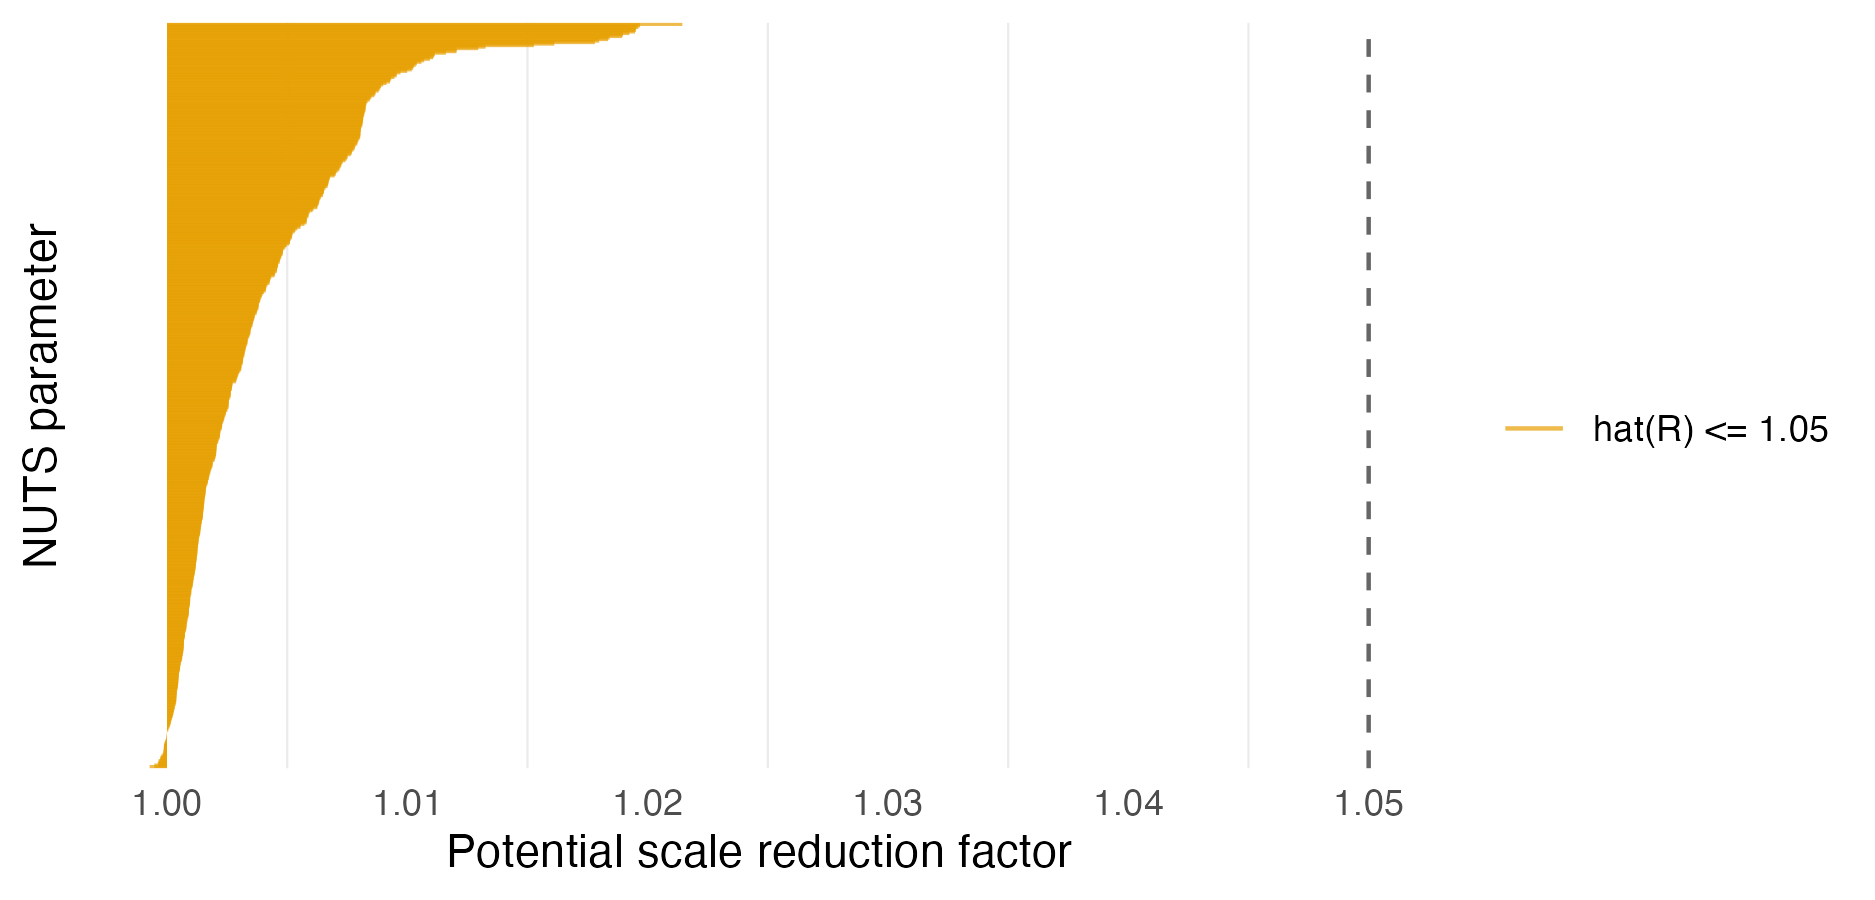
\includegraphics[width=0.95\linewidth]{resources/naomi-aghq/20230811-095752-5b8181d8/depends/rhat} 

}

\caption{The potential scale reduction factor compares between- and within- estimates of univariate parameters. It is recommended only to use NUTS results if the value is less than 1.05, which it is for all parameters.}\label{fig:rhat}
\end{figure}


%%%%% REFERENCES

% JEM: Quote for the top of references (just like a chapter quote if you're using them).  Comment to skip.
% \begin{savequote}[8cm]
% The first kind of intellectual and artistic personality belongs to the hedgehogs, the second to the foxes \dots
%   \qauthor{--- Sir Isaiah Berlin \cite{berlin_hedgehog_2013}}
% \end{savequote}

\setlength{\baselineskip}{0pt} % JEM: Single-space References

{\renewcommand*\MakeUppercase[1]{#1}%
\printbibliography[heading=bibintoc,title={\bibtitle}]}


\end{document}
